\documentclass[11pt]{scrartcl}
\usepackage{booktabs}
\usepackage{bbding}

\usepackage[utf8]{inputenc}
\usepackage{adjustbox}
\usepackage[main=vietnamese,english]{babel}
\usepackage{enumitem}
\usepackage{booktabs}
\usepackage{bbding}
\usepackage{graphicx}
\usepackage{titletoc}
\usepackage{eso-pic}
\usepackage{tikz}
\usepackage{tcolorbox}
\usepackage{fancyhdr}
\usepackage{listings}
\usepackage{subfig}
\usepackage{wrapfig}

\usepackage[a4paper, left=1in, right=1in, top=0.7in, bottom=1in]{geometry}
\usepackage{setspace}
\usepackage[normalem]{ulem}
\usepackage{amsthm}
\definecolor{dk}{rgb}{0,0,0}
\newcommand{\vocab}[1]{\textbf{\color{black}\sffamily #1}}
\newcommand{\vocabsh}[1]{\textbf{\color{c}\sffamily #1}}
\newcommand{\vocabh}[1]{\textbf{\color{mauve}\sffamily #1}}
\newcommand{\vocabf}[1]{\textit{\sffamily #1}}
\onehalfspacing % Chọn 1.5 khoảng cách giữa các dòng
\usepackage{enumitem}
\usepackage{amssymb} % for \blackcircle
\usepackage{amsmath}
\usepackage[framemethod=TikZ]{mdframed}
\definecolor{bk}{rgb}{0.0, 0.0, 0.61}
\definecolor{p}{rgb}{0.1, 0.1, 0.44}
\definecolor{c}{rgb}{0.55, 0.27, 0.07}
\newtheorem{lemma}{Bổ đề}
\newtheorem{theorem}{\textcolor{p}{Định lý}}
\usepackage{pifont}
\usepackage{mathtools}
\usepackage{etextools}
\usepackage{ifthen}
\usepackage{hyperref}
\usepackage{lmodern}
\renewcommand*\contentsname{\LARGE MỤC LỤC}
\renewcommand\familydefault{\sfdefault}
\renewcommand{\proofname}{\vocab{Lời giải}}

\renewcommand{\thesection}{\LARGE\textcolor{dk}{\arabic{section}}}
\renewcommand{\thesubsection}{\large \Alph{subsection} }
\newtheorem{m}{\textcolor{p}{Mệnh đề}}
\newtheorem{baitoan}{\vocab{\textit{Bài toán}}}[section]
\newtheorem{bod}{\vocab{Bổ đề}}[section]
\usepackage{chngcntr}
\newtheorem{g}{\begin{center}\textbf{\textcolor{p}{Bài giải}}\end{center}}
\usepackage[inline]{asymptote}
\newtheorem{btv}{\vocab{Bài toán}}[section]
\definecolor{y}{rgb}{1.0, 0.88, 0.21}
\usepackage{CJKutf8}
\pagestyle{fancy}
\usepackage{multido}

\newcommand{\Pointilles}[1]{%
  \par\nobreak
  \noindent\rule{0pt}{1.5\baselineskip}% Provides a larger gap between the preceding paragraph and the dots
  \multido{}{#1}{\noindent\makebox[\linewidth]{\dotfill}\endgraf}% ... dotted lines ...
  \bigskip% Gap between dots and next paragraph
}
% Redefine \Leftrightarrow to \Lra
\let\lra\Leftrightarrow
\let\Leftrightarrow\relax
\newcommand{\ov}{\overline}
\newcommand{\fra}{\forall}
\newcommand{\xyr}{\forall x,y \in \bb{R}}
\newcommand{\xr}{\forall x\in \bb{R}}
\newcommand{\yr}{\forall y\in \bb{R}}
\newcommand{\xyro}{\forall x,y \in \bb{R^+}}
\newcommand{\xro}{\forall x\in \bb{R^+}}
\newcommand{\yro}{\forall y\in \bb{R^+}}
\newcommand{\bb}{\mathbb}
\newcommand{\dbi}{\displaystyle\binom}
\newcommand{\dsum}{\displaystyle\sum}
\newcommand{\dlim}{\displaystyle\lim_{n \to +\infty}}
\newcommand{\blim}{\displaystyle\lim}
\newcommand{\dprod}{\displaystyle\prod}
\newcommand{\dint}{\displaystyle\int}
\newcommand{\csum}{\dsum_{cyc}}
% Redefine \Rightarrow to \Ra
\let\ra\Rightarrow
\let\Rightarrow\relax
\definecolor{dkgreen}{rgb}{0,0.6,0}
\definecolor{gray}{rgb}{0.5,0.5,0.5}
\definecolor{mauve}{rgb}{0.58,0,0.82}
\newcommand{\DeclarePairedDelimiterCase}[2]{%
\newcommand#1[1][]{%
	\ifthenelse{\equal{##1}{normal}}%
	{#2}%
	{%
		\ifthenelse{\equal{##1}{big}\OR\equal{##1}{Big}\OR\equal{##1}{bigg}\OR\equal{##1}{Bigg}}%
		{\expandnext{#2[}{\csname##1\endcsname}]}%
		{#2*}%        % standard case using \left and \right
	}%
}%
}
\newcommand{\DeclarePairedDelimiterY}[4][Temp]{%
\expandafter\DeclarePairedDelimiter\csname#2#1\endcsname{#3}{#4}%
\expandnext{\expandnext{\DeclarePairedDelimiterCase}{\csname#2\endcsname}}{\csname#2#1\endcsname}%
}
\newcommand{\DeclarePairedDelimiterXY}[6][Temp]{%
\expandafter\DeclarePairedDelimiterX\csname#2#1\endcsname[#3]{#4}{#5}{#6}%
\expandnext{\expandnext{\DeclarePairedDelimiterCase}{\csname#2\endcsname}}{\csname#2#1\endcsname}%
} 
\DeclarePairedDelimiter\floor{\lfloor}{\rfloor}

\lstset{
  frame=none, % Xóa khung ở trên và dưới
  language=Python,
  aboveskip=3mm,
  belowskip=3mm,
  showstringspaces=false,
  columns=flexible,
  basicstyle={\small\ttfamily},
  numbers=none,
  keywordstyle=\color{blue},      % Màu sắc cho các từ khóa
  commentstyle=\color{green!60},  % Màu sắc cho các comment
  stringstyle=\color{brown},        % Màu sắc cho chuỗi
  numberstyle=\tiny\color{gray},  % Màu sắc cho số dòng
  breaklines=true,
  breakatwhitespace=true,
  tabsize=3
}
\renewcommand{\headrulewidth}{0.005em}

\makeatother
\makeatletter

\fancypagestyle{plain}{%
	\fancyhf{}%
	\fancyfoot[C]{\thepage}
	\renewcommand{\headrulewidth}{0pt}%
}

\newcommand{\circled}[1]{\tikz[baseline=(char.base)]{
		\node[shape=circle,fill,inner sep=3pt,text=white] (char) {\footnotesize #1};}}
\renewcommand{\arraystretch}{1.5}
\let\oldfrac\frac
\renewcommand{\frac}[2]{\displaystyle\oldfrac{#1}{#2}}
% Định nghĩa môi trường mới
\newmdenv[linecolor=black, linewidth=0.02cm]{myframe}
\newmdenv[linecolor=bk, backgroundcolor=blue!4,  linewidth=0.04	cm]{fr}
% Môi trường "bài toán"
\newenvironment{bt}
{
	\color{p}\begin{myframe}
		\begin{baitoan}%\upshape
		}
		{
		\end{baitoan}
	\end{myframe}
}
\newenvironment{bd}
{
	
		
		\begin{bod}\upshape
		}
		{
		\end{bod}

}
\newenvironment{thr}
{
	\color{p}\begin{fr}
		\begin{theorem}\upshape
		}
		{
		\end{theorem}
	\end{fr}
}
\newenvironment{md}
{\m\upshape}
{\endm}
\newenvironment{btvn}
{
	
		
		\begin{btv}%\upshape
		}
		{
		\end{btv}

}
\renewcommand\proofname{}
\newenvironment{sol}{%
        \begin{proof}[\unskip\nopunct]%
	\vocab{Lời giải.}
}{% 
        \end{proof}%
}
\newenvironment{pro}{%

	\textbf{\vocab{Chứng minh}}%

\begin{proof}[\unskip\nopunct]%
}{\end{proof}%
}

\renewcommand\them{\textcolor{p}{\arabic{m}}}
\renewcommand\thebtv{\vocab{\arabic{btv}}}

\newcommand{\p}[1]{\textbf{\textcolor{p}{#1}}}
\newcommand{\pf}[1]{\textit{\textcolor{p}{#1}}}
\renewcommand\thebaitoan{\vocab{\arabic{baitoan}}}
\renewcommand\thebod{\vocab{\arabic{bod}}}
\newcounter{theo}[section]\setcounter{theo}{0}
\renewcommand{\thetheo}{\arabic{section}.\arabic{theo}}
\newenvironment{theo}[2][]{%
	\refstepcounter{theo}%
	\ifstrempty{#1}%
	{\mdfsetup{%
			frametitle={%
				\tikz[baseline=(current bounding box.east),outer sep=0pt]
				\node[anchor=east,rectangle,fill=yellow]
				{\strut };}}
	}%
	{\mdfsetup{%
			frametitle={%
				\tikz[baseline=(current bounding box.east),outer sep=0pt]
				\node[anchor=east,rectangle,fill=yellow!70, draw=black, line width=0.03cm]
				{\strut \vocab{#1}};}}%
	}%
	\mdfsetup{innertopmargin=5pt,linecolor=black,%
		linewidth=0.03cm,topline=true,%
		frametitleaboveskip=\dimexpr-\ht\strutbox\relax, 
	}
	\begin{mdframed}[]\relax%
		\label{#2}}{\end{mdframed}}
	
\newcounter{lem}[section]\setcounter{lem}{0}
\renewcommand{\thelem}{\arabic{section}.\arabic{lem}}
\newenvironment{lem}[2][]{%
	\refstepcounter{lem}%
	\ifstrempty{#1}%
	{\mdfsetup{%
			frametitle={%
				\tikz[baseline=(current bounding box.east),outer sep=0pt]
				\node[anchor=east,rectangle,fill=yellow]
				{\strut };}}
	}%
	{\mdfsetup{%
			frametitle={%
				\tikz[baseline=(current bounding box.east),outer sep=0pt]
				\node[anchor=east,rectangle,fill=yellow]
				{\strut \vocab{#1}};}}%
	}%
	\mdfsetup{linecolor=black,%
		linewidth=0.03cm,topline=true,%
		frametitleaboveskip=\dimexpr-\ht\strutbox\relax
	}
	\begin{mdframed}[]\relax%
		\label{#2}}{\end{mdframed}}
		\newcommand{\fa}{%
		\begin{tikzpicture}[x=1.4ex, y=1.4ex, scale=0.5, baseline=-.8ex]
			\draw (-1,1)  -- (-1,0) -- (1,0) -- (1,-1);
			\draw (-1,-1) -- (0,-1) -- (0,1) -- (1,1);
		\end{tikzpicture}%
	}
	
	\newcommand{\func}[1]{f\left(#1\right)}
	\renewcommand*\l@section[2]{%
	
	\ifnum\c@tocdepth>\@ne
	  
	  \addpenalty\@secpenalty
	  \addvspace{1.3em \@plus\p@}% increase space between line and section
	  \setlength\@tempdima{2em}%
	  \begingroup
	  	\large
		\parindent \z@ \rightskip \@pnumwidth
		\parfillskip -\@pnumwidth
		\bfseries #1\leavevmode
		\hfil \hbox to \@pnumwidth{\hss #2}\par
		\kern 5pt
		\hrule
		\kern 1pt
	  \endgroup
	\else
	  \addvspace{1.0em \@plus\p@}%
	\fi}
	\renewcommand\l@subsection[2]{%
	\ifnum\c@tocdepth>\@ne
	  \addpenalty\@secpenalty
	  \addvspace{1em \@plus\p@}% increase space between line and section
	  \setlength\@tempdima{2em}%
	  \begingroup
		\large
		\parindent \z@ \rightskip \@pnumwidth
		\parfillskip -\@pnumwidth
		\advance\leftskip\@tempdima
		\normalfont #1\leavevmode
		\hfil \hbox to \@pnumwidth{\hss #2}\par
		\kern 5pt
		\hrule
		\kern 1pt
	  \endgroup
	\else
	  \addvspace{1.0em \@plus\p@}%
	\fi}
  \makeatother

\RedeclareSectionCommand[
  tocnumwidth=3em % Điều chỉnh độ rộng của số trang trong mục lục
]{section}
\RedeclareSectionCommand[
  tocindent=3em, % Điều chỉnh khoảng cách lề trái của mục
  tocnumwidth=3.5em % Điều chỉnh độ rộng của số trang trong mục lục
]{subsection}

\lhead{\today}
\rhead{\begin{CJK}{UTF8}{ipxm} カズマアカリ。
\end{CJK}}
\usepackage{pdfpages}
\begin{document}

\title{\vspace{-2em}\textcolor{bk}{\textbf{BÀI TẬP TỔ HỢP VÀ ĐẠI SỐ}}}

%\subtitle{\vspace{1.5em}{\textbf{\LARGE CAUCHY-SCHWARZ-HOLDER}}}
\author{Phạm Bảo -\begin{CJK}{UTF8}{ipxm} カズマアカリ。\end{CJK}\vspace{-1em}}

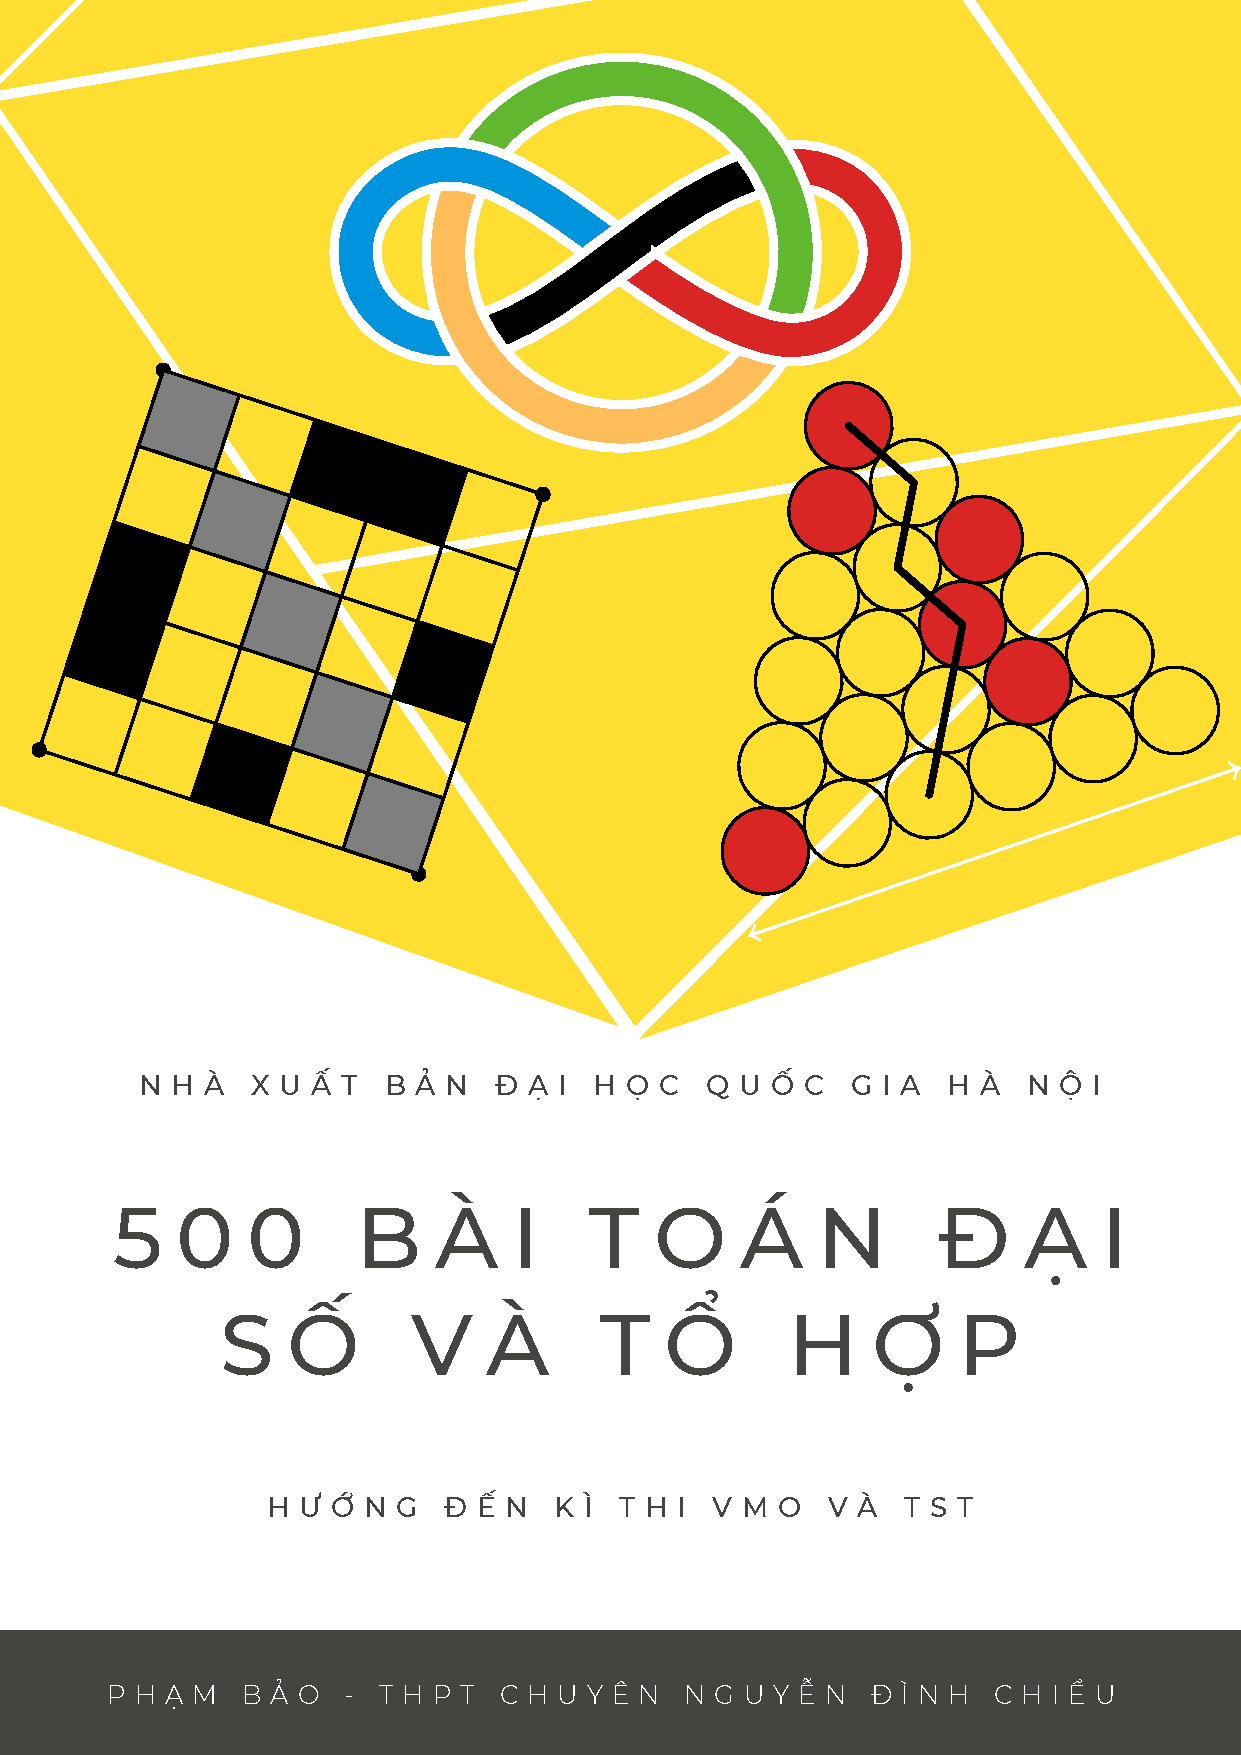
\includepdf[pages=1]{bia.pdf}
%\maketitle
\thispagestyle{empty}

\tableofcontents

%\subsection*{\Large\textcolor{bk}{ \S 1.1.} Các bất đẳng thức cổ điển}
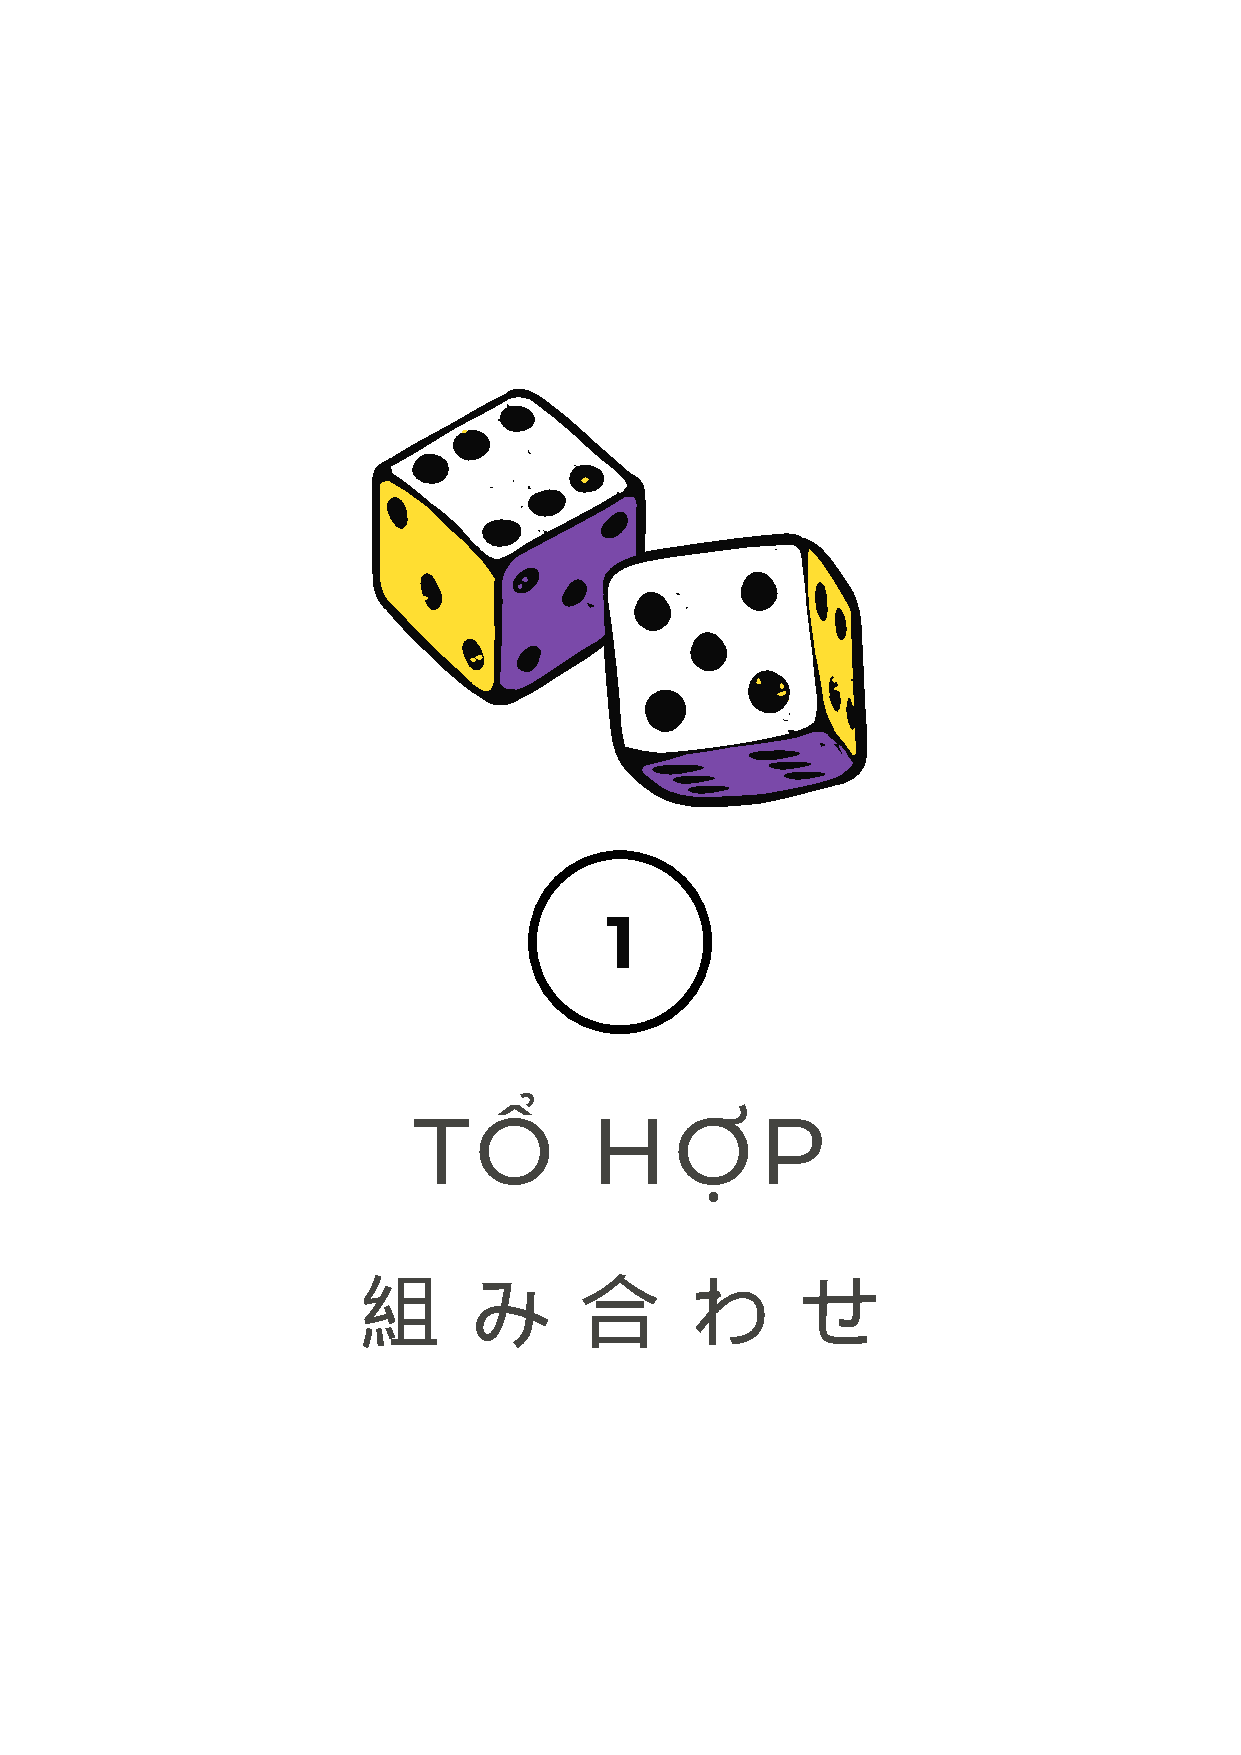
\includepdf[pages=1]{1.pdf}
\section{\huge Tổ hợp}
\subsection{\LARGE \textcolor{dk}{Đề bài}}

\setcounter{page}{1}
\thispagestyle{plain}
\begin{itemize}[label=, leftmargin=0em, itemsep=-0em]
    
    \item \begin{btvn}%\vocab{(AIME 1996).} 
        Một học sinh chán nản đi dọc hành lang có các tủ khóa, được đánh số từ 1 đến 1024. Anh ta mở cửa số 1, sau đó luân phiên hành động bỏ qua hoặc mở các tủ khóa kế đó. Khi anh ta đi đến cuối hành lang, anh ta quay đầu và tiếp tục. Anh ta mở chiếc tủ đầu tiên bị khóa, sau đó tương tự lặp lại ngẫu nhiên những thao tác. Anh ta cứ liên tục làm vậy cho đến khi tất cả các tủ đều mở. Hỏi tủ cuối cùng còn khóa là số mấy?
    \end{btvn}

    \item \begin{btvn}\vocab{(IMOSL 1996).} Cho một bảng ô vuông $(n - 1)\times(n - 1)$. Trong $n^2$ cạnh của bảng đó được tô bởi màu xanh hoặc đỏ. Tìm số cách tô màu khác nhau sao cho mỗi hình vuông đơn vị có ít nhất hai cạnh đỏ
    \end{btvn}

    \item\begin{btvn}%\vocab{(AIME 1985).} 
        Trong một giải đấu mỗi người chơi đúng một trận với người khác. Trong mỗi trận đấu người chiến thắng giành được 1 điểm, thua được 0 điểm, hòa nhau thì mỗi bên được 0.5 điểm. Sau giải đấu, có chính xác một nửa số điểm thuộc về mỗi người chơi nhận được trong những trận đấu với 10 người đứng chót bảng xếp hạng. Hỏi số tổng điểm của các người chơi trong giải đấu là bao nhiêu?
    \end{btvn}

    \item \begin{btvn}%\vocab{(USAMO 1999).} 
        Cho số nguyên dương $n > 1$ lẻ. Tìm số hoán vị $p$ của tập hợp $[n]$ thỏa mãn
    \[
        |p(1) - 1| + |p(2) - 2| +\dots + |p(n) -n| = \frac{n^2 - 1}{2}
    \]
        
    \end{btvn}

    \item \begin{btvn}\vocab{(HMMT 02/2016).} Cho số nguyên lẻ $n > 1$. Trên một bàn cờ $n \times n$ có ô trung tâm và 4 ô ở góc bị cắt đi. Chúng ta muốn chia $n^2 -5$ hình vuông còn lại thành $\frac{1}{2}(n^2 - 5)$ cặp sao cho hai hình vuông ở mỗi cặp giao nhau tại chính xác một điểm. Tìm giá trị của $n$ thỏa mãn điều đó.
    \end{btvn}

    \item \begin{btvn}\vocab{(USAJMO 2019).}
        Có $a+b$ cái bát được sắp xếp thành một hàng ngang, được đánh số từ $1$ đến $a+b$. Ban đầu, $a$ bát đầu tiên chứa một quả táo và $b$ bát cuối cùng chứa một quả lê.
        Một nước đi được gọi là hợp lệ bao gồm việc chuyển một quả táo từ bát $i$ sang bát $i+1$ và một quả lê từ bát $j$ sang bát $j-1$, với điều kiện là sự chênh lệch $i-j$ là chẵn. nhiều loại trái cây có thể nằm trong cùng một bát cùng một lúc. Mục tiêu là có được $b$ bát đầu tiên, mỗi bát chứa một quả lê và $a$ bát cuối cùng, mỗi bát chứa một quả táo. Chứng minh rằng điều này có thể xảy ra khi và chỉ nếu tích $ab$ là số chẵn.
    \end{btvn}

    \item \begin{btvn}\vocab{\href{https://artofproblemsolving.com/community/c6h2687948p23322888}{(Pan-African Girls MO 2021).}}
    Lucía nhân một vài số dương có một chữ số (không nhất thiết phải phân biệt) và thu được một số $n$ lớn hơn 10. Sau đó, cô nhân tất cả các chữ số của $n$ và thu được một số lẻ. Tìm tất cả các giá trị có thể có của chữ số hàng đơn vị của $n$.        
    \end{btvn}

    \item \begin{btvn}\vocab{(USAJMO 2016).}
        Tìm số nguyên nhỏ nhất $N$ sao cho nếu loại bỏ bất kỳ $2016$ phần tử nào khỏi tập hợp ${1, 2,...,N}$, vẫn có thể tìm được $2016$ số phân biệt trong số các phần tử còn lại có tổng bằng $N$.
    \end{btvn}

    \item \begin{btvn}\vocab{(IMO 1974).}
    Cho một dãy tăng tuyến tính $a_1 < a_2 <\dots< a_p$ và xét phân hoạch của một bàn cờ $8\times 8$ thành $p$ hình chữ nhật không giao nhau, thoả mãn các điều kiện sau:

    \begin{enumerate}
        \item Mỗi hình chữ nhật có số ô trắng bằng số ô đen.
        \item Nếu $a_i$ là số ô trắng trong hình chữ nhật thứ $i$, thì $a_1<a_2<\ldots <a_p$.
        Tìm giá trị lớn nhất của $p$ sao cho phân rã như vậy là có thể. Đối với giá trị của $p$ này, xác định tất cả các dãy số có thể $a_1,a_2,\ldots ,a_p$.
    \end{enumerate}
    \end{btvn}

    \item \begin{btvn}\vocab{(USAMO 2012).}
    Tìm tất cả các số nguyên $n \geq 3$ sao cho với mọi $n$ số thực dương $a_1, a_2, \hdots, a_n$ với 
    \[\text{max}(a_1,a_2,\hdots,a_n) \leq n \cdot \text{min}(a_1,a_2,\hdots,a_n)\]
    luôn tồn tại ba số là độ dài các cạnh của một tam giác nhọn.
    \end{btvn}
    
    \item \begin{btvn}\vocab{\href{https://www.facebook.com/ToanHocvoiPsi/posts/1319983838702201}{(KHTN Lớp 10 - 2023).}}
        Viết một trăm số nguyên dương đầu tiên $1,2,\dots,100$ vào một bảng ô vuông kích thước $10\times 10$ một cách tùy ý sao cho mỗi ô được viết đúng một số. Chứng minh rằng tồn tại hai ô kề nhau (2 ô có cạnh chung) mà hai số viêt ở hai ô này có hiệu lớn hơn hoặc bằng 10.
    \end{btvn}
    \item \begin{btvn}\vocab{(IMO 2017).}
        Đối với mỗi số nguyên $a_0 > 1$, xác định dãy $a_0, a_1, a_2, \ldots$ với $n \geq 0$ như sau:
        $$
        \begin{cases}
        \sqrt{a_n} & \text{nếu } \sqrt{a_n} \text{ là một số nguyên,} \\
        a_n + 3 & \text{ngược lại.}
        \end{cases}
        $$
    Xác định tất cả các giá trị của $a_0$ sao cho tồn tại một số $A$ sao cho $a_n = A$ cho vô số giá trị của $n$.
    \end{btvn}

    \item \begin{btvn}\vocab{\href{https://artofproblemsolving.com/community/c6h2687946p23323816}{(Pan-African Girls MO 2021).}}
    Có $n \geq 2$ đồng xu được đánh số từ $1$ đến $n$. Các đồng xu này được đặt xung quanh một vòng tròn, không nhất thiết theo thứ tự.
    
    Trong mỗi lượt, nếu chúng ta đang ở đồng xu có số $i$, chúng ta sẽ nhảy đến đồng xu ở vị trí $i$ đơn vị từ nó, luôn theo hướng kim đồng hồ, bắt đầu từ đồng xu số 1. Ví dụ, xem hình dưới đây.
    
    Tìm tất cả các giá trị của $n$ để tồn tại một sắp xếp của các đồng xu trong đó mỗi đồng xu sẽ được ghé thăm.
    \end{btvn}

    \item \begin{btvn}\vocab{\href{https://artofproblemsolving.com/community/c6h2687954p23322931}{(Pan-African Girls MO 2021).}}
        Celeste có một lượng không giới hạn của mỗi loại trong $n$ loại kẹo, được đánh số từ loại 1, loại 2, ... loại $n$. Ban đầu, cô ấy lấy $m>0$ miếng kẹo và đặt chúng thành một hàng trên bàn. Sau đó, cô ấy chọn một trong các phép toán sau (nếu có sẵn) và thực hiện nó:
        \begin{enumerate}
            \item Cô ăn một viên kẹo của loại $k$, và tại vị trí đó trong hàng cô đặt một viên kẹo loại $k-1$ tiếp theo là một viên kẹo loại $k+1$ (chúng ta coi loại $n+1$ là loại 1, và loại 0 là loại $n$).
            \item Cô chọn hai viên kẹo liên tiếp có cùng loại, và ăn chúng.
        \end{enumerate}
        Tìm tất cả các số nguyên dương $n$ để Celeste có thể rời bàn trống cho bất kỳ giá trị của $m$ và bất kỳ cấu hình kẹo trên bàn nào.
    \end{btvn}

    \item \begin{btvn}\vocab{(IMC 2002).}
        Một kì thi Olympic có sáu bài toán và 200 thí sinh. Các thí sinh rất giỏi, vì vậy mỗi bài toán được giải bởi ít nhất 120 thí sinh. Chứng minh rằng luôn tồn tại ít nhất hai thí sinh sao cho mỗi bài toán được giải bởi ít nhất một trong họ.
    \end{btvn}

    \item \begin{btvn}\vocab{(Canada MO 2006).}
        Trong một giải đấu vòng tròn với $2n+1$ đội, trong đó mỗi đội chơi với mỗi đội khác đúng một trận. Chúng ta nói rằng ba đội $X,Y$ và $Z$ tạo thành một bộ ba chu trình nếu $X$ đánh bại $Y$, $Y$ đánh bại $Z$ và $Z$ đánh bại $X$ và không có trận hòa.
        \begin{enumerate}[label=(\alph*)]
            \item Xác định số lượng tối thiểu của các bộ ba chu trình có thể.
            \item  Xác định số lượng tối đa của các bộ ba chu trình có thể.
        \end{enumerate}        
    \end{btvn}
    \item \begin{btvn}\vocab{(IMO 1993).} Trên bàn cờ vô hạn ta thực hiện một trò chơi như sau: Đầu tiên xếp $n^2$ quân vào một hình vuông gồm $n \times n$ ô vuông cạnh liền kề sao cho trong mỗi ô vuông của hình vuông chứa một quân cờ, cách đi trong trò chơi là quân cờ chỉ được nhảy theo một chiều ngang hoặc chiều dọc qua một ô có chứa quân cờ ở ngay sát bên cạnh sang một bên ô trống tiếp ngay sau đó. Khi đó quân cờ ô bị nhảy qua sẽ bị loại bỏ. Tìm các giá trị của $n$ để có thể kết thúc trò chơi sao cho trên bàn cờ chỉ còn lại đúng một quân cờ.
    \end{btvn}


    \item\begin{btvn}\vocab{(AIME 1985).}
        Trong một giải đấu, mỗi người chơi chơi chính xác một trận đấu với mỗi người chơi khác. Trong mỗi trận đấu, người thắng được thưởng 1 điểm, người thua nhận 0 điểm, và mỗi trong hai người chơi nhận được 1/2 điểm nếu trận đấu hòa. Sau khi hoàn thành giải đấu, được phát hiện rằng chính xác một nửa số điểm mà mỗi người chơi kiếm được đã được kiếm trong các trận đấu chống lại mười người chơi có số điểm thấp nhất. (Cụ thể, mỗi trong số mười người chơi có số điểm thấp nhất đã kiếm được một nửa số điểm của mình trong các trận đấu chống lại các người chơi còn lại trong số mười người đó). Tổng số người chơi trong giải đấu là bao nhiêu?
    \end{btvn}

    \item \begin{btvn}\vocab{(ELMO 2015).}
        Cho các số nguyên dương $m$, $n$, và $x$. Chứng minh rằng
        \[ \sum_{i = 1}^n \min\left(\left\lfloor \frac{x}{i} \right\rfloor, m \right) = \sum_{i = 1}^m \min\left(\left\lfloor \frac{x}{i} \right\rfloor, n \right). \]
        
    \end{btvn}
    \item \begin{btvn}\vocab{(Russia 1996).}
        Ở thành phố Duma có 1600 đại biểu, họ đã thành lập 16000 ủy ban mỗi ủy ban có 80 người. Chứng minh rằng có thể tìm thấy hai ủy ban có ít nhất bốn thành viên chung.
    \end{btvn}
    \item \begin{btvn}\vocab{(IMOSL 1998).}
        Trong một cuộc thi, có $m$ ứng viên và $n$ giám khảo, với $n\geq 3$ là một số lẻ. Mỗi ứng viên được đánh giá bởi mỗi giám khảo là đạt hoặc không đạt. Giả sử mỗi cặp giám khảo đồng ý với tối đa $k$ ứng viên. Chứng minh rằng
        \[{\frac{k}{m}} \geq {\frac{n-1}{2n}}. \]
    \end{btvn}
    \begin{btvn}\vocab{(Bay Area MO 2013).}
        Cho số nguyên dương $n>2$, xét $n-1$ phân số
        \[
            \frac{2}{1},\frac{3}{2},\dots,\frac{n}{n - 1}
        \]
        Tích của các phân số này bằng $n$, nhưng nếu bạn lấy nghịch đảo (tức là đảo ngược) một số trong các phân số, tích sẽ thay đổi. Bạn có thể làm cho tích bằng 1 không? Tìm tất cả các giá trị của $n$ mà điều này là có thể và chứng minh rằng bạn đã tìm được tất cả chúng.
    \end{btvn}

    \item \begin{btvn}\vocab{(USAMO 2012).}
        Một đường tròn được chia thành $432$ cung đồng nhất bởi $432$ điểm. Các điểm được tô màu bằng bốn màu sao cho một số $108$ điểm được tô màu Đỏ, một số $108$ điểm được tô màu Xanh lá cây, một số $108$ điểm được tô màu Xanh dương, và $108$ điểm còn lại được tô màu Vàng. Chứng minh rằng có thể chọn ba điểm của mỗi màu sao cho bốn tam giác được tạo thành bởi các điểm được chọn cùng màu đó là đồng dạng.
    \end{btvn}

    

    \item \begin{btvn}\vocab{(Online Math Open 2013.)}
        Kevin có $255$ chiếc bánh quy, mỗi chiếc đều được gắn nhãn bằng một tập con duy nhất không rỗng của ${1,2,3,4,5,6,7,8}$. Mỗi ngày, anh ta chọn ngẫu nhiên một chiếc bánh quy từ những chiếc bánh quy chưa ăn. Sau đó, anh ấy ăn chiếc bánh đó, và tất cả các chiếc bánh còn lại có nhãn là một tập con của chiếc bánh đó (ví dụ, nếu anh ấy chọn chiếc bánh được gắn nhãn là ${1,2}$, anh ấy sẽ ăn chiếc bánh đó cũng như các chiếc bánh với nhãn là ${1}$ và ${2}$). Giá trị kỳ vọng của số ngày mà Kevin ăn một chiếc bánh trước khi hết tất cả các chiếc bánh có thể được biểu diễn dưới dạng $\frac{m}{n}$, trong đó $m$ và $n$ là các số nguyên dương tương đối nguyên tố. Tìm $m + n$.
    \end{btvn}

    \item \begin{btvn}\vocab{(USAMO 2017).}
        Cho $P_1$, $P_2$, $\dots$, $P_{2n}$ là $2n$ điểm phân biệt trên đường tròn đơn vị $x^2+y^2=1$, trừ điểm $(1,0)$. Mỗi điểm được tô màu đỏ hoặc xanh, với đúng $n$ điểm đỏ và $n$ điểm xanh. Hãy cho $R_1$, $R_2$, $\dots$, $R_n$ là một thứ tự bất kỳ của các điểm đỏ. Hãy cho $B_1$ là điểm xanh gần nhất với $R_1$ theo hướng kim đồng hồ điều chỉnh quanh đường tròn bắt đầu từ $R_1$. Sau đó hãy cho $B_2$ là điểm xanh gần nhất với $R_2$ trong các điểm xanh còn lại điều chỉnh theo hướng kim đồng hồ từ $R_2$, và tiếp tục như vậy, cho đến khi chúng ta đánh dấu tất cả các điểm xanh là $B_1, \dots, B_n$. Chứng minh rằng số lượng cung điều chỉnh theo hướng kim đồng hồ có dạng $R_i \to B_i$ chứa điểm $(1,0)$ không phụ thuộc vào cách chúng ta chọn thứ tự $R_1, \dots, R_n$ của các điểm đỏ.
    \end{btvn}

    \item \begin{btvn}
        Giả sử có 4951 điểm phân biệt trên mặt phẳng sao cho không có bốn điểm nào thẳng hàng. Chứng minh rằng có thể chọn 100 trong số các điểm đó mà không có ba điểm nào thẳng hàng.
    \end{btvn}

    \item \begin{btvn}\vocab{(Putnam 1979).}
        Cho $n$ điểm màu đỏ và $n$ điểm màu xanh dương trong mặt phẳng, không có ba điểm nào thẳng hàng. Chứng minh rằng chúng ta có thể vẽ $n$ đoạn thẳng, mỗi đoạn nối một điểm đỏ với một điểm xanh dương, sao cho không có đoạn nào cắt nhau.
    \end{btvn}

    \item \begin{btvn}\vocab{(Princeton Competition 2013).}
        Cho đồ thị $G$ gồm một tập hợp các đỉnh, một số trong số đó được kết nối bởi các cạnh (vô hướng). Một tập hợp các cạnh có một điểm cuối chung được gọi là \textit{ngôi sao}. Một ghép cặp của đồ thị là một tập hợp các cạnh sao cho không có hai cạnh nào có một điểm cuối chung. Chứng minh rằng nếu số lượng cạnh của đồ thị $G$ lớn hơn $2(k-1)^2$, thì $G$ chứa một ghép cặp có kích thước $k$ hoặc một ngôi sao có kích thước $k$.
    \end{btvn}

    \item \begin{btvn}\vocab{(IMOSL 2013).}
        Cho $n$ là một số nguyên dương. Tìm số nguyên nhỏ nhất $k$ với tính chất sau: Cho bất kỳ các số thực $a_1 , \cdots , a_d $ sao cho $a_1 + a_2 + \cdots + a_d = n$ và $0 \le a_i \le 1$ với $i=1,2,\cdots ,d$, ta có thể phân chia các số này thành $k$ nhóm (một số trong số đó có thể là rỗng) sao cho tổng của các số trong mỗi nhóm không vượt quá $1$.
    \end{btvn}

    \item \begin{btvn}\vocab{(IMOSL 2003)}
        Cho $A$ là một tập con gồm $101$ phần tử của tập $S=[1000000]$. Chứng minh rằng tồn tại các số $t_1$, $t_2, \ldots, t_{100}$ trong $S$ sao cho các tập\[ A_j=\{x+t_j\mid x\in A\},\qquad j=1,2,\ldots,100  \]là đôi một không giao nhau.
    \end{btvn}
    \item \begin{btvn}\vocab{(PTNK 2019 Lớp 10).}
        Cho tập hợp $X = \{1,2,\dots,396\}$. Gọi $S_1,S_2,\dots,S_k$ là $k$ tập con khác nhau của $X$ thỏa mãn đồng thời hai điều kiện sau:
        \begin{enumerate}
            \item $|S_1| = |S_2| = \dots = |S_k| = 198$.
            \item $|S_i \cap S_j| \leq 99, \forall i,j \in \mathbb{N}^*, 1 \leq i \leq j \leq k$
        \end{enumerate}
        Chứng minh rằng $k \leq 6^{50}$.
    \end{btvn}
    \item \begin{btvn}\vocab{(PTNK 2019).}
        Cho $n$ số thực $x_1, x_2,\dots,x_n$. Với mỗi $i \in \{1,2,\dots,n\}$, gọi $a_i$ là các chỉ số $j$ mà $|x_i  - x_j| \leq 1$ và $b_i$ là các chỉ số $j$ mà $|x_i - x_j| \leq 2$ ($i$ và $j$ có thể bằng nhau).
        \begin{enumerate}
            \item Chứng minh rằng tồn tại $i$ để $b_i \leq 3a_i$.
            \item Gọi $A$ là số cặp $(i,j)$ có thứ tự mà $|x_i - x_j| \leq 1$ và $B$ là số cặp $(i,j)$ có thứ tự mà $|x_i - x_j| \leq 2$. Chứng minh rằng $B \leq 3A$.
        \end{enumerate}
    \end{btvn}
    \item\begin{btvn}\vocab{(Japan MO Final 2016 P3). }
        Cho $n$ là một số nguyên dương. Trong vương quốc Skibidi có $2^n$ công dân và một vị vua. Trong ngôn ngữ tiền tệ, vương quốc sử dụng các tờ giấy bạc có mệnh giá là $2^n$ đồng và các đồng xu có mệnh giá là $2^a$ (với $a=0,1,\ldots,n-1$). Mỗi công dân có vô số tờ giấy bạc. Gọi $S$ là tổng số đồng xu trong vương quốc. Một ngày đẹp trời, vua quyết định triển khai một chính sách sẽ được thực hiện mỗi đêm:
        \begin{enumerate}
            \item Mỗi công dân phải quyết định một số tiền hữu hạn dựa trên số đồng xu mà anh ta hiện đang có, và anh ta phải chuyển số tiền đó cho một công dân khác hoặc cho vua.
            \item Mỗi công dân phải chuyển chính xác nhiều hơn $\$1$ số tiền mà anh ta nhận được từ một công dân khác. 
            \item Luôn phải có một công dân kết thúc quá trình này bằng cách đưa tiền cho vua.
        \end{enumerate}

        Tìm giá trị nhỏ nhất của $S$ sao cho vua có thể thu tiền mỗi đêm mà không bao giờ hết tiền.
    \end{btvn}

    \begin{comment}
        Tuy mỗi người có vô hạn tiền giấy, nhưng lại có hữu hạn xu. Vậy nên người cuối cùng đưa tiền cho vua phải đưa $k$ tờ tiền $2^n$ và ta gọi cách chuyển tiền này là $\mathbb{H}$. Ta hãy xét thuật toán như sau:

        Để chuyển tiền thỏa mãn $\mathbb{H}$, người đầu tiên phải đưa một số tiền bằng $k2^n$ với $k \geq 1$, vì ta muốn $S$ nhỏ nhất nên ta có thể tối ưu bằng cách để anh ta đưa $k$ tờ tiền giấy. Và mỗi người tiếp theo là $2,3,\dots,2^{n} - 1$ sẽ góp $\$1$ xu vào đến người thứ $2^n$ số tiền góp lại hiện tại là $(k + 1)2^n$ tính cả người thứ $2^n$ đã góp vào, vì tiền giấy của anh ta là vô hạn nên anh ta mcó thể đưa nhà vua $k + 1$ tờ tiền bao nhiêu lần cũng được.


        Khi này người thứ $2^n$ đang giữ $2^n$ đồng xu. Nếu ta chặn $S_{min} = 2^n$ thì sẽ có vài người ở lượt sau không có $\$1$ xu nên không thể chuyển tiền được.


        Vì vậy nên ta phải đưa cho mỗi người $t$ xu sao cho sau khi chọn $2^{n} - 1$ người làm người cuối cùng đưa tiền cho vua, thì người này vẫn có thể tiếp tục chuyển tiền được.


        Thật vậy, vì mỗi lần chuyển là tốn $\$1$ nên sau $2^{n}$ lần chuyển thì $t \geq 2^{n - 1}$


        Lấy tổng lại từng người thì ta được $S_{min} = n2^{n - 1}$, hoàn tất bài toán.\end{comment}
    \item \begin{btvn}\vocab{\href{https://www.facebook.com/ToanHocvoiPsi/posts/1208622909838295}{(Psi 2023).}} Có 1000 cái bánh chưng được đánh số $001,002,\dots,999$ và 100 nồi bánh chưng, Psi được phép xóa đi một chữ số và đặt cái bánh chưng đó vào nồi bánh chưng có số ghi tương ứng bằng với số còn lại sau khi xóa của cái bánh chưng. Tìm số lượng nồi bánh ít nhất sao cho Psi có thể đặt được tất cả 1000 cái bánh chưng vào những nồi bánh đó.        
    \end{btvn}
    \item \begin{btvn}\vocab{(PTNK 2020).}
        Một trường phổ thông có $n$ học sinh. Các học sinh tham gia vào tổng cộng $m$ câu lạc bộ $A_1,A_2,\dots,A_m$
        \begin{enumerate}[label=(\alph*)]
            \item Chứng minh rằng nếu mỗi câu lạc bộ có 4 học sinh và hai học sinh bất kì tham gia chung nhiều nhất 1 câu thì $m \leq \frac{n(n - 1)}{12}$
            \item Giả sử tồn tại $k > 0$ sao cho hai câu lạc bộ bất kỳ có chung nhau $k$ thành viên và tồn tại một câu lạc bộ $A_t$ có $k$ thành viên. Chứng minh rằng $m \leq n$.
        \end{enumerate}
    \end{btvn}
    \item \begin{btvn}\vocab{(Japan MO Final 2017). }
        Cho số nguyên dương $n \geq 3$. Có $n$ người, mỗi ngày tổ chức một cuộc họp mà ít nhất 3 người tham dự. Mỗi người trong cuộc họp bắt tay với tất cả những người còn lại. Sau $n$ cuộc họp, mỗi cặp người đã bắt tay đúng một lần. Chứng minh rằng mỗi cuộc họp đều có cùng số người tham dự.
    \end{btvn}

    \item \begin{btvn}\vocab{(USA TST 2017).}
        Cho tất cả các số nguyên dương $n$ và $t$, xác định số nguyên tối đa $g(n, t)$ sao cho: Trong bất kỳ liên đoàn thể thao nào có chính xác $n$ màu sắc khác nhau xuất hiện trên tất cả các đội, luôn có thể tìm một tập hợp có thể nhận biết màu sắc có kích thước ít nhất là $g(n, t)$.
    \end{btvn}
    \item \begin{btvn}\vocab{\href{https://www.facebook.com/groups/vmo.tst/permalink/1373016430079150/}{(Đắk Lắk TST 2023).}}
        Tìm tất cả các tập hợp $A$ gồm 8 số nguyên dương sao cho với mọi số nguyên dương $n \leq 250$, tồn tại tập hợp $B$ là tập hợp con của $A$ thỏa mãn tổng tất cả các phần tử của $B$ bằng $n$.
    \end{btvn}
    \item \begin{btvn}\vocab{\href{https://www.facebook.com/photo/?fbid=425469753537685&set=gm.1372811930099600&idorvanity=243634219684049}{(Olympic KHTN 2024).}}
        Cho số nguyên $n \geq 4$. Kí hiệu $k_n$ là số nguyên dương nhỏ nhất thỏa mãn: với mọi số nguyên dương $m$ thì mọi tập con có $k_n$ phần tử của tập hợp $\{m, m + 1, \dots, m + n - 1\}$ đều chứa 3 phần tử đôi một nguyên tố cùng nhau. Chứng minh rằng
        \[
            k_n = \left\lfloor \frac{n + 1}{2}\right\rfloor + \left\lfloor \frac{n + 1}{3}\right\rfloor - \left\lfloor \frac{n + 1}{6}\right\rfloor + 1
        \]
    \end{btvn}
    \item \begin{btvn}\vocab{(PTNK 2022).}
        Với $n$ là số nguyên dương, một tập hợp $\mathcal{B}=\left\{b_1, b_2, \ldots, b_n\right\}$ gồm các số nguyên dương được gọi là "tốt" nếu tồn tại $n$ tập hợp $\mathcal{C}_1, \mathcal{C}_2, \ldots, \mathcal{C}_n$ thỏa mãn đồng thời các điều kiện sau:

        - Với mọi $i \in\{1,2, \ldots, n\}$, các tập hợp $\mathcal{C}_i$ gồm $b_i$ số nguyên liên tiếp.

        - Với mọi $i \in\{1,2, \ldots, n\}$, nếu đặt $a_i$ là tổng tất cả các phần tử của $\mathcal{C}_i$ thì
        $$
        a_1+a_2+\ldots+a_n=0 .
        $$
        \begin{enumerate}[label=(\alph*)]
            \item Chứng minh rằng nếu $\mathcal{B}$ có chứa ít nhất một số lẻ thì $B$ là tập hợp tốt.
            \item Hỏi có bao nhiêu tập con khác rỗng của $\{1,2, \ldots, 100\}$ là tập tốt?
        \end{enumerate}
    \end{btvn}
    \item \begin{btvn}\vocab{(PTNK 2022).}
        Cho $n, k \geq 2$ là hai số nguyên dương và $a_0, a_1, \cdots, a_k$ là các số nguyên dương cho trước. Đặt $S_n=\{1,2, \cdots, n\}$, ta ký hiệu $A_n$ là số các bộ $\left(x_1, x_2, \cdots, x_k\right) \in S_n^k$ thỏa điều kiện:
        $$
        n \mid a_0+a_1 x_1+\cdots+a_k x_k .
        $$
        \begin{enumerate}[label=(\alph*)]
            \item Xét số nguyên tố $p \geq 5 ; a_0, a_1, \cdots, a_k$ phân biệt và đều nhỏ hơn $p$. Tính $A_{p^2}$.
            \item Tính $A_n$ với trường hợp tổng quát.
        \end{enumerate}
    \end{btvn}
    \item \begin{btvn}\vocab{(PTNK 2023).}
        Cho $n$ là một số nguyên dương. Một bảng ô vuông gôm $n$ hàng và $n$ cột gồm $n^2$ ô vuông đơn vị ta gọi là một bảng $n \times n$.
        Với mỗi số nguyên $k(1 \leq k \leq n)$, trên mỗi hàng ta chọn $k$ hàng liên tiếp và trên mỗi cột ta chọn $k$ cột liên tiếp, khi đó $k^2$ ô vuông nằm ở phần giao nhau ta gọi là một bảng con $k \times k$ của bảng $n \times n$ ban đầu.
        \begin{enumerate}[label=(\alph*)]
            \item Điền các số $1,2,3, \ldots, 81$ vào bảng $9 \times 9$. Chứng minh rằng tồn tại bảng con $2 \times 2$ có tổng của 4 số được điền trong nó lớn hơn 137.
            \item Giả sử $n$ là số lẻ. Mỗi ô vuông đơn vị của bàng $n \times n$ ta điền một số thuộc $\{-1 ; 0 ; 1\}$ sao cho mỗi bảng con $2 \times 2$ có tổng của 4 số được điền trong nó là 0 . Gọi $S$ là tổng của $n^2$ số trong bảng $n \times n$. Tìm giá trị lớn nhất của $S$.
        \end{enumerate}
    \end{btvn}
    \item \begin{btvn}\vocab{(Yufei Zhao).}
        Cho $X$ là một tập hữu hạn có $|X| = n$, và gọi $A_1, A_2, \dots, A_m$ là các tập con của $X$ có ba phần tử sao cho $|A_i \cap A_j| \le 1$ cho tất cả $i \neq j$. Chứng minh rằng tồn tại một tập con $B$ của $X$, có ít nhất $\sqrt{2n}$ phần tử, sao cho $X \nsupseteq  A_i$ với mọi $i \in [n]$.
    \end{btvn}
    \begin{comment}
        Ta có một thừa nhân như sau: ''Nếu $A$ không tham gia ngày thứ $m$ thì số ngày $A$ tham gia phải ít nhất bằng số người tham gia ngày thứ $m$''. 
        
        
        Điều này cũng dễ hiểu vì nếu những người ở ngày hôm đó đã bắt tay nhau, vậy nên họ không thể gặp lại lần nữa, tức để $A$ có thể bắt tay với tất cả những người đó thì phải có mặt ở những ngày mà những người đó có mặt.


        Ta sẽ đếm tổng số lượng người vào tất cả các ngày bằng hai cách.

        Giả sử ngày thứ nhất có nhiều người tham gia nhất, và ngày thứ hai có nhiều người tham gia thứ nhì. Giả sử số người tham gia ngày 1 và ngày 2 lần lượt là $a$ và $b$, thì ta có số người tham gia nhiều nhất phải là $a + b(n - 1)$.


        Những người đã bắt tay vào ngày thứ nhất thì ngày thứ hai không thể xuất hiện cùng nhau, vì vậy có nhiều nhất một người $A$ tham gia cả ngày một và hai.


        Thế nên có $a - 1$ người ở ngày thứ nhất xuất hiện $b$ lần khác nhau và $A$ xuất hiện ít nhất 2 lần. Hơn nữa, những người không có mặt ở ngày thứ nhất sẽ xuất hiện ít nhất ở $a$ ngày. Vậy nên tổng số người tham gia ít nhất là $(a - 1)b + a(n-a) + 2$. Ta có bất đẳng thức 
        \[
            (a - 1)b + a(n - a) + 2 \leq a + b( n - 1) \lra (a - b)( n - a ) < a
        \]
        Nếu $a \neq b$ thế thì $n - a < a \lra a > \frac{n}{2}$
        
        
        Những người không có mặt vào ngày thứ nhất sẽ phải xuất hiện ít nhất trong $\frac{n}{2}$ ngày. Điều này rõ ràng là mâu thuẫn vì nếu người thứ nhất xuất hiện từ ngày $2$ đến $\frac{n}{2}$ thì người thứ hai phải xuất hiện ngày $\frac{n}{2}$ đến ngày $n$, xét đến người ba thì anh ta luôn xuất hiện nhiều lần hoặc với người đầu hoặc người thứ hai, mâu thuẫn.


        Điều này dẫn đến việc $a \leq \frac{n}{2} \lra n - a > a$. Để bất đẳng thức trên đúng thì $a = b$



        Mà thế thì mọi người đều phải tham gia ít nhất $a$ ngày nên vì thế số người tham gia mỗi ngày là như nhau, hoàn tất chứng minh.
    \end{comment}
    \item \begin{btvn}
        Trên trục số nguyên, một con ếch xuất phát tại 0, nhảy đến các vị trí có tọa độ thuộc $\left\{1,2,3, \ldots, 2^{2022}-1\right\}$, mỗi điểm được nhảy qua không quá một lần và con ếch có thể nhảy tới hoặc nhảy lùi lại tùy ý. Biết rằng độ dài bước nhảy của ếch là lũy thừa của 2 và gọi $a_k$ là số bước nhảy độ dài $2^k$ mà con ếch đã nhảy.
    \begin{enumerate}[label=(\alph*)]
        \item Chứng minh rằng $a_{2021} \leq 2^{2021}$ và $a_{2021}+a_{2020} \leq 3 \cdot 2^{2020}$.
        \item Tìm giá trị lớn nhất của tổng $S$ độ dài tổng từng các bước nhảy theo mỗi lũy thừa của ếch có thể thực hiện được(xét theo từng độ dài).
    \end{enumerate}
    \end{btvn}
    \item \begin{btvn}\vocab{(Japan MO Final 2018 P1). }
        Cho các số nguyên dương từ $1$ đến $100$ được viết trên một bảng đen, mỗi số đúng một lần. Một phép toán bao gồm việc chọn hai số $a$ và $b$ trên bảng đen và xóa chúng, sau đó viết số ước chung lớn nhất của $a^2+b^2+2$ và $a^2b^2+3$. Sau một số lượng phép toán, chỉ còn lại một số nguyên dương trên bảng đen. Chứng minh rằng số này không thể là số chính phương.
    \end{btvn}

    \begin{comment}
        Ta chứng minh rằng tính chia hết cho $3$ là bất biến. 
        
        Nếu $3 \mid a,b$ thì khi đó $3\nmid a^2 + b^2 + 2$ nên $3 \nmid \gcd(a^2 + b^2 + 2, a^2b^2 + 2)$


        Nếu $3 \nmid a,b$ thì $3\nmid a^2b^2 +3$ nên $3 \nmid \gcd(a^2 + b^2 + 2, a^2b^2 + 2)$


        Nếu chỉ có $a$ hoặc $b$ chia hết cho $3$, khi đó ta có hai trường hợp


        Nếu $b = 3k + 1, k \in \mathbb{Z}$ thì khi đó $a^2 + b^2 + 2 = a^2 + 9k^2 + 6k + 1 + 2 \equiv 0 \pmod{3}$


        Nếu $b = 3k + 2, k \in \mathbb{Z}$ thì khi đó $a^2 + b^2 + 2 = a^2 +9k^2 + 6k + 4 + 2 \equiv 0 \pmod{3}$


        Khẳng định được chứng minh.


        Mặt khác dễ dàng kiểm tra được rằng $ 9 \nmid \gcd(a^2 + b^2 + 2, a^2b^2 + 2)$


        Mặt khác vì từ 1 đến 100 có $33$ số chia hết cho 3 và có 100 lượt nên tức là đến một lúc nào đó sẽ chỉ còn $33$ số chia hết cho 3, và sau chẵn lượt tất nhiên là sẽ được một số chia hết cho 3, mà số này lại không chia hết cho 9 nên không thể là số chính phương.
    \end{comment}

    \item \begin{btvn}\vocab{(Japan MO Final 2019). }
        Cho $n \geq 3$ là một số lẻ và xét một lưới ô vuông $n\times n$. Trò chơi bao gồm $n^2$ lượt, ở mỗi lượt, chúng ta sẽ thực hiện các thao tác sau theo tuần tự.
        \begin{enumerate}
            \item Chúng ta sẽ chọn một ô chứa một số nguyên chưa được viết và viết một số nguyên từ 1 đến $n^2$. Chúng ta chỉ có thể viết một số nguyên một lần duy nhất trong suốt trò chơi.
            \item Đối với mỗi hàng, cột bao gồm cả một ô, nếu tổng vài số nguyên  nằm trên hàng, cột hoặc một ô là bội số của $n$, thì chúng ta sẽ nhận được 1 điểm.
        \end{enumerate}
        Xác định giá trị lớn nhất có thể của điểm số như tổng số có thể đạt được vào cuối trò chơi.
    \end{btvn}

    \begin{comment}
        Lấy module $n$ các số và ta sử dụng $n$ thay vì $0$. 
        Ta gọi $r_i$ và $c_i$ lần lượt là tổng các số thuộc hàng hoặc cột $i$. Khi đó số điểm lớn nhất mà hàng $i$ có thể nhận được là $\left\lfloor \frac{r_i}{n} \right\rfloor$. Khi này số điểm lớn nhất ở hàng là 
        \[
            \sum_{i = 1}^n \left\lfloor \frac{r_i}{n} \right\rfloor \leq \frac{\dsum_{i = 1}^n r_i}{n} = \frac{n(n + 1)}{2}
        \]
        Lý do tổng vẫn theo mod $n$ là vì số điểm khi này phải phụ thuộc vào các số mod $n$. Tương tự với cột thì ta có tổng điểm lớn nhất là $n(n +1)$. Giờ ta sẽ chỉ ra một cấu hình có thể đạt được giá trị lớn nhất. Viết vào ô $(i,j)$ với $i<n$ số $i$ nếu $2\nmid j$ và $n-i$ ngược lại và viết $n$ vào hàng cuối cùng.
    \end{comment}
    \item \begin{btvn}\vocab{(Japan MO Final 2020). }
        Cho $n \geq 2$ nguyên dương. $3n$ điểm phân biệt được vẽ trên đường tròn, trong đó A và B thực hiện các thao tác sau: Đầu tiên, $A$ chọn chính xác 2 điểm chưa được nối và nối chúng bằng một đoạn thẳng. Tiếp theo, B chọn chính xác 1 điểm chưa được đánh dấu và đánh dấu vào đó. Chứng minh rằng, sau $n$ thao tác liên tiếp, bất kể B thực hiện thế nào, A đều có thể làm cho số đoạn thẳng không ít hơn $\displaystyle \frac{n-1}{6}$, nối một điểm được đánh dấu và một điểm không có đánh dấu.
    \end{btvn}

  

    \item \begin{btvn}\vocab{(USA TST 2018)}
        Tại một bữa tối của trường đại học, có 2017 nhà toán học mỗi người đặt hai món khác nhau, mà không có hai nhà toán học nào đặt cùng một cặp món. Chi phí của mỗi món là bằng số lượng nhà toán học đã đặt nó, và trường đại học trả tiền cho mỗi món ít tốn kém của mỗi nhà toán học (những trường hợp dựa trên số lượng đặt hàng, không cố định). Trong tất cả các tập hợp đặt hàng có thể, tổng số lượng lớn nhất mà trường đại học có thể đã trả là bao nhiêu?
    \end{btvn}

    \item \begin{btvn}\vocab{(Japan MO Final 2021).}
        Cho số nguyên dương $n \geq 2$. Hai người chơi $A$ và $B$ chơi một trò chơi trên lưới các ô vuông đơn vị $n \times 2021$. Đầu tiên, $A$ tô mỗi ô màu đen hoặc trắng. $B$ đặt một viên bi vào một trong các ô ở hàng trên cùng và chỉ định một trong các ô ở hàng dưới cùng làm \textit{goal}. Sau đó, $A$ thao tác $n - 1$ lần như sau:
        \begin{enumerate}
            \item Khi ô có bi được sơn màu trắng, $A$ di chuyển bi sang ô bên dưới.
            \item Nếu không, $A$ hãy di chuyển viên bi đến ô tiếp theo ở bên trái hoặc bên phải, sau đó đến ô bên dưới.
            
        \end{enumerate}
        
        Tìm giá trị nhỏ nhất của $n$ sao cho $A$ luôn có thể di chuyển một viên bi đến \textit{goal}, bất kể lựa chọn của $B$.
    \end{btvn}


    \item \begin{btvn}
        Cho $n$ là một số nguyên dương. Tìm tất cả các số nguyên $k$ trong dãy $1, 2, \dots, 2n^2$ thỏa mãn sao cho tồn tại một lưới hình vuông $2n \times 2n$ gồm các ô vuông đơn vị. Khi $k$ ô vuông khác nhau được tô màu đen trong khi các ô còn lại được tô màu trắng, mà số lượng tối thiểu có thể của các hình vuông $2 \times 2$ chứa cả ô đen và ô trắng là $2n - 1$.
    \end{btvn}

    \item \begin{btvn}\vocab{(Japan MO Final 2022).}
        Có $2022$ ô vuông được đánh số thứ tự trên một hàng ngang. Hai người $A$ và $B$ cùng nhau chơi một trò chơi. Đầu tiên, những ô vuông số lẻ được đánh dấu chữ $A$ và những ô vuông số chẵn được đánh dấu chữ $B$. Sau đó, bắt đầu từ $A$, họ thay phiên thực hiện những thao tác sau:
        \begin{enumerate}
            \item Người chơi sẽ chọn hai ô vuông được đánh dấu bằng tên của họ, sao cho hai ô đó không kề nhau, và tất cả các ô vuông nằm ở giữa hai ô đó đều được đánh dấu bằng tên của đối thủ và đổi tên tất cả các ô đó sang tên của mình.
            \item Hai người chơi luân phiên chơi liên tục như vậy đến khi có một người không thể thao tác tiếp được nữa
        \end{enumerate}
        Tìm số nguyên dương $m$ lớn nhất sao cho $A$ luôn có thể đảm bảo rằng có ít nhất $m$ ô vuông được đánh dấu chữ $A$.
    \end{btvn}

    \begin{comment}
        Ta có thể tổng quát bài toán này. Gọi $f(n)$ là số ô vuông lớn nhất $A$ có thể đảm bảo là có tên mình trên lưới $2n \times 1$.


        Xét lưới $2n \times 1$ thì bởi vì $A$ đi đầu nên bất kể $A$ chọn vị trí nào đồng nhất, ta có thể xem $AAA$ ở lượt đầu là $A$ khi này kích thước lướt trở thành $2(n - 1) \times 1$ mà trong khi đó số lượng $A$ và $B$ vẫn là như nhau xen kẽ. Cấu hình này chính bằng $f(n - 1)$. Do đó ta lập được hệ thức truy hồi:
        \[
            \left\{
                \begin{array}{l}
                    f(1) = 1, f(2) = 3\\
                    f(n) = f(n - 1) + 1
                \end{array}
            \right.
        \]
        Thế nên tìm được $f(n) = n$. Có được $f(1011) = 1011$. Bây giờ ta sẽ thiết lập một chiến thuật dành cho $A$ để luôn có thể đảm bảo ít nhất được con số này. 


        Đầu tiên $A$ sẽ bắt đầu thao tác từ trái sang, anh ta có thể thực hiện như sau:
        \[
            \begin{aligned}
                &ABABAB\dots AB \to AAABAB\dots AB \to AAABAB\dots BBB\dots AB\\
                &\to AAAAAB\dots BBB \dots AB \to \dots
            \end{aligned}
        \]
        Số lượng chữ $A$ được thể hiện như sau:
        \[
            1011 \to 1012 \to 1011 \to 1012 \to\dots
        \]
        Có thể thấy rằng bất kể $B$ chọn ở đâu để đồng nhất thì $A$ luôn giữ được một lượng quân nhất định từ bên trái sang và chúng chỉ có thể tăng mà không giảm được dưới $1011$, hoàn tất bài toán.
    \end{comment}

    \item \begin{btvn}\vocab{(Japan MO Final 2023).}
        Trên một bảng ô vuông $5 \times 5$, người ta đặt các Tetromino
        lên các hình vuông để trong mỗi hình vuông, có hai hoặc ít hơn viên được bao phủ (các viên này có thể xếp chồng lên nhau). Tìm số hình vuông lớn nhất được bao phủ bởi đúng một viên.
    \end{btvn}


    \item \begin{btvn}\vocab{(Japan MO Final 2024).}
    Trong mặt phẳng tọa độ, các điểm có tung độ và hoành độ nguyên thuộc $1$ đến $2000$ được gọi là điểm tốt. Hơn nữa, đối với bốn điểm $A(x_1, y_1)$, $B(x_2, y_2)$, $C(x_3, y_3)$, $D(x_4, y_4)$ có đường đa tuyến $ABCD$ được gọi là đường $\mathbb{Z}$ nếu như:
    \begin{enumerate}
        \item Tất cả đều $A, B, C, D$ là những điểm tốt.
        \item  $x_1<x_2$, $y_1=y_2$
        \item $x_2>x_3$, $y_2-x_2=y_3-x_3$
        \item $x_3<x_4$, $y_3=y_4$
    \end{enumerate}
    
    Tìm giá trị nguyên dương $n$ nhỏ nhất sao cho có $n$ đường $\mathbb{Z}$ là $Z_1, Z_2,\dots, Z_n$ thỏa mãn với bất kỳ điểm $P$ tốt nào, tồn tại một số nguyên $i \in [n]$ sao cho $P$ nằm trên $Z_i$.
        
    \end{btvn}
    \item\begin{btvn}\vocab{(USAMO 2024).}
        Cho $m$ là một số nguyên dương. Một sự phân chia tam giác của đa giác được gọi là cân bằng $m$ nếu các tam giác của nó có thể được tô màu bằng $m$ màu sao cho tổng diện tích của tất cả các tam giác cùng màu là như nhau đối với mỗi màu trong số $m$ màu. Tìm tất cả các số nguyên dương $n$ mà tồn tại một sự chia tam giác cân bằng $m$ của một đa giác đều $n$ cạnh.

Chú ý: Một sự phân chia tam giác của một đa giác lồi $\mathcal{P}$ với $n \ge 3$ cạnh là bất kỳ sự phân chia nào của $\mathcal{P}$ thành $n-2$ tam giác bằng $n-3$ đường chéo của $\mathcal{P}$ không giao nhau bên trong đa giác.
        
    \end{btvn}
    \item \begin{btvn}\vocab{(Nguyễn Tuấn Anh). }
        Cho $\mathcal{S}$ là tập hợp các bộ số nguyên dương $(x_1,x_2,\dots,x_n)$ là nghiệm của phương trình
    \[
        x_1 + x_2 +\dots+x_n = n^n
    \]
    Tính giá trị của biểu thức
    \[
        T=\sum_{(x_1,x_2,\dots,x_n) \in S}x_1x_2\dots x_n 
    \]
    \end{btvn}


    \begin{comment}
        \vocab{Cách 1: Đếm bằng hai cách}


        \vocab{Cách thứ 1: }Đếm theo tập hợp. Ta phân chia $n^n$ số vào $n$ tập hợp $A_1, A_n,\dots A_n$ khác rỗng. Khi này lực lượng của các tập phải thỏa mãn
        \[
            |A_1| + |A_2| + \dots + |A_n| = n^n
        \]
        Mỗi tập ta chọn ra một phần tử thì theo quy tắc nhân ta có $x_1x_2\dots x_n$ cách. Chung quy lại
        \[
            T=\sum_{(x_1,x_2,\dots,x_n) \in S}x_1x_2\dots x_n 
        \]
        \vocab{Cách thứ 2:} Phân hoạch nguyên. Ta xếp các số $1,2\dots,n^n$ lên một đường thẳng từ trái sang phải. 


        Khi này ta sẽ thực hiện thao tác phân hoạch đoạn số nguyên này và mỗi đoạn chọn một số. Thao tác phân hoạch $\to$ chọn $\to$ phân hoạch $\to \dots$ $\to$ phân hoạch $\to$ chọn ($2n - 1$ bước) có thể được hiểu là một cách chọn ra $2n - 1$ số trên và ta chèn cấu hình đó vào. 
        
        
        Tuy nhiên, nếu một số được chọn với vai trò là để phân hoạch thì ta đã vô tình loại nó ra nên không thể chọn được, vì vậy, ta sẽ cần thêm $n - 1$ đối tượng làm phân hoạch, để có thể hiểu rằng mỗi lần chọn phân hoạch là ta đang chọn một trong các đối tượng đó. Và có được số cách thao tác trên là
        \[
            T = \binom{n^n + n - 1 }{2n - 1}
        \]
        So sánh hai cách đếm ta hoàn tất bài toán.


        \vocab{Cách 2: Sử dùng hàm sinh}


        Ta xét hàm sinh
        \[
            f(x) = \left(\sum_{i = 0}^{\infty}ix^i\right)^n
        \]
    \end{comment}
    \item \begin{btvn}\vocab{(Korean\ MO 2023).}
        Cho các tập hợp $A_0, A_1, \dots, A_{2023}$ thỏa mãn các điều kiện sau:
        \begin{enumerate}
            \item $A_0 = \{ 3 \}$
            \item $A_n = \{ x + 2 \mid x \in A_{n -     1} \} \ \cup \{x(x+1) / 2 \mid x \in A_{n - 1} \}$ với mọi $n = 1, 2, \dots, 2023$.
        \end{enumerate}
    Tính $|A_{2023}|$.  
    \end{btvn}

    \begin{comment}
        Giả sử tồn tại hai dãy phép toán có cùng độ dài biến $3$ thành cùng một số. Giả sử số đó là $\frac{2k(2k + 1)}{2} = 2k^2 + k$


        Ta được hai số trước đó là $2k^2 + k - 2$ và $2k$.


        Xét số $\frac{2k(2k - 1)}{2}$ thì cần tối thiểu $k - 1$ phép toán để trở thành $2k^2 + k$ tuy nhiên điều này là không thể vì khi đó để được $2k$ thì phải xuất phát lớn nhất là $2$ vô lý. Vậy nên 
        \[
            \{ x + 2 \mid x \in A_{n - 1} \} \ \cap \{x(x+1) / 2 \mid x \in A_{n - 1} \} = \varnothing
        \]
        Khi đó ta được $|A_{2023}| = 2^{2023}$.
    \end{comment}
    \item \begin{btvn}\vocab{(Korean MO 2023).}
    Cho một số nguyên dương $n$, nếu $n$ là tích của hai số nguyên tố khác nhau và $n \equiv 2 \pmod{3}$, thì $n$ được gọi là ''số đặc biệt''. Ví dụ, $14, 26, 35, 38$ là các số đặc biệt duy nhất trong các số nguyên dương từ $1$ đến $50$. Chứng minh rằng đối với mọi tập hợp hữu hạn $S$ chứa các số đặc biệt, tồn tại hai tập hợp $A, B$ sao cho:
    
    \[A \cap B = \varnothing,A \cup B = S
    \text{ và }||A| - |B|| \leq 1\]
    Đối với tất cả các số nguyên tố $p$, sự khác biệt giữa số lượng phần tử trong $A$ chia hết cho $p$ và số lượng phần tử trong $B$ chia hết cho $p$ không vượt quá $1$.
    \end{btvn}



    \item \begin{btvn}\vocab{(USAMO 2011).}
        Với mỗi số nguyên dương $n\geq2$, phần dư khi chia $2^{2^n}$ cho $2^n-1$ là một lũy thừa của $4$. Hoặc chứng minh điều trên hoặc tìm một phản ví dụ (với bằng chứng).
    \end{btvn}

    \item \begin{btvn}\vocab{(USAMO 2010).}
        Cho các số dương $2010$ số $a_1, a_2, \ldots , a_{2010}$ thoả mãn bất đẳng thức $a_ia_j \le i+j$ cho tất cả các chỉ số khác nhau $i, j$. Xác định, với chứng minh, giá trị lớn nhất có thể của tích $a_1a_2\ldots a_{2010}$.
    \end{btvn}

    \item \begin{btvn}\vocab{(IMOSL 2015).}
        Chúng ta nói rằng một tập hợp hữu hạn $\mathcal{S}$ các điểm trong mặt phẳng là cân bằng nếu, đối với mọi cặp điểm khác nhau $A$ và $B$ trong $\mathcal{S}$, tồn tại một điểm $C$ trong $\mathcal{S}$ sao cho $AC=BC$. Chúng ta nói rằng $\mathcal{S}$ là không chứa trung tâm nếu, đối với mọi ba điểm khác nhau $A$, $B$ và $C$ trong $\mathcal{S}$, không tồn tại điểm $P$ trong $\mathcal{S}$ sao cho $PA=PB=PC$.

        (a) Chứng minh rằng đối với tất cả các số nguyên $n\ge 3$, tồn tại một tập hợp cân bằng gồm $n$ điểm.
        
        (b) Xác định tất cả các số nguyên $n\ge 3$ cho phép tồn tại một tập hợp cân bằng không chứa trung tâm gồm $n$ điểm.
    \end{btvn}

    \item \begin{btvn}\vocab{(IMOSL 2016).}
        Phương trình
$$(x-1)(x-2)\cdots(x-2016)=(x-1)(x-2)\cdots (x-2016)$$
được viết trên bảng, với $2016$ thừa số tuyến tính ở mỗi bên. Giá trị $k$ nhỏ nhất có thể là bao nhiêu để có thể xóa chính xác $k$ trong số $4032$ thừa số tuyến tính này sao cho ít nhất một thừa số còn lại trên mỗi bên và phương trình kết quả không có nghiệm thực?
    \end{btvn}

    \item \begin{btvn}\vocab{(IMOSL 2011).}
        Chứng minh rằng đối với mọi số nguyên dương $n,$ tập hợp $\{2,3,4,\ldots,3n+1\}$ có thể được chia thành $n$ bộ ba sao cho các số từ mỗi bộ ba là độ dài của các cạnh của một tam giác tù.
    \end{btvn}

    \item \begin{btvn}\vocab{(TSTST 2015).}
        Một trò chơi Nim được định nghĩa như sau. Hai số nguyên dương $k$ và $n$ được chỉ định, cùng với một tập hợp hữu hạn $S$ các $k$-tuples của các số nguyên (không nhất thiết phải là số nguyên dương). Ở đầu trò chơi, $k$-tuple $(n, 0, 0, ..., 0)$ được viết trên bảng đen.
        Một nước đi hợp lệ bao gồm việc xóa $k$-tuple $(a_1,a_2,...,a_k)$ được viết trên bảng đen và thay thế nó bằng $(a_1+b_1, a_2+b_2, ..., a_k+b_k)$, trong đó $(b_1, b_2, ..., b_k)$ là một phần tử của tập $S$. Hai người chơi lần lượt thực hiện các nước đi hợp lệ, và người viết số nguyên âm đầu tiên là người thua. Trong trường hợp mà cả hai người chơi đều không bị ép phải viết một số nguyên âm, trò chơi kết thúc hòa.
        Chứng minh rằng có một lựa chọn của $k$ và $S$ với tính chất sau: người chơi đầu tiên có chiến lược chiến thắng nếu $n$ là một lũy thừa của 2, và ngược lại người chơi thứ hai có chiến lược chiến thắng.
    \end{btvn}
    \item \begin{btvn}\vocab{(Đồng Tháp TST 2022).}
        Trên đường tròn có 2023 điểm phân biệt. Tìm số nguyên dương $n$ nhỏ nhất sao cho với mọi cách chọn $n$ điểm trong số các điểm trên, tồn tại hai điểm sao cho phần trong của một trong hai cung tròn có đầu mút là hai điểm nói trên chứa đúng 1012 điểm trong số 2023 điểm đã cho (phần trong của một cung tròn là các điểm của cung đó không kể hai đầu mút).
    \end{btvn}
    \item \begin{btvn}\vocab{(India TST 2010).}
        Cho bảng vuông $10\times 10$, mỗi ô $(i,j)$ được điền bởi một số thực dương $a_{ij}$ sao cho tổng các số thuộc mỗi hàng, mỗi cột của bảng luôn là $1$. Chứng minh rằng tồn tại $j,k,l,m \in [10]$ với $j < k$ và $l < m$ sao cho
        \[
            a_{jl}a_{km} + a_{jm}a_{kl} \geq \frac{1}{50}
        \]
    \end{btvn}
    \item \begin{btvn}\vocab{(TST Khánh Hòa 2020).}
        Một nhóm phượt có $n$ thành viên. Năm 2018 họ thực hiện 6 chuyến du lịch mà mỗi chuyến có đúng 5 thành viên tham dự. Biết rằng hai chuyến du lịch bất kì có tối đa hai thành viên chung. Tìm giá trị nhỏ nhất của $n$.
    \end{btvn}
    \item \begin{btvn}\vocab{(Đồng Tháp TST 2023).}
        Bạn Bảo có $n$ cái hộp, lần lượt chứa $1,2,\dots,n$ viên bi ($n > 1$). Bạn Bảo thực hiện việc cho thêm bi vào hộp theo các quy tắc sau:
        \begin{enumerate}
            \item Ở lượt đầu tiên, bạn ấy cho thêm vào mỗi hộp 1 viên bi.
            \item Ở lượt thứ hai, với các hộp có số bi chia hết cho $2$, bạn ấy sẽ thêm vào mỗi hộp đó 1 viên bi.
            \item Cứ như vậy, ở lượt $k$, nếu có hộp nào với số bi chia hết cho $k$, bạn Bảo sẽ thêm vào mỗi hộp đó 1 viên bi.
        \end{enumerate}
        Tìm tất cả các số nguyên $n > 1$ sao cho kết thúc lượt thêm bi thứ $n$ thì mỗi hộp đều có đúng $n + 1$ viên bi.
    \end{btvn}
    \item \begin{btvn}\vocab{(Ankan Bhattacharya).}
        Một hình kim cương là một hình thoi có độ dài cạnh bằng 1 và các góc trong là $60^\circ$ và $120^\circ$ (do đó có diện tích là $\sqrt{3/2}$). Một hình lục giác đều $\mathcal{H}$ có cạnh bằng 10 được chia thành các hình kim cương. Trong một lượt di chuyển, nếu ba hình kim cương kề nhau tạo thành một hình lục giác đều có cạnh bằng 1, ta có thể quay ba hình đó 60° quanh trung tâm của hình lục giác đó.

Tìm số nguyên dương nhỏ nhất $n$ sao cho bất kỳ cách lắp đặt nào của $\mathcal{H}$ đều có thể biến đổi thành bất kỳ cách lắp đặt nào khác trong tối đa $n$ lượt, hoặc chỉ ra rằng không tồn tại số $n$ như vậy.
    \end{btvn}

    \item \begin{btvn}\vocab{(Russia MO 2015).}
        Chúng ta định nghĩa một đa giác trên bàn cờ vua là một đa giác trong mặt phẳng $Oxy$ mà các cạnh của nó nằm dọc theo các đường thẳng có dạng $x = a$ và $y = b$, trong đó $a$ và $b$ là số nguyên. Những đường thẳng này chia không gian bên trong thành các ô vuông đơn vị, mà chúng ta gọi là ô.
Cho $n$ và $k$là số nguyên dương. Giả sử một hình vuông có thể được chia thành $n$ đa giác trên bàn cờ vua cùng nhau có $k$ ô mỗi đa giác. Chứng minh rằng hình vuông này cũng có thể được chia thành $k$ đa giác trên bàn cờ vua cùng nhau có $n$ ô mỗi đa giác.
    \end{btvn}
    \item \begin{btvn}\vocab{\href{https://artofproblemsolving.com/community/c5h2156986p15952792}{(USOMO 2020).}}
        Giả sử $(a_1,b_1),$ $(a_2,b_2),$ $\dots,$ $(a_{100},b_{100})$ là các cặp được sắp xếp khác nhau của các số nguyên không âm. Đặt $N$ là số các cặp số nguyên $(i,j)$ thoả mãn $1\leq i<j\leq 100$ và $|a_ib_j-a_jb_i|=1$. Xác định giá trị lớn nhất có thể của $N$ qua tất cả các lựa chọn có thể của $100$ cặp được sắp xếp.
    \end{btvn}
    \item \begin{btvn}\vocab{\href{https://artofproblemsolving.com/community/c5h2156989p15952824}{(Carl SchildKraut).}}
        Một tập hợp hữu hạn $S$ các điểm trong mặt phẳng tọa độ được gọi là xác định nếu $|S|\ge 2$ và tồn tại một đa thức khác không $P(t)$, với các hệ số thực và có bậc không vượt quá $|S|-2$, thoả mãn $P(x)=y$ cho mọi điểm $(x,y)\in S$.

        Đối với mỗi số nguyên $n\ge 2$, tìm số nguyên lớn nhất $k$ (theo $n$) sao cho tồn tại một tập hợp gồm $n$ điểm phân biệt không xác định, nhưng có $k$ tập con xác định.
    \end{btvn}
    \item \begin{btvn}\vocab{\href{https://artofproblemsolving.com/community/c5h1824282p12195861}{(Ricky Liu).}}
        Cho $n$ là một số nguyên không âm. Xác định số cách chọn $(n+1)^2$ tập hợp $S_{i,j}\subseteq\{1,2,\ldots,2n\}$, cho các số nguyên $i,j$ thoả mãn $0\leq i,j\leq n$, sao cho:
        đối với tất cả $0\leq i,j\leq n$, tập hợp $S_{i,j}$ có $i+j$ phần tử; và
        $S_{i,j}\subseteq S_{k,l}$ khi $0\leq i\leq k\leq n$ và $0\leq j\leq l\leq n$.
    \end{btvn}
    \item \begin{btvn}\vocab{\href{https://artofproblemsolving.com/community/c5h1824275p12195834}{(Yannick Yao).}}
        Hai số hữu tỉ \(\tfrac{m}{n}\) và \(\tfrac{n}{m}\) được viết trên một bảng đen, với \(m\) và \(n\) là các số nguyên dương tương đối nguyên tố. Tại bất kỳ thời điểm nào, Evan có thể chọn hai số \(x\) và \(y\) được viết trên bảng và viết số trung bình cộng \(\tfrac{x+y}{2}\) hoặc số trung bình nghịch đảo \(\tfrac{2xy}{x+y}\) của chúng lên bảng. Tìm tất cả các cặp \((m,n)\) sao cho Evan có thể viết 1 lên bảng trong một số bước hữu hạn.
    \end{btvn}
    \item \begin{btvn}\vocab{(Kon Tum TST 2023).}
        Trên một đường tròn có đường kính bằng 2, người ta tiến hành tô đỏ một số cung tròn không có điểm chung. Cho $d$ là một đường kính tùy ý của đường tròn. Chứng minh rằng luôn tồn tại dây cung song song $d$ sao cho cả hai đầu mút của dây cung đó đều được tô màu đỏ. Biết rằng tổng độ dài của các cung màu đỏ lớn hơn $\pi$
    \end{btvn}
    \item \begin{btvn}\vocab{(Tiền Giang TST 2023).}
        Năm bạn học sinh thông minh ngồi xung quanh một chiếc bàn tròn. Thầy giáo đưa cho các em một số quả táo và nói với các em: "Thầy đưa cho một số các em một số quả táo, không có hai em nào có cùng số táo. Hơn nữa, mỗi em sẽ biết số táo của mỗi bạn trong hai bạn ngồi cạnh mình (bạn ngồi cạnh bên trái và bạn ngồi cạnh bên phải)". Sau đó thầy giáo nói cho các em học sinh tồng số táo mà các bạn học sinh có và đề nghị các em học sinh đoán hiệu số táo của hai bạn ngồi đối diện vơi mình (hai bạn không ngồi cạnh mình).
        \begin{enumerate}[label=(\alph*)]
            \item Chứng minh rằng thầy giáo có cách đưa cho năm học sinh tổng cộng 16 quả táo để không bạn nào có thế đoán được chính xác hiệu số được hỏi.
            \item Giả sừ tổng số táo nhỏ hơn 16. Chứng minh rằng có ít nhất một học sinh đoán được chính xác hiệu số được hỏi.
        \end{enumerate}
    \end{btvn}
    \item \begin{btvn}\vocab{(Thanh Hóa TST 2023).} a) Tại ô vuông nằm ở vị trí trung tâm của một bảng ô vuông kích thước $11 \times 11$ (bảng gồm 121 ô vuông có cạnh là 1) có một quân cờ. Mỗi bước đi, quân cờ di chuyển đến ô vuông có chung cạnh. Có bao nhiêu cách đi để sau 10 bước đi thì quân cờ trờ về vị trí ban đầu? Biết rằng trong quá trình di chuyển quân cờ có thể đi qua ô vuông nằm ở vị trí trung tâm.
    

        b) Chọn ra một số tập con gồm 4 phần tử từ một tập hợp $A$ có 36 phần tử sao cho bất cứ hai tập 4 phần từ nào trong các tập con đã chọn cũng có nhiều nhất là hai phần tử chung. Chứng minh rằng tồn tại một tập con của $A$ gồm ít nhất 6 phần từ của $A$ sao cho tập này không chứa bất cứ tập con 4 phần tử nào đã chọn.
    \end{btvn}
    \item \begin{btvn}\vocab{(An Giang TST 2023).}
        Cho lục giác lồi $A_1 A_2 A_3 A_4 A_5 A_6$ có diện tích bằng 1 và có các cặp cạnh đối diện song song, hai đường thẳng $A_6 A_1 ; A_2 A_3$ cắt nhau tại các điểm $B_1$, hai đường thẳng $A_1 A_2 ; A_3 A_4$ cắt nhau tại điểm $B_2 ; \ldots ;$ tương tự $A_{i-1} A_i ; A_{i+1} A_{i+2}$ cắt nhau tại điểm $B_i, i=1 \ldots 6\left(\right.$ xem $A_7$ là $A_1$ và $A_8$ là $\left.A_2\right)$. Chứng minh rằng tổng diện tích sáu tam giác $A_i B_i A_{i+1} ; i=1 \ldots 6$ không bé hơn 1.
    \end{btvn}
    \item \begin{btvn}\vocab{(Bình Phước TST 2023).}
        Trên bàn có 99 tấm thẻ được đánh số từ 1 đến 4 và từ 6 đến 100 . Hai bạn $A$ và $B$ luân phiên chơi trò chơi với luật như sau:
        \begin{enumerate}
            \item A là người thực hiện lượt chơi đầu tiên.
            \item Trong mỗi lượt chơi, người chơi nhặt ra khỏi bàn 2 tấm thė được đánh hai số nguyên liên tiếp nhau sao cho số bé hơn không chia hết cho 10 và giữ một tấm thè trên tay đồng thời bỏ đi tấm thẻ còn lại.
            \item Khi tới lượt chơi của mình, nếu người chơi không thể thực hiện được yêu cầu ii hoặc chọn được hai tấm thè nhưng tổng số của một trong hai tấm thè đó với một tấm thẻ tuỳ ý trên tay hai người chơi đang giữ bằng 101 thì là người thua cuộc.
        \end{enumerate}
        Biết rằng hai người chơi có thể thấy được số ghi trên tất cả các tấm thẻ trên bàn và trong tay đối thủ. Hỏi ai là người có chiến thuật thắng.
    \end{btvn}
    \item \begin{btvn}\vocab{(Hong Kong TST 2009).}
        Trong một trường học có $2008$ học sinh. Học sinh là thành viên của một số ủy ban nhất định. Một ủy ban có tối đa $1004$ thành viên và mỗi hai học sinh tham gia vào một ủy ban chung.
        \begin{enumerate}
            \item Xác định số ít nhất có thể của các ủy ban trong trường học.
            \item Nếu yêu cầu thêm rằng hợp của bất kỳ hai ủy ban nào cũng không được vượt quá $1800$ học sinh, thì câu trả lời trong (i) có đúng không?
        \end{enumerate}
    \end{btvn}
    \item \begin{btvn}\vocab{(Vinh 2023).} Có $k$ người trong một gia đình đi nghỉ mát trong thời gian 7 ngày tại khu du lịch. Buổi sáng, mỗi người chọn ăn một trong 3 món: xôi, phở hoặc bánh mỳ. Biết rằng trong bất kỳ 3 ngày nào, cũng có ít nhất một người mà trong 3 ngày này chọn ăn 3 món phân biệt. Tìm giá trị nhỏ nhất có thể của $k$.
        
    \end{btvn}
    \item \begin{btvn}\vocab{(OLP 30/4/2018)} Người ta tô màu một đa giác đều $A_1A_2...A_{38}$ mà trong đó có 19 đỉnh được tô màu đen, 19 đỉnh được tô màu xanh. Xét tập hợp $S$ gồm đường chéo $A_1A_4$ và các đường chéo có cùng độ dài với nó. Chứng minh rằng trong $S$, số đường chéo có hai đỉnh được tô màu xanh bằng với số đường chéo có hai đỉnh được tô màu đen.
    \end{btvn}
    \item \begin{btvn}\vocab{(OLP 30/4/2019)} Cho các ý sau:
    \begin{enumerate}
        \item Cho $n \in \mathbb{N}, n \geq 2$. Xét $n$ số thực thay đổi $x_1, \ldots, x_n$ phân biệt và $S = \{x_i + x_j; 1 \leq i < j \leq n\}$. Hỏi $S$ có ít nhất bao nhiêu phần tử?
        \item Trong mặt phẳng tọa độ $Oxy$, cho 2019 điểm phân biệt, mỗi điểm có hoành độ và tung độ đều là các số nguyên không âm không vượt quá 800. Chứng minh rằng có thể tìm được 4 điểm tạo thành 4 đỉnh của một hình thang cân (hình chữ nhật được coi là hình thang cân).
    \end{enumerate}
    \end{btvn}
    \item \begin{btvn}\vocab{(OLP 30/4/2021)}
    Bộ hai số nguyên khác không $(x, y)$ được gọi là "bộ số đẹp" nếu $x$ là số lẻ, $y$ là số chẵn, $x, y$ nguyên tố cùng nhau và $x^2 - y^2$ là số chính phương.
    \begin{enumerate}
        \item Chứng minh rằng $(x, y)$ là "bộ số đẹp" khi và chỉ khi tồn tại 2 số nguyên $u, v$ khác $0$ và khác tính chẵn lẻ, nguyên tố cùng nhau sao cho $(x, y) = (u^2 - v^2, 2uv)$.
        \item Với mỗi bộ số đẹp $(x, y)$ ta có thể tạo ra 1 bộ số đẹp mới bằng 1 trong 2 phép biến đổi: hoặc đổi dấu của 1 trong 2 số hoặc cộng 1 số nguyên $k$ nào đó vào cả 2 số sao cho $(x + k, y + k)$ là bộ số đẹp. Chứng minh rằng với bất kỳ bộ số đẹp $(x, y)$ và $(z, t)$ cho trước ta luôn có thể biến đổi từ $(x, y)$ thành $(z, t)$ sau hữu hạn các bước biến đổi như trên.
    \end{enumerate}
    
    \end{btvn}
    \item \begin{btvn}\vocab{(OLP 30/4/2023). } Ký hiệu $(a_1, a_2, \ldots, a_{2023})$ là một hoán vị của tập hợp $X = \{1; 2; \ldots; 2023\}$ thỏa mãn tính chất $2(a_1 + a_2 + \ldots + a_k)$ chia hết cho $k$ với mọi $k = 1, 2, \ldots, 2023$.
        \begin{enumerate}
            \item Chứng minh $a_{2023} \in \{1, 2023\}$.
            \item Tính số các hoán vị trên.
        \end{enumerate}
    \end{btvn}
    \item \begin{btvn}\vocab{(USAMO 2018).}
        Cho $a_n$ là số hoán vị $(x_1, x_2, \dots, x_n)$ của các số $(1,2,\dots, n)$ sao cho $n$ tỷ lệ $\frac{x_k}{k}$ với $1\le k\le n$ là khác nhau. Chứng minh rằng $a_n$ là số lẻ cho mọi $n\ge 1$.
    \end{btvn}
    \item \begin{btvn}\vocab{(Đồng Nai TST 2023).}
        Cho các ý sau:
        \begin{enumerate}[label=(\alph*)]
            \item Cho $2024$ viên bi được xếp thành hàng ngang. Tính số các cách đặt $29$ chiếc thẻ vào giữa các viên bi thỏa mãn ở giữa hai viên bi kề nhau chỉ có nhiều nhất một chiếc thẻ và các viên bi đã cho được thành $30$ phần, mà mỗi phần có ít nhất $9$ viên bi.
            \item Cho 2024 viên bi giống nhau được đặt vào các đỉnh của hình đa giác đều có $2024$ cạnh nội tiếp đường tròn $(O)$, mỗi đỉnh chỉ có 1 viên bi. Tính số các đặt 29 chiếc thẻ giống nhau vào trung điểm các cạnh của đa giác đã cho thỏa mãn tại mỗi trung điểm có nhiều nhất một chiếc thẻ và các viên bi đã cho được chia thành $29$ phần, mà mỗi phần có ít nhất 9 viên bi (biết hai cách đặt thẻ được coi là như nhau nếu tồn tại phép quay quanh tâm $O$ biến cách chia này thành cách chia kia).
        \end{enumerate}
    \end{btvn}
    \item \begin{btvn}\vocab{(Hà Tĩnh TST 2023).}
        Cho $n$ số nguyên dương đôi một phân biệt $a_1,a_2,\dots,a_n$. Chứng minh rằng với mọi $i \in [n]$, tồn tại số nguyên dương $b$ sao cho $ba_i$ là lũy thừa của số nguyên dương với số mũ lớn hơn $1$.
    \end{btvn}
    \item \begin{btvn}\vocab{(IMOSL 2019 N2).}
        Cho $n>1$ là một số nguyên dương. Mỗi ô của một bảng $n\times n$ chứa một số nguyên. Giả sử các điều kiện sau được thỏa mãn:
        \begin{enumerate}
            \item Mỗi số trong bảng là phần dư của $1$ modulo $n$.
            \item Tổng các số trong bất kỳ hàng nào, cũng như tổng các số trong bất kỳ cột nào, là phần dư của $n$ modulo $n^2$.
            \item Gọi $R_i$ là tích của các số trong hàng thứ $i$, và $C_j$ là tích của số trong cột thứ $j$.
        \end{enumerate}
         Chứng minh rằng tổng $R_1+\hdots R_n$ và $C_1+\hdots C_n$ cùng một phần dư modulo $n^4$.
    \end{btvn}
    \item \begin{btvn}\vocab{(Putnam 2018).}
        Cho $S$ là tập hợp các dãy có độ dài 2018 có các số hạng nằm trong tập $\{1, 2, 3, 4, 5, 6, 10\}$ và có tổng bằng 3860. Chứng minh rằng lực lượng của $S$ nhiều nhất là
        \[2^{3860} \cdot \left(\frac{2018}{2048}\right)^{2018}\]
    \end{btvn}
    \item \begin{btvn}\vocab{(Russia TST 2019).}
        Một trường học tổ chức các bài giảng tùy chọn cho 200 sinh viên. Ít nhất 10 sinh viên đã đăng ký tham dự cho mỗi bài giảng được đề xuất, và đối với bất kỳ hai sinh viên nào, có tối đa một bài giảng mà cả hai đều đã đăng ký tham gia. Chứng minh rằng có thể tổ chức tất cả các bài giảng này trong vòng 211 ngày sao cho không ai phải tham dự hai bài giảng trong một ngày.
    \end{btvn}
    \item \begin{btvn}\vocab{(Russia TST 2018).}
        Có $2^n$ sân bay, được đánh số bằng các chuỗi nhị phân có độ dài $n$. Bất kỳ hai sân bay nào có số khác nhau ở đúng một chữ số được kết nối bằng một chuyến bay có giá (giá này giống nhau ở cả hai hướng). Tổng của giá của tất cả $n$ chuyến bay rời khỏi bất kỳ sân bay nào cũng không vượt quá 1. Chứng minh rằng có thể đi lại giữa bất kỳ hai sân bay nào mà không cần trả nhiều hơn 1.
    \end{btvn}
    \item \begin{btvn}\vocab{(PTNK 2021).}
        Cho các số nguyên $n > k > t > 0$ và $X = [n]$. Gọi $\mathcal{F}$ là họ các tập con có $k$ phần tử của tập hợp $X$ sao cho với mọi $F,F' \in \mathcal{F}$ thì $|F \cap F'| \geq t$. Giả sử không có tập con có $t$ phần tử nào chứa trong tất cả các tập $F \in \mathcal{F}'$
        \begin{enumerate}[label=(\alph*)]
            \item Chứng minh rằng tồn tại một tập hợp $B \subset X$ sao cho $|B| < 3k$ và $|B \cap F| \geq t + 1$ với mọi $F \in \mathcal{F}$.
            \item Chứng minh rằng $|\mathcal{F}| < \dbi{3k}{t + 1}\dbi{n}{k - t - 1}$.
        \end{enumerate}
    \end{btvn}

    \item \begin{btvn}\vocab{(Hong Kong TST 2021).}
        Trên bàn có $20$ đồng xu có trọng lượng từ $1$ đến $15$, và $37$ đến $41$ gram. Chúng tất cả trông giống nhau nhưng có màu sắc khác nhau. Bây giờ cô Adams biết trọng lượng và màu sắc của mỗi đồng xu, nhưng ông Bean chỉ biết trọng lượng của các đồng xu. Có một cái cân trên bàn, và mỗi lần so sánh trọng lượng của hai nhóm đồng xu được gọi là một phép thao tác. Cô Adams muốn thông báo cho ông Bean biết đồng xu nào là đồng xu có trọng lượng $1$ gram bằng cách thực hiện một số phép thao tác. Số phép thao tác tối thiểu cần thiết là bao nhiêu?
    \end{btvn}
    \item \begin{btvn}\vocab{(INMC 07/2020).} Cho 2 số nguyên dương $a,b$ thỏa mãn điều kiện $b \geq a + 3$ và số nguyên dương $n \geq b$. Chứng minh rằng tồn tại một hoán vị $(x_1,x_2,\dots,x_n)$ của $n$ số nguyên dương đầu tiên thỏa mãn điều kiện $x_1 = a$, $x_n = b$, hơn nữa $|x_{i + 1} - x_{i}| \leq 2$ với mọi $i \in [n]$.
    \end{btvn}
    \item \begin{btvn}\vocab{(RMM 2019).}
        Hai con kiến đang di chuyển dọc theo các cạnh của một đa diện lồi. Đường đi của mỗi con kiến kết thúc tại điểm bắt đầu của nó, sao cho một con kiến không đi qua cùng một điểm hai lần trên đường đi của mình. Trên mỗi mặt $F$ của đa diện được viết số cạnh của $F$ thuộc về đường đi của con kiến đầu tiên và số cạnh của $F$ thuộc về đường đi của con kiến thứ hai. Có một đa diện và một cặp đường đi mô tả như trên, sao cho chỉ có một mặt chứa một cặp số khác nhau không?
    \end{btvn}
    \item \begin{btvn}\vocab{(APMO 2022).}
        Cho \( n \) và \( k \) là hai số nguyên dương. Cathy đang chơi trò chơi sau đây. Có \( n \) viên bi và \( k \) hộp, với các viên bi được đánh số từ \( 1 \) đến \( n \). Ban đầu, tất cả các viên bi được đặt trong một hộp. Mỗi lượt, Cathy chọn một hộp và sau đó di chuyển các viên bi có số nhỏ nhất, nói là \( i \), đến một hộp trống hoặc hộp chứa viên bi \( i+1 \). Cathy thắng nếu tại bất kỳ thời điểm nào có một hộp chỉ chứa viên bi \( n \).

        Xác định tất cả các cặp số nguyên \( (n,k) \) sao cho Cathy có thể thắng trò chơi này.

    \end{btvn}
    \item \begin{btvn}\vocab{(Taiwan MO 2024).}
        Cho \( n \) và \( k \) là các số nguyên dương. Một em bé sử dụng \( n^2 \) khối để tạo thành một lưới \( n \times n \), với mỗi khối có một số nguyên dương không lớn hơn \( k \). Bố đi ngang qua và nhận thấy rằng:

        1. Mỗi hàng trên lưới có thể được xem như một dãy số học với số bên trái là số hàng đầu tiên, với tất cả chúng đều có hiệu số chung khác nhau;
        
        2. Mỗi cột trên lưới có thể được xem như một dãy số học với số trên cùng là số cột đầu tiên, với tất cả chúng đều có hiệu số chung khác nhau.

        Tìm giá trị nhỏ nhất có thể của \( k \) (dưới dạng một hàm của \( n \)).

    \end{btvn}
    \item \begin{btvn}\vocab{(USAMO 2023).}
        Xét một bảng ô vuông $n \times n$ được tạo bởi các ô vuông đơn vị với $n$ là một số nguyên lẻ dương nào đó. Chúng ta nói rằng một tập hợp $C$ các viên gạch giống nhau là một cấu hình lưới lớn nhất được căn chỉnh theo lưới trên bảng nếu $C$ bao gồm $(n^2-1)/2$ viên gạch trong đó mỗi viên gạch bao phủ chính xác hai ô kề nhau và các viên gạch không chồng lấp: sau đó, $C$ bao phủ tất cả các ô trên bảng ngoại trừ một ô. Chúng ta được phép trượt (nhưng không quay) một viên gạch trên bảng để bao phủ ô chưa được bao phủ, dẫn đến một cấu hình lưới lớn nhất mới với một ô chưa được bao phủ khác. Gọi $k(C)$ là số lượng các cấu hình lưới lớn nhất phân biệt có thể thu được từ $C$ bằng cách lặp đi lặp lại việc trượt các viên gạch. Tìm tất cả các giá trị có thể của $k(C)$ như một hàm số của $n$.
    \end{btvn}
    \item \begin{btvn}\vocab{(APMO 2023).}
        Cho $n \geq 5$ là một số nguyên. Xem xét $n$ hình vuông có độ dài cạnh lần lượt là $1, 2, \dots , n$. Các hình vuông được sắp xếp trên mặt phẳng với các cạnh của chúng song song với các trục $x$ và $y$. Giả sử rằng không có hai hình vuông nào chạm nhau, trừ khi có thể ở các đỉnh của chúng. Chứng minh rằng có thể sắp xếp các hình vuông này sao cho mỗi hình vuông chạm chính xác hai hình vuông khác.
    \end{btvn}
    \item \begin{btvn}\vocab{(VMO 2009).}
        Hãy xác định số lượng tập con $T$ của $S$ sao cho không có hai phần tử nào trong $T$, $a$ và $b$, thỏa mãn điều kiện $|a-b|=\{1,n\}$, trong đó $S =\{1,2,3, \ldots, 2n\}$ và $n \in \mathbb{Z}^+$.
    \end{btvn}

    \item \begin{btvn}\vocab{(VNTST 2009).}
    Có tổng cộng $6n + 4$ nhà toán học tham dự một hội nghị bao gồm $2n + 1$ cuộc họp. Mỗi cuộc họp có một bàn tròn phù hợp cho $4$ người và $n$ bàn tròn mỗi bàn phù hợp cho $6$ người. Biết rằng hai người bất kỳ ngồi kế bên nhau hoặc có chỗ ngồi đối diện không vượt quá một lần.
    \begin{enumerate}[label=(\alph*)]
        \item Xác định xem có trường hợp $n = 1$ hay không.
        \item Xác định xem có trường hợp $n > 1$ hay không.
    \end{enumerate}
    \end{btvn}

    \item \begin{btvn}\vocab{(VMO 2010).}
        Cho số nguyên dương $n$. Xem xét bảng vuông $3 \times 3$. Sử dụng $n$ màu để tô màu tất cả các ô của bảng sao cho:
        \begin{enumerate}
            \item Mỗi ô được tô màu bởi đúng một màu.
            \item Hai bảng được tô màu giống nhau nếu chúng có thể được nhận từ nhau bằng cách quay một góc $90^\circ$ hoặc $270^\circ$ quanh trung tâm của bảng $3 \times 3$.
        \end{enumerate}
    Có bao nhiêu cách tô màu cho bảng vuông này thỏa mãn các điều kiện trên?
    \end{btvn}

    \item \begin{btvn}\vocab{(VNTST 2010).}
        Chúng ta có $n$ quốc gia. Mỗi quốc gia có $m$ người sống trong nước đó ($n>m>1$). Chúng ta chia $m \cdot n$ người thành $n$ nhóm mỗi nhóm có $m$ thành viên sao cho không có hai người nào trong bất kỳ nhóm nào đến từ cùng một quốc gia.


        Chứng minh rằng có thể chọn $n$ người vào một lớp sao cho họ đến từ các nhóm và các quốc gia khác nhau.
    \end{btvn}

    \item \begin{btvn}\vocab{(VMO 2011).}
        Cho một đa giác lồi $ABCDE$ thoả mãn độ dài các cạnh và $AC, AD \leq \sqrt{3}.$ Chọn $2011$ điểm phân biệt bên trong đa giác này. Chứng minh rằng tồn tại một đường tròn đơn vị có trung tâm trên một cạnh của đa giác, và chứa ít nhất $403$ điểm trong số $2011$ điểm đã cho.

    \end{btvn}

    \item \begin{btvn}\vocab{(VNTST 2011).}
        Cho $n$ là một số nguyên lớn hơn $1.$ $n$ học sinh được sắp xếp xung quanh một bàn tròn, mỗi người có một số kẹo nhất định (có thể có trường hợp một số học sinh không có kẹo) sao cho tổng số kẹo mà họ sở hữu là bội số của $n.$ Họ trao đổi kẹo như sau: 
        
        \begin{enumerate}
            \item Đối với số kẹo ban đầu của mỗi học sinh, ít nhất có một học sinh có nhiều kẹo hơn học sinh ngồi bên phải của mình, trong trường hợp đó, học sinh bên phải sẽ được nhận một viên kẹo từ học sinh đó.
            \item Sau một vòng trao đổi, nếu có ít nhất một học sinh có kẹo nhiều hơn học sinh bên phải, thì học sinh đó sẽ trao một viên kẹo cho học sinh tiếp theo ngồi bên phải của mình.
        \end{enumerate}  
        Chứng minh rằng sau khi trao đổi kẹo hoàn tất (tức là khi đạt đến cân bằng), tất cả học sinh có cùng số kẹo.
    \end{btvn}

    \item \begin{btvn}\vocab{(VMO 2012).}
        Cho một nhóm gồm 5 cô gái, ký hiệu là $G_1,G_2,G_3,G_4,G_5$ và 12 chàng trai. Có $17$ ghế được sắp xếp thành một hàng. Các học sinh đã được nhóm để ngồi trên ghế sao cho các điều kiện sau được đồng thời thỏa mãn:
        \begin{enumerate}[label=(\alph*)]
            \item Mỗi ghế có một người ngồi.
            \item Thứ tự, từ trái sang phải, của các cô gái ngồi là $G_1; G_2; G_3; G_4; G_5.$
            \item Giữa $G_1$ và $G_2$ phải có ít nhất ba chàng trai.
            \item Giữa $G_4$ và $G_5$ phải có ít nhất một chàng trai và tối đa bốn chàng trai.
            
        \end{enumerate} 
    Có bao nhiêu cách sắp xếp như vậy là có thể?
    \end{btvn}

    \item \begin{btvn}\vocab{(VNTST 2012).}
    Xét một lưới chữ nhật có kích thước $m\times n$ với $m$ hàng và $n$ cột. Có các đài phun nước trên một số ô của lưới. Một đài phun nước có thể phun nước lên bất kỳ ô kề cạnh nào, hoặc một ô trong cùng một cột sao cho có đúng một ô giữa chúng. Tìm số lượng đài phun nước tối thiểu sao cho mỗi ô có thể được phun nước trong các trường hợp:
    \begin{enumerate}[label=(\alph*)]
        \item $m=4$
        \item $m=3$
    \end{enumerate}
    \end{btvn}

    \item \begin{btvn}\vocab{(VMO 2013).}
        Viết xuống một số lượng số $a_1, a_2, \ldots, a_n$ từ trái sang phải trên một dòng. Bước 1, chúng ta viết $a_1+a_2$ giữa $a_1,a_2$; $a_2+a_3$ giữa $a_2,a_3$, …, $a_{n-1}+a_n$ giữa $a_{n-1},a_n$, và sau đó chúng ta có dãy mới $b=(a_1, a_1+a_2,a_2,a_2+a_3,a_3, \ldots, a_{n-1}, a_{n-1}+a_n, a_n)$. Bước 2, chúng ta làm điều tương tự với dãy $b$ để có dãy mới $c$ lại.... Và tiếp tục như vậy. Nếu chúng ta thực hiện 2013 bước, hãy đếm số lượng số 2013 xuất hiện trên dòng nếu
        \begin{enumerate}[label=(\alph*)]
            \item $n=2$, $a_1=1, a_2=1000$
            \item $n=1000$, $a_i=i, i=1,2\ldots, 1000$
        \end{enumerate}
    \end{btvn}

    \item \begin{btvn}\vocab{(VNTST 2013).}
        Một khối lập phương có kích thước $10\times 10\times 10$ bao gồm $1000$ khối đơn vị, tất cả được tô màu trắng. $A$ và $B$ chơi một trò chơi trên khối lập phương này. $A$ chọn một số trụ có kích thước $1\times 10\times 10$ sao cho không có hai trụ nào chia sẻ một đỉnh hoặc một cạnh, và chuyển tất cả các khối đơn vị được chọn thành màu đen. $B$ được phép chọn một số khối đơn vị và hỏi $A$ về màu của chúng. Ít nhất là bao nhiêu khối đơn vị mà $B$ cần phải chọn để đối với mọi câu trả lời từ $A$, $B$ luôn có thể xác định các khối đơn vị màu đen?  
    \end{btvn}

    \item\begin{btvn}\vocab{(VMO 2014).}
        Cho một đa giác đều $103$ đỉnh. $79$ đỉnh được tô màu đỏ và các đỉnh còn lại được tô màu xanh. Gọi $A$ là số cặp đỉnh liền kề màu đỏ và $B$ là số cặp đỉnh liền kề màu xanh.


        a) Tìm tất cả các giá trị có thể của cặp $(A,B).$


        b) Xác định số lượng cách tô màu không giống nhau theo cặp của đa giác thỏa mãn $B=14.$ Hai cách tô màu được gọi là giống nhau nếu chúng có thể được thu được từ nhau bằng cách xoay vòng tròn ngoại tiếp của đa giác.
        \end{btvn}

    \item \begin{btvn}\vocab{(VNTST 2014).}
    Cho $m,n, p$ là các số nguyên dương không đồng thời bằng không. Không gian Descartes $3$ chiều được chia thành các khối đơn vị bởi các mặt phẳng vuông góc với một trong $3$ trục và cắt trục tương ứng tại các tọa độ nguyên. Mỗi khối đơn vị được điền bằng một số nguyên từ $1$ đến $60$. Một cách điền các số nguyên được gọi là Điện Biên nếu, đối với mỗi hộp hình chữ nhật kích thước $\{2m+1,2n+1,2p+1\}$, số trong khối đơn vị có tâm chung với hộp hình chữ nhật đó là trung bình cộng của $8$ số trong $8$ khối đơn vị ở $8$ góc của hộp hình chữ nhật đó. Có bao nhiêu cách điền Điện Biên có thể có?
    Hai cách điền giống nhau nếu một cách điền có thể được biến đổi thành cách điền khác thông qua một phép dịch chuyển.
    \end{btvn}

    \item \begin{btvn}\vocab{(VMO 2015).}
        Có $m$ nam và $n$ nữ tham gia một cuộc thi hát ($m, n \geq 2$). Tại cuộc thi, mỗi phần sẽ có một buổi trình diễn. Và một buổi gồm một số cặp nam-nữ hát song ca với nhau không quá một bài hát và mỗi người tham gia sẽ hát ít nhất một bài hát. Hai buổi $A$ và $B$ được coi là khác nhau nếu có một cặp nam-nữ hát ở buổi $A$ nhưng không có ở buổi $B$. Cuộc thi sẽ kết thúc nếu và chỉ nếu mọi buổi có thể có được biểu diễn, và mỗi buổi được biểu diễn đúng một lần.


        a) Một buổi được gọi là phụ thuộc vào một người tham gia $X$ nếu chúng ta hủy bỏ tất cả các duets mà $X$ tham gia, sau đó sẽ có ít nhất một người tham gia khác sẽ không hát bất kỳ bài hát nào trong buổi đó. Chứng minh rằng trong mọi buổi phụ thuộc vào $X$, số lượng buổi có số bài hát lẻ bằng số lượng buổi có số bài hát chẵn.


        b) Chứng minh rằng các tổ chức có thể sắp xếp các buổi biểu diễn để đảm bảo rằng số lượng bài hát trong hai buổi liên tiếp có tính chẵn lẻ khác nhau.
    \end{btvn}

    \item \begin{btvn}\vocab{(VNTST 2015).}
    Có $100$ học sinh tham gia một kỳ thi và $25$ thành viên của hội đồng. Mỗi học sinh được kiểm tra bởi một thành viên của hội đồng. Được biết rằng mỗi học sinh thích $10$ thành viên của hội đồng.
    \begin{enumerate}[label=(\alph*)]
        \item Chứng minh rằng chúng ta có thể chọn $7$ thành viên của hội đồng sao cho mỗi học sinh đều thích ít nhất một thành viên của hội đồng.
        \item Chứng minh rằng chúng ta có thể tổ chức sao cho mỗi học sinh sẽ được kiểm tra bởi thành viên của hội đồng mà họ thích và mỗi thành viên của hội đồng sẽ kiểm tra tối đa $10$ học sinh.
    \end{enumerate}
    \end{btvn}

    \item \begin{btvn}\vocab{(VMO 2016).}
        Cho $m$ và $n$ là các số nguyên dương. Một người đã trồng hai loại cây khác nhau trên một khu đất có kích thước lưới ô vuông là $m \times n$ (mỗi ô trồng một cây). Một khu vực được gọi là ấn tượng nếu hai điều kiện sau đây được đồng thời thỏa mãn:
        \begin{enumerate}
            \item Số lượng cây của mỗi loại là bằng nhau
            \item Trong mỗi hàng, số lượng cây của mỗi loại không nhỏ hơn một nửa số ô trên hàng đó và trong mỗi cột, số lượng cây của mỗi loại không nhỏ hơn một nửa số ô trên cột đó.
        \end{enumerate}
        a) Tìm một khu vực ấn tượng khi $m=n=2016$;


        b) Chứng minh rằng nếu có ít nhất một khu vực ấn tượng thì $4|m$ và $4|n$.

    \end{btvn}

    \item \begin{btvn}\vocab{(VNTST 2016).}
    Xét tập hợp $A$ chứa $2000$ số nguyên phân biệt và tập hợp $B$ chứa $2016$ số nguyên phân biệt. $K$ là số cặp số $(m, n)$ thỏa mãn
    \[ \begin{cases} m\in A, n\in B\\ |m-n|\leq 1000 \end{cases} \]
    Tìm giá trị lớn nhất của $K$.
    \end{btvn}

    \item \begin{btvn}\textbf{\vocab{(VMO 2017). }}Cho số nguyên $n > 1$. Bảng vuông $ABCD$ kích thước $n \times n$ gồm $n^2$ ô vuông đơn vị, mỗi ô vuông đơn vị được tô bởi ba màu: đen, trắng, xám. Một cách tô màu được gọi là đối xứng nếu mỗi ô có tâm trên đường chéo $AC$ được tô màu xám và mỗi cặp ô đối xứng qua $AC$ được tô màu đen hoặc cùng màu trắng. Người ta điền vào mỗi ô xám số $0$, mỗi ô trắng một số nguyên dương và mỗi ô đen một số nguyên âm. Một cách điền số như vậy được gọi là $k$-cân đối (với $k$ là số nguyên dương) nếu thỏa mãn các điều kiện sau:
        \item	\begin{enumerate}
            \item Mỗi cặp ô đối xứng qua $AC$ được điền cùng một số nguyên thuộc đoạn $[-k, k]$.
            \item Nếu một hàng và một cột giao nhau tại ô đen thì tập các số nguyên dương được điền trên hàng đó và tập số nguyên dương được điền trên cột đó không giao nhau; nếu một hàng và một cột giao nhau tại ô trắng thì tập các số nguyên âm được điền trên hàng đó và tập các số nguyên âm được điền trên cột đó không giao nhau.
        \end{enumerate}
        \begin{enumerate}[label=(\alph*)]
        \item Đối với $n=5$, tìm giá trị nhỏ nhất của $k$ sao cho có một cách gán số $k$-cân đối cho lưới như sau:
        
    \begin{center}
        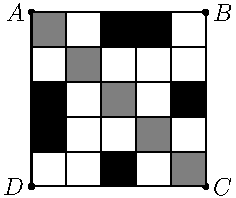
\includegraphics[scale=1.5]{2017.pdf}
    \end{center}
        
        \item Cho $n=2017$. Hãy tìm giá trị nhỏ nhất của $k$ sao cho luôn có một cách gán số $k$-cân đối cho một cách tô màu đối xứng.
\end{enumerate}

    \end{btvn}

    \item \begin{btvn}\vocab{(VNTST 2017).} Có $44$ lỗ khác nhau trên một đường thẳng và $2017$ con kiến. Mỗi con kiến bò ra khỏi một lỗ và bò dọc theo đường thẳng với tốc độ không đổi vào một lỗ khác, sau đó lại vào. Đặt $T$ là tập hợp các khoảnh khắc mà con kiến ra hoặc vào lỗ. Cho biết rằng $|T|\leq 45$ và tốc độ của các con kiến là khác nhau. Chứng minh rằng tồn tại ít nhất hai con kiến không va chạm nhau.
    \end{btvn}

    \item \begin{btvn}\vocab{(VNTST 2017).}
        Đối với mỗi số nguyên $n>0$, một hoán vị $a_1,a_2,\dots ,a_{2n}$ của $1,2,\dots 2n$ được gọi là đẹp nếu với mọi $1\leq i<j \leq 2n$, $a_i+a_{n+i}=2n+1$ và $a_i-a_{i+1}\not \equiv a_j-a_{j+1}$ (mod $2n+1$) (giả sử $a_{2n+1}=a_1$).
        \begin{enumerate}[label=(\alph*)]
            \item Đối với $n=6$, chỉ ra một hoán vị đẹp.
            \item Chứng minh rằng tồn tại một hoán vị đẹp cho mọi $n$.
        \end{enumerate}
    \end{btvn}

    \item \begin{btvn}\vocab{(VMO 2018).}
        Một nhà đầu tư có hai mảnh đất hình chữ nhật có kích thước $120\times 100$.
        \begin{enumerate}[label=(\alph*)]
            \item Trên mảnh đất thứ nhất, cô ấy muốn xây dựng một ngôi nhà có mặt cắt hình chữ nhật kích thước $25\times 35$ và chín chậu hoa tròn với đường kính $5$ bên ngoài ngôi nhà. Chứng minh rằng ngay cả khi vị trí các chậu hoa được chọn ngẫu nhiên trên mảnh đất, diện tích còn lại vẫn đủ để xây dựng ngôi nhà như mong muốn.
            \item Trên mảnh đất thứ hai, cô ấy muốn xây dựng một ao cá đa giác sao cho khoảng cách từ một điểm tùy ý trên mảnh đất, bên ngoài ao cá, đến mép ao gần nhất không quá $5$. Chứng minh rằng chu vi của ao cá không nhỏ hơn $440-20\sqrt{2}$.
        \end{enumerate}
    \end{btvn}

    \item \begin{btvn}\vocab{(VMO 2018).}
        Cho hai số nguyên dương $n$ và $d$, ký hiệu $S_n(d)$ là tập hợp tất cả các $d$-tuples có thứ tự $(x_1,x_2,\dots ,x_d)$ thỏa mãn tất cả các điều kiện sau:
        \begin{enumerate}
            \item $x_i\in {1,2,\dots ,n}$ cho mọi $i\in{1,2,\dots ,d}$
            \item $x_i\ne x_{i+1}$ cho mọi $i\in{1,2,\dots ,d-1}$
            \item Không tồn tại $i,j,k,l\in{1,2,\dots ,d}$ sao cho $i<j<k<l$ và 
            $x_i=x_k,, x_j=x_l$
        \end{enumerate}
        \begin{enumerate}[label=(\alph*)]
        \item Tính $|S_3(5)|$
        \item Chứng minh rằng $|S_n(d)|>0$ nếu và chỉ nếu $d\leq 2n-1$.
        \end{enumerate}
    \end{btvn}

    \item \begin{btvn}\vocab{(VNTST 2018).}
        Đối với mỗi số nguyên dương $m$, một hình chữ nhật có kích thước $m\times 2018$ gồm các ô đơn vị được gọi là ''\textit{hoàn chỉnh}'' nếu các điều kiện sau được thỏa mãn:
        \begin{enumerate}
            \item Trong mỗi ô được viết một số "$0$", một số "$1$" hoặc không gì cả
            \item Đối với mọi chuỗi nhị phân $S$ có độ dài $2018$, ta có thể chọn một hàng và điền vào các ô trống sao cho các số trong hàng đó, nếu đọc từ trái sang phải, tạo ra $S$ (trong trường hợp đặc biệt, nếu một hàng đã đầy và tạo ra $S$ theo cùng một cách thức thì điều kiện ii. này được thỏa mãn).
        \end{enumerate}
        Một hình chữ nhật \textit{hoàn chỉnh} được gọi là \textit{tối thiểu}, nếu ta loại bỏ bất kỳ hàng nào của nó và sau đó nó không còn hoàn chỉnh nữa.
        \begin{enumerate}[label=(\alph*)]
        \item Chứng minh rằng đối với mọi số nguyên dương $k\le 2018$, tồn tại một hình chữ nhật \textit{tối thiểu} có kích thước $2^k\times 2018$ với đúng $k$ cột chứa cả $0$ và $1$.
        \item Một hình chữ nhật \textit{tối thiểu} có kích thước $m\times 2018$ có đúng $k$ cột chứa ít nhất một số $0$ hoặc $1$ và các cột còn lại là trống. Chứng minh rằng $m\le 2^k$.
        \end{enumerate}
    \end{btvn}

    \item \begin{btvn}\vocab{(VNTST 2018).} Trong một lưới vuông $m\times n$, với góc trên bên trái là $A$, có một tuyến đường đi dọc theo cạnh của lưới bắt đầu từ $A$ và ghé qua tất cả các điểm đơn lát (gọi là "nút") đúng một lần và kết thúc cũng tại $A$.
        \begin{enumerate}[label=(\alph*)]
            \item Chứng minh rằng tuyến đường này tồn tại nếu và chỉ nếu ít nhất một trong số $m, n$ là số lẻ.
            \item Nếu một tuyến đường như vậy tồn tại, thì số lượng điểm xoáy ít nhất là bao nhiêu?    
        \end{enumerate}
Một điểm xoáy là một nút khác với $A$ và nếu hai cạnh trên tuyến đường giao nhau tại nút đó là vuông góc.
    \end{btvn}

    \item \begin{btvn}\vocab{(VMO 2019).} 
    Có một số tờ giấy kích thước $5\times 5$ với hai mặt được chia thành các ô vuông đơn vị cho cả hai mặt. Mỗi ô trên tờ giấy được sơn bằng một trong $n$ màu sắc, mỗi màu được sử dụng cho một ô, sao cho hai ô ở cùng vị trí trên hai mặt được sơn bằng cùng một màu. Hai tờ giấy được sơn được coi là giống nhau nếu màu của hai ô tương ứng giống nhau. Chứng minh rằng không có nhiều hơn
    \[
        \frac{1}{8}\left(n^{25}+ 4n^{15} + n^{13} + 2n^7\right)
    \]
    mảnh giấy màu đôi một không giống nhau.
    \end{btvn}
        \begin{sol}\textit{(Phạm Bảo)}
            
            Ta có thể hiểu bài toán là đếm số cách tô một tờ giấy $5 \times 5$ bởi $n$ màu sao cho khác nhau qua các phép quay và lật ngược. Thật vậy, ta có thể dùng ý tưởng của bổ đề Burnside để loại bỏ những cấu hình lặp lại. Tuy nhiên, khó khăn ở đây là nếu ta đếm thống thường (quy tắc nhân) rồi dùng Burnside thì có một vấn đề là có những cấu hình bị lặp ít hơn những cấu hình khác. Khi đó, ta phải chia từng trường hợp nhỏ để kiểm soát và cân bằng số lần lặp của từng cấu hình.
            
            Ở đây ta có thể đếm theo quỹ đạo là $D_8$, tức là mỗi cấu hình sẽ lặp lại (tối đa) 8 lần.

            Theo lý thuyết quỹ đạo của khối nhị diện, ta có các trường hợp đếm lặp là $2^3,2^2,2^1,2^2$ lần và quy ước các trường hợp lớn hơn kế thừa số trường hợp nhỏ hơn (tức là nếu lặp $4$ lần cũng có nghĩa là lặp $1$ và $2$ lần).

            \vocabh{Trường hợp 1:} Tổng quát. Theo quy tắc nhân thì ta có $n^{25}$ cách. Gọi những cấu hình ở trường hợp này là $\mathcal{T}$

            Với mỗi cấu hình có khả năng lặp ở $\mathcal{T}$ phải là một cách tô đối xứng. Ta có tổng cộng ba loại đối xứng: theo trục đứng (ngang), trục đường chéo, theo tâm như hình bên dưới, các trục là đường màu đỏ.

           
            Gọi $\mathcal{A},\mathcal{B},\mathcal{C}$ lần lượt là các cách tô màu đối xứng theo trục đứng, đường chéo và tâm.
            \begin{center}
                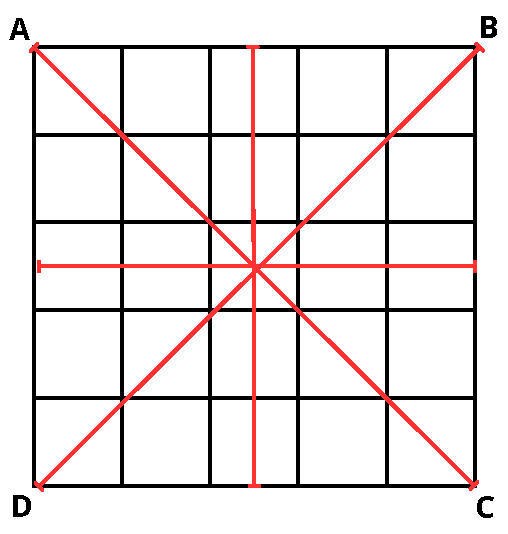
\includegraphics[scale=0.57]{ex1.pdf}
            \end{center}
            \vocabh{Trường hợp 2: }Xét các cấu hình được đếm $4$ lần ở $\mathcal{T}$, khi đó những cấu hình này phải là $\mathcal{A}$ hoặc $\mathcal{B}$. Ví dụ như với trục ngang thì ta có thể tô trục bằng $5$ màu và mỗi bên bằng $10$ màu, tức là cần $15$ màu (có thể trùng nhau).
            \begin{center}
                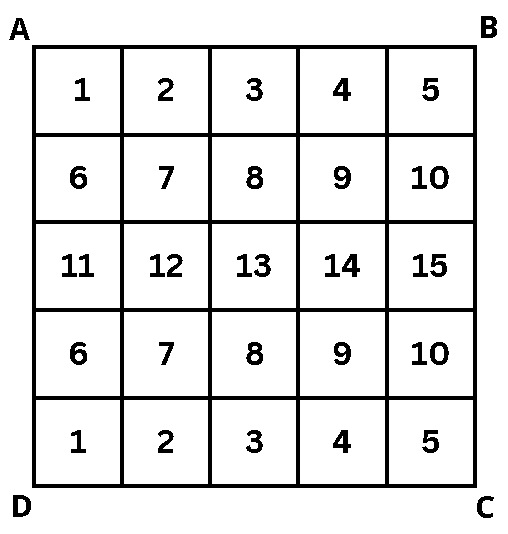
\includegraphics[scale=0.57]{trucngang.pdf}
            \end{center}
            Đối với trục đứng thì bản chất là quay $90^{\circ}$ nên ta được $|\mathcal{A}| = 2n^{15}$. Mặt khác, rõ ràng $f: \mathcal{A} \to \mathcal{B}$ là một song ánh, khi ta cho các số nằm trên trục ngang hoặc dọc lên đường chéo, và mỗi bên đều chứa 10 số, tức là qua phép quay $45^{\circ}$ và ngược lại. Khi đó ta được $|\mathcal{A}|_{TH2} + |\mathcal{B}|_{TH2} = 4n^{15}$.

            \vocabh{Trường hợp 3: }Xét các cấu hình được đếm $2$ lần ở $\mathcal{T}$. Khi này một cách đếm thỏa mãn là bao hàm những cấu hình đối xứng qua cả hai trục ngang-dọc hoặc $AC$-$BD$. Tiến hành tương tự, ta chỉ có thể tô hai trục bằng $3$ màu. Khi đó sẽ chia thành $4$ phần $2\times2$, tô $4$ ô này bằng $4$ màu khác nhau. Ta được tổng cộng $7$ màu. Tương tự cho trục chéo, ta được $|\mathcal{A}|_{TH3} + |\mathcal{B}|_{TH3} = 2n^{7}$.
            \begin{center}
                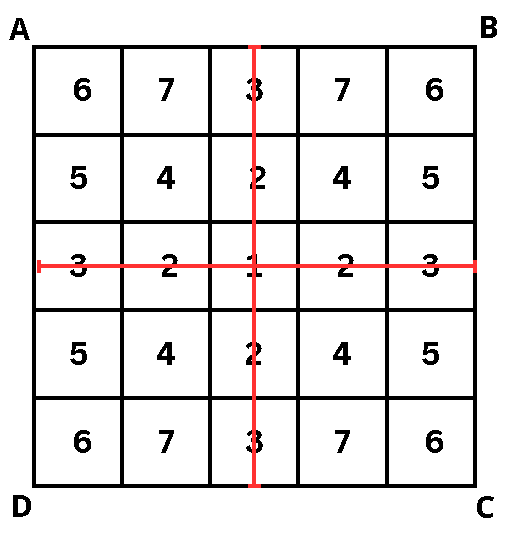
\includegraphics[scale=0.57]{+.pdf}
            \end{center}
            \vocabh{Trường hợp 4: }Xét các cấu hình chỉ lặp lại 1 lần trong $\mathcal{T}$ và cả các kiểu đối xứng không phải trục. Rõ ràng ta phải tính $|\mathcal{C}|$ vì $\mathcal{A} \cap \mathcal{B} \subset \mathcal{C}$. Thật vậy, chọn ô giữa làm tâm, thì khi đó ta được $12$ cặp điểm và ảnh đối xứng của nó, tức là có thể dùng $13$ màu bất kì, ta được $|\mathcal{C}| = n^{13}$.
            \begin{center}
                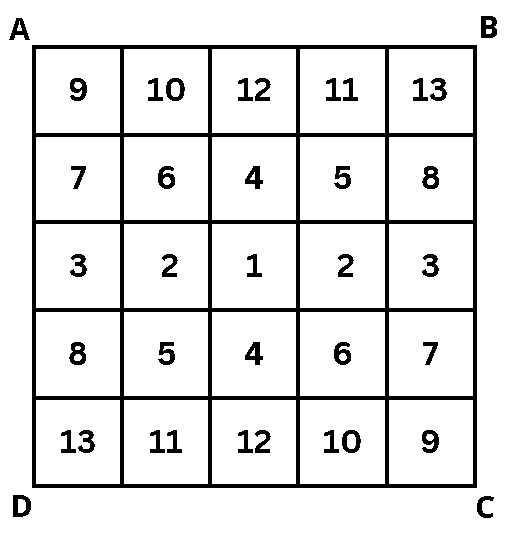
\includegraphics[scale=0.57]{tam.pdf}
            \end{center}

            Cộng tất cả các trường hợp trên lại và áp dụng bổ đề Burnside, ta được tổng số các tô không đối xứng là 
            \[
            S = \frac{1}{8} \left(n^{25} + 4n^{15} + n^{13} + 2n^7\right)
            \]
        \end{sol}
    \item \begin{btvn}\vocab{(VNTST 2019).} Trong một quốc gia có $n\geq 2$ thành phố. Bất kỳ hai thành phố nào cũng có đúng một đường hàng không hai chiều. Chính phủ muốn cấp giấy phép cho một số hãng hàng không để chịu trách nhiệm với các đường hàng không này với các điều kiện sau:
        \begin{enumerate}
            \item Mỗi đường hàng không chỉ có thể được cấp giấy phép cho đúng một hãng hàng không.
            \item Bằng cách chọn một hãng hàng không bất kỳ, chúng ta có thể di chuyển từ một thành phố đến bất kỳ thành phố nào khác, chỉ sử dụng các chuyến bay từ hãng hàng không này.
        \end{enumerate}
        Số lượng tối đa các hãng hàng không mà chính phủ có thể cấp giấy phép để đáp ứng tất cả các điều kiện này là bao nhiêu?
    \end{btvn}

    \item \begin{btvn}\vocab{(VMO 2020).}
        Cho một số nguyên dương $n>1$. Đặt $T$ là một tập chứa tất cả các tập hợp có thứ tự $(x;y;z)$ sao cho $x,y,z$ đều là các số nguyên dương phân biệt và $1\leq x,y,z\leq 2n$. Ngoài ra, một tập $A$ chứa các tập hợp có thứ tự $(u;v)$ được gọi là "kết nối" với $T$ nếu với mọi $(x;y;z)\in T$ thì $\{(x;y),(x;z),(y;z)\} \cap A \neq \varnothing$.
        \begin{enumerate}[label=(\alph*)]
            \item Tìm số phần tử của tập $T$.
            \item Chứng minh rằng tồn tại một tập ''kết nối'' với $T$ có đúng $2n(n-1)$ phần tử.
            \item Chứng minh rằng mọi tập ''kết nối'' với $T$ có ít nhất $2n(n-1)$ phần tử.
        \end{enumerate}

    \end{btvn}

    \item \begin{btvn}\vocab{(VNTST 2020).}
    Cho $n$ là một số nguyên dương, có $4n$ đội tham gia một giải bóng đá. Trong mỗi vòng đấu, chúng ta sẽ chia $4n$ đội thành $2n$ cặp, và mỗi cặp đội sẽ thi đấu cùng một lúc. Sau giải đấu, được biết rằng mỗi cặp đội đã thi đấu tối đa một trận. Tìm số nguyên dương nhỏ nhất $a$, sao cho chúng ta có thể sắp xếp một lịch thi đấu thỏa mãn các điều kiện trên, và nếu chúng ta thêm một vòng đấu nữa, luôn có một cặp đội đã thi đấu trận đấu.
    \end{btvn}

    \item \begin{btvn}\vocab{(VNTST 2020).} Hãy giả sử $n$ là một số nguyên dương. Trên một bảng có kích thước $(2n+1)\times (2n+1)$, mỗi ô được tô màu trắng hoặc đen. Trong mỗi hàng và mỗi cột, nếu số lượng ô màu trắng nhỏ hơn số lượng ô màu đen, chúng ta sẽ đánh dấu tất cả các ô màu trắng. Nếu số lượng ô màu trắng lớn hơn số lượng ô màu đen, chúng ta sẽ đánh dấu tất cả các ô màu đen. Đặt $a$ là số lượng ô màu đen, và $b$ là số lượng ô màu trắng, $c$ là số lượng ô được đánh dấu.

        Ví dụ đối với bảng $3\times 3$, $a=3$, $b=6$, $c=4$.
        \begin{center}
            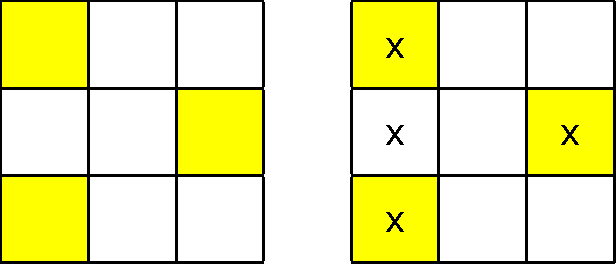
\includegraphics[scale=0.5]{x.pdf}
        \end{center}
        Chứng minh rằng bất kể tình huống tô màu ban đầu như thế nào, luôn có $c\geq\frac{1}{2}\min\{a,b\}$.
    \end{btvn}

    \item \begin{btvn}\vocab{(VMO 2021).}
    Một học sinh chia tất cả $30$ viên bi vào $5$ hộp được đánh số $1, 2, 3, 4, 5$ (sau khi được chia, có thể có một hộp không có viên bi).
    \begin{enumerate}[label=(\alph*)]
        \item Có bao nhiêu cách để chia các viên bi vào các hộp (các cách chia khác nhau nếu có một hộp có số bi khác nhau)?
        \item Sau khi chia, học sinh sẽ sơn các viên bi đó bằng một số màu (mỗi màu sơn được cho nhiều viên bi, một màu có thể được sơn cho nhiều viên bi), sao cho không có $2$ viên bi trong cùng một hộp có màu giống nhau và từ bất kỳ $2$ hộp nào cũng không thể chọn $8$ viên bi đã được sơn bằng $4$ màu. Chứng minh rằng đối với mỗi cách chia, học sinh phải sử dụng ít nhất $10$ màu để sơn các viên bi.
        \item Hãy chỉ ra một cách chia sao cho với chính xác $10$ màu, học sinh có thể sơn các viên bi sao cho thỏa mãn các điều kiện trong câu b).
    \end{enumerate}
    \end{btvn}

    \item \begin{btvn}\vocab{(VNTST 2021).} Trên một bảng gồm $2021 \times 2021$ ô vuông, chọn ra $k$ ô vuông đơn vị sao cho mỗi ô vuông được chọn có chung đỉnh với tối đa $1$ ô vuông khác được chọn. Xác định giá trị lớn nhất của $k$.
    \end{btvn}

    \item \begin{btvn}\vocab{(VMO 2022).}
        Cho 4 viên xúc xắc đồng chất. Ký hiệu $x_i (1\le x_i \le 6)$ là số chấm trên một mặt xuất hiện trên viên xúc xắc thứ $i$ $(1\le i \le 4)$.
        \begin{enumerate}[label=(\alph*)]
            \item Tìm các bộ số $(x_1,x_2,x_3,x_4)$
            \item Tìm xác suất để có một số $x_j$ sao cho $x_j$ bằng tổng của 3 số còn lại.
            \item Tìm xác suất để chúng ta có thể chia $x_1,x_2,x_3,x_4$ thành 2 nhóm có tổng bằng nhau.
        \end{enumerate}
    \end{btvn}

    \item \begin{btvn}\vocab{(VNTST 2022).} Cho một đa diện lồi có 2022 mặt. Trong 3 mặt bất kỳ, đã có các số là $26$, $4$ và $2022$ (mỗi mặt chứa 1 số). Người ta muốn điền vào mỗi mặt còn lại một số thực là trung bình cộng của các số trong các mặt có cạnh chung với mặt đó. Chứng minh rằng chỉ có một cách để điền tất cả các số trong đa diện đó.
    \end{btvn}

    \item \begin{btvn}\vocab{(VNTST 2022).} Cho một tập hợp $A=\{1;2;...;4044\}$. Người ta tô màu $2022$ số trong đó bằng màu trắng và các số còn lại bằng màu đen. Với mỗi $i\in A$, gọi số quan trọng của $i$ là số lượng tất cả các số trắng nhỏ hơn $i$ và các số đen lớn hơn $i$. Với mọi số tự nhiên $m$, hãy tìm tất cả các số nguyên dương $k$ mà tồn tại một cách tô màu các số sao cho có được $k$ số quan trọng bằng $m$.

    \end{btvn}

    \item \begin{btvn}\vocab{(VMO 2023).}
        Có $n \geq 2$ lớp học được tổ chức thành $m \geq 1$ nhóm ngoại khóa cho sinh viên. Mỗi lớp học có sinh viên tham gia ít nhất một nhóm ngoại khóa. Mỗi nhóm ngoại khóa có chính xác $a$ lớp mà các sinh viên trong nhóm này tham gia. Đối với bất kỳ hai nhóm ngoại khóa nào, không có nhiều hơn $b$ lớp với sinh viên tham gia cả hai nhóm đồng thời.
        \begin{enumerate}[label=(\alph*)]
            \item Tìm $m$ khi $n = 8, a = 4 , b = 1$.
            \item Chứng minh rằng $n \geq 20$ khi $m = 6 , a = 10 , b = 4$.
            \item Tìm giá trị nhỏ nhất của $n$ khi $m = 20 , a = 4 , b = 1$.
        \end{enumerate}
    \end{btvn}

    \item \begin{btvn}\vocab{(VNTST 2023).}
    Một trường học có hai lớp học $A$ và $B$ lần lượt có $m$ và $n$ học sinh. Các học sinh của hai lớp học ngồi thành một vòng tròn. Sau đó, mỗi học sinh được tặng một số kẹo bằng số học sinh liên tiếp ngồi bên trái của anh ta đến từ lớp của anh ta. Sau khi phân phát kẹo, giáo viên quyết định nhóm các học sinh sao cho trong mỗi nhóm, tất cả các học sinh nhận được cùng một số lượng kẹo, và bất kỳ hai học sinh nào từ hai nhóm khác nhau đều phải nhận số lượng kẹo khác nhau.
    \begin{enumerate}[label=(\alph*)]
        \item Số học sinh tối đa mà một nhóm có thể có là bao nhiêu?
        \item Loại trừ nhóm mà mỗi học sinh không nhận được kẹo, số học sinh tối đa mà một nhóm có thể có là bao nhiêu?
    \end{enumerate}
    \end{btvn}

    \item \begin{btvn}\vocab{(VNTST 2023).} Cho $n \geq 3$ là một số nguyên và $S$ là một tập hợp gồm $n$ phần tử. Xác định số nguyên lớn nhất $k_n$ sao cho: đối với mỗi cách chọn $k_n$ $3-$phần tử của $S$, tồn tại một cách tô màu các phần tử của $S$ bằng hai màu sao cho không có phần tử nào trong các $3-$phần tử được chọn là đơn sắc.
    \end{btvn}

    \item \begin{btvn}\vocab{(VMO 2024).}
    Cho $k$ viên bi được đặt lên các ô của một lưới $2024 \times 2024$ sao cho mỗi ô có tối đa một viên bi và không có hai viên bi nào được đặt trên hai ô kề nhau (hai ô kề nhau được xác định là các ô có cạnh chung).
    \begin{enumerate}[label=(\alph*)]
        \item Giả sử $k=2024$. Tìm cách đặt các viên bi sao cho mỗi ô có tối đa một viên bi và không có hai viên bi nào được đặt trên hai ô kề nhau (hai ô kề nhau được xác định là các ô có cạnh chung).
        \item Xác định giá trị lớn nhất của $k$ sao cho đối với tất cả các sắp xếp của $k$ viên bi thỏa mãn các điều kiện trên, chúng ta có thể di chuyển một trong những viên bi đã đặt lên một trong các ô kề cạnh của nó và sắp xếp mới vẫn thỏa mãn các điều kiện trên.
    \end{enumerate}
    \end{btvn}

    \item \begin{btvn}\vocab{(VMO 2024).}
        Trong không gian, có một đa diện lồi $D$ sao cho đối với mỗi đỉnh của $D$, có một số lẻ cạnh đi qua đỉnh đó. Chúng ta chọn một mặt $F$ của $D$ sau đó gán mỗi cạnh của $D$ một số nguyên dương sao cho đối với tất cả các mặt của $D$ khác với $F$, tổng các số được gán trên các cạnh của mặt đó là một số nguyên dương chia hết cho $2024$. Chứng minh rằng tổng các số được gán trên các cạnh của $F$ cũng là một số nguyên dương chia hết cho $2024$.
    \end{btvn}

    \item \begin{btvn}\vocab{(VNTST 2024).} Trong một khu vườn có các ô vuông $2024\times 2024$, người ta trồng ba loại hoa: hoa hồng, hoa cúc và hoa lan. Người ta muốn trồng hoa sao cho các điều kiện sau được thỏa mãn:
        \begin{enumerate}
            \item Mỗi ô được trồng tối đa một loại hoa. Một số ô có thể để trống và không trồng hoa.
            \item Đối với mỗi ô được trồng $A$, có đúng $3$ ô khác được trồng trong cùng một cột hoặc hàng sao cho ba ô đó được trồng với các loại hoa khác nhau so với ô $A$.
            \item Mỗi loại hoa được trồng ít nhất trong $1$ ô.
        \end{enumerate}
        Số lớn nhất của các ô có thể được trồng hoa là bao nhiêu?
    \end{btvn}
    \item \begin{btvn}\vocab{(IMOSL 2010 C1).}
        Trong một buổi hòa nhạc, 20 ca sĩ sẽ biểu diễn. Đối với mỗi ca sĩ, có một nhóm (có thể trống) các ca sĩ khác để anh ấy muốn biểu diễn muộn hơn tất cả các ca sĩ từ bộ đó. Có thể xảy ra rằng có chính xác 2010 đơn đặt hàng của các ca sĩ để tất cả mong muốn của họ được thỏa mãn?
    \end{btvn}
    \item \begin{btvn}\vocab{(IMOSL 2010 C2).}
        Trên một vài hành tinh, có $2^n$ quốc gia $(n \geq 4)$. Mỗi quốc gia có một lá cờ rộng $n$ đơn vị và cao một đơn vị gồm có $n$ ô vuông $1\times 1$, mỗi ô có thể có màu xanh hoặc vàng. Không có hai quốc gia nào có cùng lá cờ. Chúng ta nói rằng một tập hợp $n$ lá cờ là đa dạng nếu các lá cờ đó có thể sắp xếp thành $n \times n$ ô vuông sao cho $n$ ô vuông trên đường chéo chính có cùng màu. Xác định giá trị nhỏ nhất của $m$ sao cho mới mọi $m$ là cờ phân biệt, luôn tồn tại $n$ lá cờ tạo nên một tập đa dạng.
    \end{btvn}
    \item \begin{btvn}\vocab{(IMOSL 2010 C3).}
        2500 quân vua được đặt trên bàn cờ $100 \times 100$ sao cho
        \begin{enumerate}
            \item Không vị vua nào có thể bắt được bất kỳ vị vua nào khác (tức là không có hai vị vua nào được đặt trong hai ô vuông có chung một đỉnh)
            \item Mỗi hàng và mỗi cột chứa chính xác 25 vị vua.
        \end{enumerate}
        Tìm số lượng sắp xếp như vậy. (Hai cách sắp xếp khác nhau bằng cách xoay hoặc đối xứng được cho là khác nhau.)

    \end{btvn}
    
    \item \begin{btvn}\vocab{(IMO/IMOSL 2010 C4).}
        Mỗi hộp trong số sáu hộp $B_1$, $B_2$, $B_3$, $B_4$, $B_5$, $B_6$ ban đầu chứa một đồng xu. Ta có các hoạt động như sau:

        \begin{itemize}[label=-]
            \item \vocab{Loại 1:} Chọn một hộp không trống $B_j$, $1\leq j \leq 5$, loại bỏ một đồng xu khỏi $B_j$ và thêm hai đồng xu vào $B_{j+1}$;
            \item \vocab{Loại 2:} Chọn một hộp không trống $B_k$, $1\leq k \leq 4$, loại bỏ một đồng xu khỏi $B_k$ và hoán đổi số đồng xu (có thể trống) của các hộp $B_{k+1}$ và $ B_{k+2}$.

        \end{itemize}
        Xác định xem có tồn tại một chuỗi hữu hạn các phép toán thuộc các loại trên hay không, sao cho năm hộp $B_1$, $B_2$, $B_3$, $B_4$, $B_5$ trở nên trống rỗng, trong khi hộp $B_6$ chứa chính xác $2010^ {2010^{2010}}$ xu.
    \end{btvn}

    \item \begin{btvn}\vocab{(IMOSL 2010 C5).}
        Có $n \geq 4$ người chơi đã tham gia một giải quần vợt. Hai người chơi bất kỳ đã chơi đúng một ván và không có ván hòa. Chúng ta gọi một nhóm gồm bốn người chơi là tệ nếu một người chơi bị đánh bại bởi ba người chơi khác và mỗi người trong số ba người chơi này thắng một ván và thua một ván khác với nhau. Giả sử không có nhóm nào tệ trong giải đấu này. Gọi $w_i$ và $l_i$ lần lượt là số lần thắng và thua của người chơi thứ $i$. Chứng minh rằng\[\sum^n_{i=1} \left(w_i - l_i\right)^3 \geq 0.\]
    \end{btvn}
    \item \begin{btvn}\vocab{(IMOSL 2010 C6).}
        Cho một số nguyên dương $k$ và hai số nguyên khác nhau $b > w > 1.$ Có hai chuỗi ngọc trai, một chuỗi ngọc trai đen $b$ và một chuỗi ngọc trai trắng $w$. Độ dài của sợi dây chính là số hạt ngọc trên đó. Người ta cắt những sợi dây này theo một số bước theo các quy tắc sau. Trong mỗi bước:
        \begin{enumerate}
            \item Các chuỗi được sắp xếp theo độ dài theo thứ tự không tăng. Nếu có một số chuỗi có độ dài bằng nhau thì chuỗi trắng đứng trước chuỗi đen. Sau đó $k$ những viên đầu tiên (nếu chúng bao gồm nhiều hơn một viên ngọc) được chọn; nếu có ít hơn $k$ chuỗi dài hơn 1 thì người ta sẽ chọn tất cả các chuỗi đó.
            \item Tiếp theo, người ta cắt mỗi sợi dây đã chọn thành hai đoạn có độ dài khác nhau nhiều nhất là một. (Ví dụ: nếu có các chuỗi ngọc trai đen $5, 4, 4, 2$, chuỗi ngọc trai trắng $8, 4, 3$ và $k = 4,$ thì chuỗi 8 trắng, 5 đen, 4 trắng và 4 viên ngọc trai đen được cắt thành các phần tương ứng $(4,4), (3,2), (2,2)$ và $(2,2)$.) Quá trình dừng ngay sau bước khi một viên ngọc trai trắng đầu tiên được tách ra. ngọc xuất hiện.
        \end{enumerate}
Chứng minh rằng ở bước này vẫn tồn tại một chuỗi gồm ít nhất hai viên ngọc đen.
    \end{btvn}
    \item \begin{btvn}\vocab{(IMOSL 2010 C7).}
        Cho $P_1, \ldots , P_s$ là cấp số cộng của các số nguyên, thỏa mãn các điều kiện sau:
        \begin{enumerate}
            \item Mỗi số nguyên thuộc về ít nhất một trong số chúng.
            \item Mỗi cấp số chứa một số không thuộc cấp số khác.
        \end{enumerate} 
        
        Ký hiệu $n$ là bội số chung nhỏ nhất của các cấp số nhân này phân tích thành thừa số nguyên tố $n=p_1^{\alpha_1} \cdots p_k^{\alpha_k}$. Chứng minh rằng \[s \geq 1 + \sum^k_{i=1} \alpha_i (p_i - 1).\]
    \end{btvn}

    \item \begin{btvn}\vocab{(IMOSL 2011 C1).} Cho $n > 0$ là một số nguyên. Chúng ta có một cái cân và $n$ quả cân trọng lượng $2^0, 2^1, \cdots, 2^{n-1}$. Chúng ta đặt từng quả cân lên cân sao cho đĩa bên phải không bao giờ nặng hơn đĩa bên trái. Ở mỗi bước, chúng ta chọn một trong các quả cân chưa được đặt lên cân và đặt nó lên đĩa bên trái hoặc đĩa bên phải cho đến khi tất cả các quả cân đã được đặt xong. Hãy xác định số cách có thể thực hiện được điều này.
    \end{btvn}

    \item \begin{btvn}\vocab{(IMOSL 2011 C2).}
        Giả sử rằng sinh viên $1000$ đang đứng thành một vòng tròn. Chứng minh rằng tồn tại một số nguyên $k$ với $100 \leq k \leq 300$ sao cho trong vòng tròn này tồn tại một nhóm liền kề gồm $2k$ học sinh, trong đó nửa đầu chứa số nữ sinh bằng nửa sau.
    \end{btvn}

    \item \begin{btvn}\vocab{(IMO/IMOSL 2011 C2).}
        Cho $\mathcal{S}$ là tập hợp hữu hạn có ít nhất 2 điểm trong mặt phẳng. Giả sử rằng không có 3 điểm nào thẳng hàng. Một \textit{cối xay gió} là một quá trình bằng đầu từ đường thẳng $\ell$ qua một điểm $P \in \mathcal{S}$. Đường thẳng quay theo chiều kim đồng hồ quanh trục quay $P$ đến khi đường thẳng gặp một vài điểm khác thuộc $\mathcal{S}$. Quá trình này diễn ra một cách liên tục. Chứng minh rằng chúng ta có thể chọn một điểm $P$ thuộc $\mathcal{S}$ và một đường thẳng $\ell$ đi qua $P$ sao cho \textit{cối xây gió} sẽ sử dụng mọi điểm thuộc $\mathcal{S}$ làm trục lặp lại một cách vô hạn.
    \end{btvn}

    \item \begin{btvn}\vocab{(IMOSL 2011 C4).}
        Xác định số nguyên dương lớn nhất $k$ thỏa mãn tính chất sau: Tập hợp các số nguyên dương có thể được phân chia thành $k$ tập con $A_1, A_2, \ldots, A_k$ sao cho mọi số nguyên $n \geq 15$ và tất cả $i \in \{1, 2, \ldots, k\}$ tồn tại hai phần tử riêng biệt của $A_i$ có tổng là $n$.
    \end{btvn}

    \item \begin{btvn}\vocab{(IMOSL 2011 C5).}
        Cho số nguyên dương $m$, và xét bảng ô vuông $m\times m$ có các ô vuông đơn vị. Tại một vài ô vuông đơn vị có một con kiến. Ở thời điểm $0$, mỗi con kiếm di chuyển với tốc độ là $1$ song song với một vài cạnh của bảng. Khi hai con kiến di chuyển ngược chiều gặp nhau, chúng đều quay đầu $90^{\circ}$ theo chiều kim đồng hồ và tiếp tục di chuyển với tốc độ $1$. Khi có nhiều hơn 2 con kiến gặp nhau, hoặc hai con kiến di chuyển vuông góc gặp nhau, chúng sẽ tiếp tục di chuyển theo hướng y hệt trước đó. Khi một con kiến di chuyển đến cạnh của bảng thì nó sẽ bị loại và không thể xuất hiện lại được nữa. 

        Xem xét tất cả các vị trí bắt đầu có thể, xác định thời điểm muộn nhất có thể mà tại đó con kiến cuối cùng rơi khỏi bàn cờ, hoặc chứng minh rằng thời điểm đó không nhất thiết phải tồn tại.

    \end{btvn}

    \item \begin{btvn}\vocab{(IMOSL 2011 C6).}
    Cho $n$ là một số nguyên dương và $W = \ldots x_{-1}x_0x_1x_2 \ldots$ là một từ tuần hoàn vô hạn, chỉ bao gồm các chữ cái $a$ hoặc $b$. Giả sử độ dài của từ $N$ lớn hơn $W$ chữ cái $2^n$.

    Một từ hữu hạn $U$ được cho là xuất hiện trong $W$ nếu tồn tại các chỉ số $k \leq \ell$ sao cho $U=x_k x_{k+1} \ldots x_{\ell}$. Một từ hữu hạn $U$ được gọi là phổ biến nếu bốn từ $Ua$, $Ub$, $aU$ và $bU$ đều xuất hiện trong $W$. Chứng minh rằng có ít nhất $n$ các từ phổ biến khác rỗng có mặt khắp nơi.
    \end{btvn}

    \item \begin{btvn}\vocab{(IMOSL 2011 C7).}
    Trên một bàn vuông có các ô $2011 \times 2011$ đặt một số lượng hữu hạn khăn ăn bao phủ một hình vuông có kích thước các ô $52$ x $52$. Trong mỗi ô, viết số lượng khăn ăn che nó và ghi lại số $k$ tối đa của các ô mà tất cả đều chứa cùng một số khác 0. Xem xét tất cả các cấu hình khăn ăn có thể có, giá trị lớn nhất của $k$ là bao nhiêu?
    \end{btvn}
    \item \begin{btvn}\vocab{(IMOSL 2012 C1).}
        Một vài số nguyên dương được viết thành một hàng. Liên tục lặp lại, Alice chọn hai số liền kề $x$ và $y$ sao cho $x>y$ và $x$ nằm ở bên trái của $y$, và thay thế cặp $(x,y)$ bằng $(y) +1,x)$ hoặc $(x-1,x)$. Chứng minh rằng cô ấy chỉ có thể thực hiện hữu hạn nhiều lần lặp như vậy.
    \end{btvn}

    \item \begin{btvn}\vocab{(IMOSL 2012 C2).}
        Cho $n \geq 1$ là một số nguyên. Số lượng tối đa các cặp phần tử rời nhau của tập $\{ 1,2,\ldots , n \}$ sao cho tổng của các cặp khác nhau là các số nguyên khác nhau không vượt quá $n$?
    \end{btvn}

    \item \begin{btvn}\vocab{(IMOSL 2012 C3).}
    Trong một bảng vuông $999 \times 999$, một số ô có màu trắng và các ô còn lại có màu đỏ. Gọi $T$ là số bộ ba $(C_1,C_2,C_3)$ của các ô, hai ô đầu tiên trong cùng một hàng và hai ô cuối cùng trong cùng một cột, với $C_1,C_3$ màu trắng và $C_2$ màu đỏ. Tìm giá trị lớn nhất $T$ có thể đạt được.
    \end{btvn}

    \item \begin{btvn}\vocab{(IMOSL 2012 C4).}
    Người chơi $A$ và $B$ chơi một trò chơi với các đồng xu $N \geq 2012$ và các hộp $2012$ được sắp xếp xung quanh một vòng tròn. Ban đầu $A$ phân phối các đồng xu vào các hộp sao cho có ít nhất đồng xu $1$ trong mỗi hộp. Sau đó hai người thực hiện các nước đi theo thứ tự $B,A,B,A,\ldots $ theo quy tắc sau:
    \begin{enumerate}
        \item Mỗi lần di chuyển $B$ của anh ta sẽ chuyển đồng xu $1$ từ mỗi hộp sang hộp liền kề.
        \item Trong mỗi nước đi của cô ấy, $A$ chọn một số đồng xu không liên quan đến nước đi trước đó của $B$ và nằm trong các hộp khác nhau. Cô ấy chuyển từng đồng xu sang một hộp bên cạnh.
    \end{enumerate}
    Mục tiêu của người chơi $A$ là đảm bảo có ít nhất đồng xu $1$ trong mỗi ô sau mỗi nước đi của mình, bất kể $B$ chơi như thế nào và bao nhiêu nước đi được thực hiện. Tìm ít nhất $N$ để cô ấy có thể thành công.
    \end{btvn}
    
    \item \begin{btvn}\vocab{(IMOSL 2012 C5).}
        Cho một bảng ô vuông $3n \times 3n$ có các cột và hàng được đánh dấu từ $1$ đến $3n$. Mỗi ô vuông $(x,y)$ với $1 \leq x,y \leq 3n$ được tô màu xanh, đỏ hoặc vàng dựa trên tổng $x + y$ theo module 3 lần lượt là 0,1,2. Một tấm thẻ có màu xanh, đỏ hoặc vàng được đặt lên từng ô vuông.
        
        
        Giả sử rằng người ta có thể hoán vị các tấm thẻ sao cho mỗi tấm thẻ được di chuyển với khoảng cách lớn nhất là $d$ so với vị trí ban đầu, thẻ xanh được thay thế bởi thẻ đỏ, thẻ được thay thế bởi thẻ vàng và thẻ vàng được thay thế bởi thẻ xanh. Chứng minh rằng có thể hoán vị các thẻ sao cho mỗi thẻ được di chuyển với một khoảng cách tối đa là $d + 2$ so với vị trí ban đầu của nó và mỗi ô vuông chứa thẻ cùng màu với màu của nó.
    \end{btvn}

    \item \begin{btvn}\vocab{(IMO/IMOSL 2012 C6).}
        Trò chơi đoán của kẻ nói dối là trò chơi được chơi giữa hai người chơi $A$ và $B$. Luật chơi phụ thuộc vào hai số nguyên dương $k$ và $n$ mà cả hai người chơi đều biết trước.
    
        Khi bắt đầu trò chơi $A$ chọn các số nguyên $x$ và $n$ với $1 \le x \le n.$ Người chơi $A$ giữ bí mật về $x$ và nói thật về $n$ cho người chơi $B$. Người chơi $B$ bây giờ cố gắng lấy thông tin về $x$ bằng cách hỏi người chơi $A$ các câu hỏi như sau: 
    
        - Mỗi câu hỏi bao gồm $B$ chỉ định một tập hợp $S$ số nguyên dương tùy ý (có thể là một câu hỏi được chỉ định trong một số câu hỏi trước đó), và hỏi $A$ liệu $x$ có thuộc về $S$ hay không. 
            
        Người chơi $B$ có thể hỏi bao nhiêu câu hỏi tùy thích. Sau mỗi câu hỏi, người chơi $A$ phải trả lời ngay có hoặc không, nhưng được phép nói dối bao nhiêu lần tùy thích; hạn chế duy nhất là, trong số các câu trả lời $k+1$ liên tiếp, ít nhất một câu trả lời phải trung thực.
            
        Sau khi $B$ hỏi bao nhiêu câu hỏi tùy thích, anh ta phải chỉ định một tập $X$ gồm nhiều nhất $n$ số nguyên dương. Nếu $x$ thuộc về $X$ thì $B$ thắng; nếu không, anh ta sẽ thua. Chứng minh rằng:
        \begin{enumerate}[label=(\alph*)]
            \item Nếu $n \ge 2^k,$ thì $B$ có thể đảm bảo thắng.
            \item Với tất cả $k$ đủ lớn, tồn tại một số nguyên $n \ge (1,99)^k$ sao cho $B$ không thể đảm bảo thắng.
        \end{enumerate}
    \end{btvn}


    \item \begin{btvn}\vocab{(IMOSL 2012 C7).}
        Cho $2^{500}$ điểm nằm trên một đường tròn được đánh theo số thứ tự $1,2,\dots,2^{500}$. Chứng minh rằng có thể chọn ra $100$ cặp điểm rời nhau để nối một số điểm trong số này sao cho $100$ tổng của các cặp số tại điểm cuối của dây cung đã chọn là bằng nhau.
    \end{btvn}

    \item\begin{btvn}\vocab{(IMOSL 2013 C1).} Cho $n$ là một số nguyên dương. Tìm số nguyên nhỏ nhất $k$ có tính chất sau; Cho bất kỳ số thực $a_1 , \cdots , a_d $ sao cho $a_1 + a_2 + \cdots + a_d = n$ và $0 \le a_i \le 1$ với $i=1,2,\cdots ,d$, nó có thể phân chia các số này thành các nhóm $k$ (một số có thể trống) sao cho tổng các số trong mỗi nhóm nhiều nhất là $1$.
    \end{btvn}
    
    \item \begin{btvn}\vocab{(IMO/IMOSL 2013 C2).}
        Một cấu hình gồm các điểm $4027$ trong mặt phẳng được gọi là Colombia nếu nó bao gồm $2013$ điểm đỏ và $2014$ điểm xanh, và không có ba điểm nào trong cấu hình thẳng hàng. Bằng cách vẽ một số đường, mặt phẳng được chia thành nhiều vùng. Việc sắp xếp các đường là tốt cho cấu hình Colombia nếu hai điều kiện sau được thỏa mãn:
        \begin{enumerate}
            \item Không có đường thẳng nào đi qua bất kỳ điểm nào của hình.
            \item Không có vùng nào chứa điểm có cả hai màu.
        \end{enumerate}
        Tìm giá trị nhỏ nhất của $k$ sao cho với bất kỳ cấu hình Colombia nào có $4027$ điểm , có sự sắp xếp hợp lý cho $k$ đường thẳng.
    \end{btvn}
    
    \item \begin{btvn}\vocab{(IMOSL 2013 C3).}
        Vào một ngày đẹp trời, Thắng đã phát hiện một giống loài mới mà anh gọi là \textit{Kẹo}, anh thương chúng như con của mình. Một số cặp \textit{Kẹo} có thể xích mích với nhau và mỗi \textit{Kẹo} có thể tham gia vào nhiều mối quan hệ xích mích. Thắng ngọt đã tìm ra cách thực hiện hai loại thao tác sau đây với các con của mình, mỗi lần một thao tác.
        \begin{enumerate}
            \item Nếu một \textit{Kẹo} nào đó bị xích mích với một số lẻ các \textit{Kẹo} khác thì Thắng có thể bỏ con.
            \item Vào bất kỳ lúc nào, anh ta có thể nhân đôi toàn bộ  \textit{Kẹo} bằng cách ra album mới để tạo một bản sao $I'$ của mỗi  \textit{Kẹo} $I$. Trong quá trình này, hai bản sao $I'$ và $J'$ trở nên xích mích khi và chỉ khi các \textit{Kẹo} gốc $I$ và $J$ có xích mích nhau, và mỗi bản sao $I'$ trở nên xích mích với  \textit{Kẹo} ban đầu của nó $I $; không có xích mích nào khác xảy ra hoặc Thắng bỏ con tại thời điểm này.
        \end{enumerate}
        Chứng minh rằng Thắng có thể áp dụng một dãy các phép toán như vậy khi ra nhạc để tạo ra một họ \textit{Kẹo}, trong đó không có hai con nào xích mích.
    \end{btvn}

    \item \begin{btvn}\vocab{(IMOSL 2013 C4).}
        Cho $n$ là một số nguyên dương và gọi $A$ là tập con của $\{ 1,\cdots ,n\}$. Một phân hoạch $A$ của $n$ thành $k$ phần là biểu diễn của n dưới dạng tổng $n = a_1 + \cdots + a_k$, trong đó các phần $a_1 , \cdots , a_k $ thuộc về $A$ và không nhất thiết phải khác biệt. Số phần khác nhau trong một phân hoạch như vậy là số phần tử (riêng biệt) trong tập $\{ a_1 , a_2 , \cdots , a_k \} $.
        Chúng ta nói rằng phân hoạch $A$ của $n$ thành các phần $k$ là \textit{tối ưu} nếu không có phân hoạch $A$ của $n$ thành các phần $r$ với $r<k$. Chứng minh rằng mọi phân hoạch $A$-tối ưu của $n$ đều chứa tối đa $\sqrt[3]{6n}$ các phần khác nhau.
    \end{btvn}

    \item \begin{btvn}\vocab{(IMOSL 2013 C5).}
        Cho $r$ là một số nguyên dương và đặt $a_0 , a_1 , \cdots $ là một chuỗi vô hạn các số thực. Giả sử rằng với tất cả các số nguyên không âm $m$ và $s$ đều tồn tại một số nguyên dương $n \in [m+1, m+r]$ sao cho
\[ a_m + a_{m+1} +\cdots +a_{m+s} = a_n + a_{n+1} +\cdots +a_{n+s} \]

        Chứng minh rằng dãy tuần hoàn, tức là tồn tại một số $p \ge 1 $ sao cho $a_{n+p} =a_n $ với mọi $n \ge 0$.
    \end{btvn}
    \item \begin{btvn}\vocab{(IMOSL 2013 C6).} Ở một số quốc gia, một số cặp thành phố được kết nối bằng các chuyến bay hai chiều trực tiếp. Có thể đi từ thành phố này đến thành phố khác bằng một chuỗi các chuyến bay. Khoảng cách giữa hai thành phố được xác định là số chuyến bay cần thiết ít nhất có thể để đi từ thành phố này đến thành phố kia. Người ta biết rằng đối với bất kỳ thành phố nào, có nhiều nhất các thành phố $100$ cách nó đúng ba lần. Chứng minh rằng không có thành phố nào có hơn $2550$ các thành phố khác có khoảng cách chính xác là $4$.
    \end{btvn}
    
    \item \begin{btvn}\vocab{(IMOSL 2013 C7).}
        Cho $n \ge 3$ là một số nguyên và xét một đường tròn có $n + 1$ điểm cách đều nhau được đánh dấu trên đó. Ta gán cho mỗi điểm bởi một trong các nhãn $0, 1, ... , n$ sao cho mỗi nhãn được sử dụng đúng một lần. Hai cách gán nhãn được coi là giống nhau nếu cách này có thể trở thành cách kia theo một phép quay vòng tròn. Một cách gán nhãn được gọi là đẹp nếu với bốn nhãn bất kỳ $a < b < c < d$ với $a + d = b + c$, dây nối các điểm có nhãn $a$ và $d$ không giao nhau với dây nối các điểm có nhãn $b$ và $c$.

        Gọi $M$ là số lượng nhãn đẹp và $N$ là số cặp có thứ tự $(x, y)$ gồm các số nguyên dương sao cho $x + y \le n$ và $\gcd(x, y) = 1$. Chứng minh rằng $M = N + 1.$
    \end{btvn}

    \item \begin{btvn}\vocab{(IMOSL 2013 C8).}
        Người chơi $A$ và $B$ chơi một trò chơi trên trục số thực. Người chơi $A$ có một bình sơn có bốn đơn vị mực đen. Một lượng $p$ của loại mực này đủ để bôi đen một khoảng thực (đóng) có độ dài $p$. Trong mỗi vòng, người chơi $A$ chọn một số nguyên dương $m$ và cung cấp $1/2^m $ đơn vị mực từ hũ. Người chơi $B$ sau đó chọn một số nguyên $k$ và bôi đen khoảng từ $k/2^m$ đến $(k+1)/2^m$ (một số phần của khoảng này có thể đã bị bôi đen trước đó). Mục tiêu của người chơi $A$ là đạt được bôi đen cho đến khi lọ mực hết sạch và khoảng $[0,1]$ không bị đen hoàn toàn.
        Hỏi có tồn tại chiến lược để người chơi $A$ giành chiến thắng trong một số nước đi hữu hạn hay không.
    \end{btvn}
    \item \begin{btvn}\vocab{(IMOSL 2014 C1).} Cho $n$ điểm bên trong hình chữ nhật $R$ sao cho không có hai điểm nào nằm trên một đường thẳng song song với một cạnh của $R$. Hình chữ nhật $R$ sẽ được chia thành các hình chữ nhật nhỏ hơn với các cạnh song song với các cạnh của $R$ sao cho không có hình chữ nhật nào chứa bất kỳ điểm nào trong số các điểm đã cho bên trong nó. Chứng minh rằng chúng ta phải chia $R$ thành ít nhất $n + 1$ hình chữ nhật nhỏ hơn.
    \end{btvn}

    \item \begin{btvn}\vocab{(IMOSL 2014 C2).}
        Chúng ta có những tờ giấy trị giá $2^m$, trên mỗi tờ giấy có ghi số $1$. Chúng ta thực hiện thao tác sau. Ở mỗi bước, chọn hai tờ riêng biệt, nếu các số trên hai tờ là $a$ và $b$ thì ta xóa các số này và viết số $a + b$ lên cả hai tờ. Chứng minh rằng sau $m2^{m -1}$ bước, tổng các số trên tất cả các trang ít nhất là $4^m$.
    \end{btvn}

    \item \begin{btvn}\vocab{(IMOSL 2014 C3).}
        Cho $n \ge 2$ là một số nguyên. Xét một bàn cờ vua $n \times n$ gồm $n^2$ ô đơn vị. Một cấu hình của $n$ quân xe trên bảng này là hòa bình nếu mỗi hàng và mỗi cột chứa đúng một quân xe. Tìm số nguyên dương lớn nhất $k$ sao cho, đối với mỗi cấu hình hòa bình của $n$ quân xe, tồn tại một ô vuông $k \times k$ không chứa quân xe trên bất kỳ ô đơn vị nào trong $k^2$ ô của nó.
    \end{btvn}

    \item \begin{btvn}\vocab{(IMOSL 2014 C4).}
    Giả sử rằng một đa giác mạng tinh thể (được tạo ra bởi các điểm trên lưới ô vuông) $P$ có thể được lát bằng $S$-tetrominoes. Chứng minh rằng cho dù chúng ta lát $P$ bằng cách sử dụng $S$-tetrominoes hay $Z$-tetrominoes như thế nào, chúng ta luôn sử dụng một số chẵn $Z$-tetrominoes.
    \end{btvn}
    \item \begin{btvn}\vocab{(IMO/IMOSL 2014 C5).}
        Một tập hợp các đường trong mặt phẳng được gọi là \textit{tổng quát} nếu không có hai đường nào song song và không có ba đường nào đi qua cùng một điểm. Một tập hợp các đường trong tổng quát cắt mặt phẳng thành các vùng, một số trong số đó có diện tích hữu hạn; chúng ta gọi chúng là các vùng hữu hạn. Chứng minh rằng đối với tất cả các số nguyên dương $n$ đủ lớn, trong bất kỳ tập hợp $n$ đường nào trong \textit{tổng quát}, ta luôn có thể tô màu ít nhất $\sqrt{n}$ đường màu xanh sao cho không có vùng hữu hạn nào có biên hoàn toàn màu xanh.
    Chú ý: Các kết quả với $\sqrt{n}$ thay thế bằng $c\sqrt{n}$ sẽ được điểm tùy thuộc vào giá trị của hằng số $c$.
    \end{btvn}

    \item \begin{btvn}\vocab{(IMOSL 2014 C6).}
        Cho một bộ bài vô hạn, mỗi lá có một số thực trên đó. Đối với mỗi số thực $x$, có đúng một lá bài trong bộ bài có $x$ viết trên đó. Bây giờ hai người chơi rút các tập hợp rời rạc $A$ và $B$ gồm $100$ lá bài mỗi tập từ bộ bài này. Chúng ta muốn định nghĩa một quy tắc để xác định người chiến thắng. Quy tắc này phải thoả mãn các điều kiện sau:
        \begin{enumerate}
            \item Người chiến thắng chỉ phụ thuộc vào thứ tự tương đối của $200$ lá bài: nếu các lá bài được đặt xuống theo thứ tự tăng dần mặt dưới và chúng ta được biết lá bài nào thuộc về người chơi nào, nhưng không biết số nào được viết trên chúng, chúng ta vẫn có thể quyết định người chiến thắng.
            \item Nếu chúng ta viết các phần tử của cả hai tập hợp theo thứ tự tăng dần như $A ={ a_1 , a_2 , \ldots, a_{100} }$ và $B= { b_1 , b_2 , \ldots , b_{100} }$, và $a_i > b_i$ cho mọi $i$, thì $A$ sẽ thắng $B$.
            \item Nếu ba người chơi rút ba tập hợp rời rạc $A, B, C$ từ bộ bài, $A$ thắng $B$ và $B$ thắng $C$ thì $A$ cũng thắng $C$.
        \end{enumerate}
    Có bao nhiêu cách để định nghĩa một quy tắc như vậy? Ở đây, chúng ta xem xét hai quy tắc là khác nhau nếu tồn tại hai tập hợp $A$ và $B$ sao cho $A$ thắng $B$ theo một quy tắc, nhưng $B$ thắng $A$ theo quy tắc khác.
    \end{btvn}

    \item \begin{btvn}\vocab{(IMOSL 2014 C7).}
        Cho $M$ là một tập hợp gồm $n \geq 4$ điểm trong mặt phẳng, không có ba điểm nào thẳng hàng. Ban đầu các điểm này được kết nối bằng $n$ đoạn thẳng sao cho mỗi điểm trong $M$ là điểm cuối của đúng hai đoạn thẳng. Sau đó, ở mỗi bước, người ta có thể chọn hai đoạn thẳng $AB$ và $CD$ có một điểm nội tiếp chung và thay thế chúng bằng các đoạn thẳng $AC$ và $BD$ nếu không có một trong chúng được hiện diện tại thời điểm này. Chứng minh rằng không thể thực hiện $n^3 /4$ hoặc nhiều bước di chuyển như vậy.
    \end{btvn}
    \item \begin{btvn}\vocab{(IMOSL 2014 C8).}
    Một bộ bài gồm $1024$ lá bài. Trên mỗi lá bài, một tập hợp các chữ số thập phân riêng biệt được viết sao cho không có hai tập hợp nào trùng nhau. Hai người chơi lần lượt lấy các lá bài từ bộ bài, mỗi lượt lấy một lá. Sau khi lấy hết bộ bài, mỗi người chơi kiểm tra xem họ có thể vứt đi một trong các lá bài của mình sao cho mỗi chữ số trong số mười chữ số xuất hiện trên một số lẻ các lá bài còn lại của mình hay không. Nếu một người chơi có thể làm điều này nhưng người chơi kia không thể, người có thể làm được sẽ là người chiến thắng; nếu không, sẽ tuyên bố hòa.

    
    Xác định tất cả các nước đi đầu tiên có thể của người chơi đầu tiên để anh ta có chiến lược chiến thắng.
    \end{btvn}

    \item \begin{btvn}\vocab{(IMOSL 2014 C9).}
    Có $n$ hình tròn được vẽ trên một tờ giấy sao cho bất kỳ hai hình tròn nào cũng cắt nhau tại hai điểm, và không có ba hình tròn nào đi qua cùng một điểm. Turbo, con ốc sên, trượt dọc theo các hình tròn theo cách sau. Ban đầu, nó di chuyển trên một trong các hình tròn theo hướng kim đồng hồ. Turbo luôn tiếp tục trượt dọc theo hình tròn hiện tại cho đến khi anh ta đến một điểm giao với một hình tròn khác. Sau đó, anh ta tiếp tục hành trình của mình trên hình tròn mới này và cũng thay đổi hướng di chuyển, tức là từ hướng kim đồng hồ sang hướng ngược lại hoặc ngược lại.
    Giả sử rằng con đường của Turbo hoàn toàn bao phủ tất cả các hình tròn. Chứng minh rằng $n$ phải là số lẻ.
    \end{btvn}
    \item \begin{btvn}\vocab{(IMOSL 2015 C1).}
        Ở Lineland có các thị trấn $n\geq1$, được bố trí dọc theo một con đường chạy từ trái sang phải. Mỗi thị trấn có một máy ủi bên trái (đặt bên trái thị trấn và quay mặt về bên trái) và một máy ủi bên phải (đặt bên phải thị trấn và quay mặt về bên phải). Kích thước của những chiếc máy ủi trị giá 2 tỷ USD là khác nhau. Mỗi khi xe ủi bên trái và bên phải đối đầu nhau, xe ủi lớn hơn sẽ đẩy chiếc nhỏ hơn ra khỏi đường. Mặt khác, máy ủi khá không được bảo vệ ở phía sau; vì vậy, nếu một chiếc máy ủi chạm tới đuôi của một chiếc xe khác, chiếc thứ nhất sẽ đẩy chiếc thứ hai ra khỏi đường, bất kể kích thước của chúng như thế nào.


        Giả sử $A$ và $B$ là hai thị trấn, với $B$ ở bên phải $A$. Chúng ta nói rằng thị trấn $A$ có thể quét sạch thị trấn $B$ nếu xe ủi bên phải của $A$ có thể di chuyển tới $B$ và đẩy tất cả các máy ủi mà nó gặp. Tương tự, thị trấn $B$ có thể quét sạch thị trấn $A$ nếu xe ủi bên trái của $B$ có thể di chuyển tới $A$ đẩy tất cả các máy ủi của tất cả các thị trấn trên đường đi của nó.

        
        Chứng minh rằng có đúng một thị trấn không thể bị một thị trấn nào khác cuốn trôi.
    \end{btvn}
    
    \item \begin{btvn}\vocab{(IMO/IMOSL 2015 C2).}
        Chúng ta nói rằng một tập hợp hữu hạn $\mathcal{S}$ các điểm trong mặt phẳng là \textit{cân bằng} nếu như đối với bất kỳ hai điểm khác nhau $A$ và $B$ trong $\mathcal{S}$, có một điểm $C$ trong $\mathcal{S}$ sao cho $AC=BC$. Chúng ta nói rằng $\mathcal{S}$ là \textit{không có trọng tâm} nếu đối với ba điểm khác nhau $A$, $B$ và $C$ trong $\mathcal{S}$, không có điểm $P$ nào trong $\mathcal{S}$ sao cho $PA=PB=PC$.
        \begin{enumerate}[label=(\alph*)]
            \item Chứng minh rằng đối với tất cả các số nguyên $n\geq 3$, tồn tại một tập hợp \textit{cân bằng} gồm $n$ điểm.
            \item Xác định tất cả các số nguyên $n\geq 3$ mà tồn tại một tập hợp \textit{cân bằng} \textit{không có trọng tâm} gồm $n$ điểm.
        \end{enumerate}
    \end{btvn}

    \item \begin{btvn}\vocab{(IMOSL 2015 C3).}
        Cho một tập hợp hữu hạn $A$ gồm các số nguyên dương, một phân hoạch của $A$ thành hai tập hợp không giao nhau và khác rỗng $A_1$ và $A_2$ được gọi là $\textit{tốt}$ nếu bội chung nhỏ nhất của các phần tử trong $A_1$ bằng với ước chung lớn nhất của các phần tử trong $A_2$. Tìm giá trị nhỏ nhất của $n$ sao cho tồn tại một tập hợp gồm $n$ số nguyên dương với chính xác $2015$ phân hoạch tốt.
    \end{btvn}

    \item \begin{btvn}\vocab{(IMOSL 2015 C4).}
        Cho $n$ là một số nguyên dương. Hai người chơi $A$ và $B$ chơi một trò chơi trong đó họ lần lượt chọn các số nguyên dương $k \leq n$. Các quy tắc của trò chơi là:
        \begin{enumerate}
            \item Một người chơi không thể chọn một số đã được chọn bởi bất kỳ người chơi nào trong các lượt chơi trước đó.
            \item Một người chơi không thể chọn một số liền kề với bất kỳ số nào mà người chơi đã chọn trước đó trong các lượt chơi trước đó.
            \item Trò chơi hòa nếu tất cả các số đã được chọn; nếu không, người chơi không thể chọn được số nào nữa thì sẽ thua cuộc.
        \end{enumerate}
        Người chơi $A$ thực hiện lượt chơi đầu tiên. Xác định kết quả của trò chơi, giả sử cả hai người chơi sử dụng chiến lược tối ưu.
    \end{btvn}

    \item \begin{btvn}\vocab{(IMO/IMOSL 2015 C5).}
    Cho chuỗi $a_1, a_2, \dots$ các số nguyên thỏa mãn các điều kiện sau:
    \begin{enumerate}
        \item $1\le a_j\le2015$ cho tất cả các $j\ge1$,
        \item $k+a_k\neq \ell+a_\ell$ cho tất cả các $1\le k<\ell$.
    \end{enumerate}
    Chứng minh rằng tồn tại hai số nguyên dương $b$ và $N$ sao cho
    \[\left\vert\sum_{j=m+1}^n(a_j-b)\right\vert\le1007^2\]
    với mọi số nguyên $m$ và $n$ sao cho $n>m\ge N$.
    \end{btvn}

    \item \begin{btvn}\vocab{(IMOSL 2015 C6).}
        Cho $S$ là một tập hợp khác rỗng chứa các số nguyên dương. Chúng ta nói rằng một số nguyên dương $n$ là \textit{sạch} nếu nó có một biểu diễn duy nhất dưới dạng tổng của một số lẻ các phần tử khác nhau từ $S$. Chứng minh rằng có vô số số nguyên dương không là số \textit{sạch}.
    \end{btvn}
    
    \item \begin{btvn}\vocab{(IMOSL 2015 C7).}
        Trong một nhóm người, một số cặp là kẻ thù. Một nhóm người được gọi là \textit{không hòa nhập} nếu số thành viên trong nhóm là lẻ và ít nhất là $3$, và có thể sắp xếp tất cả các thành viên xung quanh một bàn tròn sao cho mỗi hai người kề nhau đều là kẻ thù. Cho biết rằng có tối đa $2015$ nhóm \textit{không hòa nhập}, chứng minh rằng có thể phân chia công ty thành $11$ phần sao cho không có hai kẻ thù nào ở cùng một phần.
    \end{btvn}

    \item \begin{btvn}\vocab{(IMOSL 2016 C1).}
        Người đứng đầu của một đội thi đấu IMO chọn các số nguyên dương $n$ và $k$ với $n > k$, và thông báo chúng cho nguòi phụ tá và một thí sinh. Sau đó, người đứng đầu bí mật nói với người phụ tá một chuỗi nhị phân có $n$ chữ số, và người phụ tá viết xuống tất cả các chuỗi nhị phân có $n$ chữ số khác với chuỗi của người đứng đầu chỉ ở chính xác $k$ vị trí. (Ví dụ, nếu $n = 3$ và $k = 1$, và nếu người đứng đầu chọn $101$, đứa phụ tá sẽ viết xuống $001, 111$ và $100$.) Thí sinh được phép nhìn vào các chuỗi được viết bởi người phụ tá và đoán chuỗi của người đứng đầu. Số lần đoán ít nhất cần thiết để đảm bảo có câu trả lời chính xác là bao nhiêu (theo $n$ và $k$)?
    \end{btvn}
    \item \begin{btvn}\vocab{(IMOSL 2016 C2).}    
        Tìm tất cả các số nguyên dương $n$ sao cho tất cả các ước số dương của $n$ có thể được đặt vào các ô của một bảng hình chữ nhật dưới các ràng buộc sau:
        \begin{enumerate}
            \item Mỗi ô chứa một ước số khác nhau
            \item Tổng của tất cả các hàng bằng nhau
            \item Tổng của tất cả các cột bằng nhau.
        \end{enumerate}
            \end{btvn}
    \item\begin{btvn}\vocab{(IMOSL 2016 C3).}
        Cho $n$ là một số nguyên dương nguyên tố với $6$. Người ta sơn các đỉnh của một đa giác đều $n$ đỉnh bằng ba màu sao cho có một số lẻ đỉnh mỗi màu. Chứng minh rằng tồn tại một tam giác cân có ba đỉnh có ba màu khác nhau.
    \end{btvn}

    \item \begin{btvn}\vocab{(IMO/IMOSL 2016 C4).}
        Tìm tất cả các số nguyên $n$ sao cho mỗi ô của bảng $n \times n$ có thể được điền bằng một trong ba chữ cái $I, M$ và $O$ theo cách sao cho:
        \begin{enumerate}
            \item Trong mỗi hàng và mỗi cột, một phần ba các ô là $I$, một phần ba là $M$ và một phần ba là $O$
            \item Trong mọi đường chéo, nếu số lượng các ô trên đường chéo là một bội số của ba, thì một phần ba các ô là $I$, một phần ba là $M$ và một phần ba là $O$.
        \end{enumerate}
        Chú ý. Các hàng và cột của bảng $n \times n$ lần lượt được đánh số từ $1$ đến $n$ theo thứ tự tự nhiên. Do đó, mỗi ô tương ứng với một cặp số nguyên dương $(i,j)$ với $1 \le i,j \le n$. Đối với $n>1$, bảng có $4n-2$ đường chéo thuộc hai loại. Một đường chéo của loại thứ nhất bao gồm tất cả các ô $(i,j)$ cho $i+j$ là một hằng số, và đường chéo của loại thứ hai bao gồm tất cả các ô $(i,j)$ cho $i-j$ là một hằng số.
    \end{btvn}

    \item \begin{btvn}\vocab{(IMOSL 2016 C5).}
        Cho $n \geq 3$ là một số nguyên dương. Tìm số lượng đường chéo tối đa có thể chọn trong một đa giác đều $n$ đỉnh, sao cho không có hai đường chéo nào cắt nhau bên trong hoặc chúng vuông góc với nhau.
    \end{btvn}

    \item \begin{btvn}\vocab{(IMOSL 2016 C6).}
        Có $n \geq 3$ hòn đảo trong một thành phố. Ban đầu, công ty phà cung cấp một số tuyến đường giữa một số cặp đảo sao cho không thể chia các đảo thành hai nhóm sao cho không có hai đảo nào trong hai nhóm khác nhau được kết nối bằng một tuyến đường phà.

        Sau mỗi năm, công ty phà sẽ đóng một tuyến đường phà giữa một số hai đảo nào đó là $X$ và $Y$. Đồng thời, để duy trì dịch vụ của mình, công ty sẽ mở các tuyến đường mới theo quy tắc sau: đối với bất kỳ đảo nào được kết nối với một tuyến đường phà đến đúng một trong số $X$ và $Y$, một tuyến đường mới giữa đảo này và đảo còn lại của $X$ và $Y$ sẽ được thêm vào.

        Giả sử tại bất kỳ thời điểm nào, nếu chúng ta chia tất cả các đảo thành hai nhóm không rỗng bất kỳ cách nào, thì biết rằng công ty phà sẽ đóng một tuyến đường nhất định nối hai đảo từ hai nhóm sau vài năm. Chứng minh rằng sau một số năm sẽ có một hòn đảo được kết nối với tất cả các hòn đảo khác bằng tuyến đường phà.       
    \end{btvn}

    \item \begin{btvn}\vocab{(IMO/IMOSL 2016 C7).}
        Có $n\ge 2$ đoạn thẳng trong mặt phẳng sao cho mỗi cặp đoạn thẳng cắt nhau và không có ba đoạn thẳng nào gặp nhau tại một điểm. Geoff phải chọn một đầu mút của mỗi đoạn thẳng và đặt một con ếch ở đó, hướng về đầu mút kia. Sau đó, anh ta sẽ vỗ tay $n-1$ lần. Mỗi lần anh ta vỗ tay, mỗi con ếch sẽ ngay lập tức nhảy về phía trước đến điểm giao tiếp tiếp theo trên đoạn của nó. Ếch không bao giờ thay đổi hướng của các bước nhảy của mình. Geoff muốn đặt các con ếch sao cho không có hai con ếch nào sẽ bao giờ đứng ở cùng một điểm tiếp xúc cùng một lúc.
        \begin{enumerate}[label=(\alph*)]
            \item Chứng minh rằng Geoff luôn có thể thực hiện mong muốn của mình nếu $n$ là số lẻ.
            \item Chứng minh rằng Geoff không thể thực hiện mong muốn của mình nếu $n$ là số chẵn.
        \end{enumerate}
    \end{btvn}

    \item \begin{btvn}\vocab{(IMOSL 2016 C8).}
        Cho $n$ là một số nguyên dương. Xác định số nguyên dương nhỏ nhất $k$ có tính chất sau: có thể đánh dấu $k$ ô trên một bảng $2n \times 2n$ sao cho tồn tại một phân chia duy nhất của bảng thành các ô vuông $1 \times 2$ và $2 \times 1$, không có ô nào chứa hai ô đã đánh dấu.
    \end{btvn}

    \item \begin{btvn}\vocab{(IMOSL 2017 C1).}
        Một hình chữ nhật $\mathcal{R}$ với độ dài cạnh là số nguyên lẻ được chia thành các hình chữ nhật nhỏ có độ dài cạnh là số nguyên. Chứng minh rằng luôn tồn tại ít nhất một trong các hình chữ nhật nhỏ mà khoảng cách từ bốn cạnh của $\mathcal{R}$ đến hình chữ nhật nhỏ đó đều là số lẻ hoặc đều là số chẵn.
    \end{btvn}

    \item \begin{btvn}\vocab{(IMOSL 2017 C2).}
        Cho $n$ là một số nguyên dương. Một chuỗi \textit{nhện} là một chuỗi bất kỳ gồm $3n$ chữ cái, với đúng $n$ lần xuất hiện của mỗi chữ cái $a, b,$ và $c$. Định nghĩa một hoán vị là sự hoán đổi của hai chữ cái liền kề trong một chuỗi nhện. Chứng minh rằng đối với bất kỳ chuỗi nhện $X$ nào, luôn tồn tại một chuỗi nhện $Y$ sao cho $X$ không thể được thay đổi thành $Y$ bằng ít hơn $3n^2/2$ lần hoán vị.
    \end{btvn}

    \item \begin{btvn}\vocab{(IMOSL 2017 C3).}
        Sir Alex chơi trò chơi sau trên một hàng gồm 9 ô. Ban đầu, tất cả các ô đều trống. Trong mỗi lượt, Sir Alex được phép thực hiện chính xác một trong hai thao tác sau:
        \begin{enumerate}
            \item  Chọn bất kỳ số nào có dạng $2^j$, với $j$ là một số nguyên không âm, và đặt nó vào một ô trống.
            \item Chọn hai ô (không nhất thiết phải kề nhau) có cùng một số trong đó; gọi số đó là $2^j$. Thay thế số trong một ô bằng $2^{j+1}$ và xóa số trong ô kia.
            \item Cuối cùng, một ô chứa $2^n$, với $n$ là một số nguyên dương đã cho, trong khi các ô khác đều trống.
        \end{enumerate}
         Xác định số lượng lớn nhất các bước mà Sir Alex có thể đã thực hiện theo $n$.
    \end{btvn}

    \item \begin{btvn}\vocab{(IMOSL 2017 C4).}
        Cho một số nguyên $N \ge 2$. Một tập hợp gồm $N(N + 1)$ cầu thủ bóng đá, không có hai người cùng chiều cao, đứng thành một hàng. Sir Alex muốn loại bỏ $N(N - 1)$ người từ hàng này, để lại một hàng mới gồm $2N$ người trong đó thỏa mãn $N$ điều kiện sau:

        (1) Không ai đứng giữa hai người cao nhất,

        (2) Không ai đứng giữa người thứ ba và người thứ tư cao nhất,

        $\;\;\vdots$

        (N) Không ai đứng giữa hai người thấp nhất.

        Chứng minh rằng điều này luôn có thể thực hiện được.
    \end{btvn}


    \item \begin{btvn}\vocab{(IMOSL 2017 C5).}
        Tom và Jerry chơi một trò chơi trên một trục số. Điểm bắt đầu của Jerry - $A_0,$ và điểm bắt đầu của Tom - $B_0,$ là cùng một điểm. Sau $n-1$ lượt chơi, Jerry đang ở điểm $A_{n-1}$ và Tom ở điểm $B_{n-1}.$ Trong lượt chơi thứ $n$ của trò chơi, ba sự kiện xảy ra theo thứ tự:
        \begin{enumerate}
            \item Jerry di chuyển đến một điểm $A_n$ sao cho khoảng cách giữa $A_{n-1}$ và $A_n$ là chính xác $1$.
            \item Một thiết bị theo dõi báo cáo một điểm $P_n$ cho Tom. Đảm bảo duy nhất của thiết bị theo dõi với Tom là khoảng cách giữa $P_n$ và $A_n$ không vượt quá $1$.
            \item Tom di chuyển rõ ràng đến một điểm $B_n$ sao cho khoảng cách giữa $B_{n-1}$ và $B_n$ là chính xác $1$.
        \end{enumerate}
        Liệu có luôn luôn có thể, không phụ thuộc vào cách Jerrt di chuyển như thế nào và không phụ thuộc vào các điểm được báo cáo bởi thiết bị theo dõi, Tom có thể chọn cách di chuyển của mình sao cho sau $10^9$ lượt chơi, Tom có thể đảm bảo khoảng cách giữa Tom và Jerry không vượt quá $100?$
    \end{btvn}

    \item \begin{btvn}\vocab{(IMOSL 2017 C6).}
        Cho số nguyên dương $n > 1$. Một khối lập phương $n \times n \times n$ được tạo thành từ $n^3$ khối lập phương đơn vị. Mỗi khối lập phương đơn vị được sơn bằng một màu. Đối với mỗi hộp $n \times n \times 1$ bao gồm $n^2$ khối lập phương đơn vị (trong bất kỳ ba hướng nào cũng được), chúng ta xem xét tập hợp các màu hiện diện trong hộp đó (mỗi màu chỉ được liệt kê một lần). Bằng cách này, chúng ta có được $3n$ tập hợp màu, được chia thành ba nhóm theo từng hướng.

        Đối với mỗi tập trong bất kỳ nhóm nào, cùng một tập xuất hiện trong cả hai nhóm còn lại. Xác định số lớn nhất có thể của các màu hiện diện theo $n$.
    \end{btvn}

    \item \begin{btvn}\vocab{(IMOSL 2017 C7).}
        Đối với bất kỳ tập hợp hữu hạn $X$ và $Y$ các số nguyên dương, ký hiệu $f_X(k)$ là số nguyên dương nhỏ thứ $k$ không thuộc $X$, và đặt 
        $$X*Y=X\cup \{ f_X(y):y\in Y\}.$$
        Cho $A$ là một tập hợp gồm $a>0$ số nguyên dương và $B$ là một tập hợp gồm $b>0$ số nguyên dương. Chứng minh rằng nếu $AB=BA$, thì
        $$\underbrace{A*(A*\cdots (A*(A*A))\cdots )}_{\text{ A appears $b$ times}}=\underbrace{B*(B*\cdots (B*(B*B))\cdots )}_{\text{ B appears $a$ times}}.$$  
    \end{btvn}

    \item \begin{btvn}\vocab{(IMOSL 2017 C8).}
        Cho số nguyên dương $n$. Trong mặt phẳng Descartes, mỗi điểm lưới với tọa độ không âm ban đầu chứa một con bướm. \textit{Hàng xóm} của một điểm lưới $c$ bao gồm tất cả các điểm lưới trong hình vuông $(2n+1) \times (2n+1)$ theo trục tọa độ bắt đầu từ $c$, ngoại trừ $c$ chính nó. Chúng ta gọi một con bướm là cô đơn, đông đúc, hoặc thoải mái, tùy thuộc vào việc số lượng bướm trong \textit{hàng xóm} của nó là $N$ lần lượt ít hơn, nhiều hơn hoặc bằng nửa số điểm lưới trong $N$. Mỗi phút, tất cả các con bướm cô đơn bay đi cùng một lúc. Quá trình này tiếp tục cho đến khi không còn bướm cô đơn nào nữa. Giả sử rằng quá trình cuối cùng sẽ dừng lại, xác định số lượng con bướm thoải mái ở trạng thái cuối cùng.
    \end{btvn}
    
    \item \begin{btvn}\vocab{(IMOSL 2018 C1).}
        Cho số nguyên dương $n\geqslant 3$. Chứng minh rằng tồn tại một tập hợp $S$ gồm $2n$ số nguyên dương thoả mãn tính chất sau: Đối với mọi $m=2,3,...,n$ tập hợp $S$ có thể được phân chia thành hai tập con có tổng các phần tử bằng nhau, với một trong số các tập con có kích thước là $m$.
    \end{btvn}

    \item \begin{btvn}\vocab{(IMOSL 2018 C2).}
        Một trạm là bất kỳ điểm $(x, y)$ nào trong mặt phẳng sao cho $x$ và $y$ đều là số nguyên dương nhỏ hơn hoặc bằng 20.

        Ban đầu, 400 trạm là trống. Amy và Ben lần lượt đặt các viên đá với Amy đi trước. Trong lượt của mình, Amy đặt một viên đá màu đỏ mới trên một trạm trống sao cho khoảng cách giữa bất kỳ hai trạm được chiếm bởi các viên đá màu đỏ không bằng $\sqrt{5}$. Trên lượt của mình, Ben đặt một viên đá màu xanh mới trên bất kỳ trạn trống nào. (Một trạm được chiếm bởi một viên đá màu xanh có thể ở bất kỳ khoảng cách nào từ bất kỳ trang web chiếm bởi viên đá nào khác.) Họ dừng lại ngay khi một người chơi không thể đặt thêm viên đá nào.
        
        Tìm giá trị lớn nhất $K$ sao cho Amy có thể đảm bảo rằng cô đặt ít nhất $K$ viên đá màu đỏ, bất kể cách Ben đặt viên đá màu xanh của mình.
    \end{btvn}

    \item \begin{btvn}\vocab{(IMOSL 2018 C3).}
        Cho $n$ là một số nguyên dương đã cho. Sisyphus thực hiện một chuỗi các lượt trên một bảng gồm $n + 1$ ô liên tiếp, được đánh số từ $0$ đến $n$ từ trái sang phải. Ban đầu, $n$ viên đá được đặt vào ô số $0$, và các ô khác đều trống. Ở mỗi lượt, Sisyphus chọn bất kỳ ô không trống nào, ví dụ với $k$ viên đá, lấy một trong những viên đá này và di chuyển nó sang phải tối đa $k$ ô (viên đá phải ở trong bảng). Mục tiêu của Sisyphus là di chuyển tất cả $n$ viên đá đến ô số $n$.

        Chứng minh rằng Sisyphus không thể đạt được mục tiêu trong ít hơn
        \[ \left \lceil \frac{n}{1} \right \rceil + \left \lceil \frac{n}{2} \right \rceil + \left \lceil \frac{n}{3} \right \rceil + \dots + \left \lceil \frac{n}{n} \right \rceil \]
        lượt.
    \end{btvn}

    \item \begin{btvn}\vocab{(IMOSL 2018 C4).}
        Một tam giác anti-Pascal là một mảng tam giác đều của các số sao cho, trừ những số ở hàng dưới cùng, mỗi số là giá trị tuyệt đối của hiệu giữa hai số ngay dưới nó. Ví dụ, dưới đây là một tam giác anti-Pascal có bốn hàng chứa tất cả các số nguyên từ $1$ đến $10$.
        \[\begin{array}{
            c@{\hspace{4pt}}c@{\hspace{4pt}}
            c@{\hspace{4pt}}c@{\hspace{2pt}}c@{\hspace{2pt}}c@{\hspace{4pt}}c
            } \vspace{4pt}
            & & & 4 & & & \\\vspace{4pt}
            & & 2 & & 6 & & \\\vspace{4pt}
            & 5 & & 7 & & 1 & \\\vspace{4pt}
            8 & & 3 & & 10 & & 9 \\\vspace{4pt}
            \end{array}\]
            Có tồn tại một tam giác  anti-Pascal với $2018$ hàng chứa mọi số nguyên từ $1$ đến $1 + 2 + 3 + \dots + 2018$ không?
    \end{btvn}

    \item \begin{btvn}\vocab{(IMOSL 2018 C5).}
        Cho $k$ là một số nguyên dương. Ban tổ chức của một giải tennis cần lên lịch thi đấu cho $2k$ người chơi sao cho mỗi hai người chơi đấu một lần, mỗi ngày đúng một trận đấu được tổ chức, và mỗi người chơi đến địa điểm thi đấu vào ngày đấu đầu tiên của mình, và rời khỏi vào ngày đấu cuối cùng của mình. Đối với mỗi ngày một người chơi có mặt tại giải đấu, ban tổ chức phải trả $1$ đồng xu cho khách sạn. Các tổ chức muốn thiết kế lịch trình sao cho chi phí tổng của tất cả các người chơi ở lại là tối thiểu. Xác định chi phí tối thiểu này.
    \end{btvn}

    \item \begin{btvn}\vocab{(IMOSL 2018 C6).}
        Đặt $a$ và $b$ là hai số nguyên dương khác nhau. Quá trình vô hạn sau diễn ra trên một bảng ban đầu rỗng.
        \begin{enumerate}
            \item Nếu có ít nhất một cặp số bằng nhau trên bảng, chúng ta chọn một cặp như vậy và tăng một trong các thành phần của nó lên $a$ và còn lại lên $b$.
            \item Nếu không có cặp nào tồn tại, chúng ta viết hai lần số $0$.
        \end{enumerate}
        Chứng minh rằng, bất kể chúng ta chọn như thế nào trong $(1)$, thì hoạt động $(2)$ sẽ được thực hiện chỉ có một số lần hữu hạn.
    \end{btvn}

    \item \begin{btvn}\vocab{(IMOSL 2018 C7).}
        Xét $2018$ đường tròn giao nhau từng cặp mà không có ba đường tròn nào giao nhau cùng một điểm. Những đường tròn này chia mặt phẳng thành các khu vực giới hạn bởi các cạnh tròn giao nhau tại đỉnh. Lưu ý rằng có một số chẵn các đỉnh trên mỗi đường tròn. Cho trước đường tròn, lần lượt tô màu đỏ và xanh lá cây các đỉnh trên đường tròn đó. Trong việc làm như vậy cho mỗi đường tròn, mỗi đỉnh được tô màu hai lần - một lần cho mỗi trong hai đường tròn giao nhau tại điểm đó. Nếu hai màu tại một đỉnh trùng nhau, thì đó được gán màu đó; nếu không, nó trở thành màu vàng. Chứng minh rằng, nếu một đường tròn chứa ít nhất $2061$ điểm màu vàng, thì các đỉnh của một khu vực nào đó đều là màu vàng.
    \end{btvn}

    \item \begin{btvn}\vocab{(IMOSL 2019 C1).}
        Cho dãy vô hạn $a_0,a _1, a_2, \dots$ các số nguyên (không nhất thiết phải khác nhau) có các đặc tính sau: $0\le a_i \le i, \forall i\ge 0$, và
        \[\binom{k}{a_0} + \binom{k}{a_1} + \dots + \binom{k}{a_k} = 2^k\]
        với mọi số nguyên $k\ge 0$. Chứng minh rằng tất cả các số nguyên $N\ge 0$ đều có thể xuất hiện trong dãy (tức là, đối với mọi $N\ge 0$, tồn tại $i\ge 0$ sao cho $a_i=N$).
    \end{btvn}

    \item \begin{btvn}\vocab{(IMOSL 2019 C2).}
        Cho một tập hợp gồm $n$ khối, mỗi khối có trọng lượng ít nhất là $1$; tổng trọng lượng của chúng là $2n$. Chứng minh rằng đối với mọi số thực $r$ với $0 \leq r \leq 2n-2$ luôn có thể chọn một tập con của các khối có tổng trọng lượng ít nhất là $r$ nhưng không quá $r + 2$.
    \end{btvn}

    \item \begin{btvn}\vocab{(IMOSL 2019 C3).}
        Ngân hàng Bath phát hành các đồng xu với kí hiệu $H$ ở một mặt và kí hiệu $T$ ở mặt còn lại. Harry có $n$ đồng xu này được sắp xếp thành một dãy từ trái sang phải. Anh ta lặp đi lặp lại thực hiện phép toán sau: nếu có chính xác $k>0$ đồng xu hiển thị $H$, thì anh ta lật ngược đồng xu thứ $k$ từ bên trái; nếu không, tất cả các đồng xu hiển thị $T$ và anh ta dừng lại. Ví dụ, nếu $n=3$ quá trình bắt đầu với cấu hình $THT$ sẽ là $THT \to HHT \to HTT \to TTT$, dừng lại sau ba phép toán.
        \begin{enumerate}[label=(\alph*)]
            \item Chứng minh rằng, đối với mỗi cấu hình ban đầu, Harry sẽ dừng lại sau một số lần phép toán hữu hạn.
            \item Đối với mỗi cấu hình ban đầu $C$, đặt $L(C)$ là số lần phép toán trước khi Harry dừng lại. Ví dụ, $L(THT) = 3$ và $L(TTT) = 0$. Xác định giá trị trung bình của $L(C)$ qua tất cả $2^n$ cấu hình ban đầu có thể có $C$.
        \end{enumerate}
    \end{btvn}

    \item \begin{btvn}\vocab{(IMOSL 2019 C4).}
        Trên một mặt phẳng ở Camelot, Vua Arthur xây một mê cung $\mathfrak{L}$ bao gồm $n$ bức tường, mỗi bức tường là một đường thẳng vô hạn. Không có hai bức tường nào song song, và không có ba bức tường nào có một điểm chung. Sau đó, Merlin sơn một mặt của mỗi bức tường toàn bộ màu đỏ và mặt kia toàn bộ màu xanh.

        Tại giao điểm của hai bức tường có bốn góc: hai góc đối diện đường chéo nơi một mặt đỏ và một mặt xanh gặp nhau, một góc nơi hai mặt đỏ gặp nhau, và một góc nơi hai mặt xanh gặp nhau. Tại mỗi giao điểm như vậy, có một cánh cửa hai chiều nối hai góc đối diện nơi các mặt khác màu gặp nhau.

        Sau khi Merlin sơn các bức tường, Morgana đặt một số hiệp sĩ trong mê cung. Các hiệp sĩ có thể đi qua cửa, nhưng không thể đi qua tường.

        Gọi $k(\mathfrak{L})$ là số lớn nhất $k$ sao cho, bất kể Merlin sơn mê cung $\mathfrak{L}$ như thế nào, Morgana luôn có thể đặt ít nhất $k$ hiệp sĩ sao cho không có hai người trong số họ có thể gặp nhau. Đối với mỗi $n,$ tất cả các giá trị có thể có của $k(\mathfrak{L}),$ trong đó $\mathfrak{L}$ là một mê cung với $n$ bức tường là gì?
    \end{btvn}

    \item \begin{btvn}\vocab{(IMOSL 2019 C5).}
        Một mạng xã hội có $2019$ người dùng, một số cặp trong số họ là bạn. Khi người dùng $A$ là bạn với người dùng $B$, người dùng $B$ cũng là bạn với người dùng $A$. Sự kiện của loại sau có thể xảy ra lặp đi lặp lại, một lần một lần:
        \begin{enumerate}
            \item Có ba người dùng $A$, $B$, và $C$ sao cho $A$ là bạn với cả $B$ và $C$, nhưng $B$ và $C$ không phải là bạn, thay đổi trạng thái bạn bè của họ sao cho $B$ và $C$ bây giờ là bạn, nhưng $A$ không còn là bạn với $B$, và cũng không còn là bạn với $C$. Tất cả các trạng thái bạn bè khác không thay đổi.
            \item Ban đầu, $1010$ người dùng có $1009$ bạn mỗi người, và $1009$ người dùng có $1010$ bạn mỗi người.
        \end{enumerate}
        Chứng minh rằng tồn tại một chuỗi các sự kiện như vậy sau đó mỗi người dùng chỉ là bạn với tối đa một người khác.
    \end{btvn}

    \item \begin{btvn}\vocab{(IMOSL 2019 C6).}
        Cho $n>1$ là một số nguyên. Giả sử chúng ta được cho $2n$ điểm trong mặt phẳng sao cho không có ba điểm nào thẳng hàng. Các điểm được gán nhãn $A_1, A_2, \dots , A_{2n}$ theo một thứ tự nào đó. Sau đó, chúng ta xem xét $2n$ góc 
        \[\angle A_1A_2A_3, \angle A_2A_3A_4, \dots , \angle A_{2n-2}A_{2n-1}A_{2n}, \angle A_{2n-1}A_{2n}A_1, \angle A_{2n}A_1A_2.\] 
        Mỗi góc có giá trị nhỏ nhất dương (tức là giữa $0^{\circ}$ và $180^{\circ}$). Chứng minh rằng tồn tại một sắp xếp của các điểm đã cho sao cho $2n$ góc kết quả có thể được phân chia thành hai nhóm với tổng của một nhóm góc bằng tổng của nhóm góc kia.
    \end{btvn}

    \item \begin{btvn}\vocab{(IMOSL 2019 C7).}
        Có 60 hộp trống $B_1,\ldots,B_{60}$ trong một hàng trên một bàn và một số lượng không giới hạn của viên sỏi. Cho một số nguyên dương $n$, Alice và Bob chơi trò chơi sau.
        Trong vòng đầu tiên, Alice lấy $n$ viên sỏi và phân phối chúng vào 60 hộp theo ý muốn của mình. Mỗi vòng tiếp theo bao gồm hai bước:
        \begin{enumerate}
            \item Bob chọn một số nguyên $k$ với $1\leq k\leq 59$ và chia các hộp thành hai nhóm $B_1,\ldots,B_k$ và $B_{k+1},\ldots,B_{60}$.
            \item Alice chọn một trong hai nhóm này, thêm một viên sỏi vào mỗi hộp trong nhóm đó và loại bỏ một viên sỏi từ mỗi hộp trong nhóm còn lại.
            Bob thắng nếu, vào cuối mỗi vòng, có một hộp không chứa viên sỏi nào. 
        \end{enumerate}
        Tìm số nguyên dương nhỏ nhất $n$ sao cho Alice có thể ngăn Bob chiến thắng.
    \end{btvn}

    \item \begin{btvn}\vocab{(IMOSL 2019 C8).}
        Alice có một bản đồ của Wonderland, một quốc gia bao gồm $n \geq 2$ thị trấn. Đối với mọi cặp thị trấn, có một con đường hẹp đi từ một thị trấn đến thị trấn khác. Một ngày nọ, tất cả các con đường được thông báo là ''một chiều'' duy nhất. Alice không có thông tin về hướng của các con đường, nhưng Vua của Hearts đã đồng ý giúp đỡ cô. Cô được phép hỏi ông một số câu hỏi. Đối với mỗi câu hỏi lần lượt, Alice chọn một cặp thị trấn và Vua của Hearts cho cô biết hướng của con đường nối hai thị trấn đó.

        Alice muốn biết liệu có ít nhất một thị trấn nào đó trong Wonderland có tối đa một con đường đi ra. Chứng minh rằng cô có thể luôn tìm ra bằng cách hỏi tối đa $4n$ câu hỏi.
    \end{btvn}

    \item \begin{btvn}\vocab{(IMOSL 2019 C9).}
        Cho hai số thực khác nhau $x$ và $y$, chúng ta định nghĩa $D(x,y)$ là số nguyên duy nhất $d$ thỏa mãn $2^d\le |x-y| < 2^{d+1}$. Cho một tập hợp các số thực $\mathcal F$, và một phần tử $x\in \mathcal F$, chúng ta nói rằng các quy mô của $x$ trong $\mathcal F$ là các giá trị của $D(x,y)$ cho $y\in\mathcal F$ với $x\neq y$. Đặt $k$ là một số nguyên dương cho trước.

        Giả sử mỗi phần tử $x$ của $\mathcal F$ có tối đa $k$ quy mô khác nhau trong $\mathcal F$ (lưu ý rằng những quy mô này có thể phụ thuộc vào $x$). Kích thước lớn nhất có thể của $\mathcal F$ là bao nhiêu?
    \end{btvn}

    \item \begin{btvn}\vocab{(IMOSL 2020 C1).}
        Cho số nguyên dương $n$. Tìm số hoán vị $a_1$, $a_2$, $\dots a_n$ của $1$, $2$, $\dots$ , $n$ thỏa mãn
        $$a_1 \le 2a_2\le 3a_3 \le \dots \le na_n$$
    \end{btvn}

    \item \begin{btvn}\vocab{(IMOSL 2020 C2).}
        Trong một đa giác đều 100 đỉnh, 41 đỉnh được tô màu đen và 59 đỉnh còn lại được tô màu trắng. Chứng minh rằng tồn tại 24 hình tứ giác lồi $Q_{1}, \ldots, Q_{24}$ có các đỉnh là các đỉnh của đa giác 100 đỉnh, sao cho các hình tứ giác $Q_{1}, \ldots, Q_{24}$ không giao nhau, và mỗi hình tứ giác $Q_{i}$ có ba đỉnh màu của một màu và một đỉnh của màu khác.
    \end{btvn}

    \item \begin{btvn}\vocab{(IMOSL 2020 C3).}
        Cho số nguyên $n > 1$. Có $n^2$ trạm trên một dốc núi, tất cả ở các độ cao khác nhau. Mỗi trong hai công ty cáp treo, $A$ và $B$, vận hành $k$ cáp treo; mỗi cáp treo cung cấp một chuyển từ một trong các trạm đến một trạm cao hơn (không có trạm dừng trung gian). $k$ cáp treo của $A$ có $k$ điểm xuất phát khác nhau và $k$ điểm kết thúc khác nhau, và một cáp treo bắt đầu cao cũng kết thúc cao. Các điều kiện tương tự cũng áp dụng cho $B$. Chúng ta nói rằng hai trạm được liên kết bởi một công ty nếu có thể bắt đầu từ trạm thấp hơn và đến được trạm cao hơn bằng cách sử dụng một hoặc nhiều xe của công ty đó (không có các chuyển động khác giữa các trạm được phép). Xác định số nguyên dương nhỏ nhất $k$ để ta có thể đảm bảo rằng có hai trạm được liên kết bởi cả hai công ty.
    \end{btvn}

    \item \begin{btvn}\vocab{(IMOSL 2020 C4).}
        Các số Fibonacci $F_0, F_1, F_2, . . .$ được định nghĩa theo công thức truy hồi $F_0=0, F_1=1$, và $F_{n+1}=F_n+F_{n-1}$ cho $n \ge 1$. Cho một số nguyên $n \ge 2$, xác định kích thước nhỏ nhất của một tập hợp $S$ các số nguyên sao cho đối với mọi $k=2, 3, . . . , n$ có một số $x, y \in S$ sao cho $x-y=F_k$.
    \end{btvn}

    \item \begin{btvn}\vocab{(IMOSL 2020 C5).}
        Cho $p$ là một số nguyên tố lẻ, và đặt $N=\frac{1}{4} (p^3 -p) -1.$ Các số $1,2, \dots, N$ được tô màu một cách tùy ý bằng hai màu, đỏ và xanh. Đối với mọi số nguyên dương $n \leqslant N,$ đặt $r(n)$ là tỷ lệ của các số nguyên trong tập ${ 1,2, \dots, n }$ được tô màu đỏ.
        Chứng minh rằng tồn tại một số nguyên dương $a \in { 1,2, \dots, p-1}$ sao cho $r(n) \neq a/p$ cho tất cả các $n = 1,2, \dots , N.$
    \end{btvn}

    \item \begin{btvn}\vocab{(IMOSL 2020 C6).}
        Có $4n$ viên sỏi có trọng số $1, 2, 3, \dots, 4n.$ Mỗi viên sỏi được tô một trong $n$ màu và có bốn viên sỏi của mỗi màu. Chứng minh rằng chúng ta có thể sắp xếp các viên sỏi thành hai đống sao cho cả hai điều kiện sau đây đều được thỏa mãn:
        \begin{enumerate}[label=(\alph*)]
            \item Tổng trọng lượng của cả hai đống là như nhau.
            \item Mỗi đống chứa hai viên sỏi của mỗi màu.
        \end{enumerate}
    \end{btvn}

    \item \begin{btvn}\vocab{(IMOSL 2020 C7).}
        Xem xét bảng hình chữ nhật có số hàng và cột hữu hạn, với một số thực $a(r, c)$ trong ô ở hàng $r$ và cột $c$. Một cặp $(R, C)$, trong đó $R$ là một tập hợp các hàng và $C$ là một tập hợp các cột, được gọi là một cặp ngựa đầu nếu hai điều kiện sau được thỏa mãn:
        \begin{enumerate}
            \item Đối với mỗi hàng $r^{\prime}$, có $r \in R$ sao cho $a(r, c) \geqslant a\left(r^{\prime}, c\right)$ cho tất cả $c \in C$;
            \item Đối với mỗi cột $c^{\prime}$, có $c \in C$ sao cho $a(r, c) \leqslant a\left(r, c^{\prime}\right)$ cho tất cả $r \in R$.
        \end{enumerate}
        Một cặp ngựa đầu $(R, C)$ được gọi là một cặp tối thiểu nếu đối với mỗi cặp ngựa đầu $\left(R^{\prime}, C^{\prime}\right)$ với $R^{\prime} \subseteq R$ và $C^{\prime} \subseteq C$, ta có $R^{\prime}=R$ và $C^{\prime}=C$. Chứng minh rằng bất kỳ hai cặp tối thiểu nào cũng chứa cùng một số hàng.
    \end{btvn}

    \item \begin{btvn}\vocab{(IMOSL 2020 C8).}
        Người chơi $A$ và $B$ chơi một trò chơi trên một bảng đen ban đầu có sẵn 2020 số 1 Trong mỗi vòng, người chơi $A$ xóa hai số $x$ và $y$ khỏi bảng đen, và sau đó người chơi $B$ viết một trong các số $x+y$ và $|x-y|$ lên bảng đen. Trò chơi kết thúc ngay khi, ở cuối một vòng nào đó, một trong các điều sau được thực hiện:
        \begin{enumerate}
            \item Một trong các số trên bảng đen lớn hơn tổng của tất cả các số khác;
            \item Chỉ còn các số 0 trên bảng đen.
        \end{enumerate}
    Người chơi $B$ sau đó phải tặng cho người chơi $A$ bằng số bánh quy mà có trên bảng đen. Người chơi $A$ muốn nhận được nhiều bánh quy nhất có thể, trong khi người chơi $B$ muốn tặng ít bánh quy nhất có thể. Xác định số bánh quy mà $A$ nhận được nếu cả hai người chơi chơi một cách tối ưu.
    \end{btvn}

    \item \begin{btvn}\vocab{(IMOSL 2021 C1).}
        Cho$S$ là một tập hợp vô hạn các số nguyên dương, sao cho tồn tại bốn số phân biệt theo cặp $a,b,c,d \in S$ với $\gcd(a,b) \neq \gcd(c,d)$. Chứng minh rằng tồn tại ba số phân biệt theo cặp $x,y,z \in S$ sao cho $\gcd(x,y)=\gcd(y,z) \neq \gcd(z,x)$.
    \end{btvn}

    \item \begin{btvn}\vocab{(IMOSL 2021 C2).}
        Cho $n\ge 3$ là một số nguyên cố định. Có $m\ge n+1$ viên ngọc trên một dây chuyền tròn. Bạn muốn sơn các viên ngọc bằng $n$ màu, sao cho giữa bất kỳ $n+1$ viên liên tiếp mỗi màu xuất hiện ít nhất một lần. Tìm giá trị lớn nhất của $m$ cho nhiệm vụ này không thể thực hiện được.

    \end{btvn}

    \item \begin{btvn}\vocab{(IMOSL 2021 C3).}
        Hai con sóc, Bushy và Jumpy, đã thu thập được 2021 quả óc cho mùa đông. Jumpy đánh số các quả óc từ 1 đến 2021, và đào 2021 lỗ nhỏ theo một mô hình tròn trên mặt đất xung quanh cây yêu thích của nó. Sáng hôm sau, Jumpy nhận ra rằng Bushy đã đặt một quả óc vào mỗi lỗ, nhưng không để ý đến việc đánh số. Không vui, Jumpy quyết định sắp xếp lại các quả óc bằng cách thực hiện một chuỗi gồm 2021 nước đi. Trong nước đi thứ $k$, Jumpy đổi chỗ hai quả óc kề nhau với quả óc $k$.
        Chứng minh rằng tồn tại một giá trị của $k$ sao cho, trong nước đi thứ $k$, Jumpy đổi chỗ một số quả óc $a$ và $b$ sao cho $a<k<b$.
    \end{btvn}

    \item \begin{btvn}\vocab{(IMOSL 2021 C4).}
        Vương quốc Anisotropy bao gồm $n$ thành phố. Đối với mọi cặp thành phố tồn tại đúng một con đường một chiều trực tiếp giữa chúng. Chúng ta nói rằng một đường đi từ $X$ đến $Y$ là một chuỗi các con đường sao cho có thể di chuyển từ $X$ đến $Y$ dọc theo chuỗi này mà không quay lại một thành phố đã thăm trước đó. Một bộ sưu tập các đường đi được gọi là đa dạng nếu không có con đường nào thuộc về hai hoặc nhiều hơn các đường đi trong bộ sưu tập.

       Cho $A$ và $B$ là hai thành phố khác nhau trong Anisotropy. Gọi $N_{AB}$ là số lượng đường đi tối đa trong một bộ đường đi từ $A$ đến $B$. Tương tự, gọi $N_{BA}$ là số lượng đường đi tối đa trong một bộ đường đi từ $B$ đến $A$. Chứng minh rằng phương trình $N_{AB} = N_{BA}$ đúng nếu và chỉ nếu số lượng con đường đi ra từ $A$ bằng số lượng con đường đi ra từ $B$.
    \end{btvn}

    \item \begin{btvn}\vocab{(IMOSL 2021 C5).}
        Cho $n$ và $k$ là hai số nguyên sao cho $n>k\geqslant 1$. Có $2n+1$ học sinh đang đứng thành một vòng tròn. Mỗi học sinh $S$ có $2k$ người hàng xóm - nghĩa là $k$ học sinh gần nhất với $S$ bên trái và $k$ học sinh gần nhất với $S$ bên phải.

        Giả sử rằng $n+1$ học sinh là nữ và $n$ học sinh còn lại là nam. Chứng minh rằng tồn tại một cô gái với ít nhất $k$ cô gái trong số hàng xóm của cô ấy.
    \end{btvn}

    \item \begin{btvn}\vocab{(IMOSL 2021 C6).}
        Một thợ săn và một con thỏ chơi một trò chơi trên lưới vuông vô hạn. Trước tiên, thợ săn chọn một cách tô màu cho các ô với số màu hữu hạn. Sau đó, con thỏ bí mật chọn một ô để bắt đầu. Mỗi phút, con thỏ báo cáo màu của ô hiện tại cho thợ săn, và sau đó di chuyển bí mật đến một ô kề cạnh mà nó chưa từng ghé qua trước đó (hai ô được coi là kề nhau nếu chúng có một cạnh chung). Thợ săn chiến thắng nếu sau một khoảng thời gian hữu hạn, một trong hai điều sau xảy ra:
        \begin{enumerate}
            \item Con thỏ không thể di chuyển nữa.
            \item Thợ săn có thể xác định ô mà con thỏ đã bắt đầu.
        \end{enumerate}
        Hãy xác định xem liệu có chiến lược chiến thắng cho thợ săn hay không.
    \end{btvn}

    \item \begin{btvn}\vocab{(IMOSL 2021 C7).}
        Xét bảng ô vuông kích thước $3m\times 3m$, trong đó $m$ là một số nguyên lớn hơn $1.$ Một con ếch ngồi ở ô góc dưới bên trái $S$ và muốn đến được ô góc trên bên phải $F.$ Con ếch có thể nhảy từ bất kỳ ô nào sang ô bên phải hoặc ô phía trên.
        Một số ô có thể là dính, và con ếch bị mắc kẹt ngay khi nó nhảy vào ô đó. Một tập hợp $X$ các ô được gọi là chặn nếu con ếch không thể đến được $F$ từ $S$ khi tất cả các ô của $X$ đều là dính. Một tập hợp chặn được gọi là tối thiểu nếu nó không chứa một tập hợp chặn nhỏ hơn.
        \begin{enumerate}[label=(\alph*)]
            \item Chứng minh rằng tồn tại một tập hợp chặn tối thiểu chứa ít nhất $3m^2-3m$ ô.
            \item Chứng minh rằng mọi tập hợp chặn tối thiểu chứa nhiều nhất $3m^2$ ô.
        \end{enumerate}
    \end{btvn}

    \item \begin{btvn}\vocab{(IMOSL 2021 C8).}
        Xác định số nguyên lớn nhất $N$ sao cho tồn tại một bảng $T$ gồm các số nguyên với $N$ hàng và $100$ cột có các đặc điểm sau:
        \begin{enumerate}
            \item Mỗi hàng chứa các số từ $1$, $2$, $\ldots$, $100$ theo một trình tự nào đó.
            \item Đối với bất kỳ hai hàng khác nhau $r$ và $s$, có một cột $c$ sao cho $|T(r,c) - T(s, c)|\geq 2$. (Ở đây, $T(r,c)$ là phần tử ở hàng $r$ và cột $c$.)
        \end{enumerate}    
    \end{btvn}
    \item\begin{btvn}\vocab{(IMOSL 2022 C1).}
        Một $\pm 1$-dãy là một dãy gồm 2022 số $a_1, \ldots, a_{2022}$, mỗi số bằng $+1$ hoặc $-1$. Tìm số $C$ lớn nhất sao cho, đối với bất kỳ dãy $\pm 1$ nào, tồn tại một số nguyên $k$ và các chỉ số $1 \le t_1 < \ldots < t_k \le 2022$ để $t_{i+1} - t_i \le 2$ với mọi $i$, và $\displaystyle \left| \sum_{i+1}^{k} a_{t_i} \right| \ge C$.
    \end{btvn}

    
    \item\begin{btvn}\vocab{(IMO 2022).} Ngân hàng Oslo phát hành hai loại tiền xu: nhôm (ký hiệu là $A$) và đồng (ký hiệu là $B$). Alpha có $n$ đồng xu nhôm và $n$ đồng xu đồng được sắp xếp thành một hàng theo thứ tự ban đầu tùy ý. Một chuỗi là bất kỳ dãy con nào các đồng xu liên tiếp có cùng loại. Cho một số nguyên dương cố định $k \leq 2n$, Beta lặp đi lặp lại thao tác sau: anh ta xác định chuỗi dài nhất chứa đồng xu thứ $k$ từ bên trái và di chuyển tất cả đồng xu trong chuỗi đó sang đầu bên trái của hàng. Ví dụ: nếu $n=4$ và $k=4$, quá trình bắt đầu từ $AABBBABA$ sẽ là

        \[AABBBABA \to BBBAAABA \to AAABBBBA \to BBBBAAAA \to ...\]
        
        Tìm tất cả các cặp $(n,k)$ với$ 1 \leq k \leq 2n$ sao cho với mỗi cách xếp các đồng xu lúc đầu, tại một thời điểm nào đó trong quá trình, $n$ đồng xu ngoài cùng bên trái có cùng loại.
    \end{btvn}

    \item\begin{btvn}\vocab{(IMOSL 2022 C3).} Trong mỗi ô vuông của một khu vườn có dạng bảng ô vuông cỡ $2022 \times 2022$, ban đầu có một cái cây cao $0$. Một người làm vườn và một thợ đốn gỗ thay phiên nhau chơi trò chơi sau, người làm vườn sẽ chơi ở lượt đầu tiên:

        (1) Người làm vườn chọn một ô vuông trong vườn. Sau đó mỗi cây trên ô vuông đó và tất cả các ô vuông xung quanh trở thành cao hơn một đơn vị.
        
        (2) Người thợ đốn gõ chọn bốn ô vuông khác nhau trong vườn. Sau đó mỗi cây có chiều cao dương trên các ô vuông đó sẽ trở thành thấp hơn một đơn vị.
        
        Ta nói rằng một cái cây là hùng vĩ nếu chiều cao của nó ít nhất là $10^6$. Tìm số $k$ lớn nhất sao cho người làm vườn có thể đảm bảo cuối cùng sẽ có $k$ cây hùng vĩ trong vườn, bất kể người thợ đốn gỗ chơi như thế nào.
    \end{btvn}
    
    \item\begin{btvn}\vocab{(IMOSL 2022 C4).} Cho một số nguyên $n > 3$. Giả sử rằng $n$ đứa bé được sắp xếp thành một vòng tròn và $n$ đồng xu được phân phát cho chúng (một số bé có thể không có đồng xu nào). Ở mỗi bước, bé có ít nhất 2 đồng xu có thể đưa 1 đồng xu cho mỗi bé ngay bên phải và bên trái của mình. Hãy tìm tất cả các cách phân phát các đồng xu ban đầu sao cho sau một số hữu hạn bước, mỗi bé có đúng một đồng xu.
    \end{btvn}

    \item \begin{btvn}\vocab{(IMOSL 2022 C5).} Cho $m,n \geqslant 2$ là các số nguyên, $X$ là một tập hợp có $n$ phần tử, và$ X_1, X_2, \ldots, X_m$ là các tập hợp con khác rỗng phân biệt của $X$. Một hàm $f \colon X \to \{1,2,\ldots,n+1\}$ được gọi là tốt nếu tồn tại một chỉ số $k$ sao cho 
        \[\displaystyle\sum_{x \in X_k} f(x )>\sum_{x \in X_i} f(x), \quad \forall i \ne k\]
    Chứng minh rằng số hàm tốt ít nhất là $n^n$.
    \end{btvn}

    \item \begin{btvn}\vocab{(IMOSL 2022 C6).}
        Cho số nguyên dương $n$. Chúng ta có $n$ đống sỏi, mỗi đống chứa 1 viên sỏi. Một người di chuyển các viên sỏi theo quy luật như sau: chọn hai nhóm, lấy một số sỏi bằng nhau từ mỗi đống và tạo thành một đống mới từ những viên sỏi này. Tìm số đống sỏi nhỏ nhất theo $n$ được mà người đó có thể có thể đạt được sau hữu hạn thao tác.
    \end{btvn}

    \item \begin{btvn}\vocab{(IMOSL 2022 C7).}
        Lucy bắt đầu bằng cách viết $s$ bộ $2022$ số nguyên lên bảng đen. Sau khi làm điều đó, cô ấy có thể lấy hai bộ bất kỳ (không nhất thiết phải khác nhau) $\mathbf{v}=(v_1,\ldots,v_{2022})$ và $\mathbf{w}=(w_1,\ldots,w_{ 2022})$ mà cô ấy đã viết và áp dụng một trong các thao tác sau để lấy bộ mới:

            \[\mathbf{v}+\mathbf{w}=(v_1+w_1,\ldots,v_{2022}+w_{2022}),
            \mathbf{v} \lor \mathbf{w}=(\max(v_1,w_1),\ldots,\max(v_{2022},w_{2022}))\]

            rồi viết bộ này lên bảng. Sau hữu hạn bước, theo cách này, Lucy có thể viết bất kỳ bộ 2022 số nguyên nào lên bảng. Số $s$ nhỏ nhất có thể là bao nhiêu?
    \end{btvn}

    \item \begin{btvn}\vocab{(IMOSL 2022 C8).} Cho $n$ là một số nguyên dương. Hình vuông Bắc Âu là một bảng ô vuông $n \times n$ chứa tất cả các số nguyên từ $1$ đến $n^2$ sao cho mỗi ô chứa đúng một số. Hai ô khác nhau được gọi là kề nếu chúng có chung một cạnh. Mỗi ô chỉ kề với các ô chứa số lớn hơn được gọi là thung lũng. Đường lên dốc là một dãy gồm một hoặc nhiều ô sao cho các điều kiện sau được thỏa mãn đồng thời:
    \begin{enumerate}
        \item Ô đầu tiên trong dãy là một thung lũng.
        \item Mỗi ô tiếp theo trong dãy kề với ô trước đó.
        \item Các số trên các ô trong dãy lập thành một dãy tăng theo thứ tự.
    \end{enumerate}
    Tìm, theo $n$, số nhỏ nhất đường lên dốc có thể có trong một hình vuông Bắc Âu.
    \end{btvn}

    \item \begin{btvn}\vocab{(IMOSL 2022 C9).}
        Xét các song ánh $f:\mathbb N\times \mathbb N \to \mathbb N$ có tính chất: mỗi khi $f(x_1,y_1) > f(x_2, y_2)$, thì $f(x_1+1, y_1) > f(x_2 + 1, y_2)$ và $f(x_1, y_1+1) > f(x_2, y_2+1)$. Gọi $k$ là số cặp số nguyên $(x,y)$ sao cho $0\le x,y<100$ và $f(x,y)$ is số nguyên lẻ. Tìm giá trị lớn nhất và giá trị nhỏ nhất của $k$.
    \end{btvn}

    \item \begin{btvn}\vocab{(IMO 2023).}
        Cho $n$ là một số nguyên dương. Một tam giác Nhật Bản bao gồm các $1 + 2 + \dots + n$ hình tròn được sắp xếp theo hình tam giác đều sao cho với mỗi $i \in [n]$,hàng thứ $i$ chứa chính xác $i$ hình tròn, có đúng một trong số đó được tô màu đỏ. Con đường ninja trong tam giác Nhật Bản là một chuỗi $n$ các vòng tròn thu được bằng cách bắt đầu ở hàng trên cùng, sau đó liên tục đi từ một vòng tròn đến một trong hai vòng tròn ngay bên dưới nó và kết thúc ở hàng dưới cùng. Dưới đây là một ví dụ về tam giác Nhật Bản với $n = 6$
        \begin{center}
            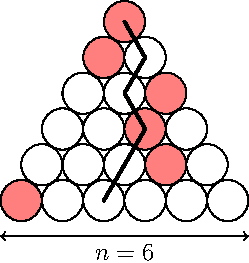
\includegraphics[scale=1]{IMO2023.pdf}
        \end{center}
  Như một hàm số theo $n$, tìm lớn nhất $k$ sao cho trong mỗi tam giác Nhật Bản có một con đường ninja chứa ít nhất $k$ các vòng tròn màu đỏ.
    \end{btvn}
    \subsection{\LARGE \textcolor{dk}{Lời giải}}

    \newpage
    \thispagestyle{plain}
    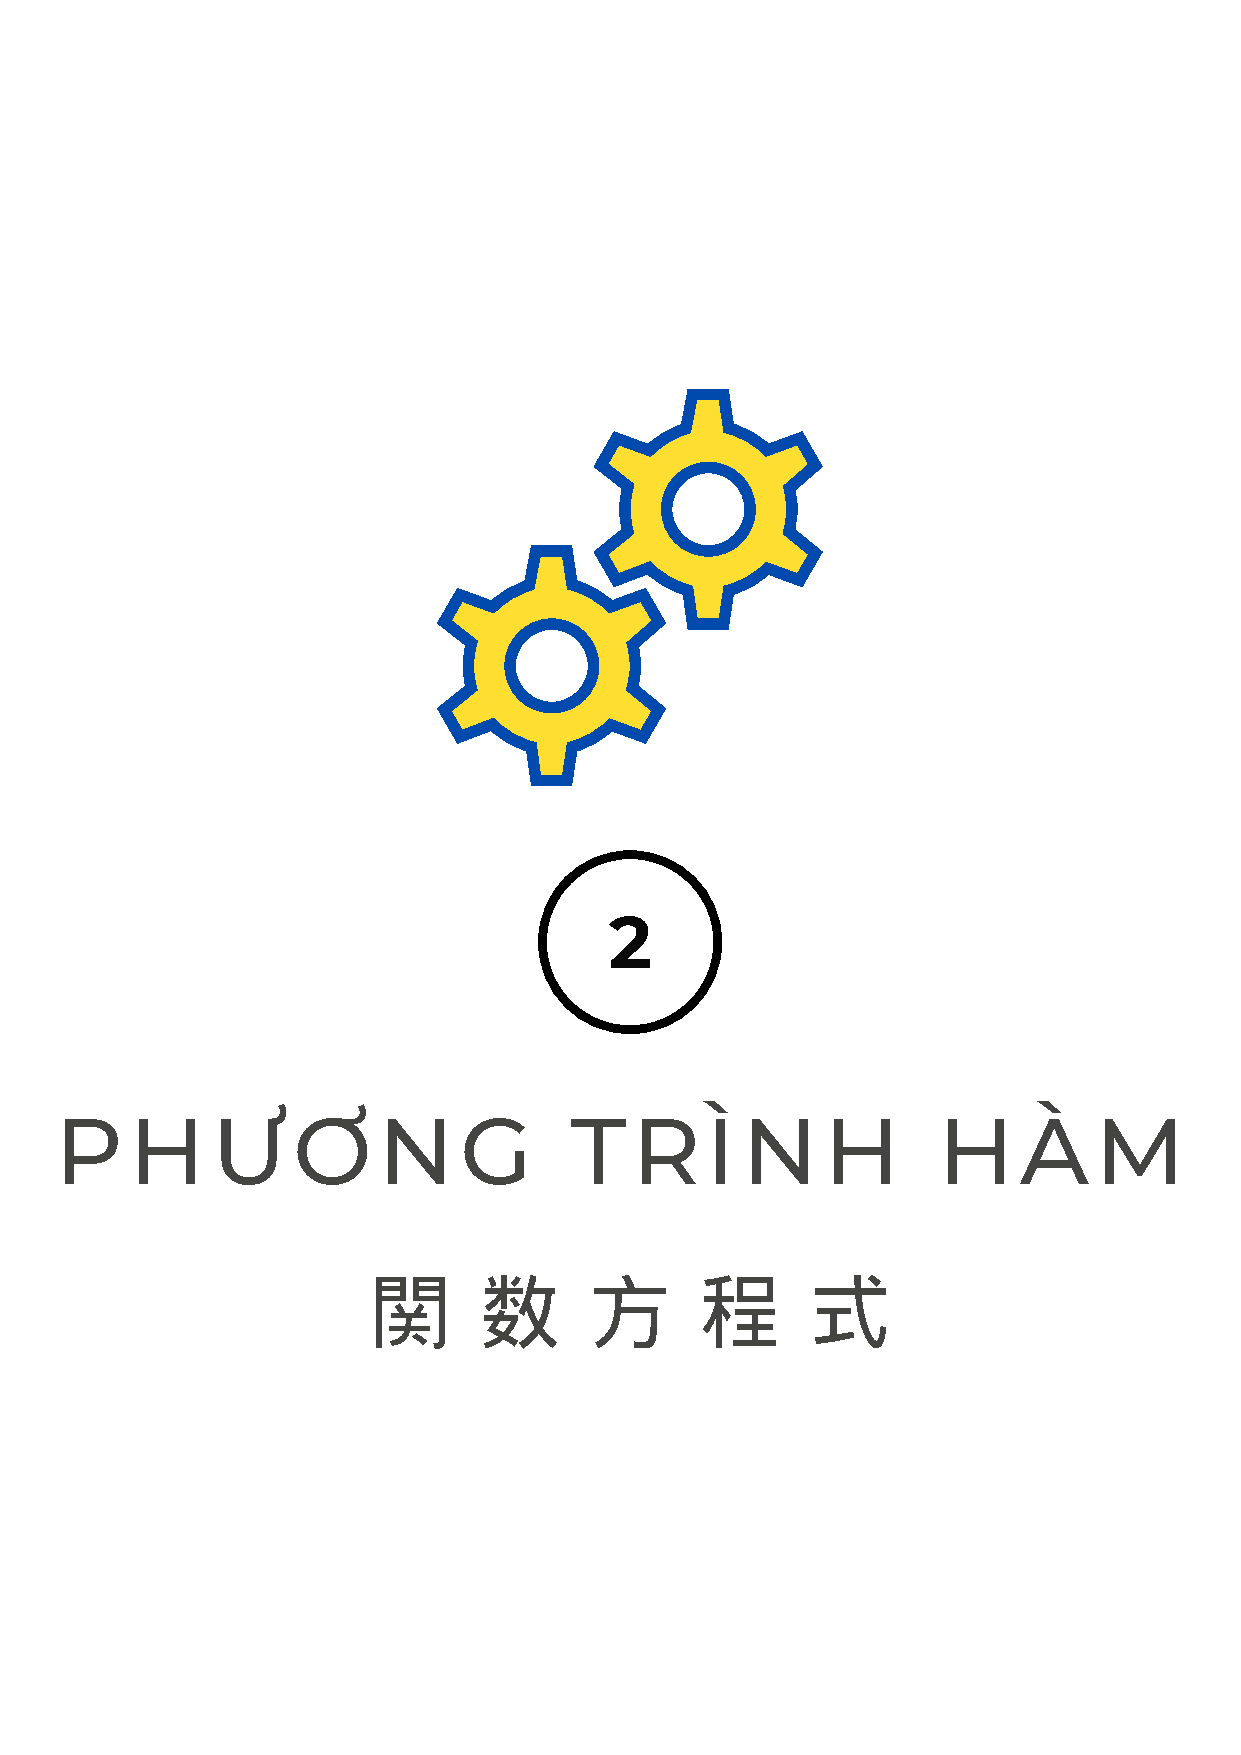
\includepdf[pages=1]{2.pdf}
    \section{\huge Phương trình hàm}
    \subsection{\LARGE \textcolor{dk}{Đề bài}}
    \item \begin{btvn}\vocab{(Bulgaria 1994).}
        Tìm tất cả các hàm số $f: \mathbb{R} \to \mathbb{R}$ thỏa mãn
        \[
            xf(x) -yf(y) =(x - y)f(x + y)
        \]
        với mọi số thực $x,y$.
    \end{btvn}
    \item \begin{btvn}\vocab{(VNTST 2004).}
        Tìm tất cả các giá trị thực của $a$ sao cho tồn tại duy nhất một hàm số $f: \mathbb{R} \to \mathbb{R}$ thỏa mãn
        \[
           f(x^2 + y+f(y)) = f(x)^2 + ay
        \]
        với mọi số thực $x,y$.
    \end{btvn}
    \item \begin{btvn}\vocab{(Kyrgyzstan MO 2012).}
        Tìm tất cả các hàm số $f: \mathbb{R} \to \mathbb{R}$ thỏa mãn
        \[
            f(f(x)^2 + f(y)) = xf(x) + y
        \]
    \end{btvn}
    với mọi số thực $x,y$.
    \item \begin{btvn}\vocab{(USAJMO 2015).}
        Tìm tất cả các hàm số $f: \mathbb{Q} \to \mathbb{Q}$ thỏa mãn
        \[
            f(x) + f(t) = f(y) + f(z)
        \]
        Với mọi số hữu tỉ $x < y < z < t$ tạo thành một cấp số cộng.
    \end{btvn}
    \item \begin{btvn}
        Tìm tất cả các hàm số $f: \mathbb{R} \to \mathbb{R}$ thỏa mãn
        \[
           f(x^2 + y) = f(x^{27} + 2y) + f(x^4)
        \]
        với mọi số thực $x,y$.
    \end{btvn}
    \item \begin{btvn}
        Tìm tất cả các hàm số $f: \mathbb{Z} \to \mathbb{Z}$ thỏa mãn
        \[
           f(f(x)) = x + 2
        \]
        với mọi số nguyên $x$.
    \end{btvn}
    \item \begin{btvn}
        Tìm tất cả các hàm số $f: \mathbb{R} \to \mathbb{R}$ thỏa mãn
        \[
           xf(x) + y^2 + f(xy) = f(x + y)^2 -f(x)f(y)
        \]
        với mọi số thực $x,y$.
    \end{btvn}
    \item \begin{btvn}\vocab{(USAMO 2002).}
        Tìm tất cả các hàm số $f: \mathbb{R} \to \mathbb{R}$ thỏa mãn
        \[
           f(x^2 - y^2) = xf(x) - yf(y)
        \]
        với mọi số thực $x,y$.
    \end{btvn}
    \item \begin{btvn}\vocab{(IMO 2017).}
        Tìm tất cả các hàm số $f: \mathbb{R} \to \mathbb{R}$ thỏa mãn
        \[
           f(f(x)f(y)) + f(x + y) = f(xy)
        \]
        với mọi số thực $x,y$.
    \end{btvn}
    \item \begin{btvn}\vocab{(USAMO 2018).}
        Tìm tất cả các hàm số $f: \mathbb{R}^+ \to \mathbb{R}^+$ thỏa mãn
        \[
           f\left(x + \frac{1}{y}\right) + f\left(y + \frac{1}{z}\right) + f\left(y + \frac{1}{z}\right)
        \]
        với mọi số thực dương $x,y,z$ thỏa mãn $xyz = 1$.
    \end{btvn}
    \item \begin{btvn}\vocab{(IMO 2008).}
        Tìm tất cả các hàm số $f: \mathbb{R} \to \mathbb{R}$ thỏa mãn
        \[
           \frac{f(w)^2 + f(x)^2}{f(y^2) + f(z^2)} = \frac{w^2 + x^2}{y^2 + z^2}
        \]
        với mọi số thực $x,y,z,w$ thỏa mãn $wx = yz$
    \end{btvn}
    \item \begin{btvn}\vocab{(IMO 2010).}
        Tìm tất cả các hàm số $f: \mathbb{R} \to \mathbb{R}$ thỏa mãn
        \[
            f(\lfloor x\rfloor y) = f(x)\lfloor f(y)\rfloor
        \]
        với mọi số thực $x,y$.
    \end{btvn}
    \item \begin{btvn}\vocab{(USAMO 2000).}
        Gọi một hàm số thực $f$ là siêu lồi nếu như 
        \[
            \frac{f(x) + f(y)}{2} \geq f\left(\frac{x +y}{2}\right) + |x - y|
        \]
        với mọi số thực $x,y$. Chứng minh rằng không bao tồn tại hàm $f$ siêu lồi.
    \end{btvn}
    \item \begin{btvn}\vocab{(IMOSL 2015).}
        Tìm tất cả các hàm số $f: \mathbb{Z}^+ \to \mathbb{Z}^+$ thỏa mãn
        \[
           f(m - f(n))  = f(f(m)) - f(n) -1
        \]
        với mọi số nguyên dương $x,y$.
    \end{btvn}
    \item \begin{btvn}\vocab{(ELMO 2014).}
        Tìm tất cả bộ ba $(f,g,h)$ hàm đơn ánh thỏa mãn 
        \[
           \begin{aligned}
            &f(x + f(y)) = g(x) + h(y)\\
            &g(x + g(y)) = h(x) + f(y) \\
            &h(x + h(y)) = f(x) + g(y)
           \end{aligned}
        \]
        với mọi số thực $x,y$.
    \end{btvn}
    \item \begin{btvn}\vocab{(IMOSL 2016).}
        Tìm tất cả các hàm số $f: \mathbb{R}^+ \to \mathbb{R}^+$ thỏa mãn
        \[
           xf(x^2)f(f(y)) + f(yf(x)) = f(xy)\left(f(f(x^2)) + f(f(y^2))\right)
        \]
        với mọi số thực dương $x,y$.
    \end{btvn}
    \item \begin{btvn}\vocab{(ELMOSL 2013).}
        Tìm tất cả các hàm số $f: \mathbb{R} \to \mathbb{R}$ thỏa mãn
        \[
           f(x) + f(y) = f(x + y) \text{ và }f(x^{2013}) = f(x)^{2013}
        \]
        với mọi số thực $x,y$.
    \end{btvn}
    \item \begin{btvn}\vocab{(TSTST 2013).}
        Tìm tất cả các hàm số $f: \mathbb{Z}^+ \to \mathbb{Z}^+$ thỏa mãn
        \[
           f^{abc - a}(abc) + f^{abc - b}(abc) + f^{abc - c}(abc) = a + b + c
        \]
        với mọi số nguyên dương $a,b,c$.
    \end{btvn}
    \item \begin{btvn}\vocab{(Gabriel Dospinescu).}
        Tìm tất cả các hàm số $f: \mathbb{Z}_{\geq 0} \to \mathbb{R}$ thỏa mãn
        \[
           f(x + y) + f(1) + f(xy) = f(x) + f(y) + f(1 + xy)
        \]
        với mọi số nguyên không âm $x,y$.
    \end{btvn}
    \item \begin{btvn}\vocab{(IMOSL 2004).}
        Tìm tất cả các hàm số $f: \mathbb{R} \to \mathbb{R}$ thỏa mãn
        \[
           f(x^2 + y^2 +2f(xy)) = \left(f(x + y)\right)^2
        \]
        với mọi số thực $x,y$.
    \end{btvn}
    \item \begin{btvn}\vocab{(HMMT 11/2015).}
        Xét hàm số $f: \mathbb{Z} \to \mathbb{Z}$ thỏa mãn
        \[
           f(f(x) + 2x + 20) = 15
        \]
        Một số nguyên $n$ được gọi là \textit{bất định} nếu như $f(n)$ có thể nhận được mọi giá trị. Những giá trị nguyên nào là \textit{bất định}?
    \end{btvn}
    \item \begin{btvn}\vocab{(IMO 2012).}
        Tìm tất cả các hàm số $f: \mathbb{Z} \to \mathbb{Z}$ thỏa mãn
        \[
          f(a)^2 + f(b)^2 + f(c)^2 = 2f(a)f(b) + 2f(b)f(c) + 2f(c)f(a)
        \]
        với mọi số nguyên $a,b,c$ thỏa mãn $a + b + c = 0$.
    \end{btvn}
    \item \begin{btvn}\vocab{(USA TST 2015).}
        Cho hàm số $f: \mathbb{Q} \to \mathbb{Q}$ sao cho với mọi $x,y \in \mathbb{Q}$ thì $f(x + y) - f(x) -f(y)$ là một số nguyên. Tìm giá trị của $c$ sao cho $f(x) - cx$ là số nguyên với mọi giá trị $x$ hữu tỉ.
    \end{btvn}
    \item \begin{btvn}\vocab{(IMOSL 2001).}
        Tìm tất cả các hàm số $f: \mathbb{R} \to \mathbb{R}$ thỏa mãn
        \[
            f(xy)(f(x) - f(y)) =(x-y)f(x)f(y)
        \]
        với mọi số thực $x,y$.
    \end{btvn}
    \item \begin{btvn}\vocab{(ELMOSL 2013).}
        Một hàm $f: \mathbb{Z}^+ \to \mathbb{Z}^+$ được gọi là \textit{bão hòa} nếu như
        \[
            f^{f^{f(n)}(n)}(n) = n
        \]
        với mọi số nguyên dương $n$. Tìm tất cả giá trị nguyên dương $m$ sao cho mọi hàm $f$ \textit{bão hòa} đều thỏa mãn: $f^{2014}(m) = m $
    \end{btvn}
    \item \begin{btvn}\vocab{(EGMO 2014).}
        Tìm tất cả các hàm số $f: \mathbb{R} \to \mathbb{R}$ thỏa mãn
        \[
           f(y^2 + 2xf(y) + f(x)^2) = (y + f(x))(x + f(y))
        \]
        với mọi số thực $x,y$.
    \end{btvn}
    \item \begin{btvn}\vocab{(IMO 2015).}
        Tìm tất cả các hàm số $f: \mathbb{R} \to \mathbb{R}$ thỏa mãn
        \[
           f(x + f(x + y)) + f(xy) = x + f(x + y) + yf(x)
        \]
        với mọi số thực $x,y$.
    \end{btvn}
    \item \begin{btvn}\vocab{(IMO 1998).}
        Tìm tất cả các hàm số $f: \mathbb{Z}^+ \to \mathbb{Z}^+$ thỏa mãn
        \[
           f(n^2f(m)) = mf(n)^2
        \]
        với mọi nguyên dương $m,n$.
    \end{btvn}
    \item \begin{btvn}\vocab{(VNTST 2022).}
         Cho số thực $\alpha$ và xét hàm số $\varphi(x)=x^2 e^{\alpha x}$ với mọi $x \in \mathbb{R}$. Tìm tất cả hàm số $f: \mathbb{R} \rightarrow \mathbb{R}$ thỏa mãn
            $$
            f(\varphi(x)+f(y))=y+\varphi(f(x))
            $$
            với mọi số thực $x, y$.
    \end{btvn}
    \item \begin{btvn}\vocab{(District MO 2022).}
        Tìm tất cả hàm số $f: \mathbb{R} \rightarrow \mathbb{R}$ thỏa mãn
        $$
        f(f(y-x)-x f(y))+f(x)=y(1-f(x))
        $$
        với mọi số thực $x, y$.
    \end{btvn}
    \item \begin{btvn}\vocab{(Iran MO 2022).}
        Tìm tất cả hàm số $f: \mathbb{R} \rightarrow \mathbb{R}$ thỏa mãn
        $$
        f(x f(y)+f(x)+y)=x y+f(x)+f(y)
        $$
        với mọi số thực $x, y$.
    \end{btvn}
    \item \begin{btvn}\vocab{(Kosovo MO 2022).}
        Tìm tất cả hàm số $f: \mathbb{R} \rightarrow \mathbb{R}$ thỏa mãn
        $$
        f(f(x-y)-y f(x))=x f(y)
        $$
        với mọi số thực $x, y$.
    \end{btvn}
    \item \begin{btvn}\vocab{(Kosovo TST 2022).}
        Tìm tất cả hàm số $f: \mathbb{R} \rightarrow \mathbb{R}$ thỏa mãn
        $$
        f\left(x^2\right)+2 f(x y)=x f(x+y)+y f(x)
        $$
        với mọi số thực $x, y$.
    \end{btvn}
    \item \begin{btvn}\vocab{(Malaysia TST 2022).}
        Tìm tất cả hàm số $f: \mathbb{R} \rightarrow \mathbb{R}$ thỏa mãn
        $$
        f(x f(x)+2 y)=f(x)^2+x+2 f(y)
        $$
        với mọi số thực $x, y$.
    \end{btvn}
    \item \begin{btvn}\vocab{(Malaysia TST 2022).}
        Tìm tất cả hàm số $f: \mathbb{R} \rightarrow \mathbb{R}$ thỏa mãn
        $$
        f\left(x^2+f(x+y)\right)=y+x f(x+1)
        $$
        với mọi số thực $x, y$.
    \end{btvn}
    \item \begin{btvn}\vocab{(MEMO 2022).}
        Tìm tất cả hàm số $f: \mathbb{R} \rightarrow \mathbb{R}$ thỏa mãn
        $$
        f(x + f(x + y)) = x + f(f(x) + y)
        $$
        với mọi số thực $x, y$.
    \end{btvn}
    \item \begin{btvn}\vocab{(DAMO 2022).}
        Tìm tất cả hàm số $f: \mathbb{R} \rightarrow \mathbb{R}$ thỏa mãn
        $$
            f(2xy +f(x)) = xf(y) + f(yf(x) + x)
        $$
        với mọi số thực $x, y$.
    \end{btvn}
    \item \begin{btvn}\vocab{(Nordic 2022).}
        Tìm tất cả hàm số $f: \mathbb{R} \rightarrow \mathbb{R}$ thỏa mãn đồng thời
        \begin{enumerate}
            \item $f(f(x) f(1-x))=f(x) \quad \forall x \in \mathbb{R}$.
            \item $f(f(x))=1-f(x) \quad \forall x \in \mathbb{R}$.
        \end{enumerate}
    \end{btvn}
    \item \begin{btvn}\vocab{(Romania EGMO TST 2022).}
        Tìm tất cả hàm số $f: \mathbb{R} \rightarrow \mathbb{R}$ thỏa mãn
            $$
            f(f(x)+y)=f\left(x^2-y\right)+4 y f(x)
            $$
            với mọi số thực $x, y$.
    \end{btvn}
    \item \begin{btvn}\vocab{(HMMT 2022).}
        Tìm tất cả hàm số $f: \mathbb{R} \backslash\{0\} \rightarrow \mathbb{R}$ thỏa mãn
        $$
        f(x)^2-f(y) f(z)=x(x+y+z)(f(x)+f(y)+f(z))
        $$
    \end{btvn}
    \item \begin{btvn}\vocab{(China TST 2022).}
        Tìm tất cả hàm số $f: \mathbb{R} \rightarrow \mathbb{R}$ thỏa mãn
        $$
        \{f(x f(y)+1), f(y f(x)-1)\}=\{x f(f(y))+1, y f(f(x))-1\}
        $$
        với mọi $x, y \in \mathbb{R}$, trong đó $\{a, b\}=\{c, d\} \Longleftrightarrow\left[\begin{array}{l}a=c, b=d \\ a=d, b=c\end{array}\right.$.
    \end{btvn}
    \item \begin{btvn}\vocab{(VMO 2022).}
        Tìm tất cả hàm số $f: \mathbb{R}^{+} \rightarrow \mathbb{R}^{+}$thỏa mãn
        $$
        f\left(\frac{f(x)}{x}+y\right)=1+f(y)
        $$
        với mọi số thực dương $x, y$.
    \end{btvn}
    \item \begin{btvn}\vocab{(Balkan 2022).}
        Tìm tất cả hàm số $f: \mathbb{R}^{+} \rightarrow \mathbb{R}^{+}$thỏa mãn
        $$
        f\left(y f(x)^3+x\right)=x^3 f(y)+f(x)
        $$
        với mọi số thực dương $x, y$.
    \end{btvn}
    \item \begin{btvn}\vocab{(APMO 2022).}
        Tìm tất cả hàm số $f, g: \mathbb{R}^{+} \rightarrow \mathbb{R}^{+}$thỏa mãn
        \begin{enumerate}
            \item $(f(x)+y-1)(g(y)+x-1)=(x+y)^2 \quad \forall x, y>0$
            \item $(-f(x)+y)(g(y)+x)=(x+y+1)(y-x-1) \quad \forall x, y>0$.
        \end{enumerate}
    \end{btvn}
    \item \begin{btvn}\vocab{(Iran TST 2022).}
        Tìm tất cả hàm số $f: \mathbb{R}^{+} \rightarrow \mathbb{R}^{+}$thỏa mãn
        $$
        f(x+f(y)+f(f(z)))=z+f(y+f(x))
        $$
        với mọi số thực dương $x, y, z$.
    \end{btvn}
    \item \begin{btvn}\vocab{(Czech-Polish-Slovak Match 2022).}
         Tìm tất cả hàm số $f: \mathbb{R}^{+} \rightarrow \mathbb{R}^{+}$thỏa mãn
        $$
        f\left(f(x)+\frac{y+1}{f(y)}\right)=\frac{1}{f(y)}+x+1
        $$
        với mọi số thực dương $x, y$.
    \end{btvn}
    \item \begin{btvn}\vocab{(Switzerland TST 2022).}
         Tìm tất cả hàm số $f: \mathbb{R}^{+} \rightarrow \mathbb{R}^{+}$thỏa mãn
        $$
        x+f(y f(x)+1)=x f(x+y)+y f(y f(x))
        $$
        với mọi số thực dương $x, y$.
    \end{btvn}
    \item \begin{btvn}\vocab{(Taiwan TST 2022, Round 2).}
        Tìm tất cả hàm số $f: \mathbb{R}^{+} \rightarrow \mathbb{R}^{+}$thỏa mãn
        $$
        f\left(x+y^2 f(y)\right)=f(1+y f(x)) f(x)
        $$
        với mọi số thực dương $x, y$.
   \end{btvn}
   \item \begin{btvn}\vocab{(USAMO 2022).}
     Tìm tất cả hàm số $f: \mathbb{R}^{+} \rightarrow \mathbb{R}^{+}$thỏa mãn
    $$
    f(x)=f(f(f(x))+y)+f(x f(y)) f(x+y)
    $$
\end{btvn}
    \item \begin{btvn}\vocab{(Japan MO Final 2016). }
        Tìm tất cả các hàm số $f: \mathbb{R}\rightarrow \mathbb{R}$ thỏa mãn
        \[f(yf(x)-x)=f(x)f(y)+2x, \forall x,y \in \mathbb{R}\]
    \end{btvn}

    \item \begin{btvn}\vocab{(Japan MO Final 2018).}
        Cho tập hợp $S=\{1,2,\ldots ,999\}$. Xét hàm số $f: S\to S$, sao cho với mọi $n\in S$,
        $$f^{n+f(n)+1}(n)=f^{nf(n)}(n)=n.$$
        Chứng minh rằng tồn tại $a\in S$, sao cho $f(a)=a$. Ở đây có $f^k(n) = \underbrace{f(f(\ldots f}_{k}(n)\ldots))$.
    \end{btvn}
    \item \begin{btvn}\vocab{(British MO 2022).}
        Tìm tất cả hàm số $f: \mathbb{Z}^{+} \rightarrow \mathbb{Z}^{+}$thỏa mãn
        $$
        \left.2 b f\left(f\left(a^2\right)+a\right)\right)=f(a+1) f(2 a b)
        $$
        với mọi số nguyên dương $a, b$.
    \end{btvn}
    \item \begin{btvn}\vocab{(Francophone MO 2022).}
         Tìm tất cả hàm số $f: \mathbb{Z} \rightarrow \mathbb{Z}$ thỏa mãn
            $$
            f(m+n)+f(m) f(n)=n^2(f(m)+1)+m^2(f(n)+1)+m n(2-m n)
            $$
            với mọi số nguyên $m, n$.
    \end{btvn}
    \item \begin{btvn}\vocab{(Taiwan TST 2022, Round 1 ).}
         Tìm tất cả hàm số $f: \mathbb{Z} \rightarrow \mathbb{Z}$ thỏa mãn
        $$
        f\left(\left\lfloor\frac{f(x)+f(y)}{2}\right\rfloor\right)+f(x)=f(f(y))+\left\lfloor\frac{f(x)+f(y)}{2}\right\rfloor
        $$
        với mọi số nguyên $x, y$, trong đó ký hiệu $\lfloor x\rfloor$ chỉ số nguyên lớn nhất không vượt quá $x$.
    \end{btvn}

    \item \begin{btvn}\vocab{(Japan MO Final 2019).}
        Tìm tất cả các hàm số $f: \mathbb{R}^+\rightarrow \mathbb{R}^+$ thỏa mãn
        \[f\left(\frac{f(y)}{f(x)}+1\right)=f\left(x+\frac{y}{x}+1\right)-f(x)\]
    \end{btvn}

    \item \begin{btvn}\vocab{(Japan MO Final 2020).}
        Tìm tất cả các hàm số $f: \mathbb{Z}^+\rightarrow \mathbb{Z}^+$ thỏa mãn
        \[m^{2}+f(n)^{2}+(m-f(n))^{2}\geq f(m)^{2}+n^{2},\forall m,n \in \mathbb{Z}^+\]
    \end{btvn}
    \item \begin{btvn}\vocab{(USA TSTST 2022).}
        Tìm tất cả hàm số $f: \mathbb{Z}^{+} \rightarrow \mathbb{Z}$ thỏa mãn
        $$
        \left\lfloor\frac{f(m n)}{n}\right\rfloor=f(m)
        $$
        với mọi số nguyên dương $m, n$.
    \end{btvn}
    \item \begin{btvn}\vocab{(MEMO 2022). }
        Tìm tất cả hàm số $f: \mathbb{Z}^{+} \rightarrow \mathbb{Z}^{+}$sao cho $f(1) \leq f(2) \leq f(3) \leq$ $f(4) \leq \ldots$ và
        $$
        f(n)+n+1, \quad f(f(n))-f(n)
        $$
        đều là số chính phương với mọi số nguyên dương $n$.
    \end{btvn}
    \item \begin{btvn}\vocab{(IMO 2022).}
         Tìm tất cả hàm số $f: \mathbb{R}^{+} \rightarrow \mathbb{R}^{+}$sao cho với mỗi số thực dương $x$, tồn tại duy nhất số thực dương $y$ thỏa mãn
            $$
            x f(y)+y f(x) \leq 2 .
            $$
    \end{btvn}
    \item \begin{btvn}\vocab{(Japan MO Final 2021).}
        Tìm tất cả các hàm số $f: \mathbb{Z}^+\rightarrow \mathbb{Z}^+$ thỏa mãn hai điều kiện sau
        \[
            n \mid m \text{ và }f(n) \mid f(m) - n
        \]
    \end{btvn}
    \item \begin{btvn}\vocab{(AUS 2022).}
         Tìm tất cả hàm số $f:[1 ;+\infty) \rightarrow[0 ;+\infty)$ thỏa mãn
        $$
        f(2 f(x)+y) \geq f\left(x^3\right)+f\left(y^2 f(x)+x^2+x y\right)
        $$
        với mọi số thực $x, y \geq 1$.
    \end{btvn}
    \item \begin{btvn}\vocab{Abel Competition Final 2021-2022).}
         Tìm tất cả hàm số $f: \mathbb{R}^{+} \rightarrow \mathbb{R}^{+}$thỏa mãn
        $$
        f\left(\frac{1}{x}\right) \geq 1-\frac{\sqrt{f(x) f\left(\frac{1}{x}\right)}}{x} \geq x^2 f(x)
        $$
        với mọi số thực dương $x$.
    \end{btvn}
    \item \begin{btvn}\vocab{(Indonesia TST 2022). }
        Tìm tất cả hàm số $f: \mathbb{R} \rightarrow \mathbb{R}$ thỏa mãn
        $$
        f\left(x^2\right)-f\left(y^2\right) \leq(f(x)+y)(x-f(y))
        $$
        với mọi số thực $x, y$.
    \end{btvn}
    \item \begin{btvn}\vocab{(Philippine MO 2022).}
         Tìm tất cả hàm số $f: \mathbb{R} \rightarrow \mathbb{R}$ thỏa mãn
            $$
            f(a-b) f(c-d)+f(a-d) f(b-c) \leq(a-c) f(b-d)
            $$
            với mọi số thực $a, b, c$ và $d$.
    \end{btvn}
    \item \begin{btvn}\vocab{(Japan MO Final 2022).}
        Tìm tất cả các hàm số $f: \mathbb{Z}^+\rightarrow \mathbb{Z}^+$ thỏa mãn
        \[f^{f(n)}(m)+mn=f(m)f(n)\]
    \end{btvn}
    \item \begin{btvn}\vocab{(Hà Tĩnh TST 2023).}
        Tìm tất cả các hàm số $f: \bb{R} \to \bb{R}$ thỏa mãn 
        \[
            f(xf(x + y)) = f(yf(x)) + x^2
        \]
        với mọi số thực $x,y$.
    \end{btvn}
    \item \begin{btvn}\vocab{(Japan MO Final 2024).}
        Tìm tất cả các hàm số $f: \mathbb{Z}^+\rightarrow \mathbb{Z}^+$ thỏa mãn
        \[\text{lcm}(m, f(m+f(n)))=\text{lcm}(f(m), f(m)+n), \forall m,n \in \mathbb{Z}^+\]
    \end{btvn}
    \item \begin{btvn}\vocab{(VMO 2003).}
        Cho $f: \mathbb{R}\to\mathbb{R}$ là một hàm sao cho $f( \cot x ) = \cos 2x+\sin 2x$ với mọi $0 < x < \pi$. Cho $g(x) = f(x) f(1-x)$ với mọi$-1 \leq x \leq 1$. Tìm các giá trị lớn nhất và nhỏ nhất của $g$ trên khoảng thời gian đóng $[-1, 1].$
    \end{btvn}
    \item \begin{btvn}\vocab{(VMO 2012).}Tìm tất cả hàm số $f:\mathbb{R} \to \mathbb{R}$ thỏa mãn:
    \begin{enumerate}
        \item $f$ là hàm toàn ánh
        \item $f$ tăng nghiêm ngặt
        \item $f(f(x))=f(x)+12x.$
    \end{enumerate}      
    \end{btvn}
    \begin{btvn}\vocab{(VMO 2013).}Tìm tất cả các hàm số $f:\mathbb{R}\rightarrow\mathbb{R}$ thỏa mãn $f(0)=0,f(1)=2013$ và 
        \[(x-y)(f(f(x)^2)-f(f(y)^2))=(f(x)-f(y))(f(x)^2-f(y)^2)\]
        với mọi số thực $x,y$.
    \end{btvn}
    \item \begin{btvn}\vocab{(VMO 2016).} Tìm tất cả hàm số $f:\mathbb{R} \to \mathbb{R}$ thỏa mãn:
        \begin{enumerate}
            \item $f(1) = 2016$
            \item $f(x+y+f(y))=f(x)+ay\quad\forall x,y\in\mathbb{R}$
        \end{enumerate}      
    \end{btvn}
    \item \begin{btvn}\vocab{(VMO 2017).} Tìm tất cả các hàm số $f:\mathbb{R} \to \mathbb{R}$ thỏa mãn:
        $$f(xf(y)-f(x))=2f(x)+xy$$
    với mọi số thực $x,y$.
    \end{btvn}
    \item \begin{btvn}\vocab{(VMO 2021).} Tìm tất cả các hàm số $f:\mathbb{R} \to \mathbb{R}$ thỏa mãn:
        \[f(x)f(y)=f(xy-1)+yf(x)+xf(y)\]
    với mọi số thực $x,y$.
    \end{btvn}
    \item \begin{btvn}\vocab{(VMO 2023).} Tìm tất cả các cặp hàm số $f,g:\mathbb{R} \to \mathbb{R}$ thỏa mãn $f(0) = 2022$ và
        \[f (x+g(y)) =xf(y)+(2023-y)f(x)+g(x)\]
    với mọi số thực $x,y$.
    \end{btvn}
    \item \begin{btvn}\vocab{(KMF 2022).}
        Cho hàm số $g \colon \mathbb{R} \to \mathbb{R}$ sao cho miền giá trị của nó là một tập hữu hạn. Tìm tất cả các hàm $f \colon \mathbb{R} \to \mathbb{R}$ thỏa mãn
        $$2f(x+g(y))=f(2g(x)+y)+f(x+3g(y)), \forall x,y \in \mathbb{R}$$
    \end{btvn}
    \item \begin{btvn}\vocab{(Balkan MO 2021).} Tìm tất cả các hàm số $f:\mathbb{R}^+ \to \mathbb{R}^+$ thỏa mãn:
        \[f(x+f(x)+f(y))=2f(x)+y\]
    với mọi số thực dương $x,y$.
    \end{btvn}
    \item \begin{btvn}\vocab{(Balkan MO 2022).} Tìm tất cả các hàm số $f:\mathbb{R}^+ \to \mathbb{R}^+$ thỏa mãn:
        \[f(y(f(x))^3 + x) = x^3f(y) + f(x)\]
    với mọi số thực dương $x,y$.
    \end{btvn}
    \item \begin{btvn}\vocab{(KMF 2022).}
    Tìm tất cả các hàm số $f,g: \mathbb{R} \to \mathbb{R}$ thỏa mãn:
    $$f(x^2-g(y))=g(x)^2-y, \forall x,y \in \mathbb{R}$$
    \end{btvn}
    \item \begin{btvn}\vocab{(Balkan MO 2023).} Tìm tất cả các hàm số $f:\mathbb{R} \to \mathbb{R}$ thỏa mãn:
        \[xf(x+f(y))=(y-x)f(f(x))\]
    với mọi số thực $x,y$.
    \end{btvn}
    \item \begin{btvn}\vocab{(Iran MO 2023).}
        Tìm tất cả các hàm số $f: \mathbb{C} \to \mathbb{C}$ thỏa mãn:
        \[
            f(f(x) + yf(y)) = x + |y|^2, \forall x,y \in \mathbb{C}
        \]
        Chú ý ở đây nếu $y = a + bi$ thì $|y| = \sqrt{a^2 + b^2}$, $a,b \in R$.
    \end{btvn}
    \item \begin{btvn}\vocab{(Balkan MO 2024).}
        Tìm tất cả các hàm số $f : \mathbb{R}^+ \to \mathbb{R}^+$ và đa thức $P(x)$ với hệ số thực không âm thỏa mãn $P(0) = 0$ và \[f(f(x) + P(y)) = f(x - y) + 2y\] với mọi số thực dương $x > y > 0$.
    \end{btvn}
    \item \begin{btvn}\vocab{(VNTST 2014).} Tìm tất cả các hàm số $f:\mathbb{Z}\to \mathbb{Z}$ thỏa mãn:
        \[ f(2m+f(m)+f(m)f(n))=nf(m)+m \]
    với mọi số nguyên $m,n$.
    \end{btvn}
    \item \begin{btvn}\vocab{(VNTST 2024).}Cho đa thức monic $P(x) \in \mathbb{R}[x]$ khác hằng. Tìm tất cả các hàm số liên tục $f: \mathbb{R} \to \mathbb{R}$ thỏa mãn
        $$f(f(P(x))+y+2023f(y))=P(x)+2024f(y),$$
        với mọi số thực $x,y$.
    \end{btvn}
    \item \begin{btvn}\vocab{(IMOSL 2010 A5).}
        Tìm tất cả các hàm số $f : \mathbb{Q}^+ \mapsto \mathbb{Q}^+$ thỏa mãn
        \[f\left( f(x)^2y \right) = x^3 f(xy)\]
        với mọi $x,y$ hữu tỉ.
    \end{btvn}
    \item \begin{btvn}\vocab{(IMOSL 2011 A3).}
        Tìm tất cả các cặp hàm số $f,g: \mathbb{R} \to \mathbb{R}$ thỏa mãn
        \[g(f(x+y)) = f(x) + (2x + y)g(y)\]
        với mọi số thực $x,y$.
    \end{btvn}
    \item \begin{btvn}\vocab{(IMOSL 2011 A4).}
        Tìm tất cả các cặp hàm số $f,g: \mathbb{Z}^+ \to \mathbb{Z}^+$ thỏa mãn
        \[f^{g(n)+1}(n) + g^{f(n)}(n) = f(n+1) - g(n+1) + 1\]
        với mọi nguyên dương $n$.
    \end{btvn}
    \item \begin{btvn}\vocab{(IMOSL 2011 A6).}
        Cho hàm số $f: \mathbb{R} \to \mathbb{R}$ thỏa mãn
        \[f(x + y) \leq yf(x) + f(f(x))\]
        với mọi số thực $x,y$. Chứng minh rằng $f(x) = 0$ với mọi $x \leq 0$.
    \end{btvn}
    \item \begin{btvn}\vocab{(IMOSL 2012 A5).}
        Tìm tất cả các hàm số $f : \mathbb{R} \mapsto \mathbb{R}$ thỏa mãn
        \[f(1+xy)-f(x+y)=f(x)f(y) \]
        với mọi số thực $x,y$.
    \end{btvn}
    \item \begin{btvn}\vocab{(IMOSL 2014 A4).}
        Tìm tất cả các hàm số $f : \mathbb{Z} \mapsto \mathbb{Z}$ thỏa mãn
        \[ n^2+4f(n)=f(f(n))^2 \]
        với mọi số nguyên $n$.
    \end{btvn}
    \item \begin{btvn}\vocab{(IMOSL 2014 A6).}
        Tìm tất cả các hàm số $f : \mathbb{Z} \mapsto \mathbb{Z}$ thỏa mãn
        \[f\big(f(m)+n\big)+f(m)=f(n)+f(3m)+2014\]
        với mọi số nguyên $m,n$.
    \end{btvn}
    \item \begin{btvn}\vocab{(IMOSL 2015 A2).}
        Tìm tất cả các hàm số $f : \mathbb{Z} \mapsto \mathbb{Z}$ thỏa mãn
        \[f(x-f(y))=f(f(x))-f(y)-1\]
        với mọi số nguyên $x,y$.
    \end{btvn}

    \item \begin{btvn}\vocab{(IMOSL 2015 A5).}
        Cho $2\mathbb{Z} + 1$ là tập các số nguyên lẻ. Tìm tất cả các hàm số $f : \mathbb{Z} \mapsto 2\mathbb{Z} + 1$ thỏa mãn
        \[ f(x + f(x) + y) + f(x - f(x) - y) = f(x+y) + f(x-y) \]
        với mọi số nguyên $x,y$.
    \end{btvn}
    \item \begin{btvn}\vocab{(IMOSL 2016 A4).}
        Tìm tất cả các hàm số $f : \mathbb{R}^+ \mapsto \mathbb{R}^+$ thỏa mãn
        $$xf(x^2)f(f(y)) + f(yf(x)) = f(xy) \left(f(f(x^2)) + f(f(y^2))\right).$$
        với mọi số thực dương $x,y$.
    \end{btvn}
    \item \begin{btvn}\vocab{(IMOSL 2016 A7).}
        Tìm tất cả các hàm số $f : \mathbb{R} \mapsto \mathbb{R}$ thỏa mãn $f(0)\neq 0$ và
        \[ f(x+y)^2 = 2f(x)f(y) + \max \left\{ f(x^2+y^2), f(x^2)+f(y^2) \right\}. \]
        với mọi số thực $x,y$.
    \end{btvn}
    \item \begin{btvn}\vocab{(IMOSL 2017 A6).}
        Tìm tất cả các hàm số $f : \mathbb{R} \mapsto \mathbb{R}$ thỏa mãn
        \[ f(f(x)f(y)) + f(x+y) = f(xy). \]
        với mọi số thực $x,y$.
    \end{btvn}

    \item \begin{btvn}\vocab{(IMOSL 2017 A8).}
        Một hàm số $f: \mathbb{R} \to \mathbb{R}$ có tính chất 

        Với mọi $x,y \in \mathbb{R}$ sao cho $(f(x)+y)(f(y)+x) > 0$ thì ta luôn có $f(x)+y = f(y)+x$

        Chứng minh rằng $f(x)+y \leq f(y)+x$ với $x > y$.
    \end{btvn}

    \item \begin{btvn}\vocab{(IMOSL 2018 A1).}
        Tìm tất cả các hàm số $f: \mathbb{Q}^+ \to \mathbb{Q}^+$ thỏa mãn
        $$f(x^2f(y)^2)=f(x)^2f(y)$$
        với mọi số hữu tỉ dương $x,y$.
    \end{btvn}

    \item \begin{btvn}\vocab{(IMOSL 2018 A5).}
        Tìm tất cả các hàm số $f : \mathbb{R}^+ \mapsto \mathbb{R}$ thỏa mãn
        $$\left(x+\frac{1}{x}\right)f(y)=f(xy)+f\left(\frac{y}{x}\right)$$
        với mọi số thực dương $x,y$.
    \end{btvn}
    \item \begin{btvn}\vocab{(IMOSL 2019 A1).}
        Tìm tất cả các hàm số $f: \mathbb{Z} \to \mathbb{Z}$ thỏa mãn
        $$f(2a)+2f(b)=f(f(a+b)).$$
        với mọi số nguyên $a,b$.
    \end{btvn}

    \item \begin{btvn}\vocab{(IMOSL 2020 A6).}
        Tìm tất cả các hàm số $f: \mathbb{Z} \to \mathbb{Z}$ thỏa mãn
        \[f^{a^{2} + b^{2}}(a+b) = af(a) +bf(b)\]
        với mọi số nguyên $a,b$.
    \end{btvn}

    \item \begin{btvn}\vocab{(IMOSL 2020 A8).}
        Tìm tất cả các hàm số $f : \mathbb{R} \mapsto \mathbb{R}$ thỏa mãn
        $$f(x+f(xy))+y=f(x)f(y)+1$$
        với mọi số thực $x,y$.
    \end{btvn}

    \item \begin{btvn}\vocab{(IMOSL 2021 A8).}
        Tìm tất cả các hàm số $f : \mathbb{R} \mapsto \mathbb{R}$ thỏa mãn
        $$(f(a)-f(b))(f(b)-f(c))(f(c)-f(a)) = f(ab^2+bc^2+ca^2) - f(a^2b+b^2c+c^2a)$$
        với mọi số thực $a,b,c$.
    \end{btvn}
    \item \begin{btvn}\vocab{(Đồng Tháp TST 2023).}
        Tìm tất cả các hàm số $f: \mathbb{R} \to \mathbb{R}$ thỏa mãn
        \[
            f(x + y) + f(x - y) - 2f(x)f(y + 1) = xy
        \]
        với mọi số thực $x,y$.
    \end{btvn}
    \item \begin{btvn}\vocab{(Bình Phước TST 2023).}
        Tìm tất cả các hàm số $f: \mathbb{R} \to \mathbb{R}$ thỏa mãn
        \[
            f(xf(x) + f(y)) = f(x)^2 + y
        \]
        với mọi số thực $x,y$.
    \end{btvn}
    \item \begin{btvn}\vocab{(An Giang TST 2023).}
        Tìm tất cả các hàm số $f: \mathbb{R} \to \mathbb{R}$ thỏa mãn
        \[
            f(x^2 + f(y)) = y + f(x)^2
        \]
        với mọi số thực $x,y$.
    \end{btvn}
    \item \begin{btvn}\vocab{(Thanh Hóa TST 2023).}
        Tìm tất cả các hàm số $f: \mathbb{R} \to \mathbb{R}$ thỏa mãn
        \[
            f(f(y) + x^2 + 1) + 2x = y + f(x + 1)^2
        \]
        với mọi số thực $x,y$.
    \end{btvn}
    \item \begin{btvn}\vocab{(TST Tiền Giang 2023).}
        Gọi $S$ là tập số thực hữu hạn lớn hơn $-1$. Tìm tất cả các hàm số $f: S \to S$ thỏa mãn:
        \begin{enumerate}
            \item $f(x + f(y) + xf(y)) = y + f(x) +yf(x), \forall x,y \in S$
            \item Hàm số $g(x) = \frac{f(x)}{x}$ tăng thực sự trên $(-1,0)$ và $(0, +\infty)$.
        \end{enumerate}
    \end{btvn}
    \item \begin{btvn}\vocab{(Trại hè Hùng Vương 2023).}
        Tìm tất cả các hàm số $f : \bb{R} \to \bb{R}$ thỏa mãn:
        \[
            xf(x + f(y)) = (y - x)f(f(x))
        \]
        với mọi số thực $x,y$.
    \end{btvn}
    \item \begin{btvn}\vocab{(Đồng Nai TST 2023).}
        Tìm tất cả các hàm số $f: \bb{Z} \to \bb{Z}$ thỏa mãn
        \[
            f(2a) + 2f(b) = f(2(a + b))
        \]
        với mọi số nguyên $a,b$.
    \end{btvn}
    \item \begin{btvn}\vocab{(PTNK 2023).}
        Tìm tất cả các hàm số $f: \bb{R} \to \bb{R}$ thỏa mãn $f(x + 1) =f(x) + 1$ và
        \[
            f(x^{2024} + x^{2023} + \dots + x + 1) = (f(x))^{2024} + (f(x))^{2023} + \dots + f(x) + 1
        \]
    \end{btvn}
    \item \begin{btvn}\vocab{(APMO 2023).}
        Cho số thực dương $c > 0$. Tìm tất cả các hàm số $f: \bb{R}^+ \to \bb{R}^+$ thỏa mãn
        \[
            f((c + 1)x +f(y)) = f(x + 2y) +2cx
        \]
        với mọi số thực dương $x,y$.
    \end{btvn}
    \subsection{\LARGE \textcolor{dk}{Lời giải}}
    \newpage
    \thispagestyle{plain}
    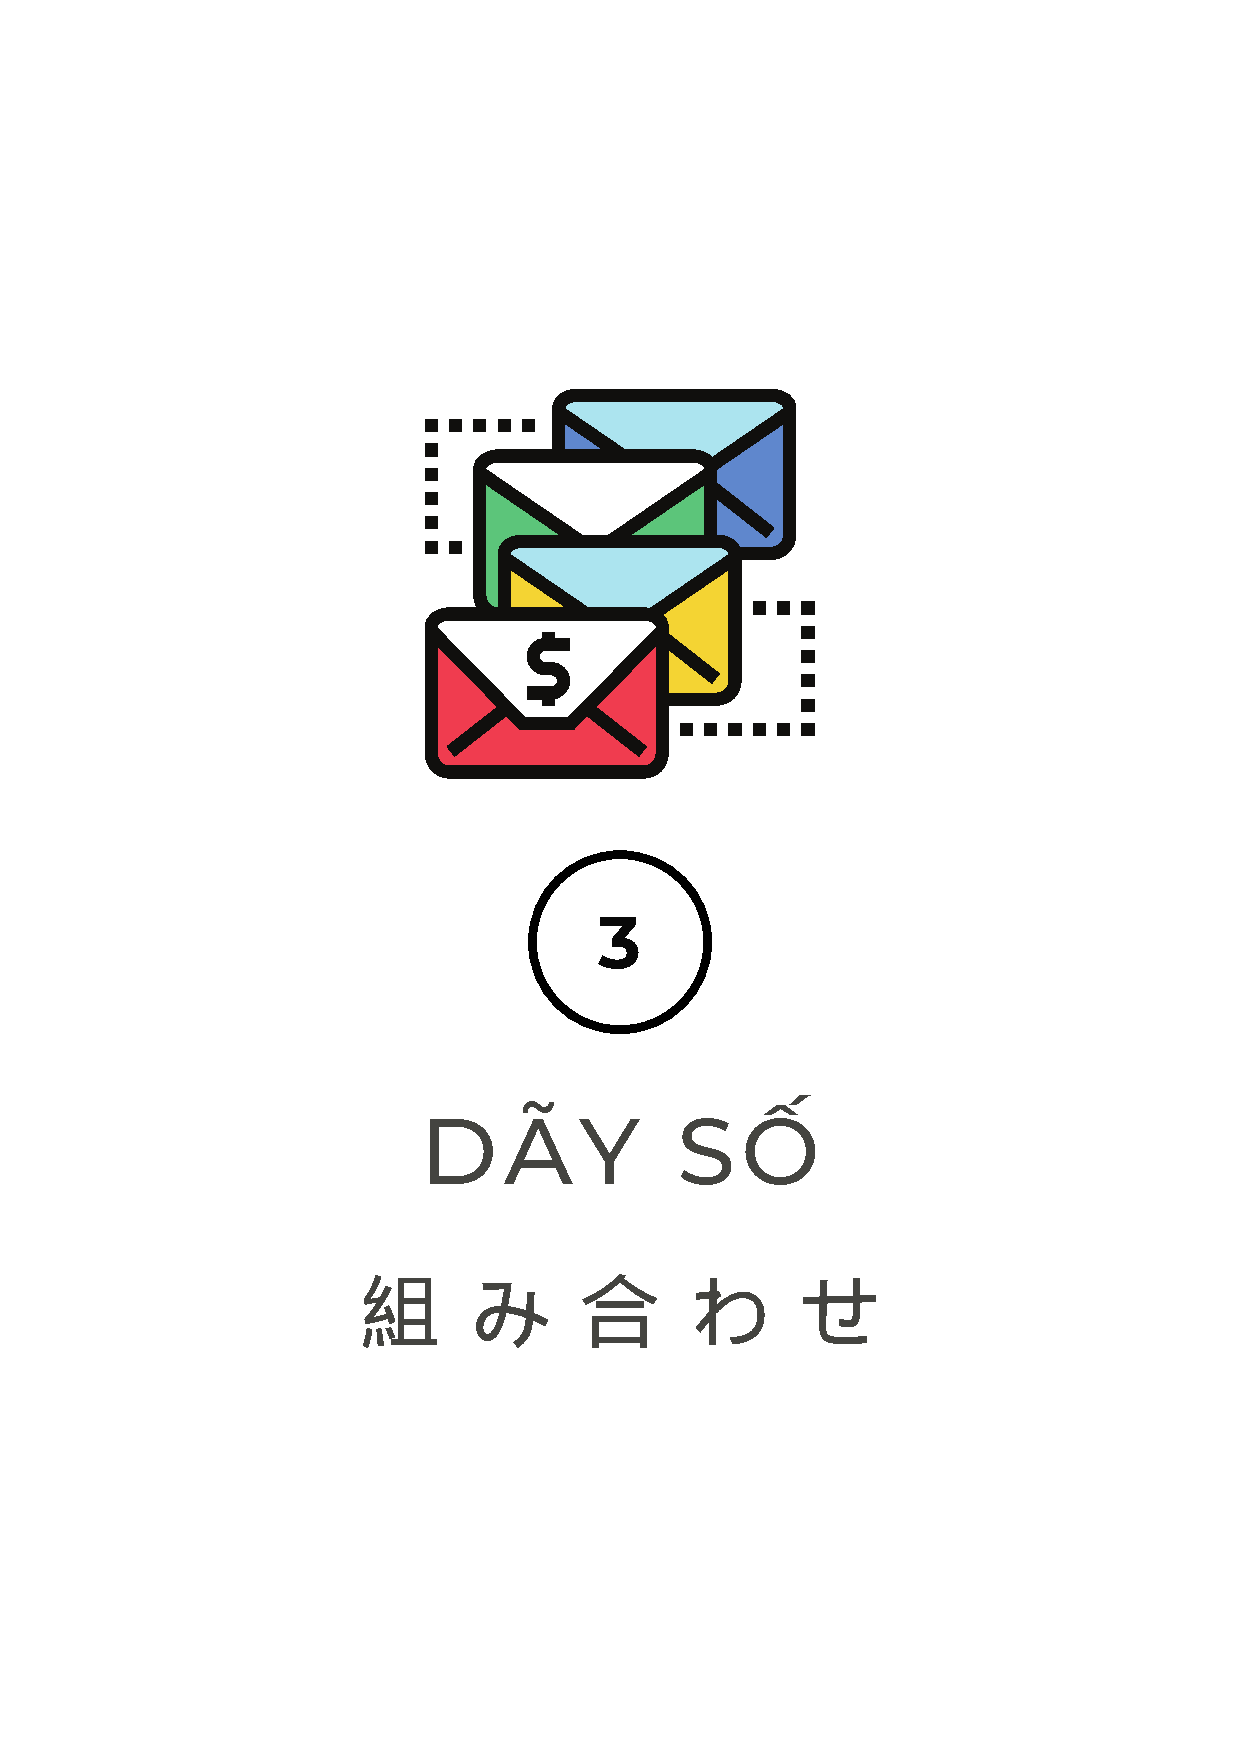
\includepdf[pages=1]{3.pdf}
    \section{\huge Dãy số}
    \subsection{\LARGE \textcolor{dk}{Đề bài}}
    \item \begin{btvn}\vocab{(Đồng Nai TST 2023).}
        Cho dãy số $(a_n)$ thỏa mãn $a_1 = 1$ và $$a_{n + 1} = \sqrt{2n + a_n^2 + \frac{1}{a_n}}, n \geq 1$$.
        \begin{enumerate}[label=(\alph*)]
            \item Chứng minh rằng $a_n \leq n$, với mọi số nguyên dương $n$.
            \item Tìm $\dlim$
        \end{enumerate}
    \end{btvn}
    \item \begin{btvn}\vocab{(Hà Tĩnh TST 2023).}
        Cho dãy số $(u_n)$ xác định bởi $u_1 = 1$ và $$u_{n + 1} = 1 + \frac{1}{u_n + 1}, n \geq 1$$
        \begin{enumerate}[label=(\alph*)]
            \item Chứng minh rằng dãy số $(u_n)$ có giới hạn hữu hạn và tìm giới hạn đó.
            \item Chứng minh rằng $\dsum_{i = 1}^n u_i^2 < 2n, n \geq 1$.
        \end{enumerate}
    \end{btvn}
    \item \begin{btvn}\vocab{(Hà Nội TST 2022).}
        Cho dãy $(x_n)$ được xác định bởi $x_1 = x_2 = 1$ và $x_{n + 2} = x_{n + 1}^2 - \frac{1}{3}x_n$ với $n \geq 1$. Chứng minh rằng $(x_n)$ có giới hạn hữu hạn và tìm giới hạn đó.
    \end{btvn}
    \item \begin{btvn}\vocab{(PTNK 2023).}
        Cho dãy $(u_n)$ thỏa mãn $u_1 = 1$ và $u_{n + 1} = u_n + \frac{\ln n}{u_n}, n \geq 1$.
        \begin{enumerate}[label=(\alph*)]
            \item Chứng minh rằng $u_{2023} > \sqrt{2023 \ln 2023}$
            \item Tìm $\dlim\frac{u_n  \ln n}{n}$.
        \end{enumerate}
    \end{btvn}
    \item \begin{btvn}\vocab{(Trại hè Hùng Vương 2023).}
        Cho dãy số $(u_n)$ được xác định bởi $u_1 = 3$ và $$u_{n + 1} = u_n^2 + u_n - 4, n \geq 1$$ Tìm $\dlim\frac{(u_1 + 1)(u_2 + 3)\dots(u_n + 3)}{u_{n + 1} +3}$.
    \end{btvn}
    \item \begin{btvn}\vocab{(PTNK 2022).}
        Cho dãy số $(u_n)$ được xác định bởi $u_1 = 1$ và $u_{n + 1} = \sqrt{2 + u_n}, n \geq 1$. Tính
        \[
            \lim_{n \to + \infty} \frac{1}{\ln n}\left(\frac{u_1}{1} + \frac{u_2}{2} + \dots + \frac{u_n}{n}\right)
        \]
    \end{btvn}
    \item \begin{btvn}\vocab{(Bình Phước TST 2023).}
        Cho đãy số $\left(a_n\right)$ xác định bởi: \[\left\{\begin{array}{l}a_1=\frac{2024}{2023} \\ a_{n+1}=a_n+2 \sqrt{a_n}+\frac{n^2}{a_n}, \forall n \geq 1 .\end{array}\right.\]
        \begin{enumerate}[label=(\alph*)]
            \item Chứng minh rằng dãy số $\left(b_n\right)$ xác định bởi $b_n=\dsum_{i=1}^n \frac{1}{a_i}$ có giới hạn hữu hạn.
            \item Xét dãy số $\left(c_n\right)$ xác định bởi $c_n=\left[\dsum_{i=1}^n \frac{i}{a_i}\right]$, (kí hiệu $[x]$ là phần nguyên của số thực $x$ ).
        \end{enumerate}
        Chứng minh rằng mỗi số nguyên dương đều xuất hiện trong dãy $\left(c_n\right)$.
    \end{btvn}
    \item \begin{btvn}\vocab{(Korean MO 2021).}   
        Cho dãy số thực $a_1, \cdots ,a_{2021}$ thỏa mãn các điều kiện sau:
        $$a_1=1, a_2=2, a_{n+2}=\frac{2a_{n+1}^2}{a_n+a_{n+1}} (1\leq n \leq 2019)$$
        Gọi $m$ là giá trị nhỏ nhất của $a_1, \cdots ,a_{2021}$ và $M$ là giá trị lớn nhất của $a_1, \cdots ,a_{2021}$.
        Đặt một đa thức bậc 2021
        $$P(x):=(x-a_1)(x-a_2) \cdots (x-a_{2021})$$$|P(x)|$ đạt giá trị lớn nhất trên $[m, M]$ khi $x=\alpha$. Chứng minh rằng $1<\alpha <2$.
    \end{btvn}
    \item \begin{btvn}\vocab{(Kon Tum TST 2023).} Cho các ý sau:
        \begin{enumerate}
            \item Cho dãy số $(u_n)$ được xác định bởi
            \[\left\{
                \begin{array}{l}
                    u_1 = 2 \\
                    u_n = u_{n - 1} + 2n + 3, \forall n \geq 1 
                \end{array}\right.\]
            Chứng minh rằng $u_n + 7$ là số chính phương với mọi $n \geq 1$.
            
            \item Cho dãy số $(u_n)$ được xác định bởi
            \[\left\{
                \begin{array}{l}
                    u_1 = 2023\\
                    u_{n + 1} = \frac{u_n^2 + 8}{2(u_n - 1)}, \forall n \geq 1
                \end{array}
            \right.
            \]
            Chứng minh dãy $(u_n)$ có giới hạn hữu hạn và tìm giới hạn đó.
        \end{enumerate}
    \end{btvn}
    \item \begin{btvn}\vocab{(Sóc Trăng TST 2023).} Với số thực $a$, xét dãy số $(u_n)$ xác định bởi
    \[
        u_1 = a \text{ và } u_{n + 1} = \frac{u_n^2}{2 - u_n^2}, n \geq 1
    \]
    \begin{enumerate}
        \item Chứng minh rằng với mọi $a$ hữu tỷ, các số hạng của $(u_n)$ luôn xác định.
        \item Với $a \in [0,1]$, chứng minh rằng dãy số $(v_n)$ xác định bởi $v_n = n^2 u_n$ luôn có giới hạn hữu hạn và xác định giới hạn đó.
    \end{enumerate}
    \end{btvn}
    \begin{btvn}\vocab{(Thanh Hóa TST 2023).} Cho dãy số $(u_n)$ được xác định bởi
        \[
            u_1 = \frac{1}{2} \text{ và } x_{n + 1} = \frac{1}{4} \left(x_n + \frac{3}{x_n}\right), n \geq 1
        \]
    Chứng minh rằng dãy số $(x_n)$ có giới hạn hữu hạn và tính giới hạn đó.
    \end{btvn}
    \item \begin{btvn}\vocab{(Tiền Giang TST 2023).}
        Cho dãy số $(a_n)$ được xác định bởi
        \[
            0 < a_1 \neq 1 \text{ và } a_{n + 1} = a_n + \frac{n}{a_n}, n \geq 1 
        \]
        \begin{enumerate}[label=(\alph*)]
            \item Chứng minh rằng $a_n > n, \forall n \geq 2$
            \item Tính $\lim (a_n - n)$
        \end{enumerate}
    \end{btvn}
    \item \begin{btvn}\vocab{\href{https://youtu.be/jsNmOM8S2po?si=H-oE95ze7Y6XjSO7}{(TST Phú Yên 2023).}}
        Cho hai dãy số $(u_n)$ và $(v_n)$ được xác định bởi
        \[
            \left\{
                \begin{array}{l}
                    u_1 = 4, v_1 = 2\\
                    u_{n + 1} = u_n^2 + 3v_n\\
                    v_{n + 1} =2u_nv_n
                \end{array}
            \right.
        \]
        Tìm $\displaystyle \lim_{n \to +\infty}\sqrt[2^n]{v_n}$ và $\displaystyle \lim_{n \to +\infty}\sqrt[2^n]{u_1u_2\dots u_n}$.
    \end{btvn}
    \item \begin{btvn}\vocab{\href{https://youtu.be/gqwfWR4fmEQ?si=M_6OgMGvI4iS9jHL}{(TST Quảng Bình 2023).}}
        Cho hai dãy số $(u_n)$ và $(v_n)$ được xác định bởi
        \[
            \left\{
                \begin{array}{l}
                    u_1 = 2024\\
                    (n + 1)^2u_{n + 1} =(n^2 + 2n)u_n + 2023, n \geq 1
                \end{array}
            \right.
        \]
        Tìm giới hạn của dãy số $(u_n)$.
    \end{btvn}
    \item \begin{btvn}\vocab{\href{https://youtu.be/3gCwGsteyO0?si=R2vB3_TBLXd6PYSw}{(Epsilon).}}
        Cho dãy số $\left(x_n\right)_{n=1}^{+\infty}$ như sau: $x_1=a>2$ và
            $$
            x_{n+1}=x_n^2-2, \forall n=1,2, \ldots
            $$
            Tính $\displaystyle\lim _{n \rightarrow+\infty}\left(\frac{1}{x_1}+\frac{1}{x_1 x_2}+\frac{1}{x_1 x_2 x_3}+\cdots+\frac{1}{x_1 x_2 \ldots x_n}\right)$.
    \end{btvn}
    \item \begin{btvn}\vocab{\href{https://youtu.be/3gCwGsteyO0?si=R2vB3_TBLXd6PYSw}{(Hà Tĩnh 2014).}}
        Cho dãy số $\left(u_n\right)$ thỏa mãn:
        $$
        \left\{\begin{array}{l}
        u_1=1 ; u_2=3 \\
        \frac{u_{n+1}}{u_n}=\frac{u_n^2}{u_{n-1}^2}-2, n \geq 1 .
        \end{array}\right.
        $$

        Chứng minh $\frac{1}{u_1}+\frac{1}{u_2}+\ldots+\frac{1}{u_n}<\frac{5-\sqrt{5}}{2}$ với mọi $n \geq 1$.
    \end{btvn}
    \item \begin{btvn}\vocab{(Gặp gỡ toán học 2010).}
        Cho dãy số $(x_n)$ được xác định bởi
        \[
            x_1 = 1, x_{n + 1} = x_n + \frac{1}{x_n}, \forall n \geq 1
        \]
        \begin{enumerate}
            \item Chứng minh rằng $\dlim x_n = +\infty$
            \item Tìm $\lim_{n \to +\infty}\frac{x_n}{\sqrt{n}}$.
        \end{enumerate}
    \end{btvn}
    \item \begin{btvn}\vocab{\href{https://youtu.be/PITrGXRwWgk?si=48dpyJynXmDHQDFs}{(Đồng Nai 2022).}}
        Cho dãy số dương $(u_n)$ được xác định bởi \[u_0 = 2, u_1 = 4 \text{ và } u_{n + 2} =2\sqrt{4u_{n + 1}^2 - u_nu_{n + 2}} + u_n\text{ với } n \geq 1\]
        \begin{enumerate}[label=(\alph*)]
            \item Tìm công thức tổng quát của $(u_n)$.
            \item Với mỗi số nguyên dương $n$. Đặt $S_n = \dsum_{i = 0}^n \frac{1}{u_i}$. Chứng minh rằng $(S_n)$ có giới hạn hữu hạn và tìm giới hạn đó.
        \end{enumerate}
    \end{btvn}
    \item \begin{btvn}\vocab{\href{https://youtu.be/gm3A3g_USIM?si=kokHTJ8RcjuvD2QJ}{(Epsilon).}}
        Cho dãy $(u_n)$ được xác định bởi 
        \[
            u_1 = 1, u_2 = 2, ( n + 1)u_{n + 2} = n(u_{n + 1} + u_n) + 2\left(u_{n + 1} + \frac{u_n}{n}\right) + 3u_n, \text{ với } n\geq 1 
        \]
        Chứng minh rằng dãy $\left(\frac{u_{n + 1}}{u_n}\right)_{n \geq 1}$ có giới hạn hữu hạn và tìm giới hạn đó.
    \end{btvn}
    \item \begin{btvn}\vocab{\href{https://youtu.be/ZkFer1ma5Ew?si=lX8buOq2Q-JVIyZG}{(Epsilon).}}
        Cho dãy số $(x_n)$ được xác định bởi $x_1 = 1$ và 
        \[
            x_{n + 1} = \frac{x_1}{n + 1} + \frac{x_2}{n + 2} +\dots+ \frac{x_n}{2n}, n \geq 1
        \]
        Chứng minh rằng $(x_n)$ có giới hạn hữu hạn và tìm giới hạn đó.
    \end{btvn}
    \item \begin{btvn}\vocab{(Korean MO 2022).}
    Cho ba dãy số $\{a_n\},\{b_n\},\{c_n\}$ thỏa mãn
    \[a_1=2,\,b_1=4,\,c_1=5\]
    \[\forall n,\; a_{n+1}=b_n+\frac{1}{c_n}, \, b_{n+1}=c_n+\frac{1}{a_n}, \, c_{n+1}=a_n+\frac{1}{b_n}\]
    Chứng minh rằng với mọi $n$ nguyên dương, $\max(a_n,b_n,c_n)>\sqrt{2n+13}$.
    \end{btvn}
    \item \begin{btvn}\vocab{\href{https://youtu.be/pAaUJ7SOZv8?si=7vxliQZNwqlyoAw-}{(Vũng Tàu 2022).}}
        Cho dãy số $(u_n)$ được xác định bởi $u_1 = 1$ và $u_{n + 1} = u_n + \frac{2}{u_n} + \frac{n}{u_n^4}$ với mọi $n$ nguyên dương. Tìm $\lim \frac{u_n}{\sqrt{n}}$.
        
    \end{btvn}
    \item \begin{btvn}\vocab{(Korean MO 2022).}
        Cho dãy số ${a_n}$ thỏa mãn các điều kiện sau:
        \begin{enumerate}[label=(\alph*)]
            \item Đối với một số nguyên $i \geq 2022$, ta định nghĩa $a_i$ là số nguyên dương nhỏ nhất $x$ sao cho $x+\dsum_{k=i-2021}^{i-1}a_k$ là một số chính phương.
            \item Tồn tại vô số số nguyên dương $n$ sao cho $a_n=4\times 2022-3$.
        \end{enumerate}
        Chứng minh rằng tồn tại một số nguyên dương $N$ sao cho $\dsum_{k=n}^{n+2021}a_k$ là không đổi cho mọi số nguyên $n \geq N$ và xác định giá trị của $\dsum_{k=N}^{N+2021}a_k$.
    \end{btvn}
    \begin{btvn}\vocab{\href{https://youtu.be/pzwR1_D3TP8?si=eRida3THH4oCesDr}{(Thái Nguyên 2024).}}
        Cho dãy số $\left(a_n\right)$ xác định bởi $a_1=\frac{2}{3}$ và
        $$
        a_{n+1}=\frac{4}{3+4 a_n-3 a_n^2}, \forall n \in \mathbb{N}^* .
        $$
        \begin{enumerate}
            \item Chứng minh rằng dãy số $\left(a_n\right)$ có giới hạn hữu hạn và tìm giới hạn của dãy số đó.
            \item Đặt $x_n=\dprod_{k=1}^n a_k, \forall n \in \mathbb{N}^*$. Chứng minh rằng dây số $\left(x_n\right)$ có giới hạn hữu hạn và tìm giới hạn của dãy số đó.
        \end{enumerate}
    \end{btvn}
    \item\begin{btvn}\vocab{\href{https://youtu.be/sLATttk8TqQ?si=R-9lxp-Hio3GIs1f}{Đông Vinh 2022}.}
        Cho dãy $\left\{u_n\right\}_{n \geq 1}$ được xác định bởi
        $$
        u_n=\left(1+\frac{1}{n+1}\right)^{n+1}-\left(1+\frac{1}{n}\right)^n, n \geq 1 .
        $$
        \begin{enumerate}[label=(\alph*)]
            \item Tìm $\displaystyle \lim _{n \rightarrow \infty} \sqrt{n} u_n$.
            \item Chứng minh rằng $\lim n u_n=0$.
            \item Tìm số thực $\alpha$ để lim $n^\alpha u_n$ là một số hữu hạn khác 0.
        \end{enumerate}
    \end{btvn}
    \item\begin{btvn}\vocab{\href{https://youtu.be/sLATttk8TqQ?si=R-9lxp-Hio3GIs1f}{Đông Vinh 2023}.}
        Với mỗi số nguyên dương $n$, đặt $a_n=\frac{n^{n+1}}{(n+1)^n}$.
        \begin{enumerate}[label=(\alph*)]
            \item Tìm $\lim \left(a_{n+1}-a_n\right)$.
            \item Xác định số thực $\alpha$ để lim $\frac{a_{n+1}^\alpha-a_n^\alpha}{n^2}$ là một số hữu hạn khác 0.
        \end{enumerate}
    \end{btvn}
    \item \begin{btvn}\vocab{\href{https://youtu.be/RRrZR0SOg9E?si=nJN4fkDQK2PzPoFF}{TST ĐHSP 2023}.}
        Cho $a,b \in \mathbb{R}$ và $a > 1$ thỏa mãn $x_1 = b$ và $x_{n + 1}= a^{x_n} - 1$ với $n \geq 1$.
        
        Xét dãy số $(y_n)$ có $y_n = x_1 + x_2 +\dots+ x_n$. Tìm $a$ để $(y_n)$ có giới hạn hữu hạn.
    \end{btvn}
    \item \begin{btvn}\vocab{\href{https://youtu.be/lXmLOL_oloI?si=EgKxNn5-rp4w2oQp}{(Epsilon).}}
        Cho dãy $(u_n)$ được xác định bởi
        \[
            x_1 = x_2 = 1 \text{ và }x_{n + 1} = x_n + \frac{2\sqrt{x_{n - 1}}}{n^3}, n \geq 1
        \]
        Chứng minh rằng $x_n < \frac{25}{4}$.
    \end{btvn}
    \item \begin{btvn}\vocab{\href{https://youtu.be/Rkmf2sdpFVc?si=5yvBGvJWGbWnZbjR}{(Khảo sát đội tuyển HCM 2020).}} Cho các ý sau:
    

        (a) Cho dãy số $\left\{u_n\right\}$ được xác định bởi $u_n=\frac{1}{1}+\frac{1}{2}+\cdots+\frac{1}{n}-\ln n, n=1,2, \ldots$ Chứng minh rằng dãy $\left\{u_n\right\}$ hội tụ.


        (b)Với mỗi số nguyên dương, gọi $k_n$ là số nguyên dương nhỏ nhất sao cho
        $$
        \frac{1}{1}+\frac{1}{2}+\cdots+\frac{1}{k} \geq n
        $$
        Tìm $\lim  \frac{k_{n+1}}{k_n}$ và $\lim \frac{u_n}{n}$.
    \end{btvn}
    \item \begin{btvn}\vocab{\href{https://youtu.be/MHm5apMdbyM?si=E_Yykh_LSGY9-qyi}{(Epsilon).}}
        Cho dãy $(u_n)$ được xác định bởi 
        \[
            u_1 = 6 \text{ và }u_{n + 1} =\frac{2n+3}{2n +1} - \frac{12}{(n + 1)(2n+1)}, n \geq 1
        \]
        Tính $\lim \frac{u_n}{n}$.
    \end{btvn}
    \item \begin{btvn}\vocab{\href{https://youtu.be/0NJnF2908RM?si=ofGb0NLeYqzJt8k9}{(Đồng Nai TST 2016).}}
        Cho số thực $a$ và dãy số $\left(x_n\right)$, trong đó $x_1=a, x_{n+1}=x_n+\frac{x_n^2}{n^2}$ với mỗi số nguyên dương $n \geq 1$.
        \begin{enumerate}[label=(\alph*)]
            \item Khảo sát sự hội tụ của $\left(x_n\right)$ khi $a \in(0,1)$.
            \item Với $a \geq 1$, tính $\lim _{n \rightarrow \infty} x_n$ (nếu tồn tại).
            \item Khi $a>0$, chứng minh rằng $\frac{1}{x_n+n^2} \leq \frac{1}{\sqrt{a} n(n+1)} \forall n \in \mathbb{N}$.
        \end{enumerate}
    \end{btvn}
    \item \begin{btvn}\vocab{\href{https://youtu.be/0NJnF2908RM?si=ofGb0NLeYqzJt8k9}{(Trải nghiệm VMO 2024).}}
        Cho dãy số thực dương $\left(x_n\right)$ thỏa mãn $\displaystyle\lim _{n \rightarrow+\infty} \frac{x_{n+1}}{x_n}=1$. Giả sử rằng tồn tại số thực $b$ sao cho $x_{2 n} \leqslant b x_n$ với mọi số nguyên dương $n$. Xét dãy số $\left(s_n\right)_{n \geq 1}$ xác định bởi
        $$
        s_n=x_1+x_2+\cdots+x_n,
        $$
        với mọi $n=1,2, \ldots$
        \begin{enumerate}[label=(\alph*)]
            \item Chứng minh rằng nếu $b<\frac{1}{2}$ thì dãy số $\left(s_n\right)$ có giới hạn hữu hạn.
            \item Nếu $b=\frac{1}{2}$ thì khẳng định ở câu a) có còn đúng không?
        \end{enumerate}
    \end{btvn}
    \item \begin{btvn}\vocab{(Vĩnh Phúc 2024).}
        Cho các ý sau:

        a) Cho hai dãy số $\left(x_n\right),\left(y_n\right), n=1,2, \ldots$ được xác định như sau:
        $$
        x_1=1, x_2=2, x_{n+2}=(n+1)\left(x_{n+1}+x_n\right), y_n=\sum_{k=1}^n \frac{1}{x_k}, n=1,2, \ldots
        $$

        Chứng minh rằng dãy số $\left(y_n\right)$ có giới hạn hữu hạn.

        b) Cho $a>2$ là một số thực cho trước và dãy số $\left(u_n\right), n=1,2, \ldots$ được xác định như sau:
        $$
        u_1=a, u_{n+1}=4-\frac{4}{u_n}, n=1,2, \ldots
        $$

        Chứng minh rằng dãy số $\left(u_n\right)$ xác định với mọi $n \in \mathbb{N}^*$, có giới hạn hữu hạn và tìm giới han đó.
    \end{btvn}
    \item \begin{btvn}\vocab{(Korean MO 2022).}
        Cho dãy số ${a_n}$ thỏa mãn các điều kiện sau:
        \begin{enumerate}[label=(\alph*)]
            \item$a_i \leq a_i$ với mọi $i < j$
            \item $\forall k \geq 3$, bất đẳng thức sau luôn thỏa mãn:
            $$(a_1+a_2)(a_2+a_3)\cdots(a_{k-1}+a_k)(a_k+a_1)\leq (2^k+2022)a_1a_2\cdots a_k$$
        \end{enumerate}
        Chứng minh rằng $\{a_n\}$ là dãy số hằng.
    \end{btvn}

    \item \begin{btvn}\vocab{(Korean MO 2023).}
        Cho dãy sô thực dương $\{ a_n \}$ được xác định như sau:
    \[a_0 = 1, a_1 = 3, a_{n+2} = \frac{a_{n+1}^2+2}{a_n}\]
    Chứng minh rằng với mọi $n$ không âm, $a_n$ là số nguyên.
    \end{btvn}
 
    \item \begin{btvn}\vocab{(Korean MO 2023).}
        Cho dãy sô thực dương $\{ a_n \}, \{b_n\}$ được xác định như sau:
        \[
            \begin{aligned}
                &a_{n+1}b_{n+1}= a_n^2 + b_n^2\\
                &a_{n+1}+b_{n+1}=a_nb_n\\
                &a_n \geq b_n\\
            \end{aligned}
        \]
        Chứng minh rằng tồn tại $n$ sao cho $\frac{a_n}{b_n} > 2023^{2023}$.
    \end{btvn}

    \item \begin{btvn}\vocab{(VMO 2008).}
        Cho dãy số $ (x_n)$ được xác định bởi $ x_1 = 0,$ $ x_2 = 2$ và $ x_{n+2} = 2^{-x_n} + \frac{1}{2}$ $ \forall n = 1,2,3 \ldots$. Chứng minh rằng $(x_n)$ có giới hạn hữu hạn khi $ n \to +\infty.$ Tìm giới hạn đó.
    \end{btvn}

    \begin{comment}
        Xét dãy con $x_4 = \frac{3}{4}$ và $x_{2(k+1)} = 2^{-x_{2k}} + \frac{1}{2}$. Bằng đánh giá thông thường ta được $\frac{1}{2} \leq x_n \leq \frac{3}{2}, \forall n \geq 2$ 
        
        
        Xét $f(x) = \frac{1}{2^x} + \frac{1}{2}$ trên $[\frac{1}{2}, \frac{3}{2})$ có 
        \[f'(x) = -\ln2. 2^{-x} \leq -\ln2. 2^{-\frac{3}{2}} < -0.3 \text{ và } f'(x) \geq -\ln2. 2^{-\frac{1}{2}} > -0.4\]
        Chung quy lại ta được $|f'(x)| < 1$. Theo quy tắc ánh xạ co thì $(x_{2n})$ hội tụ. Giải phương trình giới hạn $2^{-L} + \frac{1}{2} = L$ tìm được $L = 1$ và vì $f'(L) - 1 < 0$ nên phương trình chỉ có duy nhất nghiệm nên $\lim x_{2n} = 1$. 


        Làm tương tự với dãy $(x_{2n + 1})$ thì ta cũng tìm được $\lim x_{2n + 1 } = 1$, suy ra $\lim x_n = 1$.
    \end{comment}
    \item \begin{btvn}\vocab{(VMO 2009).}
        Cho dãy số $ \{x_n\}$ được xác định bởi \[ \left\{ \begin{array}{l}x_1  = \frac{1}{2} \\x_n  = \frac{{\sqrt {x_{n - 1} ^2  + 4x_{n - 1} }  + x_{n - 1} }}{2} \\\end{array} \right.\]
Chứng minh rằng dãy $ \{y_n\}$, trong đó $\displaystyle  y_n=\sum_{i=1}^{n}\frac{1}{{{x}_{i}}^{2}}$, có giới hạn hữu hạn và tìm giới hạn đó.
    \end{btvn}

    \begin{comment}
        Trước tiên ta cần chứng minh $\lim x_n = +\infty$. Thật vậy, giả sử $(x_n)$ có giới hạn hữu hạn thì giải phương trình giới hạn thì có được $\lim x_n = 0$. 
        
        
        Mặt khác, bằng quy nạp ta chứng minh được $x_n \geq \frac{1}{2}, \forall n \geq 1$ và có \[x_n - x_{n - 1} = \frac{4x_{n - 1}}{2(\sqrt{x_{n-1}^2 + 4x_{n-1}})} > 0\] nên vô lý vì $\lim x_n = 0$. Do đó $(x_n)$ phân kì mà lại có $(x_n)$ tăng ngặt nên $\lim x_n = +\infty$.


        Xét một khai triển như sau
        \[2x_n - x_{n - 1} = \sqrt{x_{n - 1}^2 + 4x_{n - 1}} \Leftrightarrow 4x_n^2 - 4x_nx_{n - 1} + x_{n -1}^2 = x_{n - 1}^2 + 4x_{n-1} \Leftrightarrow \frac{1}{x_n^2} = \frac{1}{x_{n -1}} - \frac{1}{x_n} \]
        Khi đó $y_n = \displaystyle  y_n=\sum_{i=1}^{n}\frac{1}{{{x}_{i}}^{2}} =  \frac{1}{x_1} - \frac{1}{x_n}$. Vậy nên $\lim y_n = 2$.
    \end{comment}
    \item \begin{btvn}\vocab{(VMO 2010).}
        Cho dãy số $\{a_{n}\}$ được xác định bởi

$a_{1}=5$ và $a_{n=}\sqrt[n]{a_{n-1}^{n-1}+2^{n-1}+2.3^{n-1}} \qquad \forall n\geq2$

(a) Tìm công thức tổng quát của $a_{n}$

(b) Chứng minh rằng $\{a_{n}\}$ có giới hạn hữu hạn.
        
    \end{btvn}

    \begin{comment}
        a) Ta có $a_{n - 1}^{n - 1} = a_{n - 2}^{n -2} + 2^{n -2} + 2.3^{n -2}$, vậy nên ta được
        \[a_n = \sqrt[n]{(2^{n -1} + 2.3^{n -1} + a_{n -1}^{n -1})} = \sqrt[n]{(2^{n -1} + 2.3^{n -1}) + (2^{n -2} + 2.3^{n -2}) +  a_{n - 2}}  =...\] \[=\sqrt[n]{\sum_{i = 1}^{n -1} 2^i + 2.3^i + 5} = \sqrt[n]{2^n + 3^{n}}\]
        b) $\lim a_n = \lim 3\sqrt[n]{\left(\frac{2}{3}\right)^n + 1} = 3$
    \end{comment}
    \item \begin{btvn}\vocab{(VMO 2011).}
        Cho dãy số $(x_n)$ được xác định bởi
\[x_1=1, x_n=\dfrac{2n}{(n-1)^2}\sum_{i=1}^{n-1}x_i\]
Chứng minh rằng dãy $(y_n)$ với $y_n=x_{n+1}-x_n$ có giới hạn hữu hạn khi $n\to \infty.$
    \end{btvn}

    \begin{comment}
        Ta có \[  \sum_{i = 1}^{n -1} x_i = \frac{(n - 1)^2}{2n}x_{n}  \]
        Thay vào $x_{n + 1}$ ta được
        \[x_{n + 1}  = x_n \frac{n + 1}{n}\left(1 + \frac{1}{n^2}\right) = ... = \prod_{i = 1}^n \frac{i + 1}{i}\left(1 + \frac{1}{i^2}\right) = (n + 1)\prod_{ i =1}^n\left(1 + \frac{1}{i^2}\right)\]
        Tương đương 
        \[x_{n + 1} - x_{n} = \prod_{ i = 1}^{n -1}\left(1 + \frac{1}{i^2}\right)\left[1 + \frac{n + 1}{n^2}\right] \Rightarrow \lim (x_{n + 1} - x_n) = \prod_{ i = 1}^{\infty}\left(1 + \frac{1}{i^2}\right)\]
        Lại có \[\lim \ln(x_{n + 1} - x_n ) = \sum_{i = 1}^{\infty}\ln \left(1 + \frac{1}{i^2}\right) < \sum_{i = 1}^{\infty} \frac{1}{i^2} = \frac{\pi^2}{6}\]
        Khi đó $\lim y_n < e^{\frac{\pi^2}{6}}$ cho nên $(y_n)$ có giới hạn hữu hạn.

    \end{comment}
    %\vocab{Bình luận: }\textit{Ở trên ta đã sử dụng một đẳng thức rất nổi tiếng có tên là \vocabf{Tổng nghịch đảo bình phương}, sẽ được trình bày chi tiết ở phía sau.}
    \item \begin{btvn}\vocab{(VMO 2012).}
        Cho dãy số $\{x_n\}$ được xác định bởi: $$\left\{\begin{aligned}& x_1=3 \\ & x_n=\frac{n+2}{3n}(x_{n-1}+2), n\geq 2.\end{aligned}\right.$$
        Chứng minh rằng $\{x_n\}$ có giới hạn hữu hạn khi $n\to+\infty.$ và tìm giới hạn đó.
    \end{btvn}

    \begin{comment}
        -\vocab{ Cách 1: Sử dụng định lý Weierstrass. }Dự đoán $\lim x_n = 1$. Ta chứng minh $(x_n)$ giảm $\forall n \geq 2$. Ta cần \[x_{n} - x_{n-1} < 0 \Leftrightarrow \frac{n + 2}{3n}(x_{n-1} + 2) < x_{n-1} \Leftrightarrow \frac{2n - 2}{3n}x_{n-1} > \frac{2n + 4}{3n} \Leftrightarrow x_{n-1} > \frac{n + 2}{n - 1} = 1 + \frac{3}{n-1}\]
        Ta có $x_2 > 1 + 3 = 4$ đúng. Giả sử $x_{n-1} > 1 + \frac{3}{n -1 }$. Ta có $$x_n > \frac{n + 2}{3n}.\frac{3n}{n - 1} = 1 + \frac{3}{n-1} > 1 + \frac{3}{n}$$

        Từ đó có $(x_n)$ giảm và bị chặn dưới. Theo Weierstrass thì $(x_n)$ hội tụ, giải phương trình giới hạn tìm được $\lim x_n = 1$



        -\vocab{ Cách 2: Bổ đề dãy số}.
         Ta có khai triển như sau:
        \[|x_n  - 1| \leq \frac{n + 2}{3n}\left|x_{n-1} - 1\right| + \frac{2}{3n} \leq \frac{1}{3}|x_{n -1 } - 1| + y_n, \text{với } \lim y_n = 0\]
        Theo bổ đề dãy số thì ta có được $\lim x_n = 1$
    \end{comment}
    \vspace{1em}
    \item \begin{btvn}\vocab{(VMO 2013).}
        Cho dãy số $\{a_n\}$ được xác định bởi: $$\left\{\begin{aligned}& a_1=1 \\ & a_{n+1}=3-\frac{a_{n}+2}{2^{a_{n}}}\ \ \text{for} \ n\geq 1.\end{aligned}\right.$$
        Chứng minh rằng $\{a_n\}$ có giới hạn hữu hạn khi $n\to+\infty.$ và tìm giới hạn đó.
    \end{btvn}

    \begin{comment}
        Ta sẽ chứng minh rằng $a_n > 1, \forall n \geq 1$. Xét $f(x) = 3 - \frac{x + 2}{2^x}$ trên $[1,+\infty)$.\\ Ta có $f'(x) = \frac{\ln4 + \ln2. x - 1}{2^x} > 0, \forall x \in [1,+\infty)$, nên $f(x) > f(1)$ suy ra $a_n > 1, \forall n \geq 1$. 


        Ta lại có $a_2 > a_1$ mà $f'(x) > 0$ nên vì vậy $(a_n)$ là dãy tăng. Theo Weierstrass thì $a_n$ hội tụ và $L = \lim a_n$ thỏa mãn $L = f(L)$. Ta sẽ chứng minh rằng giới hạn này là duy nhất.\\
        Xét $g(x) = f(x) - x$ có $$g'(x) = \frac{\ln4 + \ln2. x - 1}{2^x} - 1 = \frac{x\ln2 + \ln4 - 1 - 2^x}{2^x}$$
        Dễ dàng chứng minh được $g(x)' < 0, \forall n \geq 1$. Nên thành ra $g(x)$ giảm ngặt, cho nên $g(x)$ chỉ có 1 nghiệm duy nhất. Mà lại có $g(2) = 0$ nên suy ra $\lim a_n = 2$
    \end{comment}
    \item \begin{btvn}\vocab{(VMO 2014).}
        Cho $({{x}_{n}}),({{y}_{n}})$ là hai dãy số dương được xác định bởi ${{x}_{1}}=1,{{y}_{1}}=\sqrt{3}$ và
        \[ \begin{cases} {{x}_{n+1}}{{y}_{n+1}}-{{x}_{n}}=0 \\ x_{n+1}^{2}+{{y}_{n}}=2 \end{cases} \] với mọi $n=1,2,3,\ldots$.
Chứng minh rằng cả hai dãy đều hội tụ và tìm giới hạn của chúng.
    \end{btvn}

    \begin{comment}
        Đặt $x_1 = 2\sin{\frac{\pi}{6}}$ và $y_1 = 2\cos{\frac{\pi}{6}}$. Ta có 
        $$x_2^2 = 2 - 2\cos{\frac{\pi}{6}} = 4\cos^2{\frac{\pi}{12}} \Rightarrow x_2 = 2\cos{\frac{\pi}{12}}$$
        $$2\cos{\frac{\pi}{12}}y_2 =  2\sin{\frac{\pi}{6}} \Rightarrow y_2 = 2\cos{\frac{\pi}{12}}$$
        Với  $x_n = 2\sin{\frac{\pi}{6.2^{n-1}}}$ và $y_n = 2\cos{\frac{\pi}{6.2{n-1}}}$ thì bằng quy nạp dễ dàng chứng minh được $x_{n+1} = 2\sin{\frac{\pi}{6.2^{n}}}$ và $y_{n+1} = 2\cos{\frac{\pi}{6.2^{n}}}$ bằng quy nạp. 


        Suy ra $\lim x_n = 0$ và $\lim y_n = 2$.
    \end{comment}
    
    \item \begin{btvn}\vocab{(VMO 2015).}
        Cho số thực $a$ không âm và dãy $(u_n)$ được xác định bởi\[ \begin{cases} u_1=3\\ u_{n+1}=\frac{u_n}{2}+\frac{n^2}{4n^2+a}\sqrt{u_n^2+3} \end{cases} \]
    Với $a\in [0,1]$, chứng minh rằng $(u_n)$ hội tụ và tìm giới hạn đó.
    \end{btvn}

    \begin{comment}
        Dự đoán $\lim u_n = 1$ và dễ dàng quy nạp được $0 < u_n < 3, \forall n\geq N$. Ta có khai triển như sau:
        \[|x_{n+1} - 1| \leq \frac{1}{2}|u_n - 1| + \frac{n^2}{4n^2 + a}\frac{|(u_n - 1)(u_n + 1)|}{\sqrt{u_n^2 + 3} + 2} + |\frac{a}{2(4n^2 + a)}|\]\[ < \left(\frac{1}{2} + \frac{1}{2 + \sqrt{3}}\right)|u_n - 1| + y_n \text{ với } \lim y_n = 0\]
        Theo bổ đề dãy số thì $\lim u_n = 1$
    \end{comment}
    \item \begin{btvn}\vocab{(VMO 2016).}Cho các dãy số như sau:
        \begin{itemize}[label=]
            \item a) Cho dãy số $(a_n)$ thỏa mãn  $a_n=\ln (2n^2+1)-\ln (n^2+n+1)\,\,\forall n\geq 1.$ Chứng minh rằng tập $\{n\in\mathbb{N}|\,\{a_n\}<\dfrac{1}{2}\}$ là một tập hữu hạn các phần tử;
            \item b) Cho dãy số $(b_n)$ thỏa mãn $b_n=\ln (2n^2+1)+\ln (n^2+n+1)\,\,\forall n\geq 1$. Chứng minh rằng tập $\{n\in\mathbb{N}|\,\{b_n\}<\dfrac{1}{2016}\}$ là tập vô hạn các phần tử.
        \end{itemize}
    \end{btvn}

    \begin{comment}
        a) Ta xét  $f(n) = \ln(2n^2 + 1) - \ln(n^2 + n + 1)$ trên $[1,+\infty)$ có $$f'(n) = \frac{4n}{2n^2 + 1} - \frac{2n + 1}{n^2 + n + 1}  = \frac{2n^2 + 2n - 1}{(2n^2 + 1)(n^2 + n + 1)} > 0, \forall n \geq 1$$
        Vì vậy nên có $(a_n)$ là dãy tăng. Suy ra
        $$
        a_1 \leq a_n \leq \lim a_n \Leftrightarrow 0 \leq a_n \leq \ln 2 
        $$
        Điều này dẫn tới $\{a_n\} = a_n, \forall n \geq 1$. Ta có $\{a_n\} < \frac{1}{2}$
        $
        \Leftrightarrow \frac{2n^2 + 1}{n^2 + n + 1} \leq \sqrt{e}
        $
        Giải bất phương trình này thì ta chỉ tìm được hữu hạn số $n$ thỏa mãn $\{a_n\} < \frac{1}{2}$.


        b) Ta dễ dàng chứng minh được những điều sau:
        \begin{enumerate}
            \item $\lim b_n = +\infty$
            \item $\lim b_{n + 1} - b_n = 0$
            \item $\exists N_1: b_{n + 1} - b_{n} < \varepsilon, \forall n > N_1$
            \item $\lfloor b_{n + 1} \rfloor = \lfloor b_n \rfloor \text{ hoặc } \lfloor b_n \rfloor + 1$
        \end{enumerate}
        Để tồn tại vô hạn $b_n$ có phần lẻ bé hơn $\frac{1}{2016}$ thì phải có vô hạn số $\lfloor b_{n + 1} \rfloor =  \lfloor b_n \rfloor + 1$ vì nếu như vậy thì ta có nhận định sau: 
        \[ b_{n + 1} - b_{n} < \varepsilon \Leftrightarrow \lfloor b_{n + 1} \rfloor + \{b_{n + 1}\} - \lfloor b_n \rfloor- \{b_{n}\}  < \varepsilon \Leftrightarrow \{b_{n+1}\} - \ < \varepsilon - 1 + \{b_n\} < \varepsilon 
        \]
        Lúc đó ta chọn $\varepsilon \leq \frac{1}{2016}$ là sẽ có vô hạn phần tử $b_n$ có $\{b_n\} < \frac{1}{2016},  \text{ với } n > N_1$.

        Vậy nên giả sử ngược lại, có hữu hạn $n > N_1$ sao cho $\lfloor b_{n + 1} \rfloor =  \lfloor b_n \rfloor + 1$. Suy ra tồn tại $N_2 > N_1$ để $ \lfloor b_{n + 1} \rfloor =  \lfloor b_n \rfloor, \forall n > N_2$. Lại có $(b_n)$ là dãy tăng nên dẫn tới $b_n < \lfloor b_{N_2} \rfloor + 1, \forall n \geq N_2$ vô lý vì $\lim b_n = +\infty$.


        Khi này ta chỉ xét riêng đến các phần tử dạng $\lfloor b_{n + 1} \rfloor =  \lfloor b_n \rfloor + 1$ thì khi đó rõ ràng nhận định trên là đúng với vô số $b_n$, hoàn tất chứng minh.
        
        
    \end{comment}

    \item \begin{btvn}\vocab{(VMO 2017).}
    	Cho $a\in\mathbb{R}$ và dãy số $(u_n)$ được định nghĩa bởi
\[ \begin{cases} u_1=a\\ u_{n+1}=\frac{1}{2}+\sqrt{\frac{2n+3}{n+1}u_n+\frac{1}{4}}\quad\forall n\in\mathbb{N}^* \end{cases} \]

 Tìm tất cả các $a$ sao cho dãy số $(u_n)$ tồn tại và là một dãy hội tụ.
    \end{btvn}

    \begin{comment}
        \vocab{Cách 1: Sử dụng bổ đề.} Trước tiên ta có $u_2 = \frac{1}{2} + \sqrt{\frac{5}{2}a + \frac{1}{4}} \Leftrightarrow a \geq -\frac{1}{10}$. Với $a = -\frac{1}{10}$ thì dãy cũng hội tụ. Dễ dàng quy nạp được $u_n > 3$. Ta có khai triển như sau:
        \[
            |u_{n + 1} - 3| \leq \frac{\frac{2n + 3}{n + 1}|u_n- 3| + \frac{6n + 9}{n + 1} - 6}{\sqrt{\frac{2n + 3}{n + 1}u_n + \frac{1}{4}} + \frac{5}{2}} < \frac{2n + 3}{5n + 5}|u_n - 3| + \frac{3}{5n + 5} < \frac{2}{5}|u_n - 3| + y_n
        \]
        Trong đó $\lim y_n = \lim \frac{3}{5n + 5} = 0$. Áp dụng bổ đề dãy số cho ta được $\lim u_n = 3$


        \vocab{Cách 2: Sử dụng giải tích thuần.} Ta xét $f(x) = \frac{2x + 3}{x + 1}$ trên $[1,+\infty)$ có $$f'(x) = \frac{-1}{(x + 1)^2} < 0, \forall x \geq 1$$
        Điều này dẫn tới $f(x)$ là hàm giảm và $f(n + 1) < f(n), \forall n \geq 1$. Nếu tồn tại $n_0$ sao cho $u_{n_0} \geq u_{n_0 + 1}$ thì từ tính đơn điệu của $f$ ta có thể thấy được $u_n$ giảm với mọi $n \geq n_0$. Mặt khác ta đã có $u_n > 3$ nên theo Weierstrass thì $(u_n)$ hội tụ. Giải phương trình giới hạn $L = f(L)$ thì tìm được $L = 3$ suy ra $\lim u_n = 3$.


        Giả sử ngược lại rằng $(u_n)$ tăng ngặt với mọi $n \geq 1$. Khi đó có $$u_{n + 1} > u_n \Leftrightarrow \frac{2n + 3}{n + 1}u_n  > u_n^2 - u_n \Leftrightarrow u_n < \frac{3n + 4}{n + 1} < 3 + \frac{1}{n + 1} < 3 + \frac{1}{2} $$
        Vô lý vì $u_n >$ từ đó trường hợp này không thể xảy ra. Cho nên kết luận $\lim u_n = 3$.
    \end{comment}
    \item \begin{btvn}\vocab{(VMO 2018).}
        Dãy số $(x_n)$ được định nghĩa như sau:
$$x_1=2,\, x_{n+1}=\sqrt{x_n+8}-\sqrt{x_n+3}$$ với mọi $n\geq 1$.\\
a. Chứng minh rằng $(x_n)$ có giới hạn hữu hạn và tìm giới hạn đó.\\
b. Với mỗi $n\geq 1$, chứng minh rằng
$$n\leq x_1+x_2+\dots +x_n\leq n+1.$$
    \end{btvn}

    \begin{comment}
        Ta chỉ cần chứng minh $1 \leq x_n \leq 1 + \frac{1}{n(n + 1)}$ là sẽ giải quyết được cả hai vấn đề. Với $n = 1$ thì hiển nhiên đúng, giả sử mệnh đề đúng với $n$, ta có 
        $$x_{n + 1} > \sqrt{8 + 1} - \sqrt{\frac{1}{n(n+1)} + 4} \geq 3 - 2 = 1$$
        Và ta cần chứng minh
        $$x_{n + 1} < \sqrt{\frac{1}{n(n+1)} + 9 } - 2 \leq \frac{1}{(n+1)(n + 2)} + 1
        $$
        Tương đương $h(x) = \sqrt{\frac{1}{n(n+1)} + 9 } - \frac{1}{(n+1)(n + 2)} - 3 \leq 0$.


        Mà lại có  $h(x)$ là hàm tăng trên $[1,\infty)$. Suy ra $\displaystyle h(n) \leq \lim_{n\to +\infty} h(n) \leq 0$. Điều này dẫn tới mệnh đề quy nạp là đúng. 


        Với câu a) thì ta đã có $1 \leq x_n \leq 1 + \frac{1}{n(n + 1)}$, nên nếu cho $n \to +\infty$ thì $\lim x_n = 1$.
        Còn câu b) thì ta có 
        $$
        \sum_{i = 1}^n x_i \geq 1 + 1 + ... + 1 = n
        $$
        Mặt khác
        $$
        \sum_{i = 1}^n x_i \leq \sum_{i = 1}^n 1 + \frac{1}{i(i+1)} = n + (1 - \frac{1}{n + 1}) \leq n + 1
        $$
        Kết hợp hai điều trên lại thì ta đã hoàn tất chứng minh.

    \end{comment}

    \item \begin{btvn}\vocab{(VMO 2019).}
        Cho $f:\mathbb{R}\to (0;+\infty)$ là một hàm số liên tục sao cho $\underset{x\to -\infty }{\mathop{\lim }}f(x)=\underset{x\to +\infty }{\mathop{\lim }}f(x)=0.$\\
a) Chứng minh rằng $f(x)$ có giá trị lớn nhất trên $\mathbb{R}.$\\
b) Chứng minh rằng tồn tại hai dãy số $({{x}_{n}}),({{y}_{n}})$ với ${{x}_{n}}<{{y}_{n}},\forall n=1,2,3,...$ sao cho chúng có cùng giới hạn khi $n$ tiến tới vô cùng và $f({{x}_{n}})=f({{y}_{n}})$ với mọi $n$.
    \end{btvn}

    \begin{comment}
        a) Bản chất của câu này là định lý Rolle mở rộng trên tập $(-\infty,+\infty)$. \\
        Giả sử $f(0) > 0$, vì $\underset{x\to -\infty }{\mathop{\lim }}f(x)=\underset{x\to +\infty }{\mathop{\lim }}f(x)=0$ nên tồn tại $a$ đủ nhỏ và $b$ đủ lớn sao cho $f(x) < f(0), \forall x \leq a$ và $f(x) < f(0), \forall x \geq b$.\\ Xét $f(x)$ trên đoạn $[a,b]$, theo nguyên lý cực hạn thì tồn tại $c$ sao cho $f(c) = max\{f(x)\} = M$ trên $[a,b]$. 
        
        
        Dễ thấy rằng với mọi $x \in (-\infty, a) \cup (b, +\infty)$, $f(x) < f(0) \leq M$, nên $f(x) \leq M, \forall x \in \mathbb{R}$


        b)
        \begin{center}
            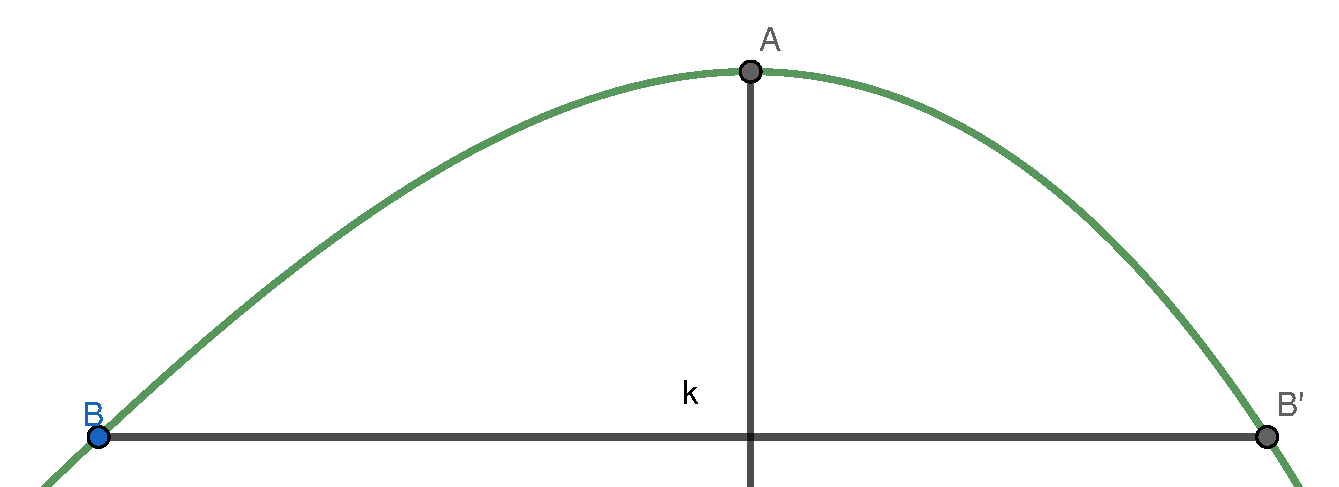
\includegraphics[scale=0.4]{2019.pdf}
        \end{center}
        Ý tưởng của câu này là sẽ xét các đoạn xoay quanh điểm cực trị của $f(x)$ thì với $B < A$ thì luôn tồn tại $B' > A$ sao cho $f(B)  = f(B')$.
        
        
        Ta xét đoạn $[a,b]$ có $a < M < b$ và $c \in (a,M)$ bất kì. Nếu như $[a,b]$ có nhiều hơn một cực trị thì ta chỉ cần co thành đoạn $a' = a + \varepsilon_1 = $ và $b' = b - \varepsilon_2$, với $0 < \varepsilon_1, \varepsilon_2 < M$ đủ lớn sao cho $f'(x) = 0$ có duy nhất nghiệm trên $[a',b']$. Khi này ta xét đến đoạn $[a',b']$. 
        
        
        Không mất tính tổng quát, giả sử đoạn có 1 cực trị $M$ là $[a,b]$, và sẵn theo câu a) thì giả sử $M = max\{f(x)\}$ trên $[a,b]$
        
        
        Đặt $g(x) = f(x) - f(c)$ thì có $g(a) < 0$ và $ g(b) > 0$ thì $g(a).g(b) < 0$, rõ ràng là $g(x)$ có nghiệm trên $(a,b)$, tức là $\exists c' \in (a,b)\backslash{c}$ sao cho $f(c) = f(c')$. 


        Giả sử rằng $c' < M$ thì khi này ta có $f'(c) = f'(c')$, theo định lý Rolle tồn tại $d$ sao cho $f'(d) = 0$, mà $d < M$ vô lý, nên vì vậy $c' \in (M,b)$. 
        
        
        Tương tự như vậy mà vì $f$ liên tục nên có vô hạn $c \in (a,M)$ đồng thời cũng sinh ra vô hạn $c' \in (M,b)$


        Nếu với mỗi $c$ và $c'$ như vậy ta đặt $x_n = c$ và $y_n = c'$ thì sẽ có $f(x_n) = f(y_n)$ với mọi $n \geq 1$. Và ta sẽ xây dựng công thức tổng quát cho $x_n$ và $y_n$.


        Phân hoạch $[a,M]$ thành $n$ đoạn thì mỗi đoạn có độ dài là $\frac{M - a}{n}$,  và ta có dãy $x_1 = a, x_n = x_{n - 1}+ \frac{M - a}{2^n} $. Khi đó đường thẳng $y = f(x_n)$ nằm ngang trên đồ thị và cắt phần $f(x)$ đoạn $(M,b]$ tại một điểm duy nhất là $y_n$.
        
        Nếu $f(a) < f(b)$ thì ta cho $a$ tiến thêm một khoảng nữa là $a'$ sao cho $f(a') > f(b)$. Và giả sử $f(a) > f(b)$.


        Khi này nếu cho $n \to +\infty$ thì $\lim x_n = M$ thì đường thẳng $y$ cũng tịnh tiến lên trên về $(M,f(M))$, chứng tỏ rằng $(y_n)$ cũng tăng và bị chặn. Khi $y$ tiếp xúc $f(x)$ duy nhất tại điểm $(M,f(M))$ trên $[a,b]$ thì cũng là khi $\lim x_n = \lim y_n = M$, và ta hoàn tất chứng minh.
    \end{comment}
    \item \begin{btvn}\vocab{(VMO 2020).}
        Cho dãy số $(x_n)$ xác định bởi: $x_1=1$ và $x_{n+1}=x_n+3\sqrt{x_n} + \frac{n}{\sqrt{x_n}}$,$\forall$n$\ge1$\\
a) Chứng minh rằng lim$\frac{n}{x_n}=0$\\ 
b) Tính lim$\frac{n^2}{x_n}$
    \end{btvn}


    \begin{comment}
        a) Vì $x_n$ là dãy dương nên ta có $\frac{n}{x_n} > 0$. Dễ dàng chứng minh $x_n > n^2$ bằng quy nạp. Thì ta có $\frac{n}{x_n} < \frac{1}{n}$. Cho $n \to +\infty$ thì theo nguyên lý kẹp, $\lim\frac{n}{x_n} = 0$ 


        b) Vì $x_n > n^2$ nên $\lim x_n = +\infty$. Áp dụng định lý Stolz ta có 
        \[\lim \frac{n}{\sqrt{x_n}} =\lim \frac{1}{\sqrt{x_{n + 1}} - \sqrt{x_n}} = \lim \frac{\sqrt{x_{n+1}} + \sqrt{x_n}}{x_{n + 1} - x_n} = \lim \frac{\sqrt{x_n + 3\sqrt{x_n} + \frac{n}{\sqrt{x_n}}}+ \sqrt{x_n}}{3\sqrt{x_n} + \frac{n}{\sqrt{x_n}}} \]
        \[
            = \lim \frac{\sqrt{\sqrt{x_n} + \frac{3}{\sqrt{x_n}} + \frac{n}{x_n\sqrt{x_n}}}+ 1}{3 + \frac{n}{x_n}} = \frac{1 + 1}{3} = \frac{2}{3}
        \]
        Vì vậy $\lim\frac{n^2}{x_n} = \frac{4}{9}$
    \end{comment}

    \item \begin{btvn}\vocab{(VMO 2021).}
        Cho dãy số $(x_n)$ xác định bởi $x_1\in (0;\frac{1}{2})$ và $x_{n+1}=3x_n^2-2nx_n^3, n\geq 1$.\\
        a) Chứng minh rằng $(x_n)$ hội tụ về $0$.

        
        b) Với mỗi $n\ge 1$, đặt $y_n=x_1+2x_2+\cdots+n x_n$. Chứng minh rằng $(y_n)$ có giới hạn hữu hạn.
    \end{btvn}

    \begin{comment}
        a) Theo bất đẳng thức AM-GM ta có $$|x_{n + 1 }| = |\frac{x_n}{2n}.(2nx_n)\left(3 - 2nx_n\right)| \leq \frac{x_n}{2n}\left(\frac{3 - 2nx_n + 2nx_n}{2}\right)^2 \leq \frac{9}{16}|x_n|, \forall n\geq 2 $$
        Suy ra $|x_{n + 1}| \leq \left(\frac{9}{16}\right)^n x_1$. Chọn $n$ đủ lớn thì có $\lim x_n = 0$


        b) Theo tiêu chuẩn d'Alembert ta xét biểu thức 
        \[D =\lim\frac{(n + 1)x_{n+1}}{nx_n} \leq \lim \frac{9}{16}\frac{n + 1}{n} = \frac{9}{16}\]
        Vì $D < 1$ nên $y_n$ có giới hạn hữu hạn.
    \end{comment}
    \item \begin{btvn}\vocab{(VMO 2022).}
        Cho $a$ là một số thực không âm và dãy số $(u_n)$ được định nghĩa như sau:
$$u_1=6, u_{n+1} = \frac{2n+a}{n} + \sqrt{\frac{n+a}{n}u_n+4}, \forall n \ge 1$$

Với $a \ge 0$, chứng minh rằng tồn tại giới hạn hữu hạn của $(u_n)$.
    \end{btvn}

    \begin{comment}
        Dự đoán $\lim u_n = 5$. Bằng quy nạp ta chứng minh được $u_n \geq 5, \forall n \geq 1$. Ta có khai triển như sau:
        \[
            |u_n - 5| \leq |\frac{2n + a}{n} - 2| + |\sqrt{\frac{n+a}{n}u_n+4} -3| \leq \frac{a}{n} + \frac{\frac{n + a}{n}|u_n - 5| + \frac{5a}{n}}{\sqrt{\frac{ n+a}{n}u_n + 4} + 3}
        \]
        \[
            \leq \frac{n + a}{6n}|u_n - 5| + \frac{5a}{6n}
        \]  
        Vì $a$ là cố định nên ta chỉ cần xét từ $n \geq \lfloor a \rfloor $ là được. Ta có 
        \[|u_n - 5| \leq \frac{1}{3}|u_n -5| + y_n, \text{ với } \lim y_n = \lim \frac{5a}{6n} = 0\]
        Áp dụng bổ đề dãy số ta được $\lim x_n = 5$.
    \end{comment}
    %\vocab{Bình luận: } \textit{Bài toán này còn có một cách làm nữa đó là ta sử dụng giải tích tương tự bài dãy số năm 2017, việc trình bày cách 2 sẽ nhường lại cho bạn đọc.}
    \item \begin{btvn}\vocab{(VMO 2023).}
        Xét dãy số $(a_n)$ thỏa mãn $a_1=\dfrac{1}{2}, a_{n+1}=\sqrt[3]{3a_{n+1}-a_n}$ và $0\le a_n\le 1, \forall n\ge 1.$

a. Chứng minh rằng dãy số $(a_n)$ được xác định duy nhất và có giới hạn hữu hạn.

b. Đặt $b_n=(1+2.a_1)(1+2^2a_2)...(1+2^na_n), \forall n\ge 1.$

Chứng minh rằng dãy số $(b_n)$ có giới hạn hữu hạn.
    \end{btvn}

    \begin{comment}
        a) Đặt $a_n = 2\sin{\alpha_n}$. Ta có $\sin{\alpha_n} = 3\frac{a_{n + 1}}{2} - \frac{4a_{n + 1}^3}{2^3} \Rightarrow a_{n + 1} = 2\sin{\frac{\alpha_n}{3}}$
        

        Thực hiện truy toán như vậy nếu đặt $a_1 = 2\sin{\alpha}$ thì ta có $a_n = 2\sin{\frac{\alpha}{3^{n-1}}}$
        

        Do đó $(a_n)$ xác định duy nhất và $\lim a_n = 0$


        b) Ta có $\frac{b_{n + 1}}{b_n} = 1 + 2^na_n > 1$ nên $(b_n)$ tăng. Mặt khác, vì $0 < \frac{\alpha}{3^{n-1}} < \frac{\pi}{2}, \forall n \geq 1$.\\ Xét $f(x) = \sin{x} - x$ trên $(0, \frac{\pi}{2})$ có $f'(x) = \cos{x} - 1 \leq 0$ nên $f(x)$ giảm và $f(x) \leq 0$.\\ Do đó ta có đánh giá $$a_n =  2\sin{\frac{\alpha}{3^{n-1}}} \leq \frac{2\alpha}{3^{n-1}}$$
        Khi này viết lại với chú ý $\ln(x + 1) \leq x, \forall x \geq 1$
        \[
            b_n \leq  \prod_{i = 1}^n \left(1 + \frac{2^{i + 1}\alpha}{3^{i - 1}}\right)
            \Leftrightarrow \ln b_n \leq \sum _{i = 1}^n  \left(1 + \frac{2^{i + 1}\alpha}{3^{i - 1}}\right) \leq \sum_{i = 1}^n 6\alpha\frac{2^i}{3^i} = 12\alpha\left(1 - \left(\frac{2}{3}\right)^n\right) \leq 12\alpha
        \]
        Suy ra được $b_n \leq e^{12\alpha}$. Nên theo Weierstrass thì $(b_n)$ hội tụ, hoàn tất chứng minh.
    \end{comment}

    \item \begin{btvn}\vocab{(VMO 2024).}
        Với mỗi số thực $x$, kí hiệu $\lfloor x \rfloor$ là số nguyên lớn nhất không vượt quá $x$.


Dãy số $\{a_n \}_{n=1}^{\infty}$ được định nghĩa bởi $a_n = \frac{1}{4^{\lfloor -\log_4 n \rfloor}}, \forall n \geq 1.$ Đặt $b_n = \frac{1}{n^2} \left( \sum_{k=1}^n a_k - \frac{1}{a_1+a_2} \right).$

a) Tìm đa thức $P(x)$ với hệ số thực sao cho $b_n = P \left( \frac{a_n}{n} \right), \forall n \geq 1$.\\
b) Chứng minh rằng tồn tại một dãy số tăng nghiêm ngặt $\{n_k \}_{k=1}^{\infty}$ của các số nguyên dương sao cho$$\lim_{k \to \infty} b_{n_k} = \frac{2024}{2025}.$$
    \end{btvn}

    \begin{comment}
        a) Mỗi lần $n$ tăng gấp 4 lần thì $a_n$ cũng tăng gấp 4 lần, nếu không thì các số hạng kề $a_n$ không đổi. Vậy nên với mỗi $n$, $\exists t: 4^t \leq n \leq 4^{t + 1}$ và $a_n = 4^t$.\\
        Ta để ý rằng $a_1 = 1$, $a_2,a_3,a_4 = 4$, $a_5,a_6,...,a_{16} = 16$ và ta có lập luận rằng cứ mỗi $a_{4^{k-1} + 1},a_{4^{k-1} + 2},...,a_{4^k}$ thì giá trị vẫn giữ nguyên, và cứ một cụm như thế thì sẽ có tổng là $T_k = (4^{k} - (4^{k-1} + 1) + 1)4^k = 12.16^{k-1}$.


        Ta đặt $n = 4^m + r$ trong đó $m$ là số lớn nhất sao cho $4^m \leq n$ và $m,r \in \mathbb{Z}^+$. Tất nhiên là ta được $r = n - a_n$. Khi đó có 
        \[S = \sum_{i = 1}^{4^m + r} a_i = \sum_{i = 1}^{4^m}a_i + \sum_{i = 4^m + 1}^{4^m + r} a_n = 1 + \sum_{i = 0}^{m} T_i + a_n.r = 1 + \sum_{i = 0}^{m} 12.16^{i} + a_n(n - a_n)\]\[ = 1 + 4\frac{16^m - 1}{5}  + na_n - a_n^2 = 1 + \frac{4a_n^2 - 4}{5} +na_n -a_n^2 = -\frac{1}{5}a_n^2 + na_n + \frac{1}{5}\]
        Khi này thay $S$ vào $b_n$ ta được 
        \[b_n = \frac{1}{n^2}\left(S - \frac{1}{5}\right) = -\frac{1}{5}.\frac{a_n^2}{n^2} + \frac{a_n}{n} = P\left(\frac{a_n}{n}\right)\]
        Khi này ta có được $P(x) = -\frac{1}{5}x^2 + x$, hoàn tất câu a).


        b) Để giải quyết được câu b) thì ta hãy tìm hiểu một khái niệm khác trong \vocabf{tiền giải tích (Precalculus)} là \vocabf{Tập hợp trù mật}.

        
        \vocab{- Định nghĩa 9: } Một tập con $A$ trong $X$ được gọi \vocabf{trù mật (hoặc dày đặc)} trong $X$ nếu mọi điểm trong $X$ hoặc là thuộc $X$ hoặc gần tùy ý với một phần tử của $A$.


        Ta có một định lý khá quan trọng như sau:
        \begin{theo}[Định lý trù mật]
            -Với $a < b$ là hai số thực bất kì thì luôn tồn tại số hữu tỉ $q$ sao cho $a < q < b$.
        \end{theo}
        \vocab{Chứng minh: }Đặt $c = b - a > 0$. Khi đó tồn tại số nguyên dương $n$ sao cho $0 < \frac{1}{n} < c$. Điều này không phải hiển nhiên, ta có tiên đề sau
        \begin{theo}[Tiên đề Archimedes]
            -Cho $x,y$ là hai số thực dương, khi đó tồn tại số nguyên dương $m$ sao cho $mx > y$
        \end{theo}
        Cách chứng minh tiền đề này phải dùng đến \vocabf{lý thuyết topo} rất phức tạp nên ta hãy tạm thời thừa nhận nó mà không chứng minh lại.



        Chọn $x = c$ và $y = 1$ thì khẳng định trên đúng. Giờ ta xét các số hữu tỉ dạng $\frac{m}{n}$ với $m \in \mathbb{Z}$ và $n$ nguyên dương cố định. Cũng theo tiên đề Archimedes, luôn tồn tại số hữu tỉ $\frac{m_1}{n} < a$  và số hữu tỉ $\frac{m_2}{n} > b$


        Như vậy ta xét các số hữu tỉ $\frac{m_1}{n}, \frac{m_1 + 1}{n},...\frac{m_2 - 1}{n},\frac{m_2}{n}$. Đặt $p$ là số nguyên lớn nhất sao cho $\frac{p}{n} \leq a$. Khi đó có $a < \frac{p + 1}{n} < b$, hoàn tất chứng minh.


        Mở rộng sang ngôn ngữ dãy số thì điều này cho ta một hệ quả vô cùng quan trọng như sau: 
        \begin{theo}[Hệ quả 1]
            -Nếu $a < b$ là hai số thực dương thì tồn tại vô hạn số hữu tỉ thuộc $(a,b)$. Hay nói cách khác luôn tồn tại dãy $(s_n)$ hữu tỉ với $a < s_n < b, \forall n \geq 1$ và $\lim s_n = L$ với $L$ tùy ý thuộc $(a,b)$.
        \end{theo}
        Và ta còn có thể có một hệ quả thứ hai nữa là
        \begin{theo}[Hệ quả 2]
            -Nếu $(a_n)$ là dãy thực có các phần tử thuộc tập $T$ trù mật trên khoảng nào đó thì tồn tại một dãy $s_n$ nguyên dương tăng ngặt sao cho $\lim a_{s_n} = L$ với $L$ thuộc $T$ tùy ý.
        \end{theo}
        Quay trở lại bài toán, ta có $P(1) = \frac{4}{5} < \frac{2024}{2025} < P(2) = \frac{6}{5}$, cho nên vì tính liên tục của $P$ nên tồn tại $\alpha \in (1,2)$ sao cho $P(\alpha) = \frac{2024}{2025}$. Như vậy bài toán sẽ hoàn tất nếu ta chỉ ra được tập hợp 
        \[T = \left\{\frac{4^{i + 1}}{4^i + r} | i,r \in \mathbb{N}, 0 < q \leq 3.4^i\right\}\]
        trù mật trên $(1,2)$. Với $a < b \in (1,2)$ bất kì thì luôn tồn tại số $i,r$ sao cho $$ a < \frac{4^{i + 1}}{4^i + r} < b \Leftrightarrow \frac{a}{4^{i + 1}} < \frac{1}{4^i + r} < \frac{b}{4^{i + 1}} \Leftrightarrow 4^i(\frac{4}{b} - 1) < r < 4^i(\frac{4}{a} - 1) \Leftrightarrow 4^i(\frac{4}{a} - \frac{4}{b}) > 1$$  nếu chọn $i$ đủ lớn, dẫn tới sự tồn tại của $r$, vậy nên $T$ trù mật trên $(1,2)$. 

        
        
        Viết $n = 4^m + r$ thì ta được $\frac{a_n}{n} = \frac{4^{m + 1}}{4^m + r} \in T$. Theo hệ quả trù mật thì vì đã có $\left(\frac{a_n}{n}\right)$ là dãy hữu tỉ nên phải tồn tại dãy $(n_k)$ nguyên dương tăng ngặt để $\displaystyle \lim_{k \to +\infty}\frac{a_{n_k}}{n_k} = P(\alpha) = \frac{2024}{2025}$, hoàn tất chứng minh.
    \end{comment}
    \item \begin{btvn}\vocab{(OLP 30/4 2024).}
        Cho dãy số $(x_n)$ được xác định bởi $$x_1 = 1, x_{n + 1} = \frac{1 + \sqrt{1 + x_n^2} - x_n}{1 + \sqrt{ 1 + x_n^2} + x_n}$$Chứng minh rằng $(x_n)$ có giới hạn hữu hạn và tìm giới hạn đó.
    \end{btvn}

    \begin{comment}
        \vocab{Cách 1: Sử dụng bổ đề dãy số.} Viết lại ta có $x_{n + 1} = \sqrt{x_n^2 + 1} - x_n$. Dự đoán $\lim x_n = \frac{1}{\sqrt{3}}$. Lại có 
        $x_{n + 1} = \frac{1}{\sqrt{x_n^2 + 1} + x_n} > 0$ nên cũng có $x_{n+ 1} \leq 1$
        \[(x_{n + 1} - \frac{1}{\sqrt{3}}) = \sqrt{x_n^2 + 1} - \frac{2}{\sqrt{3}} - (x_n - \frac{1}{\sqrt{3}}) = \frac{(x_n + \frac{1}{\sqrt{3}})(x_n - \frac{1}{\sqrt{3}})}{\sqrt{x_n^2 + 1} + \frac{2}{\sqrt{3}}} \leq (\sqrt{3} - 1)(x_n - \frac{1}{\sqrt{3}})
        \]
        \[\Leftrightarrow |x_{n + 1} - \frac{1}{\sqrt{3}}| \leq (2 - \sqrt{3})|x_n - \frac{1}{\sqrt{3}}|\]
        Áp dụng bổ đề dãy số thì $(x_n)$ có giới hạn hữu hạn và $\lim x_n = \frac{1}{\sqrt{3}}$ 


        \vocab{Cách 2: Sử dụng lượng giác.} Đặt $x_n = \tan{x}$. Ta có 
        \[x_{ n + 1} = \sqrt{\tan^2{x} + 1} - tan{x} = \frac{1}{\cos x} - \tan{x} = \frac{\sin{\frac{\pi}{2}} - \sin{x}}{cos{x}} = \frac{2\cos(\frac{\pi}{4} + \frac{x}{2})\sin(\frac{\pi}{4} -\frac{x}{2})}{\sin(\frac{\pi}{2} - x)}\]
        \[
        = \frac{\cos(\frac{\pi}{4} + \frac{x}{2})}{\cos(\frac{\pi}{4} - \frac{x}{2})} = \tan(\frac{\pi}{4} - \frac{x}{2})
        \]
        Khi đó ta sẽ quy nạp được $x_n = \tan\left(\frac{\pi}{6} + \frac{\pi}{12}\left(-\frac{1}{2}\right)^{n - 1}\right)$. Vậy nên $\lim x_n = \frac{1}{\sqrt{3}}$
    \end{comment}
    \item \begin{btvn}\vocab{(IMC 2015). }
    Cho hệ thức truy hồi được xác định bởi $F(0)=0$, $F(1)=\frac32$, và $F(n)=\frac{5}{2}F(n-1)-F(n-2)$
    for $n\ge2$.
    
    Chứng minh rằng $\displaystyle{\sum_{n=0}^{\infty}\,
        \frac{1}{F(2^n)}}$ là một số hữu tỉ.
    \end{btvn}

    \begin{comment}
        Xét phương trình đặc trưng có $\lambda^2 - \frac{5}{2}\lambda + 1 = 0 \Leftrightarrow \lambda = 2$ hoặc $\lambda = \frac{1}{2}$, khi đó 
        \[
            F(n) = c_1.2^n + c_2. 2^{-n}
        \]
        Cho $n = 0$ và $n = 1$ rồi giải hệ phương trình, ta tìm được $c_1 = 1$ và $c_2 = -1$, do đó $F(n) = 2^n - 2^{-n}$. Đặt $x_n = 2^{2^n}$, khi đó ta được $F(2^n) = x_n - x_n^{-1}$. Mặt khác $x_{n + 1} = x_n^2$ nên
        \[
            \frac{1}{F(2^n)} = \frac{x_n}{x_n^2-1} = \frac{x_n+1}{x_n^2-1}-\frac{1}{x_n^2-1} = \frac{1}{x_n-1}-\frac{1}{x_{n+1}-1}.
        \]
        Khi đó tổng này hội tụ về $1$ là số hữu tỉ.
    \end{comment}

    \item \begin{btvn}\vocab{(Đồng Tháp TST 2024). }
        Cho dãy số thực $(x_n)$ có $x_1 = 2$ và
        \[x_{n + 1} = \frac{n^2- 1}{x_n} + 2, \forall n \geq 1\]


        a) Chứng minh rằng $\lim x_n = +\infty$


        b) Xét dãy $(y_n)$ được xác định bởi
        \[y_n = \frac{x_1}{1.2^1} + \frac{x_2}{2.2^2} + \dots + \frac{x_n}{n.2^n}\]
        Chứng minh rằng $(y_n)$ có giới hạn hữu hạn và $\lim y_n < 2$.
        
    \end{btvn}

    \begin{comment}
        a) Ta sẽ chứng minh quy nạp rằng $n \leq x_n \leq n + 1, \forall n \geq 1$. Với $x_1$ thì hiển nhiên đúng, giả sử mệnh đề đúng với $x_n$, ta có 
        \[x_{n + 1} \geq \frac{n^2 - 1}{n + 1} + 2 = n + 1\]
        \[x_{n + 1} \leq \frac{n^2 - 1}{n} + 2 = n - \frac{1}{n} +2 \leq n + 2\]
        Vậy nên mệnh đề quy nạp là đúng. Lại có $x_n \geq n$ nên $\lim x_n = +\infty$.


        b) Dễ thấy rằng $y_n$ là dãy tăng. Trước tiên ta xét chứng minh bxất đẳng thức sau đúng $ 2^{n - 1} > n, \forall n \geq 3$. Xét $f(x) = 2^{x - 1} - x$ trên $[3,+\infty)$ có $f'(x) = \ln2.2^{x - 1} - 1 > 0, \forall n \geq 3$. Vậy nên $f(x)$ tăng và $f(x) > f(3) = 1 > 0$ nên vì vậy $2^n > 2n, \forall n \geq 3$.
        
        
        Áp dụng đánh giá này đồng thời với $ 2^{n - 1} \geq n, \forall n < 3$, ta có 
        $$
        y_n = \sum_{i = 1}^n \frac{x_i}{i.2^i} \leq \sum_{i = 1}^n \frac{i + 1}{i.2^i} = 
        \sum_{i = 1}^n \frac{1}{2^i} + \frac{1}{i.2^i} < 1 - \frac{1}{2^{n}}+ \sum_{i = 1}^n \frac{1}{2i^2}
        $$
        Ta có đẳng thức tổng nghịch đảo bình phương là $\displaystyle \sum_{i = 1}^{\infty} \frac{1}{i^2} = \frac{\pi^2}{6}$, tương đương $\displaystyle \sum_{i = 1}^{n} \frac{1}{i^2} < \frac{\pi^2}{6}, \forall n \geq 1$ nên ta được
        \[y_n \leq 1 + \frac{\pi^2}{12} \]
        Suy ra $(y_n)$ bị chặn trên. Theo Weierstrass thì $(y_n)$ hội tụ và ta có được $\lim y_n \leq 1 + \frac{\pi^2}{12} < 2$
    \end{comment}

        \begin{comment}\vocab{Bình luận: } \textit{Trong bài toán trên thì ta đã sử dụng một đẳng thức rất nổi tiếng được Euler chứng minh khi ông 28 tuổi, ta phát biểu lại như sau:}


        \begin{theo}[Đẳng thức tổng nghịch đảo bình phương]
            -Cho $n$ là số thực dương lớn hơn 1, khi đó
            \[\sum_{i = 1}^{\infty} \frac{1}{i^2} = \frac{1}{1^2} + \frac{1}{2^2} + \frac{1}{3^2} + ... = \frac{\pi^2}{6}
            \]
        \end{theo}
        \textit{Để chứng minh đẳng thức này, ta sẽ sử dụng một khái niệm giải tích khác là Khai triển Taylor.}

        \begin{theo}[Khai triển Taylor]
            -Giả sử hàm số $f(x)$ có đạo hàm cấp tùy ý tại điểm $x_0$, khi này ta có 
            \[f(x) = f(x_0) + \frac{f'(x_0)}{1!} + \frac{f''(x_0)}{2!} + \frac{f'''(x_0)}{3!} + ... + \frac{f^{(n)}x_0}{n!} + ...= \sum_{i = 0}^{\infty} \frac{f^{(i)}(x_0)}{i!} \]
        \end{theo}
        \textit{Thông thường để thuận tiện thì ta xét khai triển tại điểm $x_0 = 0$, lúc này khai triển còn có tên gọi khác là Khai triển Maclaurin.}


        Quay trở lại bài toán, xét khai triển Maclaurin của $f(x) = \sin(x)$ như sau:
        \[
        f(x) = x - \frac{x^3}{3!} + \frac{x^5}{5!} - \frac{x^7}{7!} + ...\tag{1}
        \]
        Mặt khác, phương trình $\sin(x) = 0$ có các nghiệm là $\{0 , \pm \pi, \pm 2\pi,\pm 3\pi,...\}$, nên từ đó có
        \[\sin(x) = Cx(x^2 - \pi^2)(x^2 - 2^2\pi^2)(x^2 - 3^2\pi^2)... \tag{2}\]
        Từ (1) và (2) ta được   
        \[1 - \frac{x^2}{3!} + \frac{x^4}{5!} - \frac{x^6}{7!} + ... = C(x^2 - \pi^2)(x^2 - 2^2\pi^2)(x^2 - 3^2\pi^2)...
        \] Vì $C$ là hằng số tùy ý nên ta có 
        \[VP = (1 - \frac{x}{\pi^2})(1 - \frac{x}{2^2\pi^2})(1 - \frac{x}{3^2\pi^2})...\]
        Đồng nhất hệ số ta được
        \[-\frac{x}{3!} =-\frac{x}{\pi^2} -\frac{x}{2^2\pi^2} -\frac{x}{3^2\pi^2} -...\]
        \[\Leftrightarrow \frac{1}{1^2} + \frac{1}{2^2} + \frac{1}{3^2} + ... = \frac{\pi^2}{6}\]
    \end{comment}
        \item \begin{btvn}\vocab{(TST Bắc Ninh 2018). }
            Cho dãy số $\left(x_n\right)$ được xác định bởi $$x_0=2017, x_n=-\frac{2017}{n} \sum_{k=0}^{n-1} x_k(n \geq 1)$$ Tìm giới hạn
\[
L=\lim \frac{n^2 \cdot\displaystyle \sum_{k=0}^{2017} 2^k x_k+5}{-2018 n^2+4 n-3} .
\]
        \end{btvn}
        \begin{comment}
        Tương tự bài VMO 2011, chỉ xét riêng với $n \leq 2017$, ta có được
        \[
        x_{n} = -x_{n - 1} \frac{2018 - n}{n} = x_{n -2} \frac{(2018 - n)(2018 -(n - 1))}{n(n -1)} = ... = \frac{(-1)^nA_{2017}^{n - 1}}{n!} = (-1)^n \binom{2017}{n - 1}
        \]
        Khi đó 
        \[
            \displaystyle \sum_{i=0}^{2017} 2^k x_i = \displaystyle \sum_{i=0}^{2017} (-2)^i .1^{2017 - i}\binom{2017}{n - 1} = (1 - 2)^{2017} = -1
        \]
        Vì vậy $L = \frac{1}{2018}$
        \end{comment}
        \subsection{\LARGE \textcolor{dk}{Lời giải}}
    \newpage
    \thispagestyle{plain}
    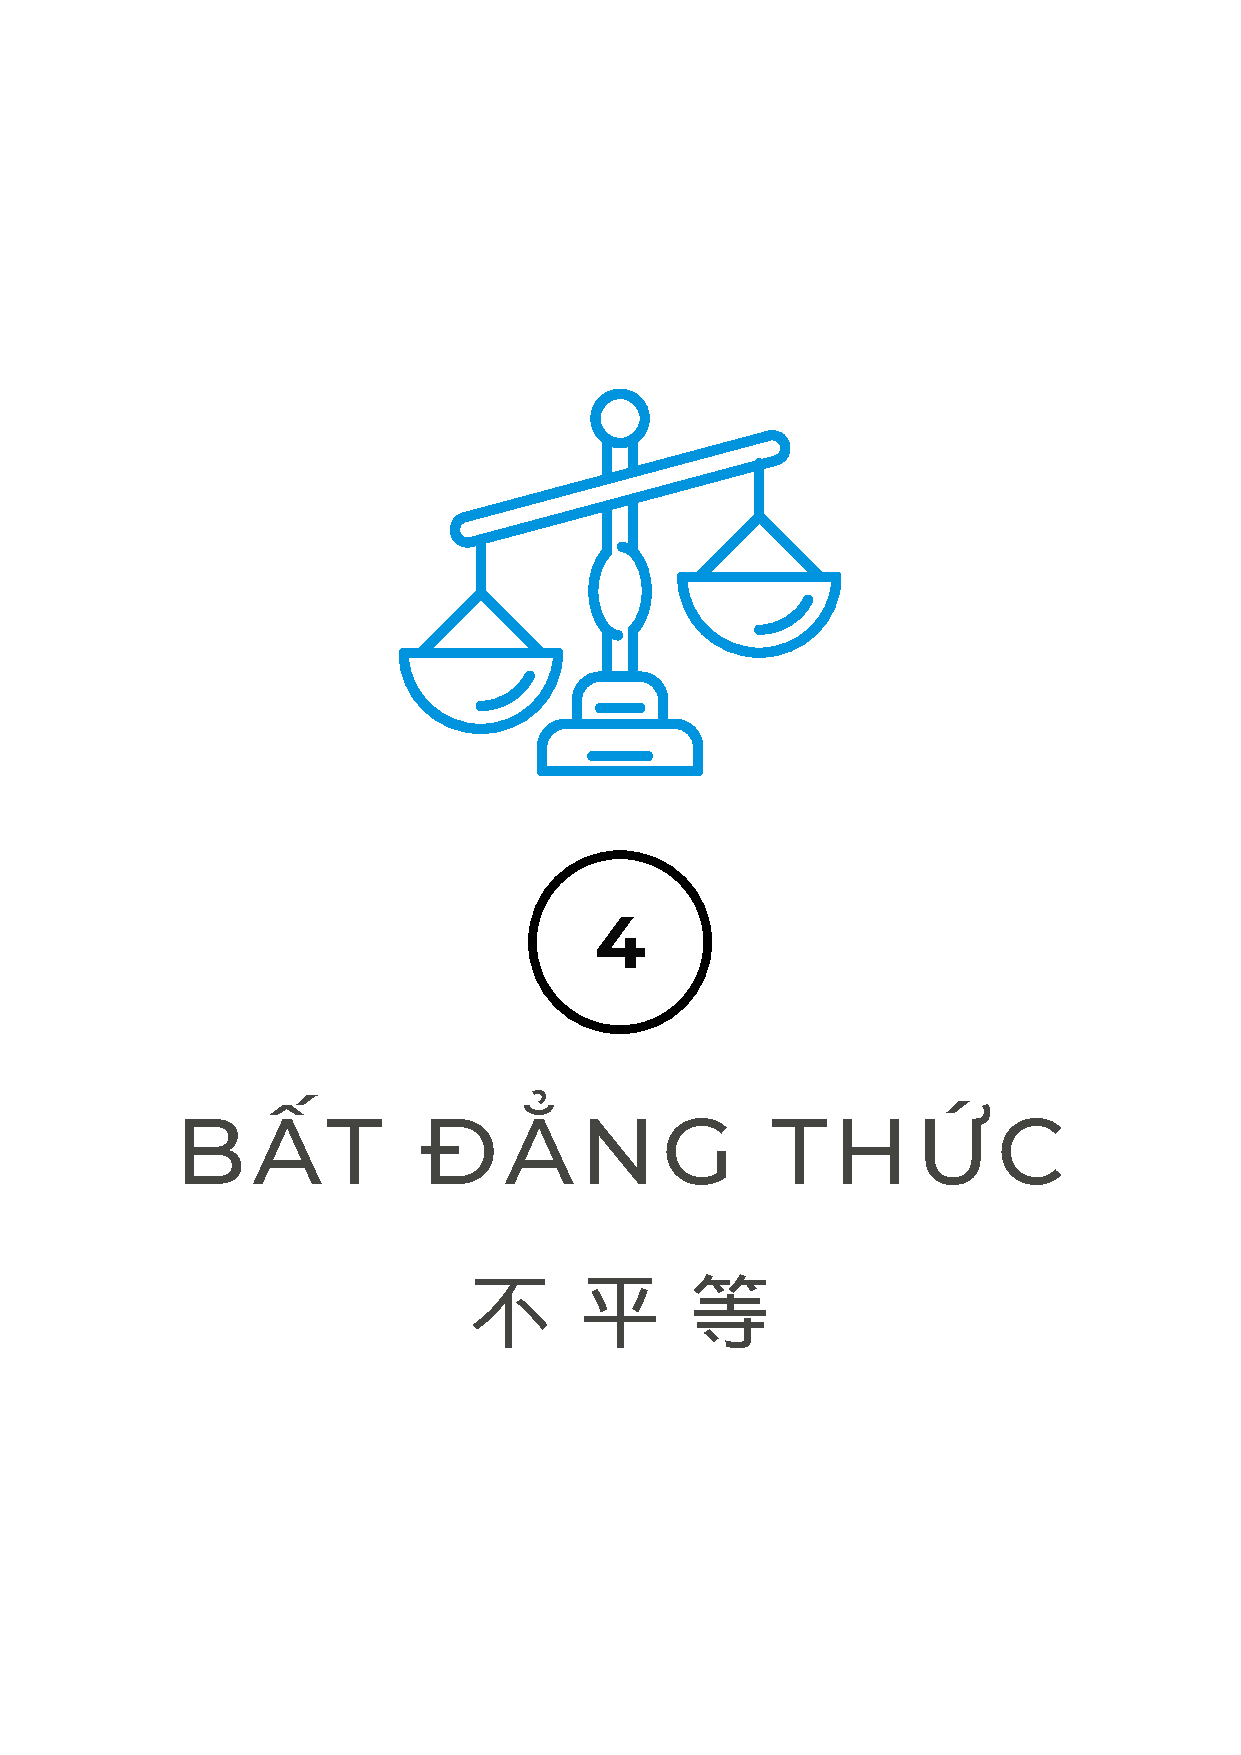
\includepdf[pages=1]{4.pdf}
    \section{\huge Bất đẳng thức}
    \subsection{\LARGE \textcolor{dk}{Đề bài}}
        \item \begin{btvn}\vocab{(Taiwan TST 2014).}
            Cho $a,b,c >0$. Chứng minh rằng
            \[
                3(a + b + c) \geq 8\sqrt[3]{abc} + \sqrt[3]{\frac{a^3 + b^3 + c^3}{3}}
            \]
        \end{btvn}
        \item \begin{btvn} Cho $a,b,c > 0$. Chứng minh rằng 
        \[
            \frac{a}{\sqrt{b + c}} + \frac{b}{\sqrt{c + a}} + \frac{c}{\sqrt{a + b}} \geq \sqrt{\frac{3}{2}(a + b + c)}
        \]
    \end{btvn}
        \item \begin{btvn}\vocab{(Japan MO 1997).}
            Cho $a,b,c >0$. Chứng minh rằng
            \[
                \frac{(b + c - a)^2}{a^2 + (b + c)^2} + \frac{(c + a - b)^2}{b^2 + (c + a)^2} + \frac{(a + b - c)^2}{c^2 + (a + b)^2} \geq \frac{3}{5}
            \]
        \end{btvn}
        \item \begin{btvn}\vocab{(IMO 2001).}
            Cho $a,b,c >0$. Chứng minh rằng
            \[
                \frac{a}{\sqrt{a^2 + 8bc}} + \frac{b}{\sqrt{b^2 + 8ca}} + \frac{c}{\sqrt{c^2 + 8ab}} \geq 1
            \]
        \end{btvn}
        \item \begin{btvn}\vocab{(IMOSL 2009).}
            Cho $a,b,c >0$ thỏa mãn $\frac{1}{a} + \frac{1}{b} + \frac{1}{c} = a + b + c$
            \[
                \frac{1}{(2a + b + c)^2} + \frac{1}{(2b + c + a)^2} + \frac{1}{(2c + a + b)^2} \leq \frac{3}{16}
            \]
        \end{btvn}
        \item \begin{btvn}\vocab{(ELMOSL 2013).}
            Cho $a,b,c >0$ thỏa mãn $a + b + c = 3$. Chứng minh rằng
            \[
                \frac{18}{(3 -a )(4 - a)} + \frac{18}{(3 -b)(4 - b)} + \frac{18}{(3 -c )(4 - c)} + 2(ab + bc + ca) \geq 15
            \]
        \end{btvn}
        \item \begin{btvn}\vocab{(Canada MO 2002).}
            Cho $a,b,c >0$. Chứng minh rằng
            \[
                \frac{a^3}{bc} + \frac{b^3}{ca} + \frac{c^3}{ab} \geq a + b  +c
            \]
        \end{btvn}
        \item \begin{btvn}\vocab{(USAJMO 2012).}
            Cho $a,b,c >0$. Chứng minh rằng
            \[
                \frac{a^3 + 3b^3}{5a + b} + \frac{b^3 + 3c^3}{5b + c} + \frac{c^3 + 3a^3}{5c + a} \geq \frac{2}{3}(a^2 + b^2 + c^2)
            \]
        \end{btvn}
        \item \begin{btvn}\vocab{(IMO 2000).}
            Cho $a,b,c >0$ thỏa mãn $abc = 1$. Chứng minh rằng
            \[
                \left(a - 1 + \frac{1}{b}\right)\left(b - 1 + \frac{1}{c}\right)\left(c- 1 + \frac{1}{a}\right) \leq 1
            \]
        \end{btvn}
        \item \begin{btvn}\vocab{(ELMO 2003).}
            Cho $x,y,z > 1$ thỏa mãn $\frac{1}{x^2 - 1} + \frac{1}{y^2 - 1} + \frac{1}{z^2 - 1} = 1$. Chứng minh rằng
            \[
                \frac{1}{x + 1} + \frac{1}{y + 1} + \frac{1}{z + 1} \leq 1
            \]
        \end{btvn}
        \item \begin{btvn}\vocab{(USAMO 2003).}
            Cho $a,b,c >0$. Chứng minh rằng
            \[
                \frac{(2a + b + c)^2}{2a^2 + (b + c)^2} + \frac{(2b + c + a)^2}{2b^2 + (c + a)^2} + \frac{(2c + a + cb)^2}{2c^2 + (a + b)^2} \leq 9
            \]
        \end{btvn}
        \item \begin{btvn}\vocab{(USAMO 2017).}
            Cho $a,b,c,d \geq 0$ thỏa mãn $a + b + c + d = 4$. Tìm giá trị nhỏ nhất của
            \[
                \frac{a}{b^3 + 4} + \frac{b}{c^3 + 4} + \frac{c}{d^3 + 4} + \frac{d}{a^3 + 4}
            \]
        \end{btvn}

        \item \begin{btvn}\vocab{(USAMO 2004).}
            Cho $a,b,c >0$. Chứng minh rằng
            \[
                (a^5 - a^2 + 3)(b^5 - b^2 + 3)(c^5 - c^2 + 3) \geq (a + b + c)^3
            \]
        \end{btvn}
        \item \begin{btvn}\vocab{(TSTST 2012).}
            Cho $x,y,z >0$ thỏa mãn $xyz + xy + yz + zx  = x + y + z + 1$. Chứng minh rằng
            \[
                \frac{1}{3}\left(\sqrt{\frac{1 + x^2}{1 + x}} + \sqrt{\frac{1 + y^2}{1 + y}} + \sqrt{\frac{1 + z^2}{1 + z}}\right) \leq \left(\frac{x + y + z}{3}\right)^{5/8}
            \]
        \end{btvn}
        \item \begin{btvn}\vocab{(ELMO 2013).}
            Cho $a,b,c > 0$ thỏa mãn $a + b + c = \sqrt[7]{a} + \sqrt[7]{b} + \sqrt[7]{c}$. Chứng minh rằng $a^ab^bc^c \geq 1$.
        \end{btvn}
        \item\begin{btvn}
            Cho $a,b,c$ là độ dài 3 cạnh tam giác thỏa mãn $a^2 + b^2 + c^2 = 3$. Chứng minh rằng
            \[
                \frac{a}{\sqrt{b + c -a}} + \frac{b}{\sqrt{c + a -b}} + \frac{c}{\sqrt{a + b -c}} \geq 3
            \]
            
        \end{btvn}
        \begin{comment}
            Xét các biểu thức
            \[
                A =\sum_{cyc} \frac{a}{\sqrt{b + c -a}}, B = \sum_{cyc}a(b + c -a)
            \]
            Theo bất đẳng thức Holder ta có 
            \[A.A.B \geq (a + b + c)^3\]
            Ta cần chứng minh $(a + b + c)^3 \geq 9B \lra (a + b + c)^3 \geq 9\displaystyle \sum_{cyc}2ab - a^2$. Theo phép đặt $PQR$ tương tự bài trên ta có 
            \[p^3 \geq 9(2q - p^2 + 2q)
            \lra p^3 \geq 36q - 9p^2 \lra 9(p^2 -3q) + (p^3 - 9r) \geq 0
            \]
            Hiển nhiên đúng theo Schur. Vậy nên $A \geq 3$ và ta có điều phải chứng minh.
        \end{comment}
        \item\begin{btvn}
            Cho $a,b,c > 0$ có $abc = 1$. Chứng minh rằng
            \[
                \frac{a}{\sqrt{b + c + 7}} + \frac{b}{\sqrt{c + a + 7}} + \frac{c}{\sqrt{a + b + 7}} \geq 1
            \]
        \end{btvn}
        \begin{comment}
            Xét các biểu thức 
            \[
                A = \sum_{cyc}\frac{a}{\sqrt{b + c + 7}}, B = \sum_{cyc} a(b + c + 7) = \sum_{cyc} 2bc + 7a
            \]
            Theo bất đẳng thức Holder ta có 
            \[
                A^2B \geq (a + b + c)^3
            \]
            Ta cần chứng minh
            \[
                (a + b + c)^3 \geq \sum_{cyc}2bc + 7a
            \]
            Theo phép đặt PQR ta được
            \[
                p^3 \geq 2q + 7p \lra p^3 - 2q - 7p \geq 0
            \]
            Ta có $VT \geq p^3 -\frac{2}{3}p^2 - 3p = p(p^2 - \frac{2}{3}p - 3) \geq 0$ vì $p^3 \geq 27r \lra p \geq 3$. Vậy nên $A \geq 1$ và ta có điều phải chứng minh.
        \end{comment}
        \item\begin{btvn}
            Cho $a,b,c \geq 0$ thỏa mãn $ab + bc + ca > 0$. Chứng minh rằng
            \[\sqrt{\frac{a}{b + c}} + \sqrt{\frac{b}{c + a}}+ \sqrt{\frac{c}{a+ b}} \geq 2
            \]
        \end{btvn}
        \begin{comment}
            Xét các biểu thức
            \[
                A = \sum_{cyc} \sqrt{\frac{a}{b + c}},
                B = \sum_{cyc} a^2( b + c)
            \]
            Áp dụng bất đẳng thức Holder, ta có
            \[
                A.A.B \geq (a + b + c)^3
            \]
            Ta cần chứng minh $(a + b + c)^3 \geq 4B$. Theo phép đặt PQR, ta có
            \[
                p^3 \geq 4(pq - 3r) \lra (p^3 - 4pq + 9r) + 3r \geq 0
            \]
            Điều này luôn đúng theo bất đẳng thức Schur, hoàn tất bài toán.
        \end{comment}
    
        \item\begin{btvn}
            Cho $a,b,c > 0$ thỏa mãn $a^2 + b^2 + c^2 = a + b + c$. Chứng minh rằng 
            \[
                a^2b^2 + b^2c^2 + c^2a^2 \leq ab + bc + ca
            \]
        \end{btvn}
        \begin{comment}
            Ta có 
            \[
                (a^2 + b^2 + c^2)^2 = (a + b + c)^2 \lra \sum_{cyc}a^4 + 2b^2c^2 = \sum_{cyc}a^2 + 2bc
            \]
            Vậy nên ta cần chứng minh $a^4 + b^4 + c^4 \geq a^2 + b^2 + c^2$. Áp dụng bất đẳng thức Holder ta được
            \[
                (a^4 + b^4 + c^4)(a + b + c)^2 \geq (a^2 + b^2 + c^2)^3 \lra a^4 + b^4 + c^4
            \]
            Hoàn tất bài toán.
        \end{comment}
        
    
    
        \item\begin{btvn}
            Cho $a,b,c > 0$. Chứng minh rằng
            \[\sqrt{\frac{a + b}{c}} + \sqrt{\frac{b + c}{a}} + \sqrt{\frac{c + a}{b}} \geq 4(a +b + c)\sqrt{\frac{a + b + c}{3(a + b)(b + c)(c + a)}}
            \]
        \end{btvn}
        \begin{comment}
        Sử dụng bất đẳng thức Holder ta có 
            \[
                \left(\sum_{cyc}c(a+b)^2\right)\left(\sqrt{\frac{a + b}{c}} + \sqrt{\frac{b + c}{a}} + \sqrt{\frac{c + a}{b}}\right)^2 \geq 8(a + b +c)^3
            \]
            Ta cần chứng minh 
            \[
                    8(a + b + c)^3 \geq 16\frac{(a + b + c)^3}{3(a + b)(b + c)(c + a)} \left(\sum_{cyc}c(a+b)^2\right)
            \]
            \[
                \lra 3(a + b)(b + c)(c + a) \geq 2 \left(\sum_{cyc}c(a+b)^2\right)
            \]
            Chuẩn hóa $a + b + c = 3$, ta có 
            \[
                3(3 - a)(3 - b)(3 - c) \geq 2\left(\sum_{cyc}a(3-a)^2\right) = 2\sum_{cyc}a^3 - 6a^2 + 9a \tag{1}
            \]
            Theo phép đặt PQR, ta có các biểu thức sau:
                \begin{align*}
                    &(3 - a)(3 - b)(3 - c) = 3q - r\\
                    &a^2 + b^2 + c^2 = 9 -2q\\
                    &a^3 + b^3 + c^3 = p^3 - 3pq + 3r = 27 - 9q + 3r
                \end{align*}
                Từ đó ta được
            \[
                (1) \lra 9q - 3r \geq 2(27 - 9q + 3r - 54 + 12q +27) = 2(3q +3r) \lra q \geq 3r
            \]
            bất đẳng thức này luôn đúng vì $ r \leq \frac{pq}{9} \lra q \geq 3r$. Từ đó cho ta điều phải chứng minh.
            \end{comment}
            \item\begin{btvn}
                Cho $a,b,c > 0$ có $a + b + c = 1$. Chứng minh rằng
                \[
                    \frac{a}{\sqrt{b + c}} + \frac{b}{\sqrt{c + a}} + \frac{c}{\sqrt{a + b}} \geq \sqrt{\frac{3}{2}}
                \]
            \end{btvn}
            \begin{comment}
                Sử dụng bất đẳng thức Holder ta được
                \[
                    \left(\sum_{cyc}a^2(b + c)\right)\left(\sum_{cyc}\frac{a}{\sqrt{b + c}}\right)^2 \geq (a + b + c)^3
                \]
                Ta cần chứng minh 
                \[
                    (a + b + c)^3 \geq  \frac{3}{2}\left(\sum_{cyc}a^2(b + c)\right) \lra 2 \geq 3\sum_{cyc}a^2(1 -a) = 3(q - 3r) \lra 3q \leq 9r + 2
                \]
                Lại có $9r \leq q$ nên tương đương $3q \leq 9r + 2 \leq q + 2 \lra q \leq 1$. Điều này rõ ràng đúng, nên từ đó cho ta điều phải chứng minh.
            \end{comment}
            \item\begin{btvn}
                Cho $a,b,c > 0$ có $a + b + c = 1$. Chứng minh rằng
                \[
                    4abc\left[\frac{a}{(a + 1)^2} + \frac{b}{(b + 1)^2} + \frac{c}{(c + 1)^2}\right] + 1 \geq \frac{13}{4}(ab + bc + ca)
                \]
            \end{btvn}
            \begin{comment}
                Ta sẽ cần chứng minh 2 bất đẳng thức nhỏ sau:
                \[
                \left\{
                    \begin{array}{l}
                        (a + b + c)^2 \geq 3(ab + bc + ca)\\
                        \frac{a}{(a + 1)^2} + \frac{b}{(b + 1)^2} + \frac{c}{(c + 1)^2}\geq \frac{1}{16}\left(\frac{1}{a} + \frac{1}{b} + \frac{1}{c}\right)
                    \end{array}
                \right.\]
                bất đẳng thức thứ nhất hiển nhiên đúng theo bất đẳng thức Schur. Ta quan tâm đến bất đẳng thức thứ 2. Sử dụng bất đẳng thức Holder ta có 
                \[
                    \left(\sum_{cyc}a(a + 1)\right)^2\left[\frac{a}{(a + 1)^2} + \frac{b}{(b + 1)^2} + \frac{c}{(c + 1)^2}\right] \geq (a + b + c)^3
                \]
                Ta cần chứng minh $\displaystyle (a + b + c)^3 \geq \frac{1}{16}\left(\sum_{cyc}a(a + 1)\right)^2\left(\frac{1}{a} + \frac{1}{b} + \frac{1}{c}\right)$. Theo phép thế PQR ta có
                \[
                    1 \geq \frac{q^2}{4}.\frac{q}{r} \lra 4r \geq q^3
                \]
                Thật vậy ta có $r \geq \frac{4q - 1}{9}$ nên ta sẽ cần đánh giá 
                $9q^3 - 4q + 1 \leq 0$. Xét $f(q) = 9q^3 - 4q + 1$ trên $[0,\frac{1}{3}]$. Ta có $f'(q) = 27q^2 - 4 \leq \frac{1}{3} - 4 < 0$ nên $f(p)$ giảm.
    
    
                Suy ra $f(p) \leq f(\frac{1}{3}) = 0$ nên từ đó $f(p) \leq 0, \forall q \leq \frac{1}{3}$, vậy nên bất đẳng thức thứ hai cũng đúng.
    
    
                Ta lấy bất đẳng thức thứ hai nhân cho $4abc$ và cộng với bất đẳng thức thứ nhất thì có điều phải chứng minh.
                
            \end{comment}
            \item\begin{btvn}
                Cho $a,b,c > 0$ thỏa mãn $a + b + c = \frac{1}{a} + \frac{1}{b} + \frac{1}{c}$. Chứng minh rằng
                \[
                    \sqrt[3]{7a^2b + 1} + \sqrt[3]{7b^2c + 1} + \sqrt[3]{7c^2a + 1} \leq 2(a + b + c)
                \]
            \end{btvn}
            \item\begin{btvn}\vocab{(Võ Quốc Bá Cẩn). }
                Cho $a,b,c \geq 0$ thỏa mãn $a + b + c = 1$. Chứng minh rằng
                \[
                    \frac{1}{\sqrt{4a + 5b^2}} + \frac{1}{\sqrt{4b + 5c^2}} + \frac{1}{\sqrt{4c + 5a^2}} \leq \frac{3}{\sqrt{17}}
                \]
            \end{btvn}
            \item\begin{btvn}\vocab{(KHTN 2020). }Cho $a,b,c > 0$ thỏa mãn $a + b + c = 3$. Chứng minh rằng
                \[
                    3\left(\frac{1}{a} + \frac{1}{b} + \frac{1}{c} - 1\right)^2 + 1 \geq \frac{4}{abc} + 3\left(\frac{a}{bc} +  \frac{b}{ca} + \frac{c}{ab}\right)
                \]
            \end{btvn}
            \item\begin{btvn}
                Cho các số thực $a,b,c$. Chứng minh rằng
                \[
                    a(a + b)^3 + b(b + c)^3 + c(c +a)^3 \geq \frac{8}{27}(a + b + c)^4
                \]
            \end{btvn}
            \item\begin{btvn}
                Cho $a,b,c \geq 0$ không có 2 số nào đồng thời bằng 0. Chứng minh rằng 
                \[
                    \sqrt{\frac{a}{b +c }} + \sqrt{\frac{b}{ c +a }} + \sqrt{\frac{c}{a + c}} \leq \frac{3}{\sqrt{2}}
                \]
            \end{btvn}
            \item\begin{btvn}
                Cho $a,b,c \geq 0$ không có 2 số nào đồng thời bằng 0. Chứng minh rằng
                \[
                    \frac{a^2 - bc}{2b^2 - 3bc + 2c^2} + \frac{b^2 - ca}{2c^2 - 3ca + 2a^2} + \frac{c^2 - ab}{2a^2 - 3ab + 2b^2} \geq 0
                \]
            \end{btvn}
            \item\begin{btvn}
                Cho $a,b,c \geq 0$ thỏa mãn $a^2 + b^2 + c^2 = 1$. Chứng minh rằng
                \[
                    \frac{bc}{a^2 + 1} + \frac{ca}{b^2 + 1} + \frac{ab}{c^2 + 1} \leq \frac{3}{4}
                \]
            \end{btvn}
            \item\begin{btvn}\vocab{(Vasile Cirtoaje). }
                Cho $a, b, c \geq 0$ không có 2 số nào đồng thời bằng $0$. Chứng minh rằng
                \[
                    \frac{1}{5a^2 - ab + 5b^2} + \frac{1}{5b^2 - bc + 5c^2} + \frac{1}{5c^2 - ca + 5a^2} \geq \frac{1}{a^2 + b^2 + c^2}
                \]
            \end{btvn}
            \item \begin{btvn}
                Cho $a,b,c \geq 0$ không có hai số nào đồng thời bằng $0$. Chứng minh rằng
                \[
                    \frac{1}{a^2 + bc} + \frac{1}{b^2 + ca} + \frac{1}{c^2 + ab} \geq \frac{3(a + b + c)^2}{2(a^2 + b^2 + c^2)(ab + bc + ca)}
                \]
            \end{btvn}
            \item\begin{btvn}\vocab{(Phạm Kim Hùng). }
                Cho $a,b,c$ là độ dài 3 cạnh tam giác. Chứng minh rằng
                \[
                    \frac{a}{b + c} + \frac{b}{c + a} + \frac{c}{a + b} + \frac{ab + bc + ca}{a^2 + b^2 + c^2} \leq \frac{5}{2}
                \]
            \end{btvn}

            \item\begin{btvn}
                Cho các số $a,b,c \geq \frac{1}{2}$ thỏa mãn $abc = 1$. Chứng minh rằng
                \[
                    \frac{1}{a + 2b} + \frac{1}{b + 2c} + \frac{1}{c + 2a} \leq 1
                \]
            \end{btvn}
            
        \item \begin{btvn}\vocab{(VMO 2014).} Cho $x,y,z >0$. Tìm giá trị lớn nhất của
        \[P=\frac{x^3y^4z^3}{(x^4+y^4)(xy+z^2)^3}+\frac{y^3z^4x^3}{(y^4+z^4)(yz+x^2)^3}+\frac{z^3x^4y^3}{(z^4+x^4)(zx+y^2)^3}\]
        \end{btvn}
        \item \begin{btvn}\vocab{(VMO 2015).} Cho $a,b,c \geq 0$. Chứng minh rằng
            \[{ 3(a^2+b^2+c^2) \geq (a+b+c)(\sqrt{ab}+\sqrt{bc}+\sqrt{ca})+(a-b)^2+(b-c)^2+(c-a)^2 \geq (a+b+c)^2}\]
            
        \end{btvn}
        \item \begin{btvn}\vocab{(VMO 2020).} Cho các ý sau:
        
            (a) Cho $a,b,c \in \bb{R}$ và $a^2 + b^2 + c^2 = 1$. Chứng minh rằng
            \[
                |a - b| + |b - c| + |c - a| \leq 2\sqrt{2}
            \]
    
            (b) CHo $a_1, a_2,\dots,a_{2019} \in \bb{R}$ và $\dsum_{i = 1}^{2019}a_i^2 = 1$. Tìm giá trị lớn nhất của 
            \[
                S = |a_1 - a_2| + |a_2 - a_3| + \dots + |a_{2019} - a_1|
            \]
            \end{btvn}
        \item \begin{btvn}\vocab{(VMO 2023).}
            Cho $a,b,c > 0$ thỏa mãn $a^2 + b^2 + c^2 = 2(ab + bc + ca)$. Tìm giá trị lớn nhất của $k$ sao cho bất đẳng thức sau đây đúng:
            \[
                \frac{1}{kab + c^2} + \frac{1}{kbc + a^2} + \frac{1}{kca + b^2} \geq \frac{k + 3}{a^2 + b^2 + c^2}
            \]
        \end{btvn}
        \subsection{\LARGE \textcolor{dk}{Lời giải}}
        
        \newpage
        \thispagestyle{plain}
        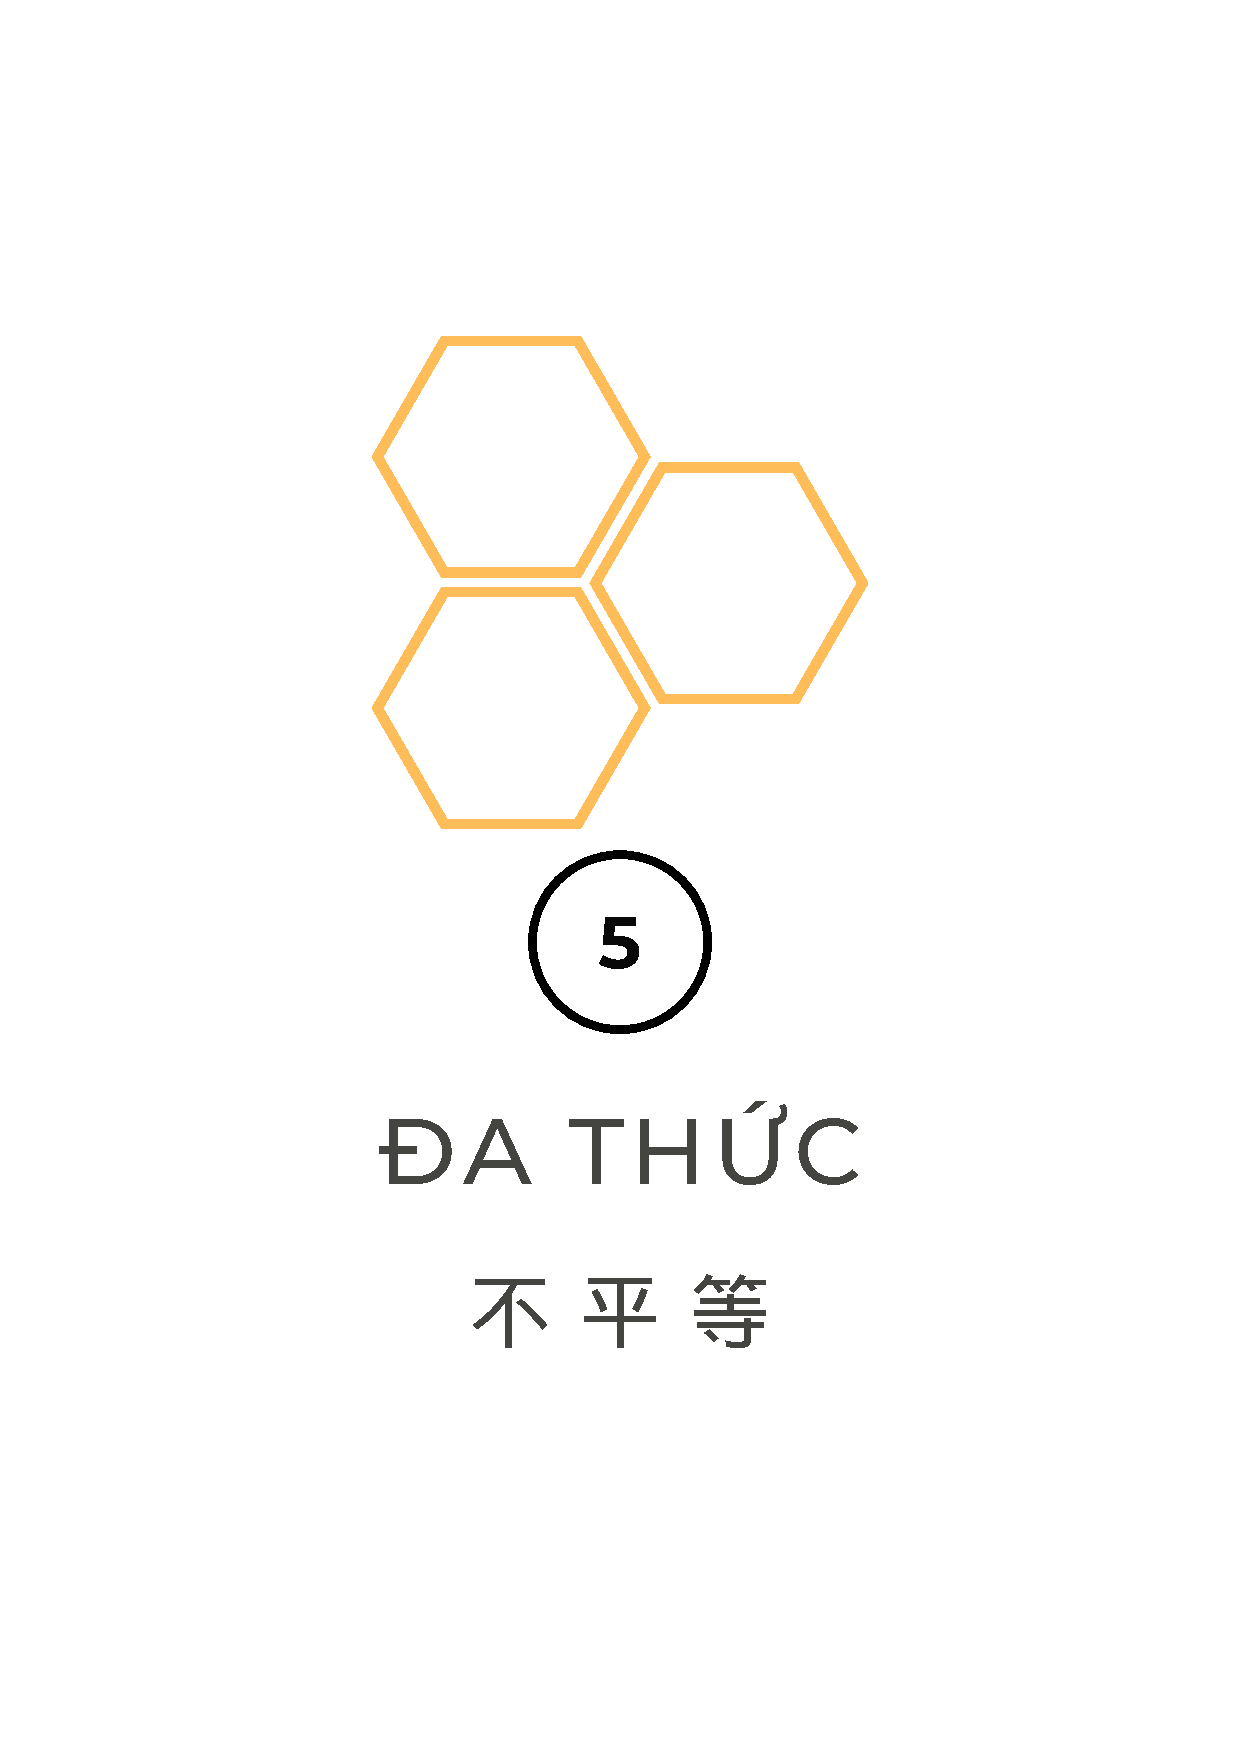
\includepdf[pages=1]{5.pdf}
        \section{\huge Đa thức}
        \subsection{\LARGE \textcolor{dk}{Đề bài}}
        \item \begin{btvn}\vocab{(Bulgaria TST 2015).}
            Tìm tất cả các đa thức hệ số thực $f(x) = \dsum_{i = 1}^{2n}$ có $2n$ nghiệm thực sao cho $|a_i| \leq 2$ với mọi $i = 1,2,\dots,n$
        \end{btvn}
        \item \begin{btvn}\vocab{(Romania TST 1990).}
            Cho $a \in \bb{Z}\backslash \{0\}$. Chứng minh rằng đa thức
            \[
                P(x) = x^n + ax^{n - 1} + \dots + ax - 1
            \]
            bất khả quy trên $Z[x]$.
        \end{btvn}
        \item \begin{btvn}\vocab{(Romania TST 1997).} Cho số nguyên $n \geq 2$ và đa thức
        \[
            P(x) = x^n + a_{n - 1}x^{n - 1} +\dots + a_1x+1
        \]
        là đa thức hệ số nguyên dương sao cho $a_k = a_{n - k}$ với mọi $k \in [n - 1]$. Chứng minh rằng tồn tại vô hạn cặp cặp số nguyên $(x,y)$ sao cho $x \mid P(y)$ và $y \mid P(x)$.
        \end{btvn}
        \item \begin{btvn}\vocab{(ITAMO 1994).}
            Cho đa thức $P(x) = a_0 + a_1x + \dots + a_{2n}x^{2n}$ là khai triển của biểu thức $(1 + x + x^2)^n$. Tính
            \begin{enumerate}[label=(\alph*)]
                \item $a_0 + a_2 + \dots + a_{2n}$
                \item $a_1 + a_3 + \dots + a_{2n - 1}$
                \item $a_0a_1 - a_1a_2 + a_2a_3 -\dots- a_{2n - 1}a_{2n}$
            \end{enumerate}
        \end{btvn}
        \item \begin{btvn}
            Cho $P(x) = a_nx^n + \dots + a_0$ là đa thức không âm với hệ số phức. Chúng ta nói rằng $P(x)$ là \textit{tương hỗ} nếu như $a_k = a_{n - k}$ với mọi $k \in \{0,1,\dots,n\}$ hoặc $a_k = -a_{n - k}$ với mọi $k \in \{0,1,\dots,n\}$. Với mỗi đa thức ta ký hiệu $[P(x)]$ như sau: 
            \begin{enumerate}
                \item $[P(x)] = 1$ nếu như $a_k = a_{n - k}$ với mọi $k \in \{0,1,\dots,n\}$
                \item $[P(x)] = -1$ nếu như $a_k = -a_{n - k}$ với mọi $k \in \{0,1,\dots,n\}$
            \end{enumerate}
            \begin{enumerate}[label=(\alph*)]
                \item Chứng minh rằng nếu như $P(x)$ và $Q(x)$ là \textit{tương hỗ} thì $P(Q(x))$ cũng tương hỗ và $[P(Q(x))] = [P(x)][Q(x)]$
                \item Chứng minh rằng nếu như $P(x)$ và $P(Q(x))$ là \textit{tương hỗ} thì $Q(x)$ là \textit{tương hỗ} và $[Q(x)] = \frac{[P(Q(x))]}{[P(x)]}$
            \end{enumerate}
        \end{btvn} 
        \item \begin{btvn} Cho đa thức monic $f(x) = \dsum_{i = 0}^n a_ix^i$ có các nghiệm thực $x_1,\dots,x_n$ thuộc đoạn $[-1,1]$ và hệ số thỏa mãn $a_{n - i} = a_i$, $i = 0,1,\dots,n$. Chứng minh rằng $f(x) = (x + 1)^p(x - 1)^{2q}$ với $p,q \in \bb{N}$ và $p + 2q = n$.
        \end{btvn}
        \item \begin{btvn}\vocab{(Romania MO).} Cho đa thức $P(x) = a_{2n}x^{2n} + a_{2n - 1}x^{2n - 1} +\dots + a_0$ sao cho $a_k = a_{2n - k}$ với $k = 0,1,\dots,n$
        \begin{enumerate}[label=(\alph*)]
            \item Chứng minh rằng tồn tại một đa thức $Q$ sao cho 
            \[  
                P(x) = x^nQ\left(x + \frac{1}{x}\right)
            \]
            \item Nếu $a_0 = a_{2n} = 1$ và $|a_{n}| < 2$. Chứng minh rằng $P(x)$ có ít nhất một nghiệm phức.
        \end{enumerate}
        \end{btvn}
        \item \begin{btvn}
            Cho đa thức $P(x) = a_dx^d + \dots + a_1 x + a_0$ và định nghĩa
            \[
                C(P(x)) = a_d^2 + a_{d - 1}^2 + ... + a_1^2 + a_0^2
            \]
            Cho $P(x) = 3x^2 + 7x + 2$. Tìm đa thức $Q(x)$ hệ số thực sao cho $Q(x) = 1$ và $C((P(x))^n) = C((Q(x))^n)$ với mọi số nguyên dương $n$.
        \end{btvn}
        \item \begin{btvn}\vocab{(VMO 1998).}
            Tìm tất cả các số nguyên dương $n$ sao cho tồn tại một đa thức $P(x)$ với hệ số thực thỏa mãn $P(x^{1998} - x^{-1998}) = x^n - x^{-n}$
        \end{btvn}
        \item \begin{btvn}
            Cho $n \equiv 0,1 \pmod{3}$. Chứng minh rằng đa thức $P(x) = x^n + x + 1$ bất khả quy trên $Z[x]$.
        \end{btvn}
        \item \begin{btvn}\vocab{(USA TST 2014).} Cho $n$ là số nguyên dương chẵn. Đặt $c_1,c_2,\dots,c_n$ là các số thực sao cho 
        \[
            \sum_{i = 1}^n |c_i - 1| < 1
        \]
        Chứng minh rằng đa thức 
        \[
            P(x) = 2x^n - c_{n - 1}x^{n - 1} + c_{n - 2}x^{n -2} -\dots-c_1x + 2
        \]
        không có nghiệm thực.
        \end{btvn}
        \item \begin{btvn}
            Cho $a_1,a_2,\dots,a_n$ là các số phức có module $r > 0$. Gọi $T_s$ là tổng của tích bất kì $s$ số từ $a_1,\dots,a_n$. Giả sử $T_{n - s} \neq 0$. Chứng minh rằng $\left|\frac{T_s}{T_{n - s}}\right| = r^{2s - n}$.
        \end{btvn}
        \item \begin{btvn}
            Cho đa thức $P(x) = b_dx^d + \dots + b_0$, chúng ta định nghĩa tổng $BB$ của $P(x)$ là $b_0b_1 + b_1b_2 +\dots+b_{d - 1}b_d$. Xác định rằng tồn tại hay không số thực $r$ và $s$ sao cho với mỗi số nguyên dương $k$, tổng $BB$ của $(x^2 + rs + s)^k$ bằng tổng $BB$ của $(2x^2 + 7x + 3)^k$.
        \end{btvn}
        \item \begin{btvn}
            Cho đa thức $P(x) = x^d + a_{d - 1}x^{ d- 1} + \dots + a_1x + a_0$ là đa thức có bậc $d \geq 3$ với hệ số nguyên sao cho $a_k + a_{d -k}$ là số chẵn với $k \in [d- 1]$ và $a_0$ cũng là số chẵn. Nếu như $P(x) = Q(x)R(x)$ trong đó $R(x)$ và $Q(x)$ là đa thức khác hằng hệ số nguyên và $\deg Q(x) \leq \deg R(x)$ với tất cả các hệ số của $R(x)$ đều lẻ. Chứng minh rằng $P(x)$ có ít nhất một nghiệm nguyên.
        \end{btvn}
        \item \begin{btvn}
            Cho $a \neq 0,b,c$ là các số thực. Chứng minh rằng tồn tại một đa thức hệ số thực $P(x)$ sao cho $x^2 + 1 \mid aP(x)^2 + bP(x) + c$.
        \end{btvn}
        \item \begin{btvn}
            Với $k,m,n$ là số nguyên không âm. Chứng minh rằng
            \[
                x^2 + x + 1 \mid x^{3k + 2} + x^{3m + 1} + x^{3n}
            \]
        \end{btvn}
        \item \begin{btvn}\vocab{(Poland MO 1986).}
            Chứng minh rằng với mỗi số nguyên dương $k$ ta luôn có
            \[
                x^5 + 1 \mid (x^4 - 1)(x^3 - x^2 + x - 1)^k + (x + 1)x^{4k - 1}
            \]
        \end{btvn}
        \item \begin{btvn}\vocab{(Poland MO 1988).}
            Cho đa thức $f(x)$ và $n$ là số nguyên dương. Chứng minh rằng nếu $f(x^n)$ chia hết cho $x - 1$ thế thì cũng chia hết cho
            \[
                x_{n - 1} + x_{n - 2} +\dots + x + 1
            \]
        \end{btvn}
        \item \begin{btvn}\vocab{(Poland MO 1996).}
            Tìm tất cả các cặp $(n,r) \in \bb{N} \times \bb{R}$ sao cho đa thức $(x + 1)^n - r$ chia hết cho $2x^2 + 2x + 1$.
        \end{btvn}
        \item \begin{btvn}
            Cho số thực $|a| \leq 1$. Chứng minh rằng tất cả các nghiệm của đa thức $x^{n + 1} -ax^n -ax + 1 = 0$ đều nằm trên đường tròn đơn vị.
        \end{btvn}
        \item \begin{btvn}\vocab{(USAMO 2014).}
            Cho các số thực $a,b,c,d$ thỏa mãn $b - d \geq 5$ và các nghiệm $x_1,x_2,x_3$ và $x_4$ của đa thức $P(x) = x^4 +ax^3 + bx^2 + cx + d$ là số thực. Tìm giá trị nhỏ nhất của
            \[
                (x_1^2 + 1)(x_2^2 + 1)(x_3^2 + 1)(x_4^2 + 1)
            \]
        \end{btvn}
        \item \begin{btvn}\vocab{(Mongolian MO 2018).}
            Tìm tất cả các đa thức $P(x)$ sao cho với mọi số thực $x,y,z$ thỏa mãn $x + y + z = 0$, ba điểm $(x,P(x)), (y,P(y)),(z,P(z))$ thẳng hàng trên mặt phẳng tọa độ.
        \end{btvn}

        \item \begin{btvn}\vocab{(Canada MO 2018).}
            Tìm tất cả các đa thức $P(x)$ hệ số thực thỏa mãn tính chất: tồn tại một đa thực hệ số thực $Q(x)$ hệ số thực sao cho
            \[
                P(1) + P(2) + \dots + P(n) = P(n)Q(n)
            \]
            với mọi số nguyên dương $n$
        \end{btvn}

        \item \begin{btvn}
            Cho đa thức $P(x) = x^2 + a$ ($a \neq 0$) và $Q(x) = x^3 + bx + c$. Nếu như $Q(P(x)) = P(Q(x))$ với mọi số thực $x$, tìm giá trị của $Q(10)$.
        \end{btvn}

        \item \begin{btvn}\vocab{(Czech-Slovak 2001).}
            Tìm tất cả các đa thức $P(x)$ thỏa mãn
            \[P(2x) = 8P(x) + (x - 2)^2, \forall x \in \bb{R}\]
        \end{btvn}

        \item \begin{btvn}
            Cho đa thức $P(x)$ thỏa mãn
            \[
                3P(x^2) + 2122x^2 = 2(x^2 + 2)P(x) + x^4 + 4024x^3 + 8048x + 1959
            \]
            Tính $P(2013)$.
        \end{btvn}

        \item \begin{btvn}
            Tìm tất cả đa thức $P(x)$ và $Q(x)$ hệ số thực thỏa mãn
            $$
            \begin{gathered}
            P(Q(x)+1)=1+Q(P(x)) \\
            Q(P(x)+1)=1+P(Q(x)) \\
            P(0)=Q(0)=0
            \end{gathered}
            $$
        \end{btvn}

        \item \begin{btvn}
            Tìm tất cả đa thức $P(x)$ hệ số thực thỏa mãn
            $$
            P(x) P(y)=P\left(\frac{x+y}{2}\right)^2-P\left(\frac{x-y}{2}\right)^2
            $$
        \end{btvn}

        \item \begin{btvn}
            Tìm tất cả đa thức $P(x)$ hệ số phức thỏa mãn $P(0)=0$ và với mọi số nguyên dương $n>2$ và với mọi số thực $a_1, a_2, \ldots, a_n$ với $a_1+a_2 \ldots+a_n \neq 0$ thì có
                $$
                P\left(\frac{a_1}{a_1+a_2+\ldots+a_n}\right)+\ldots+P\left(\frac{a_n}{a_1+a_2+\ldots+a_n}\right)=0
                $$
        \end{btvn}

        \item \begin{btvn}
            Cho $P(x)$ là đa thức không âm thỏa mãn
            $$
            P(x)(x-1)^{20}=\left(x^2+a x+1\right)^{30}+\left(x^2+b x+c\right)^{10}
            $$
            với các số thực $a, b, c$. Tính $P(1)+a^2+b^2+c^2$.
        \end{btvn}

        \item \begin{btvn}
            Tìm tất cả đa thức monic $P(x)$ hệ số thực sao cho với mọi số thực $x$ ta có
            $$
            P(x+P(x))=x^2+P(P(x)) .
            $$
        \end{btvn}

        \item \begin{btvn}
            Cho các ý sau:

            (a) Tìm tất cả đa thức hệ số thực $P(x)$ thỏa mãn $(x-4) P(x+1)-x P(x)+20=0, \forall x \in \mathbb{R}$.

            (b) Từ các nghiệm đa thức của câu (a), tìm đa thức thỏa mãn $P(0) = 29$.
        \end{btvn}

        \item \begin{btvn}
            Cho đa thức $P(x)$ hệ số nguyên sao cho $P(a) = 1$, $P(b) = 2$ và $P(17) = 3$ với một vài số nguyên $a < b < 17$
            \begin{enumerate}[label=(\alph*)]
                \item Chứng minh rằng phương trình $P(x) = 5$ có nhiều nhất một nghiệm nguyên.
                \item Tìm tất cả đa thức $P(x)$ sao cho với phương trình $P(x) = 5$ có chính xác một nghiệm nguyên.
            \end{enumerate}
        \end{btvn}

        \item \begin{btvn}
            Anna đang chơi một trò chơi toán học trên máy tính. Máy tính đang ẩn đa thức $P(x)$. Anna chưa biết bậc và các hệ số của $P(x)$ , nhưng cô ấy biết rằng các hệ số này hoàn toàn là số thực dương. Ở mỗi lần di chuyển, Anna nhập một số thực $a$ và máy tính xuất ra $P(a)$. Điều này được lặp lại cho đến khi Anna có thể xác định được $P(x)$. Đối với chiến lược $S$ được Anna sử dụng, biểu thị bằng $S(P)$ số bước đi mà cô ấy cần để xác định $P(x)$. Gọi một chiến lược $S$ tối ưu nếu $S(P) \leq S^{\prime}(P)$ cho tất cả các chiến lược có thể $S^{\prime}$ và tất cả các đa thức $P$ với hệ số dương. Có tồn tại hay không một chiến lược tối ưu?
        \end{btvn}

        \item \begin{btvn}\vocab{(Czech-Slovak 2001).}
            Tìm tất cả các đa thức $P$ và $Q$ sao cho với mọi số thực $x$ thì 
                $$
                Q\left(x^2\right)=(x+1)^4-x(P(x))^2
                $$
        \end{btvn}

        \item \begin{btvn}
        Tìm tất cả các đa thức $P(x)$ hệ số thực thỏa mãn
            $$
            P\left(x^2\right) P\left(x^3\right)=(P(x))^5 \quad \forall x \in \mathbb{R} .
            $$
        \end{btvn}

        \item \begin{btvn}
            Tìm tất cả các cặp đa thức $P(x)$ và $Q(x)$ hệ số thực thỏa mãn $x^3 Q(x)=P(Q(x))$ với mọi số thực $x$.
        \end{btvn}

        \item \begin{btvn}
            Tìm tất cả đa thức hệ số thực $P(x)$ thỏa mãn
            $$
            P(x)^2-P(x-1) P(x+1)=2 P(x)
            $$
        \end{btvn}

        \item \begin{btvn}
            Tìm tất cả đa thức hệ số thực $P(x)$ thỏa mãn
            $$
            P(x-1) P(x+1)>P(x)^2-1
            $$
        \end{btvn}

        \item \begin{btvn}\vocab{(Canada MO 2013).}
            Tìm tất cả đa thức hệ số thực $P(x)$ sao cho
            $$
            (x+1) P(x-1)-(x-1) P(x)
            $$
            là một hằng số
        \end{btvn}

        \item \begin{btvn}\vocab{(Czech-Slovak 2002).}
            Tìm tất cả đa thức hệ số thực $P(x)$ thỏa mãn
            $$
            (x+1) P(x-1)+(x-1) P(x+1)=2 x P(x) 
            $$
        \end{btvn}

        \item \begin{btvn}\vocab{(Belarus MO 2013).}
        Tìm tất cả đa thức hệ số thực $P(x)$ thỏa mãn
            $$
            (x-1) P(x+1)-(x+1) P(x-1)=4 P(x)
            $$
        \end{btvn}

        \item \begin{btvn}\vocab{(VMO 1984).} Cho $a,b$ là các số thực với $a \neq 0$. Tìm tất cả các đa thức $P(x)$ thỏa mãn
            $$
            x P(x-a)=(x-b) P(x) \quad \forall x
            $$
        \end{btvn}

        \item \begin{btvn}\vocab{(VMO 2002).}
            Tìm tất cả các đa thức $P(x)$ hệ số thực thỏa mãn
            \[
                (x^3 + 3x^2 + 3x + 2)P(x - 1) = (x^3 - 3x^2 + 3x -2)P(x)
            \]
        \end{btvn}

        \item \begin{btvn}
            Cho đa thức $R(t)$ có bậc là 2017. Chứng minh rằng tồn tại vô hạn đa thức $P(x)$ thỏa mãn
            \[
                P((R^{2014}(t) + R(t) + 1)^2 - 2) = P(R^{2017}(t) + R(t) + 1)^2 - 2
            \]
            Tìm mối quan hệ giữa các đa thức $P(x)$.
        \end{btvn}

        \item \begin{btvn}\vocab{(Taiwan TST 2014)}
            Tìm tất cả các đa thức $P(x)$ hệ số thực thỏa mãn
            \[
                P(x)P(x + 1) = P(x^2 - x + 3)
            \]
        \end{btvn}

        \item \begin{btvn}
            Cho đa thức $P(x) \in \bb{Z}[x]$ là đa thức bất khả quy có các nghiệm có giá trị tuyệt đối lớn hơn $\frac{3}{2}$. Chứng minh rằng nếu $P(\alpha) = 0$ thì $P(1 + \alpha^3) \neq 0$.
        \end{btvn}
        \item \begin{btvn}\vocab{(Gazeta 11/2011).}
            Cho đa thức $f \in \bb{Z}[x]$ là đa thức monic và dãy số $(a_n)$ là một cấp số cộng của số tự nhiên. Chứng minh rằng nếu tồn tại $k \in \bb{Z}$ với $a_1 = f(k)$ thì tập hợp
            \[
                \{a_n \mid n \geq 1\} \cap \{f(n) \mid n \in \bb{Z}\}
            \]
            là vô hạn.
        \end{btvn}

        \item \begin{btvn}
            Cho đa thức hệ số nguyên $P(x)$ có bậc là $d$ sao cho với một vài số nguyên tố $q > d$ ta có $P(k) \equiv 0 \pmod(q)$ với mọi $k$. Chứng minh rằng mọi hệ số của $P(x)$ đều chia hết cho $q$.
        \end{btvn}

        \item \begin{btvn}
            Chứng minh rằng mọi đa thức 
            \[
                P(x) = a_0 + a_1x +\dots + a_{n - 1}x^{n - 1}
            \]
            có thể được viết dưới dạng
            \[
                P(z) = \frac{1}{n}\dsum_{k = 1}^n w_kP(w_k) \frac{z^n - 1}{z - w_k}
            \]
            Trong đó $w_1,w_2,\dots, w_n$ là các căn nguyên thủy bậc $n$.
        \end{btvn}

        \item \begin{btvn}
            Cho đa thức hệ số thực $Q(x)$ có bậc là $d$. Xét dãy số thực $b_1 < \dots < b_{d + 1}$. Chứng minh rằng đa thức
            \[
                f(x) = \sum_{i = 1}^{d + 1}a_iQ(x + b_i)
            \]
            là đa thức hằng với $a_i = \dprod_{i \neq j}\frac{1}{b_i - b_j}$
        \end{btvn}

        \item \begin{btvn}\vocab{(VMO 2011).}
            Cho $n\in\mathbb N$ và đa thức $P(x,y)=x^n+xy+y^n.$
            Chứng minh rằng chúng ta không thể thu được hai đa thức khác hằng $G(x,y)$ và $H(x,y)$ với các hệ số thực sao cho
            $P(x,y)=G(x,y)\cdot H(x,y).$
        \end{btvn}

        \item \begin{btvn}\vocab{(VMO 2012).}
            Cho $\langle a_n\rangle $ và $ \langle b_n\rangle$ là hai dãy cấp số cộng, và cho $m$ là một số nguyên lớn hơn $ 2$. Xét đa thức $P_k(x)=x^2+a_kx+b_k,\ k=1,2,\cdots, m.$ Chứng minh rằng nếu các biểu thức bậc hai $P_1(x), P_m(x)$  không có bất kỳ nghiệm thực nào, thì tất cả các đa thức còn lại cũng không có nghiệm thực.
        \end{btvn}

        \item \begin{btvn}\vocab{(VMO 2015).}
            Cho ${\left\{ {f(x)} \right\}}$ là một dãy đa thức, trong đó ${f_0}(x) = 2$, ${f_1}(x) = 3x$, và

            $${f_n}(x) = 3x{f_{n - 1}}(x) + (1 - x - 2{x^2}){f_{n - 2}}(x),n \ge 2$$

            Xác định giá trị của $n$ sao ${f_n}(x)$ cho chia hết cho $x^3-x^2+x$ .
        \end{btvn}

        \item \begin{btvn}\vocab{(VMO 2017).}
            Có tồn tại hay không đa thức hệ số nguyên $P(x)$ thỏa mãn\[ \begin{cases} P(1+\sqrt[3]{2})=1+\sqrt[3]{2}\\ P(1+\sqrt{5})=2+3\sqrt{5}\end{cases} \]
        \end{btvn}
        \item \begin{btvn}\vocab{(VMO 2019).}
            Với mỗi đa thức hệ số thực$f(x)={{a}_{0}}+{{a}_{1}}x+\cdots +{{a}_{n}}{{x}^{n}}$, ta định nghĩa 
            $$\Gamma (f(x))=a_{0}^{2}+a_{1}^{2}+\cdots +a_{m}^{2}.$$
            Cho đa thức $P(x)=(x+1)(x+2)\ldots (x+2020).$ Chứng minh rằng tồn tại ít nhất $2019$ cặp ${{Q}_{k}}(x)$ đa thức riêng biệt với $1\le k\le {{2}^{2019}}$ và mỗi đa thức thỏa mãn hai điều kiện sau:
            \begin{enumerate}
                \item $\deg {{Q}_{k}}(x)=2020.$
                \item $\Gamma \left( {{Q}_{k}}{{(x)}^{n}} \right)=\Gamma \left( P{{(x)}^{n}} \right)$ với mọi số nguyên dương $n$.
            \end{enumerate}

        \end{btvn}
        
        \item \begin{btvn}\vocab{(VMO 2021).}
            Cho đa thức $P(x)=a_{21}x^{21}+a_{20}x^{20}+\cdots +a_1x+a_0$ trong đó $1011\leq a_i\leq 2021$ với mọi $i=0,1,2,...,21,$ Cho có $P(x)$ có một nghiệm nguyên và tồn tại một số thực dương $c$ sao cho $|a_{k+2}-a_k|\leq c$ với mọi $k=0,1,...,19.$
            \begin{enumerate}[label=(\alph*)]
                \item Chứng minh rằng $P(x)$ có một nghiệm nguyên duy nhất.
                \item Chứng minh rằng$$\sum_{k=0}^{10}(a_{2k+1}-a_{2k})^2\leq 440c^2.$$
            \end{enumerate}
        \end{btvn}
        \item \begin{btvn}\vocab{(VMO 2024).}
            Tìm tất cả các đa thức có hệ số thực $P(x), Q(x)$ sao cho với mọi số thực $a$, $P(a)$ là một nghiệm của phương trình $$x^{2023}+Q(a)x^2+(a^{2024}+a)x+a^3+2025a=0$$
        \end{btvn}
        \item \begin{btvn}\vocab{(VMO 2024).}
            Với mỗi đa thức $P(x)$, ta định nghĩa 
            $$P_1(x)=P(x), \forall x \in \mathbb{R},$$$$P_2(x)=P(P_1(x)),  \forall x \in \mathbb{R},$$$$...$$$$P_{2024}(x)=P(P_{2023}(x)), \forall x \in \mathbb{R}.$$
            Cho $a>2$ là một số thực. Tồn tại hay không một đa thức $P$ với các hệ số thực sao cho với mọi $t \in (-a, a)$, phương trình $P_{2024}(x)=t$ có $2^{2024}$ nghiệm thực riêng biệt?
        \end{btvn}
        \item \begin{btvn}\vocab{(VNTST 2014).}
            Tìm tất cả các đa thức $P(x),Q(x)$ hệ số nguyên thỏa mãn: Cho dãy $(x_n)$ được định nghĩa bởi:
            \[x_0=2014,x_{2n+1}=P(x_{2n}),x_{2n}=Q(x_{2n-1}) \quad n\geq 1\]
            thì với mọi số nguyên dương $m$ đều là ước số của một phần tử khác không trong $(x_n )$
        \end{btvn}
        \item \begin{btvn}\vocab{(VNTST 2015).}
            Cho $\alpha$ là nghiệm dương của phương trình $x^2+x=5$. Cho $n$ là một số nguyên dương, và $c_0,c_1,\ldots,c_n\in \mathbb{N}$ sao cho $ c_0+c_1\alpha+c_2\alpha^2+\cdots+c_n\alpha^n=2015. $
            \begin{enumerate}[label=(\alph*)]
                \item Chứng minh rằng $c_0+c_1+c_2+\cdots+c_n\equiv 2 \pmod{3}$.
                \item Tìm giá trị nhỏ nhất của tổng $c_0+c_1+c_2+\cdots+c_n$.
            \end{enumerate}
        \end{btvn}
        \item \begin{btvn}\vocab{(VNTST 2016).}
            
        Cho $16$ số thực phân biệt $\alpha_1,\alpha_2,...,\alpha_{16}$. Đối với mỗi đa thức $P$, ký hiệu
        \[ V(P)=P(\alpha_1)+P(\alpha_2)+...+P(\alpha_{16}). \]
        Chứng minh rằng tồn tại một đa thức $Q$ monic, $\deg Q=8$ thỏa mãn:
            \begin{enumerate}
                \item $V(QP)=0$ đối với tất cả các đa thức $P$ có $\deg P<8$.
                \item $Q$ có $8$ nghiệm thực (bao gồm cả nghiệm bội).
            \end{enumerate}
        \end{btvn}
        \item \begin{btvn}\vocab{(VNTST 2018).}
            Cho mỗi số nguyên dương $n\ge 3$, đặt $\phi_n$ là tập hợp của tất cả các số nguyên dương nhỏ hơn và nguyên tố cùng nhau với $n$. Xét đa thức:
            $$P_n(x)=\sum_{k\in\phi_n} {x^{k-1}}.$$
            \begin{enumerate}[label=(\alph*)]
                \item  Chứng minh rằng $P_n(x)=(x^{r_n}+1)Q_n(x)$ với một số nguyên dương $r_n$ và đa thức $Q_n(x)\in\mathbb{Z}[x]$ (không nhất thiết phải là đa thức không hằng số).
                \item Tìm tất cả các $n$ sao cho $P_n(x)$ bất khả quy được trên $\mathbb{Z}[x]$.
            \end{enumerate}
        \end{btvn}
        \item \begin{btvn}\vocab{(VNTST 2019).}
            Với mỗi số nguyên dương $n$, chứng minh rằng đa thức$$P_n(x)=\sum _{k=0}^n2^k\binom{2n}{2k}x^k(x-1)^{n-k}$$ có $n$ nghiệm thực.
        \end{btvn}
        \item \begin{btvn}\vocab{(VNTST 2023).} Cho ba hàm số
            $$P(x) = (x^2-1)^{2023}, Q(x) = (2x+1)^{14}, R(x) = \left(2x+1+\frac 2x \right)^{34}.$$
            Ban đầu, chúng ta chọn một tập hợp $S$ chứa hai trong ba hàm này, và thực hiện một số phép toán trên nó. Các phép toán được phép bao gồm:
            \begin{enumerate}
                \item Chúng ta có thể lấy hai hàm $p, q \in S$ và thêm một trong các hàm $p+q, p-q$, hoặc $pq$ vào $S$.
                \item Chúng ta có thể lấy một hàm $p \in S$ và thêm $p^k$ vào $S$ với $k$ là một số nguyên dương tùy ý mà chúng ta chọn.
                \item Chúng ta có thể lấy một hàm $p \in S$ và chọn một số thực $t$, và thêm vào $S$ một trong các hàm $p+t, p-t, pt$.
            \end{enumerate}
            
            Chứng minh rằng dù chúng ta chọn $S$ như thế nào ở ban đầu, không có cách nào chúng ta có thể thực hiện một số phép toán hữu hạn trên $S$ mà cuối cùng sẽ cho ra hàm thứ ba không thuộc $S$.
        \end{btvn}
        \item \begin{btvn}\vocab{(VNTST 2024).}
            Cho $P(x) \in \mathbb{R}[x]$ là một đa thức monic, khác hằng. Tìm tất cả các hàm liên tục $f: \bb{R} \to \bb{R}$ thỏa mãn
            $$f(f(P(x))+y+2023f(y))=P(x)+2024f(y)$$
            với mọi số thực $x,y$.
        \end{btvn}
        \item \begin{btvn}\vocab{(VNTST 2024).}
            Cho $\alpha \in (1, +\infty)$ là một số thực, và cho $P(x) \in \mathbb{R}[x]$ là một đa thức monic với bậc $24$, sao cho
            \begin{enumerate}
                \item $P(0) = 1$.
                \item $P(x)$ có chính xác $24$ nghiệm thực dương mà tất cả đều nhỏ hơn hoặc bằng $\alpha$.
            \end{enumerate}
            Chứng minh rằng $|P(1)| \le \left( \frac{19}{5}\right)^5 (\alpha-1)^{24}$.
        \end{btvn}
        \item \begin{btvn}\vocab{(VNTST 2024).}
           Cho đa thức $P(x) \in \mathbb{Z}[x]$. Tìm tất cả các đa thức $Q(x) \in \mathbb{Z}[x]$, sao cho với mọi số nguyên dương $n$, tồn tại một đa thức $R_n(x) \in \mathbb{Z}[x]$ thỏa mãn
            $$Q(x)^{2n} - 1 = R_n(x)\left(P(x)^{2n} - 1\right).$$
        \end{btvn}
        \item \begin{btvn}\vocab{(IMOSL 2013 A6).} Cho $m \neq 0$ là số nguyên. Tìm tất cả các đa thức hệ số thực thỏa mãn:
        \[
            (x^3 - mx^2 + 1)P(x + 1) + (m^3 + mx^2 + 1)P(x - 1) = 2(x^3 - mx + 1)P(x)
        \]
        với mọi số thực $x$.
        \end{btvn}
        \item \begin{btvn}\vocab{(IMOSL 2014 A5).} Xét các đa thức $P(x)$ với hệ số thực thỏa mãn tính chất sau: với hai số thực bất kỳ $x$ và $y$ thì ta có \[|y^2-P(x)|\le 2|x|\quad\text{ khi và chỉ khi }\quad |x^2-P(y)|\le 2|y|.\]Tìm tất cả các giá trị của $P(0)$.
        \end{btvn}
        \item \begin{btvn}\vocab{(IMOSL 2015 A6).} Cho $n$ là một số nguyên cố định với $n \ge 2$. Chúng ta nói rằng hai đa thức $P$ và $Q$ có hệ số thực là \textit{tương tự} với nhau nếu với mỗi $i \in \{1, 2, \ldots, n\}$ các dãy
            \begin{eqnarray*}
                P(2015i), P(2015i - 1), \ldots, P(2015i - 2014) & \text{và}\\
                Q(2015i), Q(2015i - 1), \ldots, Q(2015i - 2014)
            \end{eqnarray*}
        là hoán vị của nhau.
        \begin{enumerate}[label=(\alph*)]
            \item Chứng minh rằng tồn tại các đa thức \textit{tương đương} nhau có bậc là $n + 1$.
            \item Chứng minh không tồn tại các đa thức \textit{tương đương} nhau có bậc là $n$.
        \end{enumerate}
        \end{btvn}
        \item \begin{btvn}\vocab{(IMOSL 2022 A7).}
            Với mọi số nguyên dương \( n \), ta ký hiệu \( s(n) \) là tổng của các chữ số của \( n \). Xét đa thức \( P(x) = x^n + a_{n-1}x^{n-1} + \cdots + a_1x + a_0 \), trong đó \( n \geqslant 2 \) và \( a_i \) là một số nguyên dương cho mọi \( 0 \leqslant i \leqslant n-1 \). Có thể có trường hợp nào mà, với mọi số nguyên dương \( k \), \( s(k) \) và \( s(P(k)) \) có cùng tính chẵn lẻ không?

        \end{btvn}
        \subsection{\LARGE \textcolor{dk}{Lời giải}}
\end{itemize}
\end{document}